% Reformatted thesis, February 2015
% The Subregular Germ of Orbital Integrals
% Thomas C. Hales

%% XX issues.
%% \definition ... \enddefinition marks many equations, comments, etc.
%% unnumbered remarks throw off count.
%% fix bibliography.

\documentclass{memo-l}

%    For use when working on individual chapters
%\includeonly{}

%    Include referenced packages here.
\usepackage{amsrefs}
\usepackage{enumitem}
\usepackage{amsthm}
\usepackage{longtable}
\usepackage{amscd}

%tikz graphics
%\usepackage{xcolor} % to remove color.
\usepackage{tikz} 
\usetikzlibrary{chains,shapes,arrows,shadings,trees,matrix,%
  positioning,intersections,decorations,%
  decorations.markings,decorations.pathmorphing,backgrounds,%
  fit,calc,fadings,decorations.pathreplacing}
%\usepackage{tikz-cd} % commutative diagrams.

% fonts

%\usepackage{mathrsfs}
\usepackage{}

\newtheorem{theorem}{Theorem}[section]
\newtheorem{lemma}[theorem]{Lemma}
\newtheorem{corollary}[theorem]{Corollary}
\newtheorem{proposition}[theorem]{Proposition}

\theoremstyle{definition}
\newtheorem{definition}[theorem]{Definition}
\newtheorem{example}[theorem]{Example}
\newtheorem{xca}[theorem]{Exercise}

\theoremstyle{remark}
\newtheorem{remark}[theorem]{Remark}
\newtheorem*{remark*}{Remark} % unnumbered remark
\newtheorem*{eqn*}{Equation} % unnumbered eqn
\newtheorem{eqn}[theorem]{Equation}
\newtheorem{assumption}[theorem]{Assumption}
\newtheorem{fact}{Fact}
\newtheorem{rem}{Remark}
\newtheorem{case}{Case}
%\newtheorem{case*}{Case}

\def\tikzfig#1#2#3{%
\begin{figure}[htb]%
  \centering
\begin{tikzpicture}#3
\end{tikzpicture}
  \caption{#2}
  \label{fig:#1}%
\end{figure}%
}



\numberwithin{section}{chapter}
\numberwithin{equation}{chapter}

\renewcommand\thechapter       {\Roman{chapter}}


%    For a single index; for multiple indexes, see the manual
%    "Instructions for preparation of papers and monographs:
%    AMS-LaTeX" (instr-l.pdf in the AMS-LaTeX distribution).
\makeindex

\begin{document}

\frontmatter

\title{The Subregular Germ of Orbital Integrals}
\author{Thomas C. Hales}
\address{University of Pittsburgh 15260}
%\curraddr{}
\email{}
\thanks{Memoirs of the AMS, Number 476. Copyright 1992, AMS}
%    \date is required; it is the date received by the editor.
\date{February 20, 1989}

\subjclass[2010]{Primary }
%    Recognition of the 2010 edition of the Mathematics Subject
%    Classification requires a version of amsbook.cls from July 2009
%    or later.  If "2010" is not recognized, please upgrade.

\keywords{}

%\dedicatory{Dedication text (use \\[2pt] for line break if necessary)}

\maketitle

\tableofcontents

\begin{abstract}
  An integral formula for the subregular germ of a $\kappa$-orbital
  integral is developed.  The formula holds for any reductive group
  over a $p$-adic field of characteristic zero.  This expression of
  the subregular germ is obtained by applying Igusa's theory of
  asymptotic expansions.  The integral formula is applied to the
  question of the transfer of a $\kappa$-orbital integral to an
  endoscopic group.  It is shown that the quadratic characters arising
  in the subregular germs are compatible with the transfer.  Details
  of the transfer are given for the subregular germ of unitary groups.
\end{abstract}

%    Include unnumbered chapters (preface, acknowledgments, etc.) here.
%\include{}

%    Include main chapters here.
%\include{}



%-----------------------------------------------------------------------
% End of memo-l-template.tex
%-----------------------------------------------------------------------

\input diagram.tex

%\hoffset=.5in \voffset=0.5in

%Blackboard bold symbols

\newcommand\AAA{{\Bbb A}}                   \newcommand\BB{{\Bbb B\,}}
\newcommand\CC{{\Bbb C}}                    \newcommand\GG{{\Bbb G}}
\newcommand\PP{{\Bbb P}}                    \newcommand\RR{{\Bbb R}}
\newcommand\TT{{\Bbb T}}                    \newcommand\ZZ{{\Bbb Z}}
\newcommand\bWW{{\Bbb W}}                       \newcommand\bW{\bold{W}}

%\newcommand\bWW{{\Bbb W}}
 \newcommand\bP{{\bold P}} % was \PP redefined in dthis.tex
%\newcommand\bW{\bold{W}}

% Greek symbols:

%\newcommand\a{\alpha}  %already in use
%\newcommand\b{\beta}
%\newcommand\d{\delta}
\newcommand\g{\gamma}
\newcommand\e{\epsilon}
\newcommand\z{\zeta}



%A few abbreviations:

\newcommand\Gal{{\operatorname{Gal}(\bar F/F)}}
\newcommand\GalK{{\operatorname{Gal}(K/F)}}
\newcommand\Fb{{\bar F}}
\newcommand\back{\backslash}



%Codes for references:

%\newcommand\A{1}                % not found
%\newcommand\Ba{2}
%\newcommand\Ca{3}               % not found
%\newcommand\GR{4}
%\newcommand\HCa{5} %MR0579175
%\newcommand\HCb{6} %MR0340486 % not found
% \newcommand\Ha{7} % MR0463157
%\newcommand\Hi{8} % MR0102519
%\newcommand\Hib{9} % MR480502
%\newcommand\Hu{{10}} % MR0396773
%\newcommand\Ig{{11}} %MR546292
%\newcommand\Ko{{12}} %MR683003
%\newcommand\Kn{{13}} %MR0188219,MR0174559
%\newcommand\Lan{{14}} %MR697567
%\newcommand\LL{{15}} %MR701566
%\newcommand\LSa{{16}} %MR748510
%\newcommand\LSb{{17}} %MR909227
%\newcommand\M{{18}} %MR971985
%\newcommand\Se{{19}} %MR0150130 %not found
%\newcommand\Ser{{20}} %MR0180551
%\newcommand\Sl{{21}} %MR584445
%\newcommand\Spal{{22}} %MR672610
%\newcommand\St{{23}} %MR0352279

\def\fitem#1{{\par\noindent #1}}

%% temp defs to get it to tex
\newcommand\leaderfill{\ldots}
\newcommand\itemitem{}
%\newcommand\topmatter{}
\newcommand\head{}
\newcommand\sendhead{}
\newcommand\widestnumber{}
\newcommand\specialhead{}
\newcommand\page{}
\newcommand\sendspecialhead{}
\newcommand\subhead{}
\newcommand\sendsubhead{}
\newcommand\sendtoc{}
\newcommand\sendtitle{}
\newcommand\sendtopmatter{}
\newcommand\prelax{} % marks pmatrix
\newcommand\medpagebreak{}
\newcommand\dsize{}
\newcommand\etag{\quad}
%\newcommand\no{}
\newcommand\by{}
\newcommand\paper{}
\newcommand\book{}
\newcommand\inbook{}
\newcommand\publ{}
\newcommand\publaddr{}
\newcommand\yr{}
\newcommand\sendref{}
\newcommand\bookinfo{}
\newcommand\jour{}
\newcommand\vol{}
\newcommand\pages{}
\newcommand\sline{}




%% start ithis.tex Forward March 1991

\chapter*{Introduction}

An elementary fact in the theory of finite groups states that the vector
space spanned by irreducible characters of representations of a group coincides
with the vector space spanned by characteristic functions of conjugacy classes.
To give an explicit formula for an irreducible character is to express a character
as a linear combination of the basis vectors formed by characteristic functions.
For Lie groups or $p$-adic groups, irreducible characters must be interpreted
as distributions.  Similarly the characteristic functions must be replaced by
distributions, orbital integrals,  supported on the conjugacy classes if one
hopes to develop systematically a theory of characters on Lie and $p$-adic groups.
A successful character theory of these groups should give relations expressing
distribution characters as linear combinations of orbital integrals, and
orbital integrals as sums of characters.  This work is concerned
with the study of orbital integrals on $p$-adic groups, needed for eventual applications
to automorphic representation theory and the trace formula.

These orbital integrals have a notoriously complicated structure.  As
the conjugacy class is allowed to vary, the orbital integrals possess
an asymptotic expansion called the Shalika germ expansion.  In
contrast to what the terminology might suggest, the asymptotic
expansion has only finitely many terms and for $p$-adic groups
actually gives an exact formula for the orbital integral in a
sufficiently small neighborhood of the identity element.  Moreover, by
inductive arguments the behavior of an orbital integral may be
understood once its behavior near the identity element of the group is
understood.  Consequently most questions we might have about orbital
integrals can be answered from Shalika's expansion.  Unfortunately,
Shalika's {\it existence} proof of an asymptotic expansion has not
resulted in explicit formulas for the germs except in a few elementary
cases.

A basic problem of harmonic analysis on reductive $p$-adic groups is
then to develop expressions for the terms of the Shalika expansion of
orbital integrals.  This work uses a geometrical approach, introduced
by Langlands and Shelstad, to calculate the first two terms of the
Shalika expansion.  These terms are called the regular and subregular
terms of the expansion.  The first term of the expansion is, with
suitable normalizations of measures, an invariant integral over the
stable regular unipotent class.  The second term of the expansion, as
we will see, is a sum of integrals of the form
\[
 \theta(\lambda)|\lambda|\int_{\PP^1} {\frac {dv}{|v|}}
\int_{\PP^1}\eta(p(w))\frac {dw}{|w|^2} \mu_0
\]
where $p$ is an appropriate polynomial in $w$; and $\eta$, $\theta$
are multiplicative characters on the $p$-adic field $F$. Also $\mu_0$
is an invariant integral over a subregular unipotent conjugacy class
of the group.  These integrals over projective lines must be
understood as principal value integrals.

The explicit formulas for the first two terms of the Shalika expansion
allow us to check a number of conjectures concerning orbital integrals
-- many of which were known previously only for a few groups of small
rank.  This method used here to obtain explicit formulas for Shalika
germs remains the only known general method to obtain such formulas.
Other methods are now available for the general and special linear
groups.


Here are a few remarks on the geometrical construction of Shalika
germs.  If $\Gamma$ is a curve inside a Cartan subgroup $T$ of $G$
such that $\Gamma(0) = 1\in T$ and $\Gamma(s)$, $s\ne0$ is a regular
element of $T$, then the conjugacy class of $\Gamma(s)$, $s\ne0$ may
be identified with $\Gamma(s)\times T\back G$ and the Shalika germ
expansion gives the asymptotics of integrals on $\Gamma(s)\times
T\back G$ as $s$ tends to $1$.  The essential part of the construction
of Shalika germs is the construction of a $G$-equivariant completion
$Y\to^\pi\Gamma$ of $\Gamma\times T\back G\to^\pi \Gamma$.  The theory
of Igusa then states that the asymptotic expansion as $s$ tends to $1$
may be understood by studying the divisor $D=\pi^{-1}(\Gamma(1))$ in
the variety $Y$.  Roughly each term of the asymptotic expansion is an
integral over some of the irreducible components of $D$.

To see some of the technical difficulties involved in this procedure,
consider two completions $Y_1$, $Y_2$ of $\Gamma\times T\back G$ with
corresponding divisors $D_1$ and $D_2$.  The fact that the asymptotic
expansion is independent of the completion shows that the terms of the
expansion (integrals over components of $D_1$ and $D_2$) coincide.
This suggests that these integrals on $D_1$ and $D_2$ should be
invariant under a large class of birational maps.  This is indeed the
case.  In the special case that $Y_1$ is obtained from $Y_2$ by
blowing up $Y_1$ along a subvariety of $D_1$, it suggests that the
exceptional divisors introduced by blowing up usually make no
contribution to the asymptotic expansion.  In other words, if we begin
with a completion $Y_1$ which is far from being a minimal completion,
it will be necessary to sort through a large number of exceptional or
spurious irreducible components of $D_1$ that ultimately make no
contribution to the asymptotic expansion.  Unfortunately, we know of
no better general completion of $\Gamma\times T\back G$ than the one
introduced below, and a great deal of work is needed to eliminate all
but a few {\it fundamental} components of $D_1$ that lead to the
Shalika expansion.  Finally we should remark that the variety $Y$ is
singular, so that it is necessary to prove that the singularities are
of such a nature that they do not affect the Shalika germ expansion.

Langlands has conjectured deep relations between integrals and
representations of $p$-adic on different groups (the theory of
endoscopy).  Some of these are formulated as or translate into
conjectural identities between orbital integrals on different groups.
We may at first hope for these identities to hold for geometrical
reasons.  To explain this idea, suppose that $\int_{X_1} f_1
d\omega_1$ is an integral formula for a Shalika germ on $G$ and
$\int_{X_2} f_2 d\omega_2$ is an integral formula for a Shalika germ
on $H$.  Suppose that we are to show that these two integrals are
equal.  We might hope for a birational map $\phi:X_1\to X_2$ carrying
$d\omega_1$ to $d\omega_2$ and $f_1$ to $f_2$.  If such a birational
map satisfied certain technical hypotheses, we could then conclude
that the two integrals are equal.  In the cases that have been worked
out in detail, this expectation has been fulfilled in a slightly
weaker form.  There have been geometrical decompositions of the
varieties $X_1$, $X_2$ such that by geometrical ``cut and paste''
operations the identities $\int_{X_1} f_1 \omega_1 = \int_{X_2} f_2
\omega_2$ were established.  Thus these identities are established
without computing any integrals.  This I take to be one of the
strengths of the theory developed here.


Chapters I and II are preliminary.  They describe a number of
auxiliary varieties used to construct the varieties of ultimate
concern to us.  Some useful coordinates on these varieties are
developed.  Beginning in chapter III, we turn from general
considerations to focus on the subregular unipotent classes and their
germs.  If Igusa theory is to be successfully applied a large number
of divisors must be systematically excluded from consideration.
Chapter III shows how to exclude these spurious divisors for groups of
rank two and chapter IV excludes them for groups of higher rank.  In
chapters V and VI we give explicit formulas for the data entering into
the integral representation of the subregular germ.  We show for
instance that the irreducible components of the surface (giving the
explicit formula for the subregular germ) are in bijection with the
lines of the Dynkin curve and that each irreducible component is a
rational surface.  Chapter VII discusses applications to the transfer
of $\kappa$-orbital integrals to endoscopic groups.  A stable
subregular germ is shown to be equal up to a constant to a stable
subregular germ on a quasi-split inner form.  We show that the
quadratic characters $\theta$ arising in the subregular germ are
compatible with the transfer.  Finally we give the details of the
transfer of the subregular germ for unitary groups.

This work appeared originally as the author's thesis under the
direction of Professor R.P. Langlands.  I would like to thank
R.P. Langlands for introducing me to this fruitful field of thought
and for his continued encouragement and assistance.

%% end ithis.tex

%% start of athis.tex

\mainmatter

\chapter{Basic\  Constructions}

Chapter I is concerned with preliminary constructions.  The groups are
not assumed to be {quasi-split}.  The groups are taken over a
{$p$-adic field} {$F$} of characteristic zero.  The {germs} are
studied near the {group identity}.  We are not always careful in
distinguishing a group {$G$} from its elements over {$\Fb$} so that
expressions such as $g \in G$ should be interpreted as $g \in G(\Fb)$.


\section{{Background\ Information}}

{Igusa} has introduced a method of studying {asymptotic expansions} of
integrals over a {local field}.  The expansion holds in the following
context.  A {variety} is fibred over a punctured neighborhood of a
point {$p$} on a curve.  Let {${\lambda}$} be a {local parameter} at
$p$.  The integral is taken over a fibre and consequently depends on
the parameter ${\lambda}$.  {Igusa theory} gives, provided a number of
technical conditions are satisfied, an {asymptotic expansion} of the
integral as ${\lambda}$ tends to $0$.  The theory gives explicit
formulas for the coefficients of the asymptotic expansion.  The locus
of ${\lambda}=0$ in the variety is to be a union of {divisors}.  The
coefficients of the asymptotic expansion are given as {principal value
  integrals} over the divisors.

{R.P. Langlands} \cite{MR701566} applies Igusa theory to the study of
{${\kappa}$-orbital integrals} by constructing a variety and a curve
such that the integral taken over the fibre of the curve is equal to a
${\kappa}$-orbital integral.  Chapter I is devoted to a study of the
variety he constructs.  Some useful coordinates are defined that
simplify computations in the variety.  \vskip .3in

\section{{The\ Igusa\ Variety}}

This section reviews the construction of the variety {$Y_{1}$}
introduced in \cite{MR701566}.  The variety $Y_{1}$ and its resolution
{$Y_{{\Gamma}}$} are constructed using a number of auxiliary
varieties.  First I will make a list of these varieties for reference,
and then give the definitions.

\vskip .2in

\hrule

\vskip .2in

\fitem{{$S^{0}$}}\ \ is the {variety of regular stars}

\fitem{{$S$}}\ \    is the {variety of stars}, the closure of $S^{0}$

\fitem{{$S'$}}\ \   is the subvariety of $S$ such that for each {simple root}
{${\alpha}$} there is at least one {chamber} {$W({\omega})$} for which
$z(W({\omega}),{\alpha})\ne 0$

\fitem{{$S_{1}(B_{\infty},B_{0})$}}\
%\phantom{$S_{1}(B_\infty,B_0)$}
is the {fibred product} $S_{1}(B_{\infty},B_{0}) =
S'(B_{\infty},B_{0}) \times_{T_{0}} \AAA^{r}$.

\fitem{{$S_{1}$}}\ \    is a first resolution of $S$

\fitem{{$S''$}}\ \    is the open subvariety of $S_{1}$ given on each open
patch $S''(B_\infty,B_{0})$ by
 $$S^{0}(B_{\infty},B_{0}) \times_{T_{0}}  \AAA^{r} {\subseteq}
S'(B_{\infty},B_{0}) \times_{T_{0}} \AAA^{{r}} = S_{1}(B_{{\infty}},B_{0}).$$

\fitem{$X^{0}$}\ \    is a subvariety of $G \times S^{0}$

\fitem{$X$}\ \    is the closure of $X^{0}$ in $G \times S$

\fitem{$X'$}\ \    is the closure of $X^{0}$ in $G \times S'$

\fitem{$X_{1}$}\ \    is the closure of $X^{0}$ in $G \times S_{1}$

\fitem{$X''$}\ \   is the closure of $X^{0}$ in $G \times S''$

\fitem{$Y^{0}$}\ \   is the restriction of $X^{0}$ to the inverse
image of a curve ${\Gamma}$ in $T$

\fitem{$Y$}\ \   is the closure of $Y^{0}$ in $X$

\fitem{$Y'$}\ \   is the closure of $Y^{0}$ in $X'$

\fitem{$Y_{1}$}\ \    is the closure of $Y^{0}$ in $X_{1}$

\fitem{$Y''$}\ \   is the closure of $Y^{0}$ in $X''$

\fitem{$Y_{\Gamma}$}\ \ is a $G$-equivariant resolution of $Y_{1}$ which
satisfies the conditions of Igusa data.

\vskip .2in

\hrule

\vskip .2in

Let $G$ be a reductive group defined over a $p$-adic field $F$ of
characteristic zero.  Let $T {\subseteq} G$ be a Cartan subgroup
defined over $F$ and fix a Borel subgroup ${\BB}$ containing $T$
(which need not be defined over F).  Let ${\Omega}$ be the Weyl group
of $G$ with respect to $T$.  Let $W_{+}$ be the positive Weyl chamber
with respect to ${\BB}$ and let $W({\omega})$ denote the Weyl chamber
${\omega}^{-1}W_{+}$.  Then the Borel subgroups containing $T$ may be
indexed by the Weyl chambers by setting ${\BB}^{{\omega}} = {\BB}(W)$
where $W = W({\omega})$.

Consider the $n$-fold product of the variety of Borel subgroups
$V^{n}$ where $n = \vert {\Omega}\vert$.  The group $G$ acts on
$V^{n}$ by $(B_{1},\ldots ,B_{n}).g = (B_{1}^{g},\ldots ,B_{n}^{g})$.
The variety of {\it regular stars} $S^{0}$ is defined to be the
$G$-orbit of the point $({\BB}(W))$ in $V^{n}$.  The variety of {\it
  stars} $S$ is the closure of $S^{0}$ and is a projective variety.
Let $T^{0}$ be the set of regular elements of $T$.  There is a
morphism from $T^{0} \times T\backslash G$ to $G \times S^{0}$ given
by $(t,g) {\to} (t^{g},({\BB}(W)^{g}))$.  Let $X^{0}$ denote the image
of $T^{0} \times T\backslash G$ in $G \times S^{0}$ under this
morphism and let $X$ be its closure in $G \times S$.

A morphism from $X$ to $T$ is defined as follows.  If $(g,(B(W)))$ is
a point in $X$, then select $h \in G(\Fb)$ such that $B(W_{+})^{h} =
{\BB}(W_{+}) = {\BB}$.  Then $g^{h}$ lies in ${\BB}$.  Then $(g^{h}$
modulo $N) \in {\BB}/N\ \simeq\ T$ where $N$ is the unipotent radical
of ${\BB}$.  This map is independent of the choice of $h$.  The
composite $T^{0} \times T\backslash G {\to} T$ equals the projection
onto the first factor.

We introduce coordinate patches $S(B_{{\infty}},B_{0})$ of $S$ and
coordinates $z(W,{\alpha})$ on $S(B_{{\infty}},B_{0})$ as follows.
Let $B_{{\infty}}$ and $B_{0}$ be opposite Borel subgroups with
intersection $T_{0}$.  For each simple root ${\alpha}$ fix root
vectors $X_{{\alpha}}$ and $X_{-{\alpha}}$ for $T_{0}$ in the Lie
algebra of $G$ such that $[X_{{\alpha}},X_{-{\alpha}}] = H_{{\alpha}}$
with ${\alpha}(H_{{\alpha}})=2$.  Let $S(B_{{\infty}})$ be the set of
stars $(B(W))$ in $S$ such that $B(W)$ is opposite $B_{{\infty}}$ for
all $W$.  Consider one such point $(B(W))$ in $S$.  Fix a Weyl chamber
$W_{1}$ and simple root ${\alpha}$.  If $W_{1} = W({\omega})$ then
write $W_{2} = W({\sigma}_{{\alpha}}{\omega})$.  We can write
$B(W_{1}) = B_{0}^{\nu_1}, B(W_{2}) = B_{0}^{\nu_2}$ with ${\nu}_{1}$
and ${\nu}_{2} \in N_{{\infty}}$ the unipotent radical of
$B_{{\infty}}$.  The parabolic subgroup of type ${\alpha}$ containing
$B(W_{1})$ also contains $B(W_{2})$ so that $B_{0}$ and
$B_{0}^{\nu_2\nu_1^{-1}}$ are opposite $B_{{\infty}}$ and lie in the
parabolic subgroup $P_{{\alpha}}$ of type ${\alpha}$ containing
$B_{0}$.  Thus ${\nu}_{2}{\nu}_{1}^{-1} =
\exp(z(W_{1},{\alpha})X_{-{\alpha}})$ for some uniquely determined
value $z(W_{1},{\alpha})$.  Also let ${\nu} \in N_{{\infty}}$ be
defined by $B(W_{+}) = B_{0}^{{\nu}}$.  The variables $(z(W,{\alpha}))
: {\ \forall \ } (W,{\alpha})$ together with the coefficients of
${\nu}$ generate the coordinate ring of $S(B_{{\infty}})$.  Also let
$S(B_{{\infty}},B_{0}) = \{(B(W)) {\subseteq} S(B_{{\infty}}) : {\nu}
= 1\}$.  The varieties $X(B_{{\infty}},B_{0}), Y(B_{{\infty}},B_{0})$,
etc.  have obvious definitions as subvarieties of $X, Y$, etc.

The pairs $(W,{\alpha})$ and consequently the variables
$z(W,{\alpha})$ are in bijection with oriented walls of Weyl chambers.
If $W$ is a Weyl chamber and ${\gamma}=0$ defines a wall of that
chamber for some positive root ${\gamma}$, then there is an element of
the Weyl group ${\omega}$ such that $W=W({\omega})$ and
${\omega}.{\gamma}$ is a simple root ${\alpha}$.  Then the wall of $W$
given by ${\gamma}=0$ is said to be of type ${\alpha}$ and is
represented by the pair $(W,{\alpha})$.  For every closed path
$W_{0},W_{1},\ldots ,W_{p+1}=W_{0}$ with $W_{i}$ adjacent to $W_{i+1}$
there is a relation among the variables $(z(W,{\alpha}))$.  If $W_{i}$
and $W_{i+1}$ are separated by a wall of type ${\alpha}_{i}$ then the
relation is given by
$$
\exp(z_{p}X_{p})\exp(z_{p-1}X_{p-1})\ldots \exp(z_{0}X_{0}) = 1
$$
where $z_{i} = z(W_{i},{\alpha}_{i})$ and $X_{i} = X_{-\alpha_i}$.

$S'$ is defined to be the subvariety of $S$ such that on each
coordinate patch $S(B_{{\infty}},B_{0})$ and for each simple root
${\alpha}$ there is at least one chamber $W({\omega})$ for which
$z(W({\omega}),{\alpha})\ne 0$.  $T_{0}$ acts on
$S'(B_{{\infty}},B_{0})$ and on affine $r$-space where $r$ is the
semisimple rank of $G$.  The actions are given by
$$
t: z(W,{\alpha}) {\to} {\alpha}(t)z(W,{\alpha})
$$
and
$$
t: z({\alpha}) {\to} {\alpha}(t^{-1})z({\alpha}).
$$
The patches $S_{1}(B_{{\infty}},B_{0}) = S'(B_{{\infty}},B_{0}) \times_{T_0}
{\AAA}^{r}$ piece together to form a variety $S_{1}$.
 There is a morphism from $S_{1}$ to $S$ given locally by
$$
(z(W,{\alpha})),(z({\alpha})) {\to} (z({\alpha})z(W,{\alpha}))
$$
$(z(W,{\alpha})) \in S'(B_{{\infty}},B_{0}), (z({\alpha})) \in
{\AAA}^{{r}}$.  We add subscripts $z_1(W,\alpha)$ to the variables in
$S_1(B_\infty,B_0)$, $\{z_1(W,\alpha),z(\alpha)\}$ to distinguish them
from their image $z_1(W,\alpha)z(\alpha)$ in $S$.

   Now we describe the $F$-structure on the varieties.
 In chapters I through $V$ we work with the variety over the algebraic closure,
but beginning in chapter VI the $F$-structure will play an important role.
 We twist the ordinary action of $\Gal$ on $V^{n}$.   %CB
 If we define an action of $\Gal$ on Weyl chambers by
$\sigma({\BB}(W)) = {\BB}({\sigma}(W))$ then the action of
$\Gal$ on $V^{n}$ is given by ${\sigma}((B(W))) =
(\sigma(B({\sigma}^{-1}W)))$.
 The usual $F$-structure on $G$ together with this twisted $F$-structure on
$V^{n}$ gives an $F$-structure on subvarieties of $G \times V^{n}$.
 There is a unique $F$-structure on $S_{1}, X_{1}$, etc.
compatible with the $F$-structure just given to the
subvarieties of $G \times V^{n}$.
 This action has been defined in such a way that the morphisms
$T^{0} \times T\backslash G {\to} X^{0}$ and $X {\to} T$ are defined over $F$.

Let $M$ equal the Springer-Grothendieck variety $B \times_{B}G = \{(g,B) \in
G \times V : g \in B\}$.
 There is a morphism $X {\to} M$ given by $(g,(B(W))) {\to} (g,B(W_{+}))$.
 The differential form $\prod (1-{\alpha}^{-1}({\gamma})){\omega}_{T}
\wedge
{\omega}_{T\backslash G}$ on $T \times T\backslash G$ when pulled back to $M$ gives a
$G$-invariant non-vanishing form ${\omega}_{M}$ on $M$.
 On the patch $M(B_{{\infty}})$ of elements $(g,B)$ such that $B$ is opposite
the Borel subgroup $B_{{\infty}}$, we have $B = B_{0}^{{\nu}}, g =
(tn)^{{\nu}}$ with $t \in T_{0}, n \in N_{0}, {\nu} \in N_{{\infty}}$.
 The coefficients $t_{1},\ldots ,t_\ell$; $x_1,\ldots ,x_p$;
$\nu_1, \ldots ,\nu_p$ of ${t}, {n}$ and ${{\nu}}$ serve as coordinates on
$M(B_{{\infty}})$.
 The assumption that ${\omega}_{M}$ is $G$-invariant and non-vanishing
forces ${\omega}_{M}$ to have the form
$$
t_{1}^{a_1} \ldots t_{\ell}^{a_\ell} dt_{1}\ldots
dt_{{\ell}}dx_{1} \ldots dx_{p}d{\nu}_{1}\ldots d{\nu}_{p} .
$$
Since we are only interested in the form near the identity, we may assume
$\vert t_{i}\vert =1$ and take ${\omega}_{M}$ to be
$$
dt_1\ldots dt_\ell dx_1 \ldots dx_p d\nu_1\ldots d\nu_p
$$
Consequently, we may take the forms ${\omega}_{X}$ and ${\omega}_{Y}$ on
$X^{0}$ and $Y^{0}$ to be given by
$$
dt_{1}\ldots dt_{{\ell}}dx_{1}\ldots dx_{p}d{\nu}_{1}\ldots d{\nu}_{p}
$$
and
$$
d{\lambda}dx_{1}\ldots dx_{p}d{\nu}_{1}\ldots d{\nu}_{p}
$$
respectively.  The form ${\omega}_{X}$ is not defined over $F$
in general but this is not a problem because there is always a
constant $c \in \Fb^{\times}$ such that $c{\omega}_{X}$ is defined over $F$.

\section{{The\ Variety\ $S^0$}}

   It was mentioned in section $2$, that there is a relation among the
variables $z(W,{\alpha})$ for every closed path $W_{+}=W_{0},\ldots ,
W_{p},W_{p+1}=W_{0}$ selected through the Weyl chambers.
 These relations are not all independent.
 In fact, this section shows that all the relations are consequences of
the relations that arise for rank two groups.
 This result is closely related to the fact that the Weyl group is a
Coxeter group.
 Chapter III studies the rank two situation carefully.
 Building on lemma $3.1$ and the results of Chapter III, Chapter IV will
draw some general conclusions about the vanishing of principal values on
divisors.

The rank two root systems occurring at the codimension two intersections of walls will be called {\it nodes}.

\begin{lemma}{Lemma\ 3.1}  Every relation among the coordinates $(z(W,{\alpha}))$
on a patch $S^{0}(B_{{\infty}},B_{0})$ of the variety of regular stars is
a consequence of
\vskip.15pt
\begin{enumerate}[label=\roman*)]
\item $z(W,{\alpha})+z(W',{\alpha})=0$ where $W$ and $W'$ are adjacent walls
separated by a wall of type ${\alpha}$, and
\item $\exp(z_{p}X_{-\alpha_p})\ldots
\exp(z_{1}X_{-\alpha_1}) = 1$ where $W_{1},W_{2},\ldots ,W_{p}$
is the path around a node (so that $p=4,6,8,12$ according as the node is of
type $A_{1}\times A_{1}$, $A_{2}$, $B_{2}$, $G_{2})$
and $z_{1},\ldots ,z_{p}$ are the
corresponding wall variables.
\end{enumerate}
\end{lemma}

\begin{proof}[Proof\ 1]   Consider any closed path $W_{1},\ldots ,W_{q+1} = W_{1}$.
 The chambers are separated by walls $$(W_{1},{\alpha}_{1}) =
(W_{2},{\alpha}_{1}),\ldots ,(W_{q},{\alpha}_{q})=(W_{1},{\alpha}_{q}).$$
 Reflection in these walls corresponds respectively to elements
${\omega}_{1},\ldots ,{\omega}_{q}$ of the Weyl group, and
${\omega}_{i}W_{i}=W_{i+1}$ or $${\omega}_{q}\ldots {\omega}_{1}W_{1}=W_{1} .$$
 The Weyl group acts simply transitively on the chambers so that
${\omega}_{q}\ldots {\omega}_{1}=1$.
 Any relation in the Weyl
group is a consequence of the relations
\vskip.15pt

\begin{enumerate}[label=\roman*')]
\item ${\omega}_{{\alpha}}^{2}=1$
\item $(\omega_{\alpha}\omega_{\beta})^{m_{\alpha\beta}} = 1$
where ${\pi}/m_{{\alpha}{\beta}}$ is the angle formed by the walls
$(W_{+},{\alpha})$ and $(W_{+},{\beta})$ of the fundamental chamber.
\end{enumerate}
We have the products
\begin{enumerate}[label=\arabic*)]
\item $\exp(z_{q}X_{-q})\ldots \exp(z_{1}X_{-1})\quad
(X_{-i}\ {\mathrel{\mathop=^{def}}}\ X_{-\alpha_i})$\ and
\item ${\omega}_{q}\ldots {\omega}_{1}$.
\end{enumerate}

\noindent
Every time a relation $(i')$ or $(ii')$ is applied to $(2)$ a similar
relation $(i)$ or $(ii)$ can be applied to $(1)$ to keep the length of
both expressions the same.  Repeated applications of $(i')$ and
$(ii')$ will reduce the product in $(2)$ to the identity, the
identical process must then reduce the product in $(1)$ to the
identity.
\end{proof}


\begin{proof}[Proof\ 2] The Weyl chambers lie in $P={\RR}^{n}$.  Let
  $P^{0}$ be the points of $P$ lying in at most two walls.  Then
  $P-P^{0}$ has codimension three so that $P^{0}$ is simply connected
  and has no non-trivial connected covering spaces.  Construct a
  covering space as follows.  Let each point of the covering space be
  given by a triple $(x,W,p)$ where $x \in W$ and $p$ is a path from
  $W_{+}$ to $W$.  We now identify points.  $A$ necessary condition
  for $(x,W,p)$ and $(x',W',p')$ to be identified is that $x=x'$.  If
  $x=x' \in P^{0}$, it must be true that $W$ and $W'$ are two chambers
  at a node (by the definition of $P^{0})$.  Let $W=W_{0},\ldots
  ,W_{q}=W^{'}$ be a path $p^{\prime\prime}$ joining $W$ and $W'$ such
  that for each $i, W_{i}$ is a chamber at the node as well.  Then
  $(x,W,p)$ is to be identified with $(x',W',p')$ provided that $x=x'$
  and the path $p^{\prime-1}p^{\prime\prime}p$ from $W_{+}$ to $W_{+}$
  (with composition of paths in the obvious sense) gives a relation
  that is a consequence of $(i)$ and $(ii)$.  By conditions $(i)$ and
  $(ii)$ this condition is independent of the path $p^{\prime\prime}$
  selected and is a local isomorphism.  This covering space must be
  trivial and connected so every closed path gives a relation that is
  a consequence of $(i)$ and $(ii)$.
\end{proof}

\section{{The\ Morphism\ $S_1 \to S$}}

In this section we prove a proposition that will be used frequently
and often implicitly in all that follows.  The proposition was proved
for $A_{2}$ and used in an essential way in \cite{MR701566}.  It is the
result required to insure that functions of compact support on $G$
pull back to functions of compact support on the variety $X_{1}$.
This proposition will be used in combinatorial arguments in chapters
III and IV.

The following result will be used in the proof of the proposition and
is stated here for reference.  Here $K$ is a field, $R$ is a valuation
ring with quotient field $K$, and $i:Spec(K) {\to} Spec(R)$ is the
morphism induced by the inclusion $R\ {\subseteq}\ K$.

\begin{theorem}{Theorem\ 4.1} (Valuative Criterion of Properness).
  Let $f: X \to Y$ be a morphism of finite type, with $X$ noetherian.
  Then $f$ is proper if and only if for every valuation ring $R$ and
  for every morphism $Spec(K)$ to $X$ and $Spec(R)$ to $Y$ forming a
  commutative diagram
% commutative diagram following Milne: www.jmilne.org/not/Mtikz.pdf.
\begin{figure}[htb]
\centering
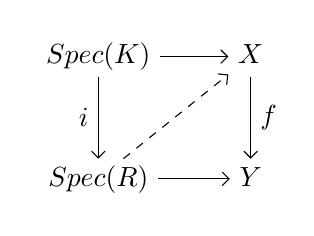
\begin{tikzpicture}[>=angle 90]
\matrix(a)[matrix of math nodes,
row sep=3em, column sep=2.5em,
text height=1.5ex, text depth=0.25ex]
{\text{Spec}(K) & X\\
\text{Spec}(R) & Y\\};
\path[->]
(a-1-1) edge node[left]{$i$} (a-2-1);
\path[->]
(a-1-1) edge (a-1-2);
\path[->,dashed]
(a-2-1) edge (a-1-2);
\path[->]
(a-1-2) edge node[right]{$f$} (a-2-2);
\path[->]
(a-2-1) edge (a-2-2);
\end{tikzpicture}
\end{figure}
%DIAGRAM1
%\sh{-10}{\box\boxA}
%\noindent
there exists a unique morphism $Spec(R) {\to} X$ making the whole
diagram commutative.
\end{theorem}

\begin{proof} \   For details and a proof see \cite{MR0463157}.
\end{proof}


\begin{proposition}{Proposition\  4.2}
The morphism $p:S_{1} {\to} S$ is proper and
hence surjective.
\end{proposition}

\begin{proof} We apply the valuative criterion of properness.  Let
  ${\eta}_{1}$ be the image in $S_{1}$ of the unique point in
  $Spec(K)$.  We select an affine patch on $S_{1}$ that intersects
  ${\eta}_{1}$ non-trivially.  We may assume that the patch is given
  by a pair of opposite Borel subgroups $(B_{0},B_{{\infty}})$ and the
  conditions $z_{1}(W_{{\alpha}},{\alpha})\ne 0$ where we are given a
  Weyl chamber $W_{{\alpha}}$ for each simple root ${\alpha}$, and
  $(z_{1}(W,{\alpha})),(z({\alpha}))$ are given representatives in
  $S^{'}(B_{{\infty}},B_{0}) \times {\AAA}^{r}$ for
  $S'(B_{{\infty}},B_{0}) \times_{T_0} {\AAA}^{{r}}$.  The condition
  $z_{1}(W_{{\alpha}},{\alpha})\ne 0$ is independent of the choice of
  representatives in $S'(B_{{\infty}},B_{0}) \times {\AAA}^{{r}}$.  On
  this affine patch the coordinate ring is generated by
  $z_{1}(W,{\alpha})/z_{1}(W_{{\alpha}},{\alpha})$ $\forall \
  (W,{\alpha})$ and
  $z(W_{{\alpha}},{\alpha})=z(\alpha)z_1(W_\alpha,\alpha)$ $\forall\
  {\alpha}$.  For each ${\alpha}$ let $W=W_{{\alpha}}^{0}$ be a choice
  of chamber for which
  $v({\varphi}^{*}(z_{1}(W,{\alpha})/z_{1}(W_{{\alpha}},{\alpha})))$
  attains its minimum as $W$ varies over chambers such that
  ${\varphi}^{*}(z_{1}(W,{\alpha})/z_{1}(W_{{\alpha}},{\alpha}))\ne
  0$.  Here $v$ is the valuation and ${\varphi}$ is the morphism
$$
{\varphi}:Spec(K) {\to} S_{1} .
$$
Now ${\eta}_{1}$ intersects the affine patch $S_{a}\ {\subseteq}\
S_{1}(B_{{\infty}},B_{0})$ whose coordinate ring is generated by
$$z_{1}(W,{\alpha})/z_{1}(W_{{\alpha}}^{0},{\alpha}),
z(W_{{\alpha}}^{0},{\alpha}).$$
 Then
$$v({\varphi}^{*}(z_{1}(W,{\alpha})/z_{1}(W_{{\alpha}}^{0},{\alpha})))
\ge  0$$ for all $(W,{\alpha})$.
 The map $S_{1} {\to} S$ is given locally by
$$
\aligned
(z_{1}(W,{\alpha})/z_{1}(W_{{\alpha}}^{0},{\alpha})),(z(W_{{\alpha}}^{0},
{\alpha})) {\to} &(z_{1}(W,{\alpha})z(W_{{\alpha}}^{0},{\alpha})/z_{1}
(W_{{\alpha}}^{0},{\alpha}))\\ =& (z(W,{\alpha})) .
\endaligned
$$
Then the assumption of a morphism $Spec(R) {\to} S$ gives
$v({\varphi}^{*}(z(W,{\alpha}))) \ge  0$.
 In particular,
$$
v({\varphi}^{*}(z(W_{{\alpha}}^{0},{\alpha})) \ge  0 .
$$
Thus the image of the coordinate ring of $S_{a}$ lies within the coordinate
ring of $R$.
 This gives a morphism from $Spec(R)$ to $S_{a}$ and hence to $S_{1}$.
 The uniqueness of the morphism is clear.
\end{proof}

\section{{Cocycles}}

The result of this section is essentially lemma 5.2 of \cite{MR701566}.  We
reproduce it here in a form more convenient for our applications.  For
every regular star $(t^{g},(B(W))^{g})$ there is a cocycle
${\sigma}(g)g^{-1}$ of $\Gal$ with values in $T(\Fb)$.  There is a
character ${\kappa}$ on $H^{1}(\Gal,T) = H^{1}(T)$ used to determine
the endoscopic group $H$ such that the integrand $f_{1}$ on $Y^{0}$ is
given by ${\pi}_{1}^{*}(f)m_{{\kappa}}(e)$ where ${\pi}_{1}^{*}(f)$ is
the pullback of a locally constant function of compact support on $G$
and $m_{{\kappa}}(e) = {\kappa}({\sigma}(g)g^{-1})$.

\addtocounter{theorem}{1} % counters are off by one in original!

\begin{proposition}   Let $R$ be the field of rational functions
of the variety of stars $S$.
 Then $m_{{\kappa}}(e)$ has an expression on a Zariski open set of the
variety of regular stars $S^{0}$
$$
m_{{\kappa}}(e) = {\kappa}(t_{{\sigma}}(e)), \qquad t_{{\sigma}}(e) \in H^{1}(T), \qquad
e \in S^{0}
$$
where for each ${\sigma} \in \Gal, t_{{\sigma}}$ belongs to
$T(R)$.
\end{proposition}

\begin{proof}     In the course of the proof we develop an expression
from which $t_{{\sigma}}$ may be calculated.
 We begin with a quasi-split group $G_{qs}$ and an inner form $G_{in}$.
 We select a maximally split Cartan subgroup $T_{qs}$ and a Borel subgroup
$B_{qs}$ both over $F$ in $G_{qs}$ with $T_{qs} {\subseteq} {B_{qs}}$.
 We select a Cartan subgroup $T_{in}$ over $F$ in $G_{in}$.
 Fix an isomorphism of $G_{qs}$ with $G_{in}$ over $\Fb$  which
carries $T_{qs}$ to $T_{in}$.
 We identify $G_{qs}$ and $G_{in}$ through this isomorphism.
 The two forms are distinguished by the actions of $\Gal$ on the
groups.
 For ${\sigma} \in \Gal$ we write ${\sigma}_{qs}$ and
${\sigma}_{in}$ for the corresponding actions on the quasi-split and inner
forms.
  For any Cartan subgroup $T$ over $F$ in $G_{in}$, select an element $h \in
G(\Fb)$ such that $T^{h}$
$= T_{qs}$.
 Write ${\sigma}_{in}(h^{-1}) = w_{{\sigma}}h^{-1}$ with $w_{{\sigma}} \in
N_{G}(T_{qs})$.
 Let $g \in T\backslash G_{in}(F)$.
 For $g$ in a Zariski open set of $G$ we can write $T^g
= T_{qs}^{h^{-1}g}\ {\subseteq}\ B_{qs}^{h^{-1}g}  =
B_{qs}^\nu$  or $h^{-1}g = tn{\nu}$ with $t \in T_{qs},
n \in N_{qs}, {\nu} \in N_{qs{\infty}}$.
 $N_{qs}$ is the unipotent radical of $B_{qs}$ and $N_{qs{\infty}}$ is the
unipotent radical of the Borel subgroup opposite to $B_{qs}$ through $T_{qs}$.
 Thus $g = htn{\nu} = (hth^{-1})hn{\nu} = t'hn{\nu}$ with $t' \in
T(\Fb)$.
 Now
$$
\sigma_{in}(g)g^{-1} = {\sigma}_{in}(t'){\sigma}_{in}(h){\sigma}_{in}(n)
{\sigma}_{in}({\nu}){\nu}^{-1}n^{-1}h^{-1}t^{\prime-1}
$$
is a cocycle in $Z^{1}(T)$ which has the same class as
$$
{\sigma}_{in}(h){\sigma}_{in}(n){\sigma}_{in}({\nu}){\nu}^{-1}n^{-1}h^{-1} .
$$
We define a twisted action ${\sigma}_{*}$ on $T_{qs}$ by
$$
{\sigma}_{*}(t) = {\sigma}_{in}(t)^{w_{{\sigma}}}, t \in T_{qs} .
$$
Then if $t_{{\sigma}}$ is a cocycle in $Z^1(T)$, we have
$$
\tau_{*}(t_{{\sigma}}^{h})t_{{\tau}}^{h} =
{\tau}_{in}(t_{{\sigma}})^{\tau_{in}(h)w_{\tau}} t_{{\tau}}^{h} =
({\tau}_{in}(t_{{\sigma}})t_{{\tau}})^{h} = (t_{{\tau}{\sigma}})^{h}.
$$
Thus there is an identification of cocycles in $T$ and twisted cocycles in
$T_{qs}$.
$$
h^{-1}{\sigma}_{in}(h){\sigma}_{in}(n){\sigma}_{in}({\nu}){\nu}^{-1}n^{-1} =
$$

$$
w_{{\sigma}}^{-1}{\sigma}_{in}(n){\sigma}_{in}({\nu}){\nu}^{-1}n^{-1}
$$
is then a cocycle in $T_{qs}$ with this twisted action.
 Call this cocycle $T_{{\sigma}}$.
$$
T_{{\sigma}}^{w_\sigma^{-1}} =
{\sigma}_{in}(n){\sigma}_{in}({\nu}){\nu}^{-1}n^{-1}w_{{\sigma}}^{-1}.
$$
Since $G_{qs}$ and $G_{in}$ are inner forms, we may write
$$
{\sigma}_{in}(g) = {\bold {ad}}\ A_{{\sigma}}^{-1}({\sigma}_{qs}(g)),
$$
where ${\sigma} {\to} A_{{\sigma}}$ is a cocycle
with values in $N_{G_{qs}}(T_{qs})_{adj}$, the image of the normalizer
in the adjoint group,
with respect to the action ${\sigma}_{qs}$.
Now
$$
\aligned
T_{{\sigma}}^{w_\sigma^{-1}} &= A_{{\sigma}}^{-1}{\sigma}_{qs}(n)
{\sigma}_{qs}({\nu})A_{{\sigma}}{\nu}^{-1}n^{-1}w_{{\sigma}}^{-1} \\
T_\sigma^{w_\sigma^{-1}A_\sigma^{-1}} & = {\sigma}_{qs}(n)
{\sigma}_{qs}({\nu})A_{{\sigma}}{\nu}^{-1}n^{-1}w_{{\sigma}}^{-1}
A_{{\sigma}}^{-1}
\endaligned
$$

\begin{eqn}  %{Equation 5.3}
$A_{{\sigma}}{\nu}^{-1}n^{-1}
w_{{\sigma}}^{-1}A_{{\sigma}}^{-1} \in
N_{{\infty}qs}N_{qs}T_{{\sigma}}^{w_\sigma^{-1}A_\sigma^{-1}}$ .
\end{eqn}

These last two equations are the fundamental relation from which the
function $m_{{\kappa}}(e)$ can be deduced for all reductive groups.
The equation 5.3 determines $T_{{\sigma}}$ as a rational function of
the coefficients
of $$A_{{\sigma}}{\nu}^{-1}n^{-1}w_{{\sigma}}^{-1}A_{{\sigma}}^{-1}.$$
\end{proof}

The cocycle $w_{{\sigma}}$ measures the extent to which $T_{in}$ and
$T$ are not isomorphic over $F$, and $A_{{\sigma}}^{-1}$ measures the
extent to which $T_{in}$ and $T_{qs}$ are not isomorphic over $F$.  We
give a few applications of this formula that will be useful in chapter
VII when we carry out the transfer of the subregular germ for certain
groups.

\medskip

\begin{corollary}{Corollary\ 5.4}\   Suppose that $A_{{\sigma}} = 1$, $B_{0} = B_{qs}$,
$T_{0} = T_{qs}$, and that $w_{{\sigma}}$ is a simple reflection corresponding
to the root ${\alpha}$.
 Then $t_{0}T_{{\sigma}} = (z(W_{+},{\alpha}))^{\alpha^v}$  for some
element $t_{0} \in T_{qs}(\Fb)$ independent of the regular star.
\end{corollary}

\begin{proof}     Equation 5.3 gives $n^{-1}w_{{\sigma}}^{-1} \in
N_{qs{\infty}}N_{qs}T_{{\sigma}}^{w_\sigma^{-1}}$.
$w_{{\sigma}}^{-1}$ differs from ${\sigma}_{{\alpha}}$ by an element of
$T_{qs}$ independent of the star.
 Here ${\sigma}_{{\alpha}}$ is the image in $G$ of the reflection
$
\begin{pmatrix} \prelax
%\format \r\quad & \r \\
0 & 1 \\ -1 & 0 \end{pmatrix}
$
in $G_{{\alpha}}$ where $G_{{\alpha}}$ is the rank one subgroup corresponding
to the root ${\alpha}$.
 We combine this element with $T_{{\sigma}}$ and write
$n^{-1}{\sigma}_{{\alpha}} \in
N_{qs{\infty}}N_{qs}(t_{0}T_{{\sigma}})^{\sigma_\alpha}.$  Now by the $2$ by $2$ matrix calculation

{\bigskip}

$$
{\begin{pmatrix}
%\prelax  \format \c \quad & \c \\
1 & -n_\alpha \\ 0 & 1 \end{pmatrix}}
{\begin{pmatrix}
%\prelax  \format \r \quad & \r \\
0\  & 1 \\ -1\  & 0 \end{pmatrix}}\ =\
{\begin{pmatrix}
%\prelax  \format \r \quad & \r \\
n_\alpha & 1 \\ -1{\phantom{n}} & 0 \end{pmatrix}}\ =\
{\begin{pmatrix}
%\prelax   \format \c \quad & \c \\
1 & 0 \\ -1/n_\alpha & 1 \end{pmatrix}}
{\begin{pmatrix}
%\prelax  \format \l \quad & \c \\
n_\alpha & 1 \\ 0 & 1/n_\alpha \end{pmatrix}}\ =
$$
$$
{\begin{pmatrix}
%\prelax  \format \c \quad & \c \\
1 & 0 \\ -1/n_\alpha & 1 \end{pmatrix}}
{\begin{pmatrix}
%\prelax  \format \l \quad & \l \\
1 & n_\alpha \\ 0 & 1 \end{pmatrix}}
{\begin{pmatrix}
%\prelax  \format \l \quad & \c \\
 n_\alpha & 0 \\ 0 & 1/n_\alpha \end{pmatrix}}.
$$

\begin{eqn} % {Equation\ 5.5}
$$\epsilon_\alpha(-n_{{\alpha}})
{\sigma}_{{\alpha}} = {\epsilon}_{-{\alpha}}(-1/n_{{\alpha}})
{\epsilon}_{{\alpha}}(n_{{\alpha}})n_{{\alpha}}^{\alpha^v}$$
where $\epsilon_{\pm\alpha}(X) = \exp(x X_{\pm\alpha})$.
\end{eqn}

\noindent
From this it follows that $n^{-1}{\sigma}_{{\alpha}} \in
N_{{\infty}}N_{0}n_{{\alpha}}^{\alpha^v}.$  Also
$$
B(W({\sigma}_{{\alpha}})) = B_{0}^{\exp(z(W_{+},{\alpha})X_{-{\alpha}})\nu}
$$
and $B(W({\sigma}_{{\alpha}})) = B_{0}^{\sigma_\alpha h^{-1}g}
= B_{0}^{\sigma_\alpha n{\nu}}.$  From this it follows that
$$
B_{0}{\sigma}_{{\alpha}}n = B_{0}\exp(z(W_{+},{\alpha})X_{-{\alpha}}) ,
$$
and by (5.5) it follows that $n_{{\alpha}} = 1/z(W_{+},{\alpha})$.
 The result follows from the relations $n_{{\alpha}} = 1/z(W_{+},{\alpha})$
and ${\sigma}_{{\alpha}}({\alpha}^{v}) = -{\alpha}^{v}$.
\end{proof}

\begin{remark}[5.6]    When $A_{{\sigma}} = 1$, for the classical
groups we can recover $T_{{\sigma}}$ from the equation $$n^{-1}w_{{\sigma}}^{-1}
\in N_{qs{\infty}}N_{qs}T_{{\sigma}}^{w_\sigma^{-1}}$$  by computing
the principal minors of both sides noting that the principal minors of any
matrix in $N_{qs{\infty}}N_{qs}$ are equal to one provided we choose a
representation such that $B_{qs}$ is upper triangular and $T_{qs}$ is diagonal.
\end{remark}

\begin{corollary}{Corollary 5.7}    Suppose that $A_{{\sigma}}$ is a simple reflection
corresponding to a root ${\alpha}$, and ${\nu} =
{\epsilon}_{-{\alpha}}({\xi})^{{\alpha}}{\nu}$ with $^{{\alpha}}{\nu} \in
N_{{\alpha}}$.
 Then $T_{{\sigma}}$ is determined by the condition
$$
\sigma_{{\alpha}}{\epsilon}_{-{\alpha}}(-{\xi})n^{-1}w_{{\sigma}}^{-1}
{\sigma}_{{\alpha}}^{-1} \in
N_{qs{\infty}}N_{qs}(t_{1}T_{{\sigma}})^{w_\sigma^{-1}{\sigma}_{{\alpha}}^{-1}}
$$
where $t_{1} \in T_{qs}$ is independent of the star.
\end{corollary}

\begin{proof}   This follows immediately from (5.3) if we note that
$$A_{{\sigma}}\ {}^{{\alpha}}{\nu}^{-1}A_{{\sigma}}^{-1} \in N_{qs{\infty}}.$$
\end{proof}


\section{{The\ Data}}

   In this section we prove that the Igusa data exists for any reductive
group, and show how to associate a unipotent conjugacy class to each divisor.
 Let $G$ be a connected reductive group.
 We have morphisms ${\varphi}, {\pi}_{1}$, and ${\xi}$.
\begin{figure}[htb]
\centering
\begin{tikzpicture}[>=angle 90]
\matrix(a)[matrix of math nodes,
row sep=3em, column sep=2.5em,
text height=1.5ex, text depth=0.25ex]
{T^0\times T\backslash G& X_1 & G\\
 &T&\\};
\path[->]
(a-1-1) edge (a-2-2);
\path[->]
(a-1-1) edge node[above]{$\phi$} (a-1-2);
\path[->]
(a-1-2) edge node[above]{$\pi_1$} (a-1-3);
\path[->]
(a-1-2) edge node[right]{$\xi$} (a-2-2);
\end{tikzpicture}
\end{figure}

%\vfill
%DIAGRAM2
%\sh{-5}{\box\boxB}
%\vskip .2in

\noindent
The maps are $G$-equivariant maps provided $G$ acts on $G$ by ad, on $T^{0}
\times T\backslash G$ by translation on the second factor, and trivially on $T$.
 The maps ${\varphi}$, ${\xi}$ and ${\pi}_{1}$ are defined over $F$.
${\xi\circ\varphi}$ is projection on the first factor.
 So the diagram above commutes.
${\pi}_{1}({\varphi}(t,g)) = {\pi}_{1}(t^{g},({\BB}(W))^{g}) = t^{g} \in G$.
 The map ${\pi}_{1}$ is proper.

   Now let ${\Gamma}$ be a curve in $T$.
 The curve ${\Gamma}$ is assumed to be a smooth curve which passes through the
identity of $T$ where its tangent is regular in the sense that it does not
lie in a hyperplane defined by a root and which contains no other singular
point.
 Let ${\Gamma}^{0}={\Gamma}\backslash \{0\}, Y_{1}^{0}={\xi}^{-1}({\Gamma}^{0})$,
and let $Y_{1}$ be its closure in $X_{1}$.
 $G$ then acts on $Y_{1}$ since ${\xi}$ is a $G$-morphism.  We also let $1$
 denote the element of $\Gamma\setminus\Gamma^0$.
 We have

\begin{figure}[htb]
\centering
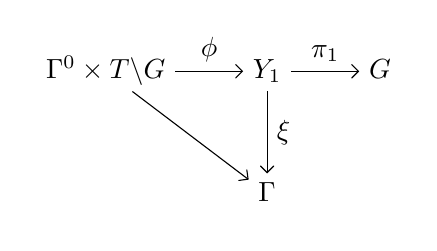
\begin{tikzpicture}[>=angle 90]
\matrix(a)[matrix of math nodes,
row sep=3em, column sep=2.5em,
text height=1.5ex, text depth=0.25ex]
{\Gamma^0\times T\backslash G& Y_1 & G\\
 &\Gamma&\\};
\path[->]
(a-1-1) edge (a-2-2);
\path[->]
(a-1-1) edge node[above]{$\phi$} (a-1-2);
\path[->]
(a-1-2) edge node[above]{$\pi_1$} (a-1-3);
\path[->]
(a-1-2) edge node[right]{$\xi$} (a-2-2);
\end{tikzpicture}
\end{figure}

%\vfill
%DIAGRAM3
%\sh{-5}{\box\boxC}
%\medskip


\noindent
All morphisms are $G$-morphisms, and defined over $F$ provided ${\Gamma}$ is
defined over $F$.

   Replace $Y_{1}$ by a desingularization $Y_{{\Gamma}}$.
 The desingularization may be chosen to be $G$-equivariant, and the
irreducible components of ${\xi}=1$ may be assumed to have normal crossings
\cite{MR0102519}.
 Thus $G$ acts on $Y_{{\Gamma}}$ and all morphisms are $G$-morphisms.

   ${\xi}^{-1}(1) {\subseteq} Y_{{\Gamma}}$ breaks up into a finite number
of irreducible components.
 The expression {\it divisor}  refers in this text to them.
 Conjugacy classes are taken to mean stable conjugacy classes unless indicated
otherwise.
\vskip .2in

\begin{lemma}{Lemma 6.1}  Let $E$ be a divisor in $Y_{{\Gamma}}$.
 There is a unique unipotent conjugacy class $O$ in $G$ such that
${\pi}_{1}(E)$ equals the closure of $O$ in $G$.
\end{lemma}

\begin{proof}   Since $G$ is connected, $G$ fixes each divisor.
 ${\pi}_{1}(E)$ is also closed (by properness), irreducible, and $G$-invariant.
 So ${\pi}_{1}(E)$ is a union of conjugacy classes.
 If ${\xi}(x)=1$ then ${\pi}_{1}(x)$ lies in a Borel subgroup $B$ and
${\pi}_{1}(x)$ modulo $N$ is $1$.
 Thus ${\pi}_{1}(x)$ lies in $N$ and is consequently unipotent.
 Call the unipotent classes in ${\pi}_{1}(E) \ \ O_{1},\ldots ,O_{j}$ and their
closures $X_{1},\ldots ,X_{j}$.
 ${\pi}_{1}(E)=X_{i}$ for some $i$ by irreducibility.
 $X_{i}$ determines the unipotent class uniquely for the classes in the
closure are of strictly lower dimension.
\end{proof}

   If $E$ is associated with the unipotent class $O$, call $E$ an
{\it $O$-divisor}.  Similarly call $E$ a {\it regular} or {\it subregular }
divisor  if the unipotent class associated to $E$ is regular or subregular.
\vskip .2in

\begin{remark}{Remark\ 6.2}   Let $u,u' \in O$, then $u^{g}=u'$ for some $g$
and $Y_{{\Gamma}} {\to} Y_{{\Gamma}}$ gives an isomorphism of the fibre
$E(u)$ over $u$ with the fibre $E(u')$ over $u'$ whenever $E$ is an $O$-divisor.
 This isomorphism is defined over $F$ if $u,u'$ lie in the same adjoint
conjugacy class.
 By an adjoint conjugacy, we mean $F$-conjugacy in $G_{adj}(F)$.
 See \cite{MR683003} for details.
 By letting $u=u'$ we obtain an action of $C_{G}(u)$ on $E(u)$.
 \end{remark}

\begin{theorem}{Theorem 6.3}  Let $G$ be reductive.
 There exists a variety $Y_{{\Gamma}}$ proper over $Y_{1}$ such that the
conditions for Igusa data are met.
\end{theorem}

\begin{proof}   By blowing up $G$-equivariantly if necessary we may assume
the variety $\lambda=0$ (i.e. $\xi=1$) is
the union of divisors with normal crossings.
 The only condition that has not been verified in \cite{MR701566} is that $f$ locally
has the form ${\gamma}{\kappa}_{1}({\mu}_{1})\ldots {\kappa}_{n}({\mu}_{n})$
where ${\mu}_{1},\ldots ,{\mu}_{n}$ are local $F$-coordinates on
$Y_{{\Gamma}}$ at a point $p$, and ${\kappa}_{1},\ldots ,{\kappa}_{n}$ are
characters of $F^{\times}$.
 The function ${\gamma}$ must be locally constant at $p$ and if
${\kappa}_{i}$ is not the trivial character, ${\mu}_{i}=0$ must define a
divisor passing through $p$.

   Fix a basis ${\Lambda}$ for the characters of $T$.
 By (5.2), if ${\chi} \in {\Lambda}$ then ${\chi}(t_{{\sigma}}) \in R$
the field of rational functions on $S$.
 Working with a finite extension $K$ of $F$ and pulling ${\chi}(t_{{\sigma}})$
back to the field of functions on $Y_{{\Gamma}}$ we obtain finitely many prime
divisors determined by the Weil divisors of
${\chi}(t_{{\sigma}})$ for all ${\chi} \in {\Lambda}, {\sigma} \in
\GalK$.
 By blowing up if necessary, we may assume that these prime divisors
together with the prime divisors determined by ${\lambda}=0$ all have normal
crossings.
 Let $\langle E\rangle$ be the set of prime divisors.
 Again blowing up if necessary, we may assume that a prime divisor of $\langle E\rangle$
has $F$-rational points if and only if it is defined over $F$.
 In the neighborhood on the $p$-adic manifold of an $F$-rational point $p$
we may write
$$
{\chi}(t_{{\sigma}}) = {\alpha}{\mu}_{1}^{a_1} \ldots {\mu}_{n}^{a_n}
$$
where $a_{1},\ldots ,a_{n},{\alpha}$ depend on ${\chi}$ and ${\sigma}$.
 We may assume that ${\mu}_{1},\ldots ,{\mu}_{n}$ are local $p$-adic
coordinates at $p$ and that ${\alpha}$ is regular and invertible at $p$.
 It follows that $t_{{\sigma}}$ has the form
$$
t_{{\sigma}}: {\sigma} {\to}
{\mu}_{1}^{{\beta}_{1{\sigma}}} \ldots {\mu}_{n}^{{\beta}_{n{\sigma}}}
\overline{t}_{{\sigma}}
$$
for some cocharacters
${\beta}_{1{\sigma}},\ldots ,{\beta}_{n{\sigma}}$ and
$\overline{t}_{{\sigma}}$, where
$\overline{t}_{{\sigma}}$ is regular at $p$.
 Since $t_{{\sigma}}$ is a cocycle ${\tau}(t_{{\sigma}})t_{{\tau}} =
t_{{\tau}{\sigma}}$, that is
$$
\mu_{1}^{\tau({\beta}_{1{\sigma}})} \ldots
{\mu}_{n}^{\tau({\beta}_{n{\sigma}})}
{\tau}(\overline{t}_{{\sigma}}){\mu}_{1}^{{\beta}_{1{\tau}}} \ldots
{\mu}_{n}^{{\beta}_{n{\tau}}} \overline{t}_{{\tau}} =
{\mu}_{1}^{{\beta}_{1{\tau}{\sigma}}}\ldots {\mu}_{n}^{{\beta}_{n{\tau}{\sigma}}}
\overline{t}_{{\tau}{\sigma}}.
$$

\noindent
Rearranging:
$$
\mu_{1}^{[{\tau}({\beta}_{1{\sigma}})+{\beta}_{1{\tau}}-
{\beta}_{1{\tau}{\sigma}}]} \ldots
{\mu}_{n}^{[{\tau}({\beta}_{n{\sigma}})+{\beta}_{n{\tau}}-{\beta}_{n{\tau}{\sigma}}]}
= \overline{t}_{{\tau}{\sigma}} \overline{t}_{{\tau}}^{-1}
{\tau}(\overline{t}_{{\sigma}}^{-1}).
$$
The right hand side is regular at $p$, so the left hand side must be as well.
 This forces
$$
{\tau}({\beta}_{i{\sigma}})+{\beta}_{i{\tau}} = {\beta}_{i{\tau}{\sigma}}
$$
for all $i$.
 Thus ${\sigma} {\to} {\mu}_{i}^{{\beta}_{i{\sigma}}}$  is a cocycle
${\ \forall \ } i$, and ${\sigma} {\to} \overline{t}_{{\sigma}}$
is as well.
 We then define the character ${\kappa}_{i}$ on $F^{x}$ by
${\kappa}_{i}({\mu}) = {\kappa}({\mu}^{\beta_{i{\sigma}}})$
where ${\kappa}$ is the
character on $H^{1}(T)$ defining the endoscopic group.
 This shows that the function $f_{1}$ has the correct form.

   There is one last point to verify.
 It  must be possible to choose the coordinates ${\mu}_{1},\ldots, {\mu}_{n}$
in such a way that if ${\mu}_{i}=0$ does not define a divisor then
${\kappa}_{i}=1$.
 Since the divisors have normal crossings, we may assume that if $E$ is a
divisor then it is given locally by ${\mu}_{i}=0$ for some $i$.
 But then if ${\mu}_{j}=0$ does not define a divisor, points of ${\mu}_{j}=0,
\ {\mu}_{i}\ne 0 \ i\ne j$ are regular stars.
 The result then follows from the fact that $m_{{\kappa}}(e)$ is locally
constant on the regular stars (cf. \cite{MR701566}).
\end{proof}

%%%% end of athis.tex

%%%% start of bthis.tex


\chapter{Coordinates and Coordinate Relations}

%\showthe\topskip
%\showthe\hoffset\showthe\voffset
%\tracingoutput=2
%\showboxdepth=2



\section{The\ Coordinates\ $x(W,\beta)$ }

Before deriving any concrete results from the variety $Y_{{\Gamma}}$ it will
be necessary to develop coordinates charts on the variety.
 This section introduces coordinates $x(W,{\beta})$ indexed by Weyl chambers
$W$ and positive roots ${\beta}$.
 They can be described as follows.
 Consider a point $p \in X_{1} {\subseteq} G \times S_{1}$.
 Then locally $p \in B_{0} \times S_{1}(B_{{\infty}}) \tilde{\to}  B_{0}
\times S_{1}(B_{{\infty}},B_{0}) \times N_{{\infty}}._{ }$ Write
$p = (b,e,{\nu})_{.}$  For each simple root ${\alpha}$ fix root vectors
$X_{{\alpha}}$ and $X_{-{\alpha}}$ for $T_{0} = B_{0} {\cap} B_{{\infty}}$
in the Lie algebra of $G$ such that $[X_{{\alpha},}X_{-{\alpha}}] =
H_{{\alpha}}$ with ${\alpha}(H_{{\alpha}})=2$.
 Fix an ordering on the positive roots then write $b \in B_{0}$  as
$$
t \prod  \exp(x_{{\beta}}X_{{\beta}})\qquad  ({\text{ordered}})
$$
with $t \in T_{0}$.
 To fix a convention, we agree that lower elements in the ordering appear
to the left in the product.
 Then $t$ and $x_{{\beta}} = x_{{\beta}}(b)$ are coordinates for $b$.
  If $e = (B_{0}^{n_w})$, then $b^{n_w^{-1}} \in B_{0}$ for all $W$.
 Define $x(W,{\beta})$ to be $x_{{\beta}}(b^{n_w^{-1}})$.
 This definition depends on the order of the product.
 In concrete situations the order will always be specified.
 Notice, however, that $x(W,{\alpha})$ for ${\alpha}$ simple is independent
of the order.

\section{The\ Coordinates\ $w({\beta})$ }

This section defines a set of coordinates $w({\beta})$ on certain open
patches $Y''(B_{{\infty}})$ of the open set $Y''$ indexed by positive non-simple
roots ${\beta}$.
 These coordinates will prove to be extremely useful on this open set.
 With them it will be possible to study the structure of those divisors in
$Y_{{\Gamma}}$ whose image in $Y_{1}$ meets $Y''$.
 The coordinates are easy to define; but it must be checked that they are
truly regular coordinates on $Y''$.
 These verifications will be made in section $3$.

   Select the Borel subgroup $B_{{\infty}}$ to be opposite to
${\BB}(W_{+})$.
 We work on the coordinate patch $Y^{0}(B_{{\infty}})$.
 The restriction that $B_{{\infty}}$ lie opposite ${\BB}(W_{+})$ is not a
serious restriction.
 Although patches of this sort do not cover $Y^{0}$, translates of these
patches by elements of $G$ do cover $Y^{0}$ so that no structural information
is lost by making the assumption that $B_{{\infty}}$ is opposite
${\BB}(W_{+})$.
 We have maps:
$$
T^{0} \times T\backslash G {\to} X^{0}
$$
$$
(t,g) {\to} (t^{g},({\BB}(W)^{g})) .
$$
On $Y^{0}(B_{{\infty}})$ we have ${\BB}(W_{+})^{g} =
{\BB}(W_{+})^{{\nu}}$ for some ${\nu} \in N_{{\infty}}$, the unipotent
radical of $B_{{\infty}}$.
 Thus $g=t_{0}n{\nu}$ for uniquely defined $t_{0} \in T_{0}, n \in N_{0}$,
and ${\nu} \in N_{{\infty}}$ where $N_{0}$ is the unipotent radical of
${\BB}(W_{+})$.
 Then on $Y^{0}(B_{{\infty}},{\BB}(W_{+})) \times N_{{\infty}}\
{\widetilde{\to}}\  Y^{0}(B_{{\infty}})$, $(t^{g},({\BB}(W)^{g}))$ equals
$(t^{n},({\BB}(W)^{n}))^{{\nu}}$.
 Define $y({\beta})$ by $t^{n} = t \prod \exp(y({\beta})X_{{\beta}})$.
 The definition of $y({\beta})$ depends on the order of the product.
 Suppose ${\beta} = \sum m({\alpha}){\alpha}$.
 Then define $w({\beta})$ by
$$
w({\beta}) = y({\beta})
\prod z({\alpha})^{m({\alpha})}/{\lambda}
$$
where $z({\alpha})$ is defined to be the quantity which makes $w({\alpha}) = 1$
for ${\alpha}$ simple.
 That is, $z({\alpha}) = {\lambda}/y({\alpha})$.

   This gives the definition of $w({\beta})$ on an open set of
$Y_{1}(B_{{\infty}})$.
 This definition depends on the order the product defining $y({\beta})$.
 In applications the order must be specified.


   It must be checked that $w({\beta})$ extends to a regular coordinate on
$Y''(B_{{\infty}})$.
 Formulas will be given relating the coordinates $w({\beta})$ to $t, n$, and
the coordinates $$z_{1}(W,{\alpha}) =^{def}
z(W,{\alpha})/z({\alpha}).$$
 These topics are treated in the next few sections.

\section{The\ Extension\ of\ $w({\beta})\ to\ Y''$}

   This section shows that the coordinates $w({\beta})$ are regular on
$Y''(B_{{\infty}})$.
 Before proving the result I state a well known lemma that will be needed in
the proof.

\begin{lemma}{Lemma 3.1}   Let ${\alpha}$ and ${\beta}$ be positive roots, and
let $\Psi$
 be the set of roots of the form $r{\alpha} + s{\beta}$ \ ($r,s$ positive integers).
  Fix vectors $X_{{\gamma}}$.
 Then the commutator $(\exp(xX_{{\alpha}}),\exp(yX_{{\beta}}))$ equals
$\prod \exp(c_{{\alpha}{\beta}{\gamma}}x^{r}y^{s}X_{{\gamma}})$, where the
product is taken over all ${\gamma}=r{\alpha}+s{\beta} \in \Psi$
(in some fixed order) and where $c_{{\alpha}{\beta}{\gamma}}$ are constants
independent of $x$ and $y$.
\end{lemma}

\begin{proof}    \cite{MR0396773}*{\S32.5}.
\end{proof}

{\medskip}

The following result is independent of the order selected on the roots to
define $y({\beta})$.

\begin{lemma}{Lemma 3.2}   The coordinates $w({\beta})$ are regular on
$Y''(B_{{\infty}})$.
 The coordinates $w({\beta})$ may be expressed as a function of
$\{t,(z(\alpha)),(z_{1}(W,\alpha))\}$.\  As such they are actually
independent of the coordinates $\{z(\alpha)\}$.
\end{lemma}


   In the course of the proof we will prove a second lemma.
 Write for any element $n \in N_{0}$ and $t \in T$
$$
\aligned
n & = \prod \exp(n_{{\beta}}X_\beta)  \\
t^n &= t\prod \exp(y({\beta})X_\beta)
\endaligned  \qquad
\aligned (\text{ordered})  \\
(\text{ordered})
\endaligned
$$

\noindent
Any order on the roots may be selected, but it must be the same for both products.
 Solve these equations for $y({\beta})$ in terms of the variables
$\{n_\alpha,\alpha^{-1}(t)\}$\ ($\alpha$ positive).   We obtain an
expression of the form:
$$
y(\beta) = \sum  c_{\beta_1\ldots \beta_n} (t)n_{\beta_1} n_{\beta_2}\ldots
n_{\beta_n}
$$
where the sum ranges over the set ${\beta}_{1} + {\beta}_{2} +\ldots +
{\beta}_{n} = {\beta}$.

\begin{lemma}{Lemma 3.3}   $c_{\beta_1\ldots \beta_n}(t)$ is a sum of terms
of the form $(1-{\gamma}_{1}^{-1}(t)){\gamma}_{2}(t)$ where
${\gamma}_{1}$ is a root and ${\gamma}_{2}$ is a linear combination of roots.
 Also $c_{{\beta}}(t)$ equals $(1-{\beta}^{-1}(t))$.
 In particular $y({\alpha})=(1-{\alpha}^{-1})n_{{\alpha}}$ for ${\alpha}$
simple.
\end{lemma}

\begin{proof}    The positive roots can be numbered according to the
ordering on them: ${\alpha}_{1},\ldots ,{\alpha}_{k}$ so that
$$
n = \prod {\epsilon}_{i}(n_{i})\  {\text{with}}\  {\epsilon}_{i} =
\epsilon_{\alpha_i}, n_i = n_{\alpha_i},\  {\text{and}}\
\epsilon_\alpha(x) = \exp(xX_\alpha) .
$$
Then $t^{-1}n^{-1}tn$ is given by
$$
{\epsilon}_{k}(-{\alpha}_{k}^{-1}(t)n_{k})\ldots
{\epsilon}_{1}(-{\alpha}_{1}^{-1}(t)n_{1}){\epsilon}_{1}(n_{1})\ldots
{\epsilon}_{k}(n_{k}) .
$$
The innermost terms combine to give ${\epsilon}_{1}((1-{\alpha}_{1}^{-1}
(t))n_{1})$.
 This term can be pulled through the product to the left.
 By (3.1), doing so will only add terms whose dependence on $T$ has the
form $(1-{\alpha}_{1}^{-1}(t)){\gamma}(t)$ where ${\gamma}$ lies in the
coordinate ring of $T$.
 By repeatedly pulling out the innermost term of the product, we arrive at
the result.
 It is clear from this procedure that $c_{{\beta}}(t)$ equals
$(1-{\beta}^{-1}(t))$.
 This completes the proof of lemma 3.3.
\end{proof}
\vskip .2in

We continue with the proof of (3.2).
 $n_{{\beta}}$ is a function on $Y^{0}(B_{{\infty}}) {\subseteq} G \times
S^{0}(B_{{\infty}},B_{0}) \times N_{{\infty}}$.
 It actually depends only on the second factor so that $n_{{\beta}}$ is a
function on $S^{0}(B_{{\infty}},B_{0})$.
 By the inclusion $$S^{0}(B_{{\infty}},B_{0}) {\subseteq} S''(B_{{\infty}},B_{0}),  $$
$n_{{\beta}}\prod
z({\alpha})^{m({\alpha})}$ is then a rational function on
$S''(B_{{\infty}},B_{0})$.
\vskip .2in

\begin{lemma}{Lemma 3.4}   $n_{{\beta}} \prod z({\alpha})^{m({\alpha})}$
considered as a rational function on
$S''(B_{{\infty}},B_{0})$ is regular and depends only on the coordinates
$$z_{1}(W,{\alpha}) = z(W,{\alpha})/z({\alpha})$$ and not on the coordinates
$z({\alpha})$.
\end{lemma}

\begin{remark*}  %{Remark}
This lemma will complete the proof of lemma 3.2, for
$$
w({\beta}) = y({\beta})(\prod z({\alpha})^{m(\alpha)})/{\lambda} =
\sum [c_{\beta_1\ldots \beta_n} (t)/{\lambda}]
\prod (n_{\beta_i} \prod z({\alpha})^{m_i(\alpha)})
$$
where ${\beta}_{i}=\sum m_{i}({\alpha}){\alpha}$ and
$c_{\beta_1\ldots \beta_n} (t)/{\lambda}$ is regular at ${\lambda} = 0$.
\end{remark*}

\begin{proof}[Proof\ of\ 3.4]    The matrices $n_{w}$ depend only on $(z(W,{\alpha}))$.
 Since $z(W,{\alpha}) = z({\alpha})z_{1}(W,{\alpha})$ they depend on
$z_1(W,{\alpha})$ and $z({\alpha})$.
 Recall that the matrix $n_{w}$ in $N_{{\infty}}$ is defined by the condition
${\BB}(W)^{g\nu^{-1}} = B_{0}^{n_w}.$
On our
coordinate patch $$B_{0} = {\BB}(W_{+})={\BB}$$ and $g = t_{0}n{\nu}$.
 The condition $${\BB}(W)^n  =
{\BB}^{n_w} \ \forall \ W$$ allows one to
express $n_{{\beta}}$ in terms of the variables
$\{z({\alpha}),z_{1}(w,\alpha)\}$.   The torus $T_{0}$ acts on the points
$e = ({\BB}(W)^{n\nu}) =
({\BB}^{n_w\nu})$ by $$e {\to} e^{t_0}  = ({\BB}(W)^{n\nu t_0}) =
({\BB}^{n_w\nu t_0}),$$ $t_{0} \in T_{0}(\Fb)$.
The coordinates of $e^{t_0}  = ({\BB}(W)^{n'{\nu}'}) =
({\BB}^{n_{w}'{\nu}'})$ are clearly given by ${\nu}' =
adt_0^{-1}({\nu})$, $n' = adt_0^{-1}(n)$, $n'_{w} =
adt_0^{-1}(n_{w})$, or $$n'_{{\beta}} = {\beta}(t_0^{-1})n_{{\beta}},\quad
z'(W,{\alpha}) = {\alpha}^{-1}(t_0^{-1})z(W,{\alpha}) =
{\alpha}(t_0)z(W,{\alpha}).$$

   For any choices of $z({\alpha}) \in \Fb^{\times}$, $t_0$ can be selected
to give ${\alpha}(t_0^{-1}) = z({\alpha})$ for all ${\alpha}$.
 Then ${\beta}(t_0^{-1}) = \prod z({\alpha})^{m({\alpha})}$  if ${\beta} =
\sum m({\alpha}){\alpha}$.
 Write $\underline{n}_{{\beta}}$ for the rational function of the variables
$(z({\alpha})),(z_1(W,{\alpha}))$ described above, $n_{{\beta}}$ for the
value of $\underline{n}_{{\beta}}$ at $(z({\alpha})),(z_{1}(W,{\alpha}))$ and
$n_{{\beta}}'$ for the value of $\underline{n} _{{\beta}}$ at
$(1^r,(z'(W,{\alpha}))) =
(1^r,({\alpha}(t_{0})z(W,{\alpha}))) = (1^r,
(z({\alpha})^{-1}z(W,{\alpha}))) = (1^r,(z_{1}(W,{\alpha})))$.
 $(1^r$ denotes the vector in ${\AAA}^r$ whose components
are all equal to one.)  This gives the needed independence:
$$
\underline{n}_{{\beta}}(1^r,(z_{1}(W,{\alpha}))) =
\prod z({\alpha})^{m({\alpha})}\underline{n}_{{\beta}}((z({\alpha})),
(z_{1}(W,{\alpha})))
$$
for
$$
\aligned
\underline{n}_{{\beta}}(1^r,(z_{1}(W,{\alpha})))/(\prod
z({\alpha})^{m({\alpha})}) &= n'_{{\beta}}/(\prod z({\alpha})^{m({\alpha})}) \\
&= {\beta}(t_0)n'_\beta \\
&= n_\beta \\
&= \underline{n}_{{\beta}}((z({\alpha})),(z_{1}(W,{\alpha}))).
\endaligned
$$

%\medpagebreak

Finally, we check that $n_{{\beta}} \prod z({\alpha})^{m({\alpha})}$
is regular on $S^{\prime\prime}(B_{{\infty}},B_{0})$.
The point
\newline
$((z_{1}(W,{\alpha})),{\nu}) \in S^{0}(B_{{\infty}},B_{0})
\times N_{{\infty}}$ describes a regular star $e$.
 Since it is a regular star there is a unique $n_0 \in N_{0}$ such that
$e = ({\BB}(W)^{n_0\nu})$.
 It follows that the coefficients $n_{0\beta}$ of $n_0$ are regular
functions of $(z_{1}(W,{\alpha}))$.
 But $n_{0\beta}(z_{1}(W,{\alpha})) = \underline{n}_{{\beta}}(1^r,
(z_{1}(W,{\alpha}))) = n_{{\beta}} \prod z({\alpha})^{m({\alpha})}$
so that $n_{{\beta}} \prod z({\alpha})^{m({\alpha})}$ too is regular.
 The proofs of the lemmas 3.2 and 3.4 are now complete.
 \end{proof}

\section{The\ Coordinate\ Ring}

   For $(g,(B(W)))$ in $Y''(B_{{\infty}})$ write $(g,(B(W))) =
(b,(B_{0}^{n_w}))^\nu$  where $b \in B_{0}={\BB}(W_{+})$.
 For the next proposition it is important to work on the affine patch
$Y^{\prime\prime}(B_{{\infty}})$.  We let $\lambda$ denote the pullback
to $Y_\Gamma$ (or any related variety) of a local parameter on $\Gamma$.

\medpagebreak

\begin{proposition}{Proposition  4.1}
\begin{enumerate}[label={\alph*)}]
\item The subring of the coordinate ring of $Y^{\prime\prime}(B_\infty,\BB(W_+)$
generated by $\lambda$ and $\{z_{1}(W,{\alpha}): \ \forall\
(W,\alpha)\}$\ is contained in the subring generated by the
coordinates $\{w({\gamma}) : {\gamma} > 0$, ${\gamma}$ not simple$\}$
and\ ${\lambda}$.
\item The coefficients of $b, \{z({\alpha}):{\alpha}\ {\text{simple}}\}$,
${\lambda}$,
and $\{w({\gamma}):{\gamma}$ positive but not simple$\}$\ are regular and together generate
the coordinate ring of \hfil\break $Y''(B_{{\infty}},{\BB}(W_{+}))$.
\end{enumerate}
\end{proposition}

\begin{proof}      Let $R$ be the ring generated by ${\lambda}$ and
$\{w(\gamma)\}$.  We have seen that ${\lambda}$ and $\{w(\gamma)\}$\
are regular.

   We have
$$
w({\beta}) = \sum [c_{\beta_1\ldots \beta_n} (t)/{\lambda}] \prod (n_{\beta_i}
\prod z({\alpha})^{m_i(\alpha)})
$$
${\beta}=\sum m({\alpha}){\alpha}$.
 Define $\tilde n_{{\beta}} = n_{{\beta}} \prod
z({\alpha})^{m({\alpha})}$ for ${\beta} = \sum m({\alpha}){\alpha}$.
 Then
$$
w({\beta}) = \sum [c_{\beta_1\ldots \beta_n} (t)/{\lambda}] \prod
\tilde n_{\beta_i}  = [(1-{\beta}^{-1}(t))/{\lambda}]
\tilde n_{{\beta}} + \ldots
$$
where the omitted terms all contain more than one
$\tilde n_{{\beta_i}}$  as a factor.
 We show that $\tilde n_{{\beta}}$ lies in $R$.
 By induction we may assume that $\tilde n _{{\gamma}}$ lies in the ring $R$
for $m_{{\gamma}} < m_{{\beta}}$ where $m_{{\gamma}} = \sum m({\alpha}),
{\gamma} = \sum m({\alpha}){\alpha}$.
 We have
$$
w({\beta}) = [(1-{\beta}^{-1}(t))/{\lambda}]\tilde n_{{\beta}} + x\
{\text{with}}\ x \in R
$$
$$
{\text{and}}\ \tilde n _{{\beta}} = (w({\beta})-x)({\lambda}/(1-{\beta}^{-1}(t))).
$$
This belongs to $R$ since the curve ${\Gamma}$ is assumed to be regular at
${\lambda}=0$ so that ${\lambda}/(1-{\beta}^{-1})$ is regular at ${\lambda} = 0$.
 Note that at the first step of the induction $x = 0$ and $\tilde n_{{\alpha}}
= {\lambda}/(1-{\alpha}^{-1}(t))$ for ${\alpha}$ simple.

   Now let $\tilde n  = \prod \epsilon_\beta(\tilde n_\beta)$.
 There is a regular star given by $(B_{0}^{\omega\tilde n})$.
\cite{MR701566}*{\S3.1} gives an algorithm to solve for $n_{w}$ and hence for
$(z_{1}(W,{\alpha}))$ where $B_{0}^{n_{w}} = B_{0}^{\omega\tilde n},
W = W({\omega})$ provided $B_{0}^{\omega\tilde n}$  is opposite
$B_{{\infty}}$ for all ${\omega}$.
 On the affine patch $Y''(B_{{\infty}})$ this is true by definition.
 This proves (a).

   (b)  We first show that $z({\alpha})$ is regular.
$$
z({\alpha}) = {\lambda}/y({\alpha}) = {\lambda}/((1-{\alpha}^{-1})n_{{\alpha}})
$$
so that $z({\alpha})$ is regular provided $1/n_{{\alpha}}$ is regular.
 By the comment following (I.5.5), $1/n_{{\alpha}} = z(W_{+},{\alpha})$
which is certainly regular.


   By $(a)\  z_{1}(W,{\alpha})$ for all $(W,{\alpha})$ lies in the ring generated by $$\{w({\gamma}):{\gamma\}, }\{z({\alpha}):{\alpha}\}, {\lambda}.$$
 But $\{z({\alpha)\}, }\{z_{1}(W,{\alpha})\}$, ${\lambda}$ and the coefficients
of $b$ generate the coordinate ring of $Y''(B_{{\infty}},B_{0})$.
\end{proof}



\begin{proposition}{Proposition\ 4.2}   Write $b = t \cdot \prod \epsilon_\beta (x(\beta))$
then on $Y''(B_{{\infty}},B_{0})$ the following equations hold:
$$
w({\alpha}) = 1 : {\alpha}\ {\text{simple}}
$$
$$
\lambda w(\beta) = x(\beta) \prod z(\alpha)^{m(\alpha)} : {\beta} =
\sum m({\alpha}){\alpha}
$$
$$
w(\gamma)x({\beta}) = w({\beta})x({\gamma})\prod z({\alpha})^{m({\alpha})}
: {\gamma}-{\beta} = \sum m({\alpha}){\alpha} .
$$
\end{proposition}

\medskip

\begin{proof}    Referring to the definition of $w({\beta})$ we must have
$x({\beta}) = y({\beta})$ because $b = t^{n}$ on $Y^{0}(B_{{\infty}},B_{0})$.
\end{proof}

\section{A\ Computation\ of\  $t^{-1}n^{-1}tn$}

\nobreak
   This section continues the discussion of the variables $w({\gamma})$.
 The purpose of the section is to derive formulas relating $w({\gamma})$ to
$t$ and $n$.
 That is, we compute the product $t^{-1}n^{-1}tn$.
 In lemma 3.3 it was shown that if $t^{-1}n^{-1}tn = \prod
\exp(y({\beta})X_{{\beta}})$ then each coefficient $y({\beta})$ is a sum of
terms of the form
$$
c_{\beta_1\ldots \beta_{n}}(t)n_{\beta_1} \ldots n_{\beta_n} \quad
{\text{where}}\quad \beta_1 + \ldots + \beta_n = \beta .
$$
What follows is a computation of the $c_{\beta_1 \ldots \beta_n}s$.

   All unipotent elements of a reductive group belong to the derived subgroup
$G_{der}$,  so $t^{-1}n^{-1}t$ and $n$ can be taken in $G_{der}$ to calculate
the product.
 In fact, we can work in any cover, for $\prod \exp(y({\beta})X_\beta)$
is unchanged if $t$ is changed by a central element.

We illustrate with the group $A_{n}$.   Order the roots as follows.
Let ${\alpha}_{r}+\ldots {\alpha}_{r+s}$ be associated with the pair $(n-r,s)$.
Then order the roots by the lexicographical ordering on the ordered pairs.
 The smallest few roots for $A_{n}$ will be ${\alpha}_{n}; {\alpha}_{n-1},
{\alpha}_{n-1}+{\alpha}_{n}; {\alpha}_{n-2},{\alpha}_{n-2}+{\alpha}_{n-1}$, etc.
 The order is illustrated by the following diagram.
\vskip .15in

\hrule
\vskip .1in

$$
\begin{matrix}
%\format \c &\quad \c &\quad  \c &\quad \l \\
. & . & . & . \\
7 & 8 & 9 & 10 \\
& 4 & 5 & 6 \\
&& 2 & 3 \\
&&& 1
\end{matrix}
$$
\vskip .1in

\hrule

\begin{lemma}{Lemma\ 5.1} With the ordering on the roots just given,
$y({\beta})$ is a sum of the terms
$$
(-1)^{j}{\beta}^{-1}(t)(1-{\beta}_{j}(t))n_{\beta_1} \ldots
n_{\beta_j}
$$
where ${\beta} = {\alpha}_r+\ldots +\alpha_{r+s}, {\beta}_{i} =
{\alpha}_{a_{i-1}-1} +\ldots + \alpha_{a_i}  (a_{i-1}-1 \le  a_{i})$ for
$i = 1,\ldots ,j$ and $r+1 = a_{0}, a_{j} = r+s$.
\end{lemma}

\medskip


\begin{proof}    Send the exponential ${\epsilon}_{{\gamma}}(x)
: {\gamma}={\alpha}_{r}+\ldots +
{\alpha}_{r+s}$ to the matrix $I+xe_{r,r+s+1}  \in SL(n+1)$
where $I$ is the identity and $e_{r,r+s+1}$  is the $n+1$ by
$n+1$ matrix with $1$ in the $(r,r+s+1)st$ position and $0$ elsewhere.
 Note that $e_{ij}e_{{\ell}m} = {\delta}_{j{\ell}}e_{im}$.
 With the ordering selected $e_{ij}e_{{\ell}m} = 0$ provided $e_{ij}$ corresponds
to a root preceding that of $e_{{\ell}m}$ for then ${\ell} \le  i < j$
so that ${\delta}_{j{\ell}} = 0$.
 Define a matrix $Y = (y_{ij})$ by $y_{r,r+s+1}  = y({\gamma})$
($r \ge 1, s \ge  0$), $y_{ij} = 0\  (i > j)$, and $y_{ii} = 1$\  $(i = 1,\ldots ,n)$.
 Then $\prod {\epsilon}_{{\beta}}(y({\beta}))$ is sent to
$$
\prod (I+y_{r,r+s+1}e_{r,r+s+1}) = I + \sum
y_{r,r+s+1}  e_{r,r+s+1}  = (y_{ij}) .
$$
 I claim that if $n = (n_{ij})$ then $m = (m_{ij})$, given by
$$
m_{ij} =
\begin{cases}
\sum (-1)^{k+1}n_{ip_1}n_{p_1p_2}\cdots n_{p_kj} \quad {\text{if}}\
i < j \\
{\text{(sum\ over\ all}}\ i < p_1 < p_2 < \cdots p_k < j) \\%
1 \quad {\text{if}}\ i = j   \\%
0 \quad {\text{if}}\ i > j
\end{cases}
$$
is the inverse of  $n$.  For
$$
\sum_j n_{ij}m_{jk} = \sum_{k\ge j\ge i} n_{ij}m_{jk} =
\begin{cases}
0 & {\text{if}}\ i > k \\
1 & {\text{if}}\ i = k \\
\sum^k_{j=i} n_{ij} m_{jk} & {\text{if}}\ i < k
\end{cases}
$$
\vskip .2in

\noindent
Also
$$
\aligned
\sum^k_{j=i} n_{ij}m_{jk} & = m_{ik} + \sum^k_{j=i+1} \sum (-1)^{\ell +1}
n_{ij}n_{jp_1} n_{p_1p_2} \cdots n_{p_\ell k} \\
&= m_{ik} + (-1)m_{ik} = 0 .
\endaligned
$$

\noindent
Notice too that
$$
(t^{-1}mt)_{ij} =
\begin{cases}
\sum (-1)^{k+1}\beta^{\prime-1}(t)n_{ip_1}n_{p_1p_2} \cdots n_{p_kj} \quad {\text{if}}\
i < j \\
{\text{where}}\ \beta' = \alpha_i +\ldots + \alpha_{j-1} \\
1 \quad {\text{if}}\  i = j \\
0 \quad {\text{if}}\  i > j  .
\end{cases}
$$

\noindent
Set  $m'_{ij} = (t^{-1}mt)_{ij}$
$$
(t^{-1}n^{-1}tn)_{ij} = \sum m'_{ik}n_{kj} =
\begin{cases}
0 & {\text{if}}\ i > j \\
1 & {\text{if}}\ i = j \\
\sum^j_{k=i} m'_{ik} n_{kj} & {\text{if}}\ i < j
\end{cases}
$$
\vskip .2in

If  $i < j$,
$$
\aligned
\sum^j_{k=i} m'_{ik}n_{kj} &= m'_{ij} + \sum^{j-1}_{k=i} \sum (-1)^{\ell +1}
\beta^{\prime-1}(t)n_{ip_1}n_{p_1p_2} \cdots n_{p_\ell k}n_{kj} \\
&{\phantom{= \sum \sum \sum}} (\beta' = \alpha_i +\ldots + \alpha_{k-1}) \\
&= \sum (-1)^{m+1}\beta^{-1}(t)n_{iq_1}n_{q_1q_2} \cdots n_{q_mj} + \\
& \qquad \qquad  \qquad \sum (-1)^{\ell +1}\beta^{\prime-1}(t)n_{ip_1}n_{p_1p_2}
\cdots n_{p_{\ell +1}j} \\
&\qquad \qquad (\beta = \alpha_i +\cdots + \alpha_{j-1}, \beta' = \alpha_i +
\cdots + \alpha_{p_{\ell +1}-1}) \\
&= \sum (-1)^{m+1}(\beta^{-1}(t)-\beta^{\prime-1}(t))n_{iq_1}n_{q_1q_2}\cdots n_{q_mj} \\
&\qquad \qquad (\beta = \alpha_i +\cdots + \alpha_{j-1}, \beta' = \alpha_i +
\cdots + \alpha_{q_m-1}) \\
& \qquad \qquad \qquad (i < q_1 < \cdots < q_m < j) \\
& = \sum (-1)^m\beta^{-1}(t)(1-\beta_m(t))n_{\beta_1}n_{\beta_2} \cdots n_{\beta_m}.
\endaligned
$$
\end{proof}

\section{A\ Technical\ Lemma }

   This section indicates how to calculate the coefficients $n_{{\gamma}}$ as
functions of the variables $\{z(W,{\alpha)\}. }$ The method presented here
has the advantage of working for all reductive groups.
 In practice, however, it is laborious.
 The coefficients $n_{{\gamma}}$ for the classical groups can be calculated
directly without using the method presented here.
 Section $7$ will then compute the coefficients $n_{{\gamma}}$ for the group
$G_{2}$ using this method.
 Section $8$ will carry out the computation for $SL(n)$ using an easier method.
 The computation of $n_{{\gamma}}$ can be combined with the expressions for
$w({\gamma})$ in terms of $t$ and $n$ to give expressions for $w({\gamma})$
in terms of the variables $\{z_1(W,\alpha)\}$\  and  $t$.

   We need a more precise formulation of \cite{MR701566}*{\S5.3}.
 Let ${\omega} \in {\Omega}$ be the Weyl group element such that
$W = {\omega}^{-1}W_{+} = W({\omega})$.
 Let ${\sigma}_{{\omega}}$ be a representative of ${\omega}$ in the normalizer
of $T_{0}$.
 If ${\omega} = {\sigma}_{{\alpha}}$ a simple reflection we let
${\sigma}_{{\alpha}}$ also denote the representative

$$
\begin{pmatrix}
%\prelax
%\format \r &\quad \c \\
0 & 1 \\
-1 & 0
\end{pmatrix}
$$

\noindent
in $G$ through $G_{{\alpha}}$ where $G_{{\alpha}}$ is the rank one subgroup of
$G$ associated with the root ${\alpha}$ of $T_{0}$ \cite{MR0396773}.
 We have ${\BB}(W)^n = {\BB}^{\omega n}  = {\BB}^{n_w},$
so that on $Y^{0}(B_{{\infty}},{\BB}(W_{+}))$
$tn_{0}{\sigma}_\omega n = n_{w}$ for some $t \in T_{0}$ and $n_{0} \in N_{0}$ the
unipotent radical
of ${\BB}$.
 For every root ${\gamma}$ fix a vector $X_{{\gamma}}$ in the root space of
${\gamma}$.
 Implicit in \cite{MR701566}*{\S5.3} is a formula for $t$.
 We need to compute $n_{0}$ as well.
 Let $tv{\sigma}_{{\omega}}m =n_{w}$ and $t'v'{\sigma}_{{\omega}'}m' =n_{w'}$\
where
$$
{\sigma}_{{\alpha}}{\omega}'={\omega}; n_{w} = \exp(zX_{-{\alpha}})n_{w'}
$$
$$
W = W({\omega}), W' = W({\omega}'), {\omega}'{\gamma} = {\alpha}\quad ({\gamma}\
{\text{positive}})
$$
$$
v, v' \in N_{0}
$$
$$
m'\ {\text{lies\ in}}\ N_{{\omega}'},\   {\text{and}}\ m\ {\text{lies\ in}}\
N_{{\omega}}.
$$

\noindent
We assume that ${\sigma}_{{\omega}}$ and ${\sigma}_{{\omega}'}$ are chosen so
that ${\sigma}_{{\alpha}}{\sigma}_{{\omega}'} = {\sigma}_{{\omega}}$.
 Here $N_{{\omega}}$ is the connected subgroup of $N_{0}$, the unipotent
radical of $B_{0}$, whose Lie algebra is spanned by
$$
\{X_{{\alpha}}\vert  {\alpha} > 0, {\omega}\cdot {\alpha} < 0\}.
$$
Furthermore write $v' = \exp(y_{{\alpha}}X_{{\alpha}})^{{\alpha}}v'$ where
$^{{\alpha}}v' \in N_{{\alpha}}$ the unipotent radical of the parabolic subgroup
${\PP}_{{\alpha}}$ associated to the simple root $\alpha$; and define $u$ by
${\sigma}_{{\omega}'}X_{{\gamma}}{\sigma}_{{\omega}'}^{-1} =
uX_{{\alpha}}$.

\medpagebreak

\begin{lemma}{Lemma 6.1}   With notation as above, the element $n_{w}$ has a
decomposition of the form $n_{w} = tv{\sigma}_{{\omega}}m$.
 There is a unique element $m_{{\gamma}}$ such that $m =
\exp(m_{{\gamma}}X_{{\gamma}})m'$.
 Furthermore,
$$
{\alpha}(t')z(y_{{\alpha}}-um_{\gamma}) + 1 = 0
$$
$$
t = t'(-{\alpha}(t')z)^{-{\alpha}^v},\quad  {\text{and}}
$$
$$
v = \exp({\alpha}(t')zX_{{\alpha}}){\sigma}_{{\alpha}}\exp(um_{{\gamma}}
X_{{\alpha}})^{{\alpha}}v'\exp(-um_{{\gamma}}X_{{\alpha}})
{\sigma}_{{\alpha}}^{-1} .
$$
\end{lemma}


\begin{remark*}  %{Remark}
  The result is highly dependent on the order of the products, on the
  choices of root vectors, and the choices of Weyl group
  representatives.
\end{remark*}


\begin{proof}     The existence of the decomposition of $n_{w}$ will follow from
the calculations giving formulas for $t$ and $v$.
\vskip .2in

$$
\aligned
n_{w} &= tv{\sigma}_{{\omega}}m = tv{\sigma}_{{\alpha}}{\sigma}_{{\omega}'}
\exp(m_{{\gamma}}X_{{\gamma}})m', \\
n_{w} &= \exp(zX_{-{\alpha}})n_{w'} =
\exp(zX_{-{\alpha}})t'v'{\sigma}_{{\omega}'}m'
\endaligned
$$

\noindent
So
$$
tv\sigma_\alpha\sigma_{\omega'}\exp(m_\gamma X_\gamma)\sigma_{\omega'}^{-1}
= \exp(zX_{-{\alpha}})t'v' = t'\exp({\alpha}(t')zX_{-{\alpha}})v'
$$

$$
\aligned
tv & = t'\exp({\alpha}(t')zX_{-{\alpha}})\exp(y_{{\alpha}}X_{{\alpha}})^{{\alpha}}
v'\exp(-m_{{\gamma}}uX_{{\alpha}}){\sigma}_{{\alpha}}^{-1} \\
& = t'\exp({\alpha}(t')zX_{-{\alpha}})\exp((y_{{\alpha}}-um_{{\gamma}})
X_{{\alpha}}){\sigma}_{{\alpha}}^{-1}v''
\endaligned
$$
where
$$
v''\ {\mathrel{\mathop =^{(def)}}}\
{\sigma}_{{\alpha}}\exp(um_{{\gamma}}X_{{\alpha}})^{{\alpha}}
v'\exp(-um_{{\gamma}}X_{{\alpha}}){\sigma}_{{\alpha}}^{-1} \in N_{{\alpha}} .
$$
Now
$$
{\begin{pmatrix}
\prelax  1 & 0 \\
 A & 1 \end{pmatrix}}\
{\begin{pmatrix}
%
%\prelax
1 & B \\
 0 & 1 \end{pmatrix}}\
{\begin{pmatrix} \prelax   0 & -1 \\ 1 & 0 \end{pmatrix}}\ =\
{\begin{pmatrix} \prelax  * & * \\ 0 & * \end{pmatrix}}
$$

\noindent
forces  $AB + 1 = 0$.  So
$$
{\alpha}(t')z(y_{{\alpha}}-um_{{\gamma}})+1 = 0 .
$$
Also
$$
{\begin{pmatrix} \prelax  1 & 0 \\ A & 1 \end{pmatrix}}\ {\begin{pmatrix} \prelax  1 & -1/A \\ 0 & 1 \end{pmatrix}}
{\begin{pmatrix} \prelax  0 & -1 \\ 1 & 0 \end{pmatrix}} = {\begin{pmatrix} \prelax  1 & -1/A \\ A & 0 \end{pmatrix}}\
{\begin{pmatrix} \prelax  0 & -1 \\ 1 & 0 \end{pmatrix}}
$$
$$
=\ {\begin{pmatrix} \prelax  -1/A & -1 \\ 0 & -A \end{pmatrix}}\ =\
{\begin{pmatrix} \prelax  -1/A & 0 \\ 0 & -A \end{pmatrix}}\ {\begin{pmatrix} \prelax  1 & A \\ 0 & 1 \end{pmatrix}}
$$
So
$$
\aligned
tv &= t'(-{\alpha}(t')z)^{-\alpha^v} \exp({\alpha}(t')zX_{-{\alpha}})v'' \\
t &= t'(-{\alpha}(t')z)^{-\alpha^v} \\
v &= \exp({\alpha}(t')zX_{{\alpha}})v'' .
\endaligned
$$
\end{proof}








\section{Application\ to\ $G_2$}

As an application of the lemma we compute the coefficients $n_{{\gamma}}$ for
the group $G_{2}$.
 These coefficients will be needed for calculations carried out in chapter III.
 Let ${\alpha}$ be short, ${\beta}$ long so that the positive roots are
${\alpha}, {\beta}, {\alpha}+{\beta}, 2{\alpha}+{\beta}, 3{\alpha}+{\beta},
3{\alpha}+2{\beta}$.
 Products will be taken in this order.
 The order in which the roots are taken here does not correspond to the
ordering forced upon the roots in lemma 6.1; so we must convert from one
ordering to another.
 To facilitate the computations to be carried out in this section, we list
the action of the reflections ${\sigma}_{{\alpha}}$ and ${\sigma}_{{\beta}}$
on the roots.
 We also list the sets $R_{\omega}$, where $R_{\omega}$ is defined to be
$\{\beta>0\vert \omega\beta<0\}$.
$$
\begin{matrix}
%\format \l & \qquad \l &\qquad \l \\
\underline{\sigma}_\beta\underline{x} & \underline{x} &
\underline{\sigma}_\alpha \underline{x} \\
\alpha+\beta & \alpha & -\alpha \\
-\beta  & \beta  &    3\alpha+\beta \\
\alpha & \alpha+\beta & 2\alpha+\beta \\
2\alpha+\beta & 2\alpha+\beta & \alpha+\beta \\
3\alpha+2\beta &   3\alpha+\beta &  \beta \\
3\alpha+\beta &  3\alpha+2\beta &  3\alpha+2\beta \vspace{5\jot}\\

\underline{\omega} &   \underline{R}_\omega & \\
\sigma_\alpha & \{\alpha\} &\\
\sigma_\beta \sigma_\alpha &  \{\alpha,3\alpha+\beta\} & \\
\sigma_\alpha \sigma_\beta \sigma_\alpha &
\{\alpha,3\alpha+\beta,2\alpha+\beta\} & \\
\sigma_\beta &  \{\beta\} & \\
\sigma_\alpha \sigma_\beta & \{\beta,\alpha+\beta\} & \\
\sigma_\beta \sigma_\alpha \sigma_\beta &  \{\beta,\alpha+\beta,
3\alpha+2\beta\}
\end{matrix}
$$
\vskip .2in

\noindent
Note also that ${\alpha}+{\beta} = {\sigma}_{{\beta}}{\alpha},
2{\alpha}+{\beta} = {\sigma}_{{\alpha}}{\sigma}_{{\beta}}{\alpha},
3{\alpha}+{\beta} = {\sigma}_{{\alpha}}{\beta}, 3{\alpha}+2{\beta} =
{\sigma}_{{\beta}}{\sigma}_{{\alpha}}{\beta}$.

   To continue our preparations, we also list some products in $G_{2}$ that
will be needed.
 Let ${\gamma} = {\alpha}+{\beta}, {\delta} = 2{\alpha}+{\beta},
{\epsilon} = 3{\alpha}+{\beta}, {\zeta} = 3{\alpha}+2{\beta}$.
 Define the vectors $X_{{\gamma}}, X_{{\delta}}, X_{{\epsilon}}$, and
$X_{{\zeta}}$ by $X_{{\gamma}} =$ Ad ${\sigma}_{{\beta}}(X_{{\alpha}}),
X_{{\delta}} =$ Ad ${\sigma}_{{\alpha}}(X_{{\gamma}}), X_{{\epsilon}} =$
-Ad ${\sigma}_{{\alpha}}(X_{{\beta}}), X_{{\zeta}}$
$=$ Ad ${\sigma}_{{\beta}}(X_{{\epsilon}})$.
 Define the structure constants $a,b,\ldots ,j$ by the relations
$$
\aligned
{\epsilon}_{{\beta}}(y){\epsilon}_{{\alpha}}(x) &=
{\epsilon}_{{\alpha}}(x){\epsilon}_{{\beta}}(y){\epsilon}_{{\gamma}}(axy)
{\epsilon}_{{\delta}}(bx^{2}y){\epsilon}_{{\epsilon}}(cx^{3}y)
{\epsilon}_{{\zeta}}(dx^{3}y^{2})\\
{\epsilon}_{{\gamma}}(y){\epsilon}_{{\alpha}}(x) &= {\epsilon}_{{\alpha}}(x)
{\epsilon}_{{\gamma}}(y){\epsilon}_{{\delta}}(exy){\epsilon}_{\epsilon}
(fx^{2}y){\epsilon}_{{\zeta}}(gxy^{2}) \\
{\epsilon}_{{\delta}}(y){\epsilon}_{{\alpha}}(x) &=
{\epsilon}_{{\alpha}}(x){\epsilon}_{{\delta}}(y){\epsilon}_{{\epsilon}}(hxy)\\
{\epsilon}_{{\epsilon}}(y){\epsilon}_{{\beta}}(x) &=
{\epsilon}_{{\beta}}(x){\epsilon}_{{\epsilon}}(y){\epsilon}_{{\zeta}}(ixy)\\
{\epsilon}_{{\delta}}(y){\epsilon}_{{\gamma}}(x) &=
{\epsilon}_{{\gamma}}(x){\epsilon}_{{\delta}}(y){\epsilon}_{{\zeta}}(jxy)
\endaligned
$$
(It is shown in \cite{MR0396773} that $a=b=c=d=1, e=2, f=g=h=j=3, i=-1.)$
The following lemma, which summarizes the products in $G_{2}$ that will be
needed, follows directly from the definitions just given.

\begin{lemma}{Lemma\ 7.1}  ${\epsilon}_{{\alpha}}(x_{{\alpha}})
{\epsilon}_{{\beta}}(x_{{\beta}}){\epsilon}_{{\gamma}}(x_{{\gamma}})
{\epsilon}_{{\delta}}(x_{{\delta}}){\epsilon}_{{\epsilon}}(x_{{\epsilon}})
{\epsilon}_{{\zeta}}(x_{{\zeta}}){\epsilon}_{{\alpha}}(y_{{\alpha}}) =$
$$
{\epsilon}_{{\alpha}}(x_{{\alpha}}+y_{{\alpha}}){\epsilon}_{{\beta}}
(x_{{\beta}}){\epsilon}_{{\gamma}}(x_{{\gamma}}+ay_{{\alpha}}x_{{\beta}})
{\epsilon}_{{\delta}}(x_{{\delta}}+by_{{\alpha}}^{2}x_{{\beta}}+ey_{{\alpha}}
x_{{\gamma}}){\epsilon}_{{\epsilon}}(z_{{\epsilon}}){\epsilon}_{{\zeta}}
(z_\zeta)
$$
$$
(z_{{\epsilon}} = x_{{\epsilon}}+cy_{{\alpha}}^{3}x_{{\beta}} +
fy_{{\alpha}}^{2}x_{{\gamma}}+hy_{{\alpha}}x_{{\delta}})$$
$$(z_{{\zeta}} = x_{{\zeta}}+dy_{{\alpha}}^{3}x_{{\beta}}^{2}+gy_{{\alpha}}
x_{{\gamma}}^{2}+bjy_{{\alpha}}^{2}x_{{\beta}}x_{{\gamma}})$$
$${\epsilon}_{{\alpha}}(x_{{\alpha}}){\epsilon}_{{\beta}}(x_{{\beta}})
{\epsilon}_{{\gamma}}(x_{{\gamma}}){\epsilon}_{{\delta}}(x_{{\delta}})
{\epsilon}_{{\epsilon}}(x_{{\epsilon}}){\epsilon}_{{\zeta}}(x_{{\zeta}})
{\epsilon}_{{\beta}}(y_{{\beta}}) =$$
$${\epsilon}_{{\alpha}}(x_{{\alpha}}){\epsilon}_{{\beta}}(x_{{\beta}} +
y_{{\beta}}){\epsilon}_{{\gamma}}(x_{{\gamma}}){\epsilon}_{{\delta}}
(x_{{\delta}}){\epsilon}_{{\epsilon}}(x_{{\epsilon}}){\epsilon}_{{\zeta}}
(x_{{\zeta}}+ix_{{\epsilon}}y_\beta).$$
$${\epsilon}_{{\alpha}}(x_{{\alpha}}){\epsilon}_{{\beta}}(x_{{\beta}})
{\epsilon}_{{\gamma}}(x_{{\gamma}}){\epsilon}_{{\delta}}(x_{{\delta}})
{\epsilon}_{{\epsilon}}(x_{{\epsilon}}){\epsilon}_{{\zeta}}(x_{{\zeta}})
{\epsilon}_{{\gamma}}(y_{{\gamma}}) =$$
$${\epsilon}_{{\alpha}}(x_{{\alpha}}){\epsilon}_{{\beta}}(x_{{\beta}})
{\epsilon}_{{\gamma}}(x_{{\gamma}}+y_{{\gamma}}){\epsilon}_{{\delta}}
(x_{{\delta}}){\epsilon}_{{\epsilon}}(x_{{\epsilon}}){\epsilon}_{{\zeta}}
(x_{{\zeta}}+jy_{{\gamma}}x_{\delta}).$$
\end{lemma}

\begin{proof}    A calculation.
\end{proof}

{\medskip}

Now define $m_{1}, m_{2}, m_{3}$ and ${\omega}_{1}, {\omega}_{2},
{\omega}_{3}$ and $m_{{\delta}}$, $m_{{\epsilon}}$, $m_{{\alpha}}$ by the
conditions $B{\omega}_{i}n = B{\omega}_{i}m_{i}$,
$m_{3} =
{\epsilon}_{{\delta}}(m_{{\delta}})m_{2}$, $m_{2} =
{\epsilon}_{{\epsilon}}(m_{{\epsilon}})m_{1}$,
$m_{1} =
{\epsilon}_{{\alpha}}(m_{{\alpha}})$,
${\omega}_{3} =
{\sigma}_{{\alpha}}{\omega}_{2}$,
${\omega}_{2} =
{\sigma}_{{\beta}}{\omega}_{1}$,
${\omega}_{1} = {\sigma}_{{\alpha}}$.
 Define $m_{1}'$, $m_{2}'$, $m_{3}'$ and ${\omega}_{1}'$, ${\omega}_{2}'$,
${\omega}_{3}'$ and $m_{{\beta}}$, $m_{{\gamma}}$, $m_{{\zeta}}$ by the
conditions $B{\omega}_{i}'n=B{\omega}_{i}'m_{i}'$,
$m_{3}' =
{\epsilon}_{{\zeta}}(m_{{\zeta}})m_{2}'$, $m_{2}' =
{\epsilon}_{{\gamma}}(m_{{\gamma}})m_{1}'$,
$m_{1}' =
{\epsilon}_{{\beta}}(m_{{\beta}})$,
${\omega}_{3}' =
{\sigma}_{{\beta}}{\omega}_{2}'$, ${\omega}_{2}' =
{\sigma}_{{\alpha}}{\omega}_{1}'$, ${\omega}_{1}' = {\sigma}_{{\beta}}$.
 Also let $$n = {\epsilon}_{{\alpha}}(n_{{\alpha}}){\epsilon}_{{\beta}}
(n_{{\beta}}){\epsilon}_{{\gamma}}(n_{{\gamma}}){\epsilon}_{{\delta}}
(n_{{\delta}}){\epsilon}_{{\epsilon}}(n_{{\epsilon}}){\epsilon}_{{\zeta}}
(n_{{\zeta}}).$$


   Lemma 6.1 will be applied six times in what follows -- once for
each positive root.
 The group element $m$ of the lemma will take the values $m_{1}$, $m_{2}$, $m_{3}$,
$m_{1}'$, $m_{2}'$, $m_{3}'$.
 The variable $m_{{\gamma}}$ of the lemma will take on the values
$m_{{\delta}}, m_{{\epsilon}}, m_{{\alpha}}, m_{{\zeta}}, m_{{\gamma}}$,
and $m_{{\beta}}$ defined here in successive applications of the lemma.
 The notation is potentially confusing.
 Note that the root ${\gamma}$ in the lemma need not be the root ${\gamma}
= {\alpha}+{\beta}$ of the group $G_{2}$, and the simple root ${\alpha}$ of
lemma 6.1 need not be the short simple root of $G_{2}$.


This lemma shows how to convert from proposition 6.1 to the given ordering
on the roots.

\begin{lemma}{Lemma 7.2}   With these definitions,
$$
\aligned
m_{{\alpha}} &= n_{{\alpha}} \\
m_{{\beta}} &= n_{{\beta}} \\
m_{{\gamma}} &= n_{{\gamma}}\\
m_{{\delta}} &= n_{{\delta}}+bn_{{\alpha}}^{2}n_{{\beta}}-en_{{\alpha}}
n_{{\gamma}} \\
m_{{\epsilon}} &= n_{{\epsilon}}-cn_{{\alpha}}^{3}n_{{\beta}} +
fn_{{\alpha}}^{2}n_{{\gamma}}-hn_{{\alpha}}n_{{\delta}} \\
m_{{\zeta}} &= n_{{\zeta}}-in_{{\beta}}n_{{\epsilon}}-jn_{{\gamma}}
n_{{\delta}}
\endaligned
$$

\noindent
(or equivalently)

$$
\aligned
n_{{\delta}} &= m_{{\delta}}-bm_{{\alpha}}^{2}m_{{\beta}}+em_{{\alpha}}
m_{{\gamma}} \\
n_{{\epsilon}} &= m_{{\epsilon}}+(c-hb)m_{{\alpha}}^{3}m_{{\beta}}+(he-f)
m_{{\alpha}}^{2}m_{{\gamma}}+hm_{{\alpha}}m_{{\delta}} \\
n_{{\zeta}} &= m_{{\zeta}}+i(c-hb)m_{{\alpha}}^{3}m_{{\beta}}^{2} +
(ihe-if-bj)m_{{\alpha}}^{2}m_{{\beta}}m_{{\gamma}}+jem_{{\alpha}}
m_{{\gamma}}^{2} \\
& \quad +him_{{\alpha}}m_{{\beta}}m_{{\delta}}+jm_{{\gamma}}
m_{{\delta}}+im_{{\beta}}m_{{\epsilon}} .
\endaligned
$$
\end{lemma}

\begin{proof}    The expressions given for the $n_{-}$'s\ in terms of
the $m_{-}$'s\ are consequences of the expressions for the $m_{-}$'s\ in terms
of the $n_{-}$'s.\
 So it is enough to establish the expressions for the $m_{-}$'s.\
 By (7.1),
$$
nm_{1}^{-1} =
{\epsilon}_{{\alpha}}(n_{{\alpha}}-m_{{\alpha}}){\epsilon}_{{\beta}}
(n_{{\beta}}){\epsilon}_{{\gamma}}(n_{{\gamma}}-am_{{\alpha}}n_{{\beta}})
{\epsilon}_{{\delta}}(n_{{\delta}}+bm_{{\alpha}}^{2}n_{{\beta}}
-em_{{\alpha}}n_{{\gamma}}) .
$$
$$
\hbox{times } \quad {\epsilon}_{{\epsilon}}(n_{{\epsilon}}-cm_{{\alpha}}^{3}n_{{\beta}}+
fm_{{\alpha}}^{2}n_{{\gamma}}-hm_{{\alpha}}n_{{\delta}})
{\epsilon}_{{\zeta}}(*)
$$
So ${\sigma}_{{\alpha}}nm_{1}^{-1}{\sigma}_{{\alpha}}^{-1} \in B$
implies $m_{{\alpha}} = n_{{\alpha}}$.
%
$$\aligned
nm_{2}^{-1} =&
nm_{1}^{-1}{\e}_{\e}(-m_{{\e}})  \\
=& {\e}_{{\beta}}(n_{{\beta}}){\e}_{{\gamma}}
(n_{{\gamma}}-am_{{\alpha}}n_{{\beta}}){\epsilon}_{{\delta}}
(n_{{\delta}}+bm_{{\alpha}}^{2}n_{{\beta}}-em_{{\alpha}}n_{{\gamma}})
\ \hbox{times}
\\ &  \quad
{\e}_{{\e}}(n_{{\e}}-m_{{\e}}-cm_{{\alpha}}^{3}
n_{{\beta}}
+ fm_{{\alpha}}^{2}n_{{\gamma}}-hm_{{\alpha}}n_{{\delta}})
{\e}_{{\zeta}}(*) .
\endaligned
$$
So ${\omega}_{2}nm_{2}^{-1}{\omega}_{2}^{-1} \in B$ implies
\newline $m_{{\epsilon}}
= n_{{\epsilon}}-cm_{{\alpha}}^{3}n_{{\beta}}+fm_{{\alpha}}^{2}
n_{{\gamma}}-hm_{{\alpha}}n_{{\delta}}$.
$$\aligned
nm_{3}^{-1}=& nm_{2}^{-1}{\epsilon}_{{\delta}}(-m_{{\delta}})
\\
=&
{\epsilon}_{{\beta}}(n_{{\beta}}){\epsilon}_{{\gamma}}(n_{{\gamma}}-
am_{{\alpha}}n_{{\beta}}){\epsilon}_{{\delta}}(n_{{\delta}}-m_{{\delta}} +
bm_{{\alpha}}^{2}n_{{\beta}}-em_{{\alpha}}n_{{\gamma}}){\epsilon}_{{\zeta}}(*) .\endaligned
$$
So ${\omega}_{3}nm_{3}^{-1}{\omega}_{3}^{-1} \in B$ implies $m_{{\delta}}
= n_{{\delta}}+bm_{{\alpha}}^{2}n_{{\beta}}-em_{{\alpha}}n_{{\gamma}}$.
$$
nm_{1}^{\prime-1} = {\epsilon}_{{\alpha}}(n_{{\alpha}}){\epsilon}_{{\beta}}
(n_{{\beta}}-m_{{\beta}}){\epsilon}_{{\gamma}}(n_{{\gamma}})
{\epsilon}_{{\delta}}(n_{{\delta}}){\epsilon}_{{\epsilon}}
(n_{{\epsilon}}){\epsilon}_{{\zeta}}(n_{{\zeta}}-im_{{\beta}}n_{{\epsilon}}) .
$$
So ${\sigma}_{{\beta}}nm_{1}^{-1}{\sigma}_{{\beta}}^{-1} \in B$ implies
$m_{{\beta}} = n_{{\beta}}$.
$$
\aligned
nm_{2}^{\prime-1} =& nm_{1}^{\prime-1}{\epsilon}_{{\gamma}}(-m_{{\gamma}}) \\
=&
{\epsilon}_{{\alpha}}(n_{{\alpha}}){\epsilon}_{{\gamma}}(n_{{\gamma}}-
m_{{\gamma}}){\epsilon}_{{\delta}}(n_{{\delta}}){\epsilon}_{{\epsilon}}
(n_{{\epsilon}}){\epsilon}_{{\zeta}}(n_{{\zeta}}-in_{{\beta}}n_{{\epsilon}}-
jm_{{\gamma}}n_{{\delta}}) .
\endaligned
$$
So ${\omega}_{2}'nm_{2}^{\prime-1}{\omega}_{2}^{\prime-1} \in B$ implies $m_{{\gamma}}
= n_{{\gamma}}$.
$$
nm_{3}^{\prime-1} = nm_{2}^{\prime-1}{\epsilon}_{{\zeta}}(-m_{{\zeta}}) =
{\epsilon}_{{\alpha}}(n_{{\alpha}}){\epsilon}_{{\delta}}(n_{{\delta}})
{\epsilon}_{{\epsilon}}(n_{{\epsilon}}){\epsilon}_{{\zeta}}(n_{{\zeta}}-
in_{{\beta}}n_{{\epsilon}}-jm_{{\gamma}}n_{{\delta}}-m_{{\zeta}}) .
$$
So ${\omega}_{3}'nm_{3}^{\prime-1}{\omega}_{3}^{\prime-1} \in B$ implies $m_{{\zeta}}
= n_{{\zeta}}-in_{{\beta}}n_{{\epsilon}}-jm_{{\gamma}}n_{{\delta}}$.
\end{proof}

{\medskip}

   The main result of this section is the following proposition.

\begin{proposition}{Proposition 7.3}   The coefficients $m_{{\gamma}}$ of $G_{2}$ are
given as follows.
$$
\aligned
m_{{\alpha}} &= 1/z(W_{+},{\alpha}), \\
m_{{\beta}} &= 1/z(W_{+},{\beta}), \\
m_{{\alpha}+{\beta}} &= 1/z(W_{+},{\beta})z(W({\sigma}_{{\beta}}),{\alpha}),\\
m_{2\alpha+\beta} &= (1/z(W_{+},{\alpha})z(W({\sigma}_{{\beta}}
{\sigma}_{{\alpha}}),{\alpha})z(W({\sigma}_{{\alpha}}),{\beta})) \\
& \quad +
(1/z(W_{+},{\alpha})^{2}z(W({\sigma}_{{\alpha}}),{\beta})) \\
m_{3{\alpha}+{\beta}} &= -1/z(W_{+},{\alpha})^{3}z(W({\sigma}_{{\alpha}}),
{\beta}) \\
m_{3{\alpha}+2{\beta}} &= -(1/z(W_{+},{\beta})z(W({\sigma}_{{\alpha}}
{\sigma}_{{\beta}}),{\beta})z(W({\sigma}_{{\beta}}),{\alpha})^{3}) \\
&\quad\quad-
(1/z(W_{+},{\beta})^{2}z(W({\sigma}_{{\beta}}),{\alpha})^{3}) .
\endaligned
$$
\end{proposition}

\begin{proof}     Write $t_{3}v_{3}{\omega}_{3}m_{3} = n_{w_3};
t_{2}v_{2}{\omega}_{2}m_{2} = n_{w_2};
t_{1}v_{1}{\omega}_{1}m_{1} = n_{w_1}.$  Let the variables
$z_{1}, z_{2}, z_{3}, z_{1}', z_{2}', z_{3}'$ be given by the following diagram.


\medskip
\vskip .15in
\hrule
\begin{align*}
z_1 = z(W_+,\alpha)&\qquad z_2 = z(W(\sigma_\alpha),\beta)& z_3 = z(W(\sigma_\beta\sigma_\alpha),\alpha)\\
z_1' = z(W_+,\beta)&\qquad z_2' = z(W(\sigma_\beta),\alpha)& z_3' = z(W(\sigma_\alpha\sigma_\beta),\beta)
\end{align*}
%DIAGRAM4
\begin{figure}[htb]
\centering
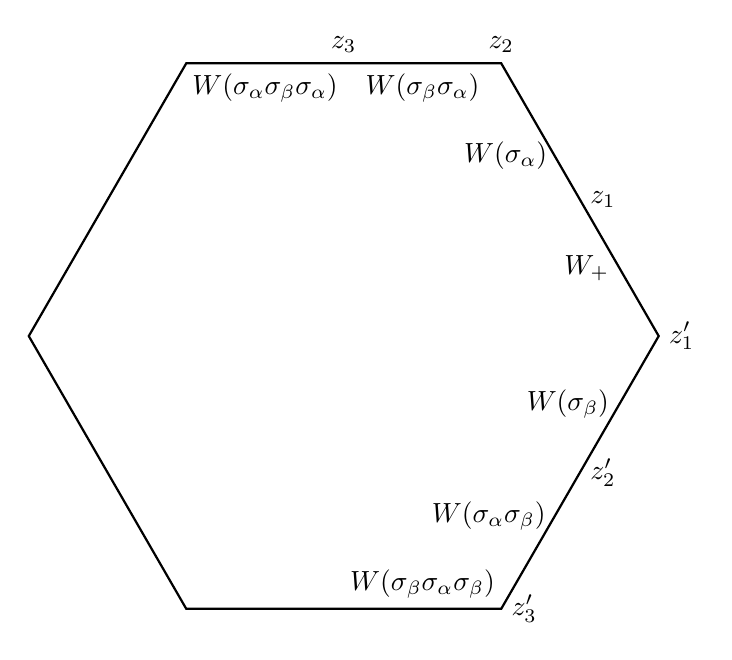
\begin{tikzpicture}[>=angle 90,scale=4]
\draw[thick]
(0,0) 
-- ++(0:0.5)
-- node[above]{$W(\sigma_\beta\sigma_\alpha\sigma_\beta)$} ++(0:0.5) node[below,right]{$z_3'$} 
-- node[left,above]{$W(\sigma_\alpha\sigma_\beta)$\phantom{XXXXX}} ++(60:0.5) node[below,right]{$z_2'$} 
-- node[above,left]{$W(\sigma_\beta)$} ++(60:0.5) node[right]{$z_1'$} 
-- node[below,left]{$W_+$} ++(120:0.5) node[above,right]{$z_1$}
-- node[left,below]{$W(\sigma_\alpha)$\phantom{XXXl}} ++(120:0.5) node[above]{$z_2$}
-- node[below]{$W(\sigma_\beta\sigma_\alpha)$} ++(180:0.5) node[above]{$z_3$}
-- node[below]{$W(\sigma_\alpha\sigma_\beta\sigma_\alpha)$} ++(180:0.5) 
-- ++(240:1) --cycle;
\end{tikzpicture}
\hrule
\vskip .15in
\medskip
\end{figure}
%\box \boxD




\noindent
Write
$$
\aligned
n_{w_1} &= \exp(z_{1}X_{-{\alpha}}), \\
n_{w_2} &= \exp(z_{2}X_{-{\beta}})\exp(z_{1}X_{-{\alpha}}), \\
n_{w_3 }&= \exp(z_{3}X_{-{\alpha}})\exp(z_{2}X_{-{\beta}})\exp(z_{1}X_{-{\alpha}}) .
\endaligned
$$
We now apply lemma 6.1 three times.  The {\it  first}  application gives
$$
{\alpha}(t_{2})z_{3}(y_{3}-u_{3}m_{{\delta}})+1 = 0
$$
where
$$
v_{2} = \exp(y_{3}X_{{\alpha}})^{{\alpha}}v_{2}\ {\text{and}}\ {\omega}_{2}
X_{{\delta}}{\omega}_{2}^{-1}=u_{3}X_{{\alpha}}.
$$
The {\it second}  application gives
$$
{\beta}(t_{1})z_{2}(y_{2}-u_{2}m_{{\epsilon}})+1 = 0
$$
where
$$v_{1} = \exp(y_{2}X_{{\beta}})^{{\beta}}v_{1}\ {\text{and}}\
{\omega}_{1}X_{{\epsilon}}{\omega}_{1}^{-1}=u_{2}X_{{\beta}};
$$
$$
t_{2} = t_{1}(-{\beta}(t_{1})z_{2})^{-{\beta}^{v}} ,
$$
$$
v_{2} = \exp({\beta}(t_{1})z_{2}X_{{\beta}}){\sigma}_{{\beta}}\exp(u_{2}
m_{{\epsilon}}X_{{\beta}})^{{\beta}}v_{1}\exp(-u_{2}m_{{\epsilon}}
X_{{\beta}}){\sigma}_{{\beta}}^{-1}.
$$
The {\it third}  application gives
$$
z_{1}(y_{1}-u_{1}m_{{\alpha}}) + 1 = 0
$$
where
$$y_{1} = 0\ {\text{and}}\  u_{1} = 1
$$
$$
\aligned
t_{1} &= (-z_{1})^{-{\alpha}^{v}} , \\
v_{1} &= \exp(z_{1}X_{{\alpha}}).
\endaligned
$$
Straightforward calculations give ${\beta}(t_{1}) = {\beta}(-z_{1}^{-\alpha^v})
= -z_{1}^{3}$, $${\alpha}(t_{2}) =
{\alpha}(t_{1})(-{\beta}(t_{1})z_{2})^{-<\alpha,\beta^v>}
= z_{1}z_{2},$$
$y_{1}=0$, $v_{1} = \exp(y_{2}X_{{\beta}})^{{\beta}}v_{1}$
$= \exp(z_{1}X_{{\alpha}})$, $y_{2} = 0$, $\exp(z_{1}X_{{\alpha}}) =$
${}^\beta v_1$.

\noindent
$$
\aligned
v_{2} =& \exp(y_{3}X_{{\alpha}})^{{\alpha}}v_{2} = {\epsilon}_{{\beta}}(*)
{\sigma}_{{\beta}}{\epsilon}_{{\alpha}}(z_{1}){\epsilon}_{{\gamma}}
(az_{1}u_{2}m_{{\epsilon}}){\epsilon}_{{\delta}}(*){\epsilon}_{{\zeta}}(*)
{\sigma}_{{\beta}}^{-1}
\\ =& {\epsilon}_{{\alpha}}(az_{1}u_{2}m_{{\epsilon}}
u_{2}')^{{\alpha}}v_{2}
. \endaligned$$
So $y_{3} = az_{1}u_{2}u_{2}'m_{{\epsilon}}$ where Ad ${\sigma}_{{\beta}}
(X_{{\gamma}})=u_{2}'X_{{\alpha}}$.
 So

$$z_{1}z_{2}z_{3}(au_{2}u_{2}'m_{{\epsilon}}z_{1}-u_{3}m_{{\delta}})+1 = 0$$
$$
-z_{1}^{3}z_{2}(-u_{2}m_{{\epsilon}})+1 = 0
$$
$$
-z_{1}(-u_{1}m_{{\alpha}})+1 = 0
$$
Thus $u_{1}m_{{\alpha}}=1/z_{1}, u_{2}m_{{\epsilon}}=-1/(z_{1}^{3}z_{2}),
u_{3}m_{{\delta}}=1/(z_{1}z_{2}z_{3}) + (au_{2}u_{2}'m_{{\epsilon}}z_{1})
= 1/(z_{1}z_{2}z_{3}) - au_{2}'/(z_{1}^{2}z_{2})$.

Now write $t_{3}'v_{3}'{\omega}_{3}'m_{3}' = n_{w_3'}$;
$t_{2}'v_{2}'{\omega}_{2}'m_{2}' = n_{w_2'};
t_{1}'v_{1}'{\omega}_{1}'m_{1}' = n_{w_1'}$.
 Write $n_{w_1'} = \exp(z_{1}'X_{-{\beta}}), \
n_{w_2'} = \exp(z_{2}'X_{-{\alpha}})
\exp(z_{1}'X_{-{\beta}})$, $$n_{w_3'} =
\exp(z_{3}'X_{-{\beta}})\exp(z_{2}'X_{-{\alpha}})\exp(z_{1}'X_{-{\beta}}).$$
 We now apply lemma 6.1 three more times.
 The {\it first}  application gives
$$
{\beta}(t_{2}')z_{3}'(y_{3}'-u_{3}'m_{{\zeta}})+1 = 0
$$
where $v_{2}' = \exp(y_{3}'X_{{\beta}})^{{\beta}}v_{2}'$ and
${\omega}_{2}'X_{{\zeta}}{\omega}_{2}^{\prime-1}=u_{3}'X_{{\beta}}$.
 The {\it second}  application gives
$$
{\alpha}(t_{1}')z_{2}'(y_{2}'-u_{2}'m_{{\gamma}})+1 = 0
$$
where
$$
v_{1}' = \exp(y_{2}'X_{{\alpha}})^{{\alpha}}v_{1}'\ {\text{and}}\
{\omega}_{1}'X_{{\gamma}}{\omega}_{1}^{\prime-1}=u_{2}'X_{{\alpha}};
$$
$$
t_{2}' = t_{1}'(-{\alpha}(t_{1}')z_{2}')^{-\alpha^v} ,
$$
$$
v_{2}' = \exp({\alpha}(t_{1}')z_{2}'X_{{\alpha}}){\sigma}_{{\alpha}}
\exp(u_{2}'m_{{\gamma}}X_{{\alpha}})^{{\alpha}}v_{1}'
\exp(-u_{2}'m_{{\gamma}}X_{{\alpha}}){\sigma}_{{\alpha}}^{-1}.
$$
The {\it third}  application gives
$$
z_{1}'(y_{1}'-u_{1}'m_{{\beta}})+1 = 0\ {\text{where}}\
y_{1}' = 0\  {\text{and}}\ u_{1}' = 1,
$$
$$
\aligned
t_{1}' &= (-z_1')^{-\beta^v} ,\\
v_{1}' &= \exp(z_{1}'X_{{\beta}}) .
\endaligned
$$
Now we have as a consequence ${\alpha}(t_{1}') =
{\alpha}(-z_{1}^{\prime-\beta^v}) = -z_{1}'$,
$$
\beta(t_{2}') = {\beta}(t_{1}')(-{\alpha}(t_{1}')z_{2}')^{-<\beta,\alpha^v>}
= z_{1}'z_{2}^{\prime3},
$$
$$
y_{1}'= 0,
$$
$$
v_{1}' = \exp(y_{2}'X_{{\alpha}})^{{\alpha}}v_{1}' = \exp(z_{1}'X_{{\beta}}),
$$
$$
y_{2}' = 0, {}^\alpha v_{1}' = \exp(z_{1}'X_{{\beta}}).
$$
$$
v_{2}' = \exp(y_{3}'X_{{\beta}})^{{\beta}}v_{2}' = {\epsilon}_{{\alpha}}(*)
{\sigma}_{{\alpha}}{\epsilon}_{{\alpha}}(u_{2}'m_{{\gamma}})
{\epsilon}_{{\beta}}(z_{1}'){\epsilon}_{{\alpha}}
(-u_{2}'m_{{\gamma}}){\sigma}_{{\alpha}}^{-1} =
$$
%
$$
\e_{{\alpha}}(*){\sigma}_{\alpha}\e_\beta(z_{1}')
{\e}_\gamma(*)\e_\delta(*)\e_\e(c(-u_{2}'m_{{\gamma}})^{3}z_{1}')
\e_\zeta(*) {\sigma}_{\alpha^{-1}} =
$$
$$
{\epsilon}_{{\beta}}(c(-u_{2}'m_{{\gamma}})^{3}z_{1}'u_{2})^{{\beta}}v_{2}'.
$$
So
$$
y_{3}' = -c(u_{2}'m_{{\gamma}})^{3}z_{1}'u_{2}
$$
where
$$
{\text{Ad}}\ {\sigma}_{{\alpha}}(X_{{\epsilon}}) = u_{2}X_{{\beta}}.
$$
This gives the equations
$$
-z_{1}'u_{1}'m_{{\beta}}+1=0\ {\text{or}}\ u_{1}'m_{{\beta}} = 1/z_{1}'
$$
$$
z_{1}'z_{2}'u_{2}'m_{{\gamma}}+1 = 0\ {\text{or}}\ u_{2}'m_{{\gamma}} =
-1/(z_{1}'z_{2}')
$$
$$
z_{1}'z_{2}^{\prime3}z_{3}'(-cu_{2}^{\prime3}m_{{\gamma}}^{3}z_{1}'u_{2} -
u_{3}'m_{{\zeta}})+1 = 0
$$
$$
\hbox{or}\quad  u_{3}'m_{{\zeta}} = 1/(z_{1}'z_{2}^{\prime3}z_{3}') -
c(u_{2}'m_{{\gamma}})^{3}z_{1}'u_{2} =
$$
$$
= 1/(z_{1}'z_{2}^{\prime3}z_{3}') + cu_{2}/(z_{1}^{\prime2}z_{2}^{\prime3}) .
$$
Humphreys \cite{MR0396773} shows that Ad ${\sigma}_{{\alpha}}(X_{{\delta}}) =
-X_{{\gamma}}$, Ad ${\sigma}_{{\alpha}}(X_{{\epsilon}}) =
X_{{\beta}}$, Ad ${\sigma}_{{\alpha}}(X_{{\zeta}}) =
X_{{\zeta}}$, Ad ${\sigma}_{{\beta}}(X_{{\gamma}}) =
-X_{{\alpha}}$, Ad ${\sigma}_{{\beta}}(X_{{\delta}}) =
X_{{\delta}}$, Ad ${\sigma}_{{\beta}}(X_{{\zeta}}) = -X_{{\epsilon}}$.
 From this it follows that $u_{1}=1, u_{2}=1, u_{3} = 1, u_{1}' =
1, u_{2}'=-1, u_{3}' = -1$.
 Substituting these values into the expressions for $m_{-}$, we obtain the
result.
\end{proof}


\section{The\ Functions\ $n_\gamma$}

   The functions $n_{{\gamma}}$ are much easier to compute for the classical
groups.
 In fact lemma 6.1 is not needed.
To illustrate we calculate them for $SL(n)$.
 (The same method gives all classical groups).

\begin{lemma}{Lemma 8.1}
$$
n_{\alpha_r+\ldots +\alpha_{r+s}}  =
1/(z(W_{0},{\alpha}_{r})z(W_{1},{\alpha}_{r+1})\ldots z(W_{s},{\alpha}_{r+s}))
$$
where $W_{0} = W_{+}$, and $W_{t+1}$ is adjacent to $W_{t}$ through a wall of
type ${\alpha}_{r+t} (t = 0,\ldots ,s-1)$.
\end{lemma}

\begin{proof}    Represent $SL(n)$ in the standard way with ${\BB} =
B_{0}$ upper triangular and $B_{{\infty}}$ lower triangular.
 The relation ${\BB}^{\omega n}  =
{\BB}^{n_w}$  is equivalent to ${\omega}nn_{w}^{-1}
\in {\BB}$.
 Let ${\sigma}_{i} = {\sigma}_{\alpha_{r+i}},
X_{i} = X_{-{\alpha}_{r+i}}, z_{i} = z(W_{i},{\alpha}_{r+i}),
{\epsilon}_{i}(x) = \exp(xX_{i})$,\ $i=0,\ldots ,s$.
 Then $k_{t}\ {\mathrel{\mathop =^{(def)}}}\ {\omega}nn_{w}^{-1} =$
$$
{\sigma}_{t}\ldots {\sigma}_{0}n{\epsilon}_{0}(-z_{0})\ldots {\epsilon}_{t}(-z_{t})
\in B .
$$
Also
$$
k_{t+1} = {\sigma}_{t+1}{\sigma}_{t}\ldots {\sigma}_{0}n{\epsilon}_{0}(-z_{0})
\ldots {\epsilon}_{t}(-z_{t}){\epsilon}_{t+1}(-z_{t+1})
$$
$$
= {\sigma}_{t+1}k_{t}{\epsilon}_{t+1}(-z_{t+1}) \in B .
$$
Since ${\sigma}_{t+1}$ and ${\epsilon}_{t+1}(-z_{t+1})$ belong to the rank
one subgroup with Lie algebra $X_{{\alpha}}, X_{-{\alpha}}, H_{{\alpha}}$
where ${\alpha} = {\alpha}_{r+t+1}$  we can compute this last
product inside $SL(2)$ provided that we can determine the coefficients of
$k_{t}$ in the $c_{i,i}, c_{i,i+1}, c_{i+1,i}$ and $c_{i+1,i+1}$
positions where\ $i = r+t+1$.	 Since $k_{t} \in B$,
$c_{i+1,i} = 0$.
 ${\sigma}_{i}$ acts as the permutation $(r+i,r+i+1)$ on the rows of
$nn_{w}^{-1}$.
 So ${\sigma}_{t}\ldots {\sigma}_{0}$ acts as the permutation
$(r+t,r+t+1)\ldots (r,r+1) = (r+t+1,r+t,\ldots ,r)$ on the rows of $nn_{w}^{-1}$.
 Thus the $r+t+1st$ row of ${\omega}nn_{w}^{-1}$ equals the $r$th row of
$nn_{w}^{-1}$ and the $r+t+2nd$ row of ${\omega}nn_{w}^{-1}$ equals the
$r+t+2nd$ row of $nn_{w}^{-1}$.
 Since $n_{w}^{-1} = {\epsilon}_{0}(-z_{0})\ldots {\epsilon}_{t}(-z_{t})$ the
$i$th and $i+1$st columns of $nn_{w}^{-1}$ are the same as the respective
columns of $n$.
 Thus $c_{i+1,i+1} = 1$, $c_{i,i+1} = n_{r,r+t+2}  =
n_{\alpha_r+\ldots +\alpha_{r+t+1}}$, $c_{i,i} = n_{r,r+t+1}$ $ =
n_{\alpha_r+\ldots + \alpha_{r+t}}.$

   We have the matrix product in SL(2)
$$
{\begin{pmatrix} \prelax
%\format \r &\quad \c \\
 0 & 1 \\ -1 & 0 \end{pmatrix}}\
{\begin{pmatrix} \prelax  x & y \\ 0 & 1 \end{pmatrix}}\ {\begin{pmatrix} \prelax
%\format  \r &\quad \c \\
1 & 0 \\ -z & 1 \end{pmatrix}}\ =\
{\begin{pmatrix} \prelax
%\format \c &\quad \r \\
 -z & 1 \\ yz-x & -y \end{pmatrix}}\
\in B .
$$
The equality $x = yz$ becomes $c_{i,i} = z_{t+1}c_{i,i+1}$.
$$
n_{\alpha_r+\ldots +\alpha_{r+t}}/z(W_{t+1},
{\alpha}_{r+t+1}) = n_{\alpha_r+\ldots +\alpha_{r+t+1}},
$$
so by induction
$$
n_{\alpha_r+\ldots +\alpha_{r+s}}  =
1/(z(W_{0},{\alpha}_{r})z(W_{1},{\alpha}_{r+1})\ldots z(W_{s},{\alpha}_{r+s})).
$$
\end{proof}
{\medskip}

Also by a similar argument the following lemma is proved.

\medskip

\begin{lemma}{Lemma\ 8.2}  Let $m_{{\beta}}$ be the ${\beta}$th coefficient of
the inverse of $n$, let $W_{0}=W_{+}$ and let $W_{j+1}$ be the Weyl chamber
adjacent to $W_{j}$ through the wall $(W_{j},{\alpha}_{r-j})$ then
$$
m_{\alpha_{r-s}+\ldots +\alpha_{r}} = (-1)^{s+1}/z(W_{0},
{\alpha}_{r})z(W_{1},{\alpha}_{r-1})\ldots z(W_{s},{\alpha}_{r-s}) .
$$
\end{lemma}

\begin{proof}    Again represent $B_{0}$ in $SL(n)$ as the upper triangular
matrices and
$B_{{\infty}}$ as the lower triangular matrices.
 The calculation takes place entirely inside a Levi subgroup of $P_{{\Sigma}}$
where $P_{{\Sigma}}$ is the parabolic subgroup given by the simple roots
${\Sigma} = \{{\alpha}_{r-s},\ldots ,{\alpha}_r\}$.  Thus we reduce immediately
to the case where $r-s = 1$ and $r = n-1$.
 Let ${\sigma}_{i} = {\sigma}_{\alpha_i}, X_{i} =
X_{-\alpha_i},$ and let $z_{i} = z(W_{i-1},{\alpha}_{n-i})$.
 As in the previous lemma we have ${\omega}nn_{w}^{-1} \in B_{0}$.

Let
$$
n_{w} = \exp(z_{n-1}X_{1})\ldots \exp(z_{1}X_{n-1}).
$$
Then
$$
{\sigma}_{1}\ldots {\sigma}_{n-1}n\exp(-z_{1}X_{n-1})\ldots \exp(-z_{n-1}X_{1})
\in B .
$$
To make it possible to use the previous lemma we apply the involution $g {\to}
J^{t}g^{-1}J$ to the group $SL(n)$ where
$$
J =
\begin{pmatrix} \prelax  0 & 0 & 0 & 0 & 1 \\
0 & 0 & 0 & 1 & 0 \\
0 & 0 & \ldots & 0 & 0 \\
0 & 1 & 0 & 0 & 0 \\
1 & 0 & 0 & 0 & 0 \end{pmatrix} .
$$
Under this involution $X_{i} {\to} -X_{n-i}, {\sigma}_{i} {\to}
{\sigma}_{n-i}^{-1}, n {\to} J^{t}n^{-1}J$.
 Thus ${\omega}nn_{w}^{-1}$ is sent to
$$
\sigma_{n-1}^{-1}\ldots {\sigma}_{1}^{-1}J^{t}n^{-1}J\exp(z_{1}X_{1})\ldots
\exp(z_{n-1}X \in B .
$$
Now the coefficient in the $(1,n)$th position of $J^{t}n^{-1}J$ equals
$m_{\alpha_1+\ldots +\alpha_{n-1}}$.  We now apply the
previous lemma bearing in mind that the signs of the $z_{i}$ have been
reversed.
 This gives the result.
\end{proof}

\section{The\  Fundamental\  Divisors\  on\ $Y_\Gamma$}

   There is a morphism from each divisor $E$ in $Y_{{\Gamma}}$ to the variety
${\xi}^{-1}(1)$ in $Y_{1}$.
 An irreducible divisor $E$ in $Y_{{\Gamma}}$ whose image in $Y_{1}$ lies in the
complement of $Y^{\prime\prime}$ is called a {\it spurious\ divisor}.  If there are walls
$(W,{\alpha})$ and $(W',{\alpha})$ such that $z(W,{\alpha})/z(W',{\alpha})
(= z_{1}(W,{\alpha})/z_{1}(W',{\alpha})) = 0$ on $E$, then $E$ is a spurious divisor.
 By \cite{MR701566}*{\S3.8} the condition that $z(W,{\alpha})/z(W',{\alpha}) = 0$ is
independent of the coordinate patch.
 All other irreducible divisors on $Y_{{\Gamma}}$ are called {\it  fundamental divisors}.
An open dense set of a fundamental divisor lies over $Y''$.

   Every fundamental divisor in $Y_{{\Gamma}}$ maps to (but not necessarily onto)
an irreducible component of ${\xi}^{-1}(1)$ in $Y_{1}$.
 Much can be learned about the fundamental divisors by studying their image in $Y_{1}$.
 In fact nearly all calculations with fundamental divisors can be reduced to
calculations in the singular variety $Y_{1}$.
 We use the coordinates developed in this chapter to study the fundamental divisors.


   Weil divisors are defined on any variety which is regular in codimension
one \cite{MR0463157}.
 I have not proved in general that $Y_{1}''$ is regular in codimension one,
although it seems likely that it is.
 Thus whenever I speak of a divisor $E$ on (a subvariety of) $Y''$, I must first
produce an appropriate subvariety of $Y''$ which is regular in codimension one.
 Assuming that this can be done, we also call the divisors of ${\lambda} = 0$
in $Y''_{1}$ fundamental divisors.
 Provided appropriate regularity conditions hold, they are given by the
irreducible components of the set of the following set of equations with
${\lambda}$ set equal to $0$:
$$
w({\gamma}){\lambda} = x({\gamma}) \prod
z({\alpha})^{m({\alpha})} : {\gamma} = \sum m({\alpha}){\alpha}
$$
$$
w({\gamma})x({\beta}) = w({\beta})x({\gamma}) \prod
z({\alpha})^{m({\alpha})}  : {\gamma}-{\beta} = \sum m({\alpha}){\alpha}
$$
(The full list of equations here includes all equations holding on the Zariski
closure of the variety defined for ${\lambda}\ne 0$ by ${\lambda}w({\gamma})$
$= x({\gamma})\prod z({\alpha})^{m({\alpha})} : {\gamma} =
\sum m({\alpha}){\alpha}.)$

   Recall that $w({\alpha})=1$ for ${\alpha}$ simple.
 There are $2N+1$ variables in the set
 $$
 \{{\lambda},w({\gamma}),x({\gamma}),
z(\alpha)\}\backslash \{w(\alpha) : {\alpha} \hbox{ simple}\}
$$
\ where  $N =
(dim(G)-rank(G))/2 = dim(S''(B_{{\infty}},B_{0}))$.
 For any positive root ${\gamma}$, set
 $${\gamma}=\sum m_{{\gamma}}
({\alpha}){\alpha}, \quad m_{{\gamma}}=\sum m_{{\gamma}}({\alpha})
\quad\hbox{and }\quad
z({\gamma}) = \prod z({\alpha})^{m_\gamma(\alpha)}.$$
For every set
${\Sigma}$ of simple roots, we describe a divisor $E_{{\Sigma}}$ (again
assuming appropriate regularity).
 Let ${\Sigma}'$ be the positive roots spanned by ${\Sigma}$; and let
${\Sigma}^{c}$ be the other positive roots.
 $E_{{\Sigma}}$ is the closure in $Y^{\prime\prime}$ of the subvariety defined by

\begin{enumerate}[label=\roman*)]
\item ${\lambda}=0$
\item $x({\alpha})\ne 0$ for ${\alpha} \notin  {\Sigma} : {\alpha}$
simple
\item $z({\alpha})\ne 0$ for ${\alpha} \in {\Sigma} : {\alpha}$ simple.
\end{enumerate}



\begin{proposition}{Proposition 9.1}   Let $Y''_{{\Sigma}}$ be the open subvariety of $Y''$
consisting of points on $Y''$ which satisfy conditions $(ii)$ and $(iii)$.
 The open subvariety of $Y''$ consisting of the union of $Y''_{{\Sigma}} {\
\forall\ } {\Sigma}$ is regular in codimension one.
 $E_{{\Sigma}}$ is an $O_{{\Sigma}}$-divisor where $O_{{\Sigma}}$ is the
Richardson class of the parabolic subgroup $P_{{\Sigma}}$.
 The Igusa constant $a(E_{{\Sigma}})$ is one.
 The Igusa constant ${\beta}(E_{{\Sigma}})-1$ equals $(dim(C_{G}(u)-rank(G))/2$.
\end{proposition}

\begin{proof}    The local ring near a generic point of $E_{{\Sigma}}$ is
regular because it is generated by $\{{\lambda},x({\gamma}):{\gamma} \in
{\Sigma}^{c}, w({\gamma}):{\gamma} \in {\Sigma}', z({\alpha}):{\alpha} \in
{\Sigma\} }$  for :
$$
z({\alpha}) = {\lambda}/x({\alpha}) : {\alpha} \notin {\Sigma};
$$
$$
x({\gamma}) = {\lambda}w({\gamma})/z({\gamma}) : {\gamma} \in {\Sigma}';
$$
$$
w({\gamma}) = x({\gamma})\prod z(\alpha)^{m({\alpha})}/x({\alpha}_{0}) : {\gamma} \in {\Sigma}^{c},
{\alpha}_{0} \notin
{\Sigma}, {\gamma}-{\alpha}_{0}=\sum m({\alpha}){\alpha}
$$
$(\gamma$ not simple).
 We see that $x({\gamma})=0$ on $E_{{\Sigma}}$ if and only if ${\gamma} \in
{\Sigma}'$.
 This proves that the subvariety of $Y''$ of the lemma is regular in codimension
one.
 This also shows that that $E_{{\Sigma}}$ is an $O_{{\Sigma}}$-divisor where
$O_{{\Sigma}}$ is the Richardson class of the parabolic $P_{{\Sigma}}$.
 We also see that the Igusa constant $a(E_{{\Sigma}})$, which is defined to
be the multiplicity with which ${\lambda}$ vanishes along $E$, equals one.

   Spaltenstein \cite{MR672610}*{\S3.2} tells us that $\dim C_{G}(v) = \dim(M_{{\Sigma}})$
where $M_{{\Sigma}}$ is a Levi component associated to the parabolic
$P_{{\Sigma}}$ and $v \in O_{{\Sigma}}$.
 The form on $X^{0}$ is given by
$$
{\omega}_{X} = d{\lambda}\wedge
dx({\alpha})\wedge dx({\beta})\wedge \ldots \wedge d{\nu}_{{\alpha}}
\wedge d{\nu}_{{\beta}}\wedge \ldots
$$
To pass to the form in a neighborhood of $E_{{\Sigma}}$ we make the
substitution $x({\gamma}) = {\lambda}w({\gamma})/z({\gamma})$ for ${\gamma}
\in {\Sigma}'$ where $z({\gamma})$ is defined to be the product
$\prod z({\alpha})^{m({\alpha})}$.
 We can pull the factors ${\lambda}$ out of the form to obtain
$$
\omega_{X} = {\lambda}^{\vert {\Sigma}'\vert} d{\lambda}\wedge \prod
d(w({\gamma})/z({\gamma}))\wedge \prod dx({\beta})\ldots
= {\lambda}^{\beta(E)-1}d{\lambda}\wedge\ldots .
$$
The constant $b(E)-1$ is defined to be the multiplicity of the zero of
${\omega}_{X}$ along $E$ which in this case is $\vert {\Sigma}'\vert .$
When $a(E)=1, {\beta}(E) = b(E)$.
 But then $2({\beta}(E)-1) = 2\vert {\Sigma}'\vert  =
dim(M_{{\Sigma}})-rank(G)$.
 This completes the proof.
\end{proof}
{\medskip}



   The result that ${\beta}(E)-1 = (dim(C_{G}(u))-rank(G))/2$ is to be expected.
 Harish-Chandra has proved the following result in characteristic zero.

\begin{proposition}{Proposition 9.2}   Let $O$ be an $F$-unipotent conjugacy class.
 Let ${\Gamma}({\gamma})$ be
the $O$-germ of an orbital integral relative to the measure
$$
\prod (1-{\alpha}^{-1}({\gamma})){\omega}_{T\backslash G}.
$$
Let $r = dim(C_{G}(u))-rank(G)$.
 Let $X$ be a vector in the Lie algebra of $T$ which does not lie in any
singular hyperplane.
 Then ${\Gamma}(\exp({\lambda}^{2}X)) =
\vert {\lambda}\vert ^{r}{\Gamma}(\exp(X))$.
\end{proposition}

\begin{proof}    \cite{MR0579175}
\end{proof}

{\medskip}

   Let $E_{1}$ denote a globally defined divisor which is equal to
$E_{{\Sigma}}$ on the given coordinate patch $Y^{\prime\prime}(B_{{\infty}},B_{0})$.
 The following lemma insures that ${\Sigma}$ is independent of the
coordinate patch and that divisors which are distinct on one coordinate patch
are distinct on every coordinate patch.

\begin{lemma}{Lemma 9.3}    Let $(u,B(W))$ be a generic point of $E_{1}$.
 Let $P_{{\Sigma}'}$ be a parabolic subgroup minimal among those parabolic
subgroups containing $B(W)$ for all $W$.
 Then ${\Sigma} = {\Sigma}'$.
\end{lemma}

\begin{proof}    On a coordinate patch $Y''(B_{{\infty}},B_0)$, we have seen
that $u$ is a Richardson class of the parabolic subgroup $P_{{\Sigma}}$.
 Also $z({\alpha}) = 0, {\alpha} \notin {\Sigma}$.
 This implies that $B(W) \in P_{{\Sigma}}$ for all $W$.
 $E_{1}$ is the closure of $E_{{\Sigma}}$, so that $B(W) \in P_{{\Sigma}}$
for all $W$ and all points in $E_{1}$.
 Since $z(W_{+},{\alpha})\ne 0$ for ${\alpha} \in {\Sigma}$ at the generic
point, we have $B(W_{+})\ne B(W({\sigma}_{{\alpha}}))$, so that ${\alpha}
\in {\Sigma}'$ for any $P_{{\Sigma}'}$ containing $B(W)$ for all $W$.
 Thus ${\Sigma} {\subseteq} {\Sigma}'$, and $P_{{\Sigma}}$ is minimal.
\end{proof}

{\medskip}

   The following simple fact will be needed in the proof of proposition
9.5.
 We continue to work over the algebraic closure $\Fb$  of $F$.

\begin{lemma}{Lemma 9.4}  Every irreducible component of ${\lambda} = 0$ has
codimension one in $Y''$.
\end{lemma}

\begin{proof}    This follows directly from \cite{MR971985}*{p.65}
\end{proof}

{\medskip}

   The following proposition will not be needed in what follows.

\begin{proposition}{Proposition 9.5}   When $G = A_{n}$, the variety $Y''$ is regular in
codimension one.
 The only divisors on $Y''$ for a group of type $A_{n}$ are $E_{{\Sigma}}
{\ \forall\ } {\Sigma}$.
\end{proposition}


\begin{proof}   If we show that every point of ${\lambda} = 0$ lies inside
one of the divisors $E_{{\Sigma}}$, then the result follows from proposition 9.1.
 Let $E$ be a component of ${\lambda} = 0$.
 We will use the following observation repeatedly.
 If $E$ has dimension $x$ and the coordinate ring of $E$ is generated by $x+r$
functions then at most $r$ of those functions equal zero.

Let $R$ be the set of roots ${\gamma}$ such that $x({\gamma})\ne 0$ on $E$.
 Let $R_{\min}$ be the subset of $R$ such that if ${\gamma} \in R_{\min}$ and
${\gamma}-{\beta}=\sum m({\alpha}){\alpha}$ with $m({\alpha}) \ge 0$ then
$x({\beta}) = 0$.
 Since $w({\alpha}) = 1$ for ${\alpha}$ simple, the functions $\{w(\gamma)\}$
are indexed by ${\gamma} \in {\Phi}^{+}\backslash {\Delta}$ where
${\Phi}^{+}$ are the positive roots and ${\Delta}$ are the simple roots.
 Then there are $\vert \{\lambda\}\vert  + \vert \{w(\gamma)\}\vert  +
\vert \{z(\alpha)\}\vert + \vert \{x(\gamma)\}\vert  + \vert
\{$ coefficients of ${\nu}\}\vert  = 1 + (N-{\ell}) + {\ell} + N + N = 3N + 1$
variables where ${\ell} = rank(G)$ and $2N = (dim(G)-{\ell})$.
 Also by (9.4) the dimension of $E$ equals $2N$.
 The observation above tells us that the number of variables we eliminate
plus the number that are identically zero is at most $N+1$.

   We know by definition of $R$ that $x({\beta}) = 0$ on $E$ for ${\beta} \in
{\Phi}^{+}\backslash R$.
 If ${\gamma} \in R\backslash R_{\min}$ then there exists a positive root
${\beta}$ with $x({\beta})\ne 0$ such that ${\gamma}-{\beta} =
\sum m({\alpha}){\alpha}$, $m({\alpha}) \ge 0$.
 For such ${\gamma}$ the variable $w({\gamma})$ can be eliminated through the
equation $$w({\gamma})x({\beta}) = x({\gamma})w({\beta}) \prod
z({\alpha})^{m({\alpha})}.$$
 We know that that ${\lambda} = 0$ on $E$.
 If ${\alpha} \in R_{\min} {\cap} {\Delta}$ then the equation
$z({\alpha})x({\alpha}) = {\lambda}$ allows one to eliminate $z({\alpha})$.
In summary if ${\delta} = \vert R_{\min}\backslash {\Delta}\vert$  then we
either eliminate or set to zero $(N-\vert R\vert ) + \vert R\backslash
R_{\min}\vert  + 1 + \vert R_{\min} {\cap} {\Delta}\vert  =
N + 1 - {\delta}$ variables.

   Now specialize to the case $G = A_{n}$.
 We can write the elements of $R_{\min}$ as ${\gamma}_1,
\ldots ,{\gamma}_p$  where ${\gamma}_i
= {\alpha}_{r_{i}} +\cdots + {\alpha}_{r_{i}+s_{i}}$  with $r_{1} < \cdots <
r_{p}$ and $r_{1}+s_{1}< \cdots < r_{p}+s_{p}$ and $s_{i} \ge 0$.
\end{proof}

\begin{lemma}{Lemma  9.6}   $R_{\min} {\subseteq} {\Delta}$.
\end{lemma}

\begin{proof}    For each ${\gamma} \in R_{\min}\backslash {\Delta}$,
write $w({\gamma})x({\beta})=w({\beta})x({\gamma})z({\alpha}_{r})$ where
${\gamma} = {\alpha}_{r} + \ldots + {\alpha}_{r+s}$ and ${\beta} =
{\gamma}-{\alpha}_{r}$.
 By the definition of $R_{\min}, x({\beta}) = 0$ and $x({\gamma}) \ne 0$.
 So $w({\beta})z({\alpha}_{r}) = 0$.
 From the the inequalities $r_{1} < \cdots < r_{p}$ it follows that the
variables $z({\alpha}_{r})$ are distinct and do not equal any of the variables
$z({\alpha}) ({\alpha} \in R_{\min} {\cap} {\Delta})$ eliminated in the
previous paragraph.
 From the same inequalities it follows that the variables $w({\beta})$ are
distinct.
 Furthermore ${\beta}$ cannot lie in $R\backslash R_{\min}$ for this would
force ${\gamma}$ to lie in $R\backslash R_{\min}$ as well.
 Thus the equations $w({\gamma}-{\alpha}_{r})z({\alpha}_{r}) =
0 {\ \forall\ } {\gamma} \in R_{\min}\backslash {\Delta}$ force
${\delta} = \vert R_{\min}\backslash {\Delta}\vert$  addition variables to zero.
 We have now eliminated or set to zero $N+1$ distinct variables.
 No further variables can be eliminated or set to zero without contradiction.

   Set $w_{i} = w({\alpha}_{r_{i}} + \cdots +{\alpha}_{r_{i}+s_{i}-1})$ and
$z_{i} = z({\alpha}_{r_{i}+s_{i}})$ for $i \in \{1,\ldots ,p\}. $
Let $q$ be the largest element of $\{1,\ldots ,p\}$ such that
${\gamma}_{q} \in R_{\min}\backslash {\Delta}$.
 As above we have $w_{i}z_{i} = 0$.
 Suppose $z_{q} = 0$, then we must have $z_{q} = z({\alpha}_{r})$ for some $r$.
 But since $r_{q-1} < r_{q} < r_{q}+s_{q} < r_{q+1}+s_{q+1} = r_{q+1}$, this
is impossible.  Thus $z_{q} \ne 0$ and $w_{q}=0$.
 Continuing inductively suppose that $z_{j+1},\ldots ,z_{q} \ne  0$ and
${\gamma}_{j},\ldots ,{\gamma}_{q} \in R_{\min}\backslash {\Delta}$.
 Then it follows that again $z_{j} \ne 0$ and $w_{j} = 0$.
 If $j$ is now chosen to be the smallest integer such that
${\gamma}_{j},\ldots ,{\gamma}_{q} \in R_{\min}\backslash {\Delta}$ then
$w_{j}=0 .$  Since ${\gamma}_{j-1} \in {\Delta}, w_{j}$ cannot equal any
of the variables previously set to zero.
 This gives a contradiction.  Thus $R_{\min} {\subseteq} {\Delta}$.

   Since no variables equal zero on $E$ other than those already specified,
we have on $E \ \ (i) \ {\lambda}=0, \ \ (ii) \ x({\alpha})\ne 0$ for ${\alpha} \notin
{\Delta}\backslash R_{\min}$ (that is ${\alpha} \in R_{\min}),
\ \ (iii) \ z({\alpha})\ne 0$ for ${\alpha} \in {\Delta}\backslash R_{\min}$.
 These are the conditions holding on an open set of the divisor $E_{{\Sigma}}$
with ${\Sigma} = {\Delta}\backslash R_{\min}$.
\end{proof}
%% end of bthis.tex

%% start of cthis.tex

%
\chapter{Groups of Rank Two}
%


\section{Zero\ Patterns}



  Consider the variety of stars $S_{1}$ and a divisor $E$.
 For every coordinate patch $S_{1}(B_{{\infty}},B_{0})$ and simple root
${\alpha}$ select a chamber $W_{\alpha}$ such that
$z_{1}(W_{\alpha},{\alpha})\ne 0$ on $E$.
 Certain of the variables $z(W,{\alpha})/z(W_{\alpha},{\alpha})
(= z_{1}(W,{\alpha})/z_{1}(W_{\alpha},{\alpha}))$ will vanish identically
on $E$.
  This gives a {\it zero pattern}, i.e.,
a map ${\theta}_{1}$ from the walls to $\{0,1\}$, by
${\theta}_{1}(W,{\alpha}) = 0$ if and only if $z(W,{\alpha})/z(W_{\alpha},
{\alpha}) = 0$ on $E$.
 The zero pattern depends only on $E$ and not on the choices
$(B_{{\infty}},B_{0})$ and $W_{\alpha}$.
 The first part of this chapter studies the zero patterns for groups of
rank two.

   The rank two zero patterns will then be used to prove a result about
the divisors for an arbitrary group.
 Let ${\theta}_{1}$ be a zero pattern.
 For a fixed point $p$ (which is not necessarily a closed point of the
variety), a {\it special node}  is a node such that at least one wall of
each type is non-zero but that at least one wall is zero.
 By the nature of the equations at a node of type $A_{1} \times A_{1}$,
\begin{figure}[htb]
\centering
\begin{tikzpicture}[>=angle 90,scale=1.5]
\draw[thick]
(0,0) node[above]{$\phantom{-}y$} node[below]{$-y$}
-- ++(0:2) node[above]{$\phantom{-}y$} node[below]{$-y$}
(1,-1) node[left]{$x$} node[right]{$-x$}
-- ++(90:2) node[left]{$x$} node[right]{$-x$};
\end{tikzpicture}
%\hrule
\vskip .15in
\medskip
\end{figure}
%\medskip
%DIAGRAM5
%\sh{-20}{\box\boxE}
%\medskip

\noindent
a special node must be of type $A_{2}, B_{2}$, or $G_{2}$.
  The following proposition indicates the importance of special nodes.

\begin{proposition}{Proposition 1.1}   Let $G$ be a group of semi-simple rank $2$.
 Suppose that at a generic point of a divisor $E$ there is a special node.
 Then $E$ makes no contribution to the subregular germ.
 \end{proposition}

   The proof of this proposition is the subject of the second half of
this chapter.

   Fix a torus $T$ and a Borel $B$ of $G$ and let the positive roots be
$$
\begin{matrix}
%\format \l &\qquad \qquad \l \\
{\alpha}, {\beta}, {\g} = {\alpha}+{\beta}  &\ \  A_{2}\phantom{.} \\
{\alpha}, {\beta}, {\g} = {\alpha}+{\beta},\ {\delta} = 2{\alpha}+{\beta}
&\ \  B_{2}\phantom{.} \\
{\alpha}, {\beta}, {\g} = {\alpha}+{\beta}, {\delta} = 2{\alpha}+{\beta},
{\e} = 3{\alpha}+{\beta}, {\z} = 3{\alpha}+2{\beta} &\ \ G_{2}.
\end{matrix}
$$

We will take products according to this order on the roots.

\medskip

\begin{lemma}{Lemma 1.2}   $(G_{2})$

${\e}_{\alpha}(x_{1}){\e}_{\beta}(y_{1}){\e}_{\alpha}
(x_{2}){\e}_{\beta}(y_{2})\ldots
{\e}_{\alpha}(x_{n}){\e}_{\beta}(y_{n}) = $

${\e}_{\alpha}(a_{n}){\e}_{\beta}(b_{n}){\e}_{{\alpha} +
{\beta}}(c_{n}){\e}_{2{\alpha}+{\beta}}(d_{n}){\e}_{3{\alpha} +
{\beta}}(e_{n}){\e}_{3{\alpha}+2{\beta}}(f_{n})$

\noindent
where
$$
\aligned
a_{n} &= x_{1} + x_{2} +\ldots + x_{n} \\
b_{n} &= y_{1} + y_{2} +\ldots + y_{n} \\
c_{n} &= (x_{2}+\ldots +x_{n})y_{1} + (x_{3}+\ldots +x_{n})y_{2} + \ldots +
x_{n}y_{n-1}\\
d_{n} &= (x_{2}+\ldots +x_{n})^{2}y_{1} + (x_{3}+\ldots +x_{n})^{2}y_{2} +
\ldots + x_{n}^{2}y_{n-1}\\
e_{n} &= (x_{2}+\ldots +x_{n})^{3}y_{1} + (x_{3}+\ldots +x_{n})^{3}y_{2} +
\ldots + x_{n}^{3}y_{n-1}
\endaligned
$$
\end{lemma}

\begin{proof}    For $n = 1$ the statement is obvious.
 We proceed by induction.  By lemma II.7.1,

${\e}_{\alpha}(a_{n-1}){\e}_{\beta}(b_{n-1})
{\e}_{{\g}}(c_{n-1}){\e}_{{\delta}}(d_{n-1})
{\e}_{{\e}}(e_{n-1}){\e}_{{\z}}(f_{n-1})
{\e}_{\alpha}(x_{n}){\e}_{\beta}(y_{n})$

$= {\e}_{\alpha}(a_{n-1}+x_{n}){\e}_{\beta}(b_{n-1})
{\e}_{{\g}}(b_{n-1}x_{n}+c_{n-1}){\e}_{{\delta}}
(d_{n-1}+2x_{n}c_{n-1}+x_{n}^{2}b_{n-1})$

${\e}_{{\e}}(e_{n-1}+3x_{n}d_{n-1}+3x_{n}^{2}c_{n-1} +
x_{n}^{3}b_{n-1}){\e}_{{\z}}(*){\e}_{\beta}(y_{n})$

$= {\e}_{\alpha}(a_{n-1}+x_{n}){\e}_{\beta}(b_{n-1}+y_{n})
{\e}_{{\g}}(b_{n-1}x_{n}+c_{n-1}){\e}_{{\delta}}(d_{n-1} +
2x_{n}c_{n-1}+x_{n}^{2}b_{n-1})$

${\e}_{{\e}}(e_{n-1}+3x_{n}d_{n-1}+3x_{n}^{2}c_{n-1} +
x_{n}^{3}b_{n-1}){\e}_{{\z}}(*)$.

\noindent
Define $p_{n}(i)$ by
$$
p_n(i) = \begin{cases}
\sum^n_{j=2} (x_j +\ldots +x_n){}^iy_{j-1} & {\text{for}}\ i \ge 1 \\
y_{1} + \ldots + y_{n} & {\text{for}}\  i = 0   .
\end{cases}
$$
It follows by expanding $((x_{j}+\ldots +x_{n-1})+x_{n})^{i}$ in powers of
$x_{n}$ that
\newline
$p_{n}(i) = \sum^i_{k=0} {\begin{pmatrix} \prelax  i \\ k \end{pmatrix}} x_{n}^{i-k}p_{n-1}(k)$.
 We wish to show that $b_{n} = p_{n}(0)$, $c_{n} = p_{n}(1)$, $d_{n} = p_{n}(2)$,
$e_{n} = p_{n}(3)$.
 By induction we have
$$
\aligned
c_{n} &= c_{n-1} + x_{n}b_{n-1} = p_{n-1}(1) + x_{n}p_{n-1}(0) \\
      &= p_{n}(1)\\
d_{n} &= d_{n-1}+2x_{n}c_{n-1}+x_{n}^{2}b_{n-1}  \\
      &= p_{n-1}(2)+2x_{n}p_{n-1}(1)+x_{n}^{2}p_{n-1}(0) = \\
      &= p_{n}(2) \\
e_{n} &= e_{n-1}+3x_{n}d_{n-1}+3x_{n}^{2}c_{n-1}+x_{n}^{3}b_{n-1} \\
      &= p_{n-1}(3)+3x_{n}p_{n-1}(2)+3x_{n}^{2}p_{n-1}(1)+x_{n}^{3}p_{n-1}(0) \\
      &= p_{n}(3).
\endaligned
$$
\end{proof}

\begin{lemma}{Lemma 1.3}   Suppose
\[
{(*)}\
{\e}_{\alpha}(x_{1}){\e}_{\beta}(y_{1})
{\e}_{\alpha}(x_{2})\ldots {\e}_{\alpha}(x_{n})
{\e}_{\beta}(y_{n}) = 1,
\]
then

\begin{enumerate}[label=\alph*)]
\item if $n = 1, x_{1} = y_{1} = 0$;
\item if  $n = 2, x_{1} = x_{2} = 0$ or $y_{1} = y_{2} = 0$;
\item $(B_{2}, G_{2})$ if $n = 3, x_{1} = x_{2} = x_{3} = 0$, or
$y_{1} = y_{2} = y_{3} = 0$,
or $x_{i} = y_{i+1} = 0$ for some $i$, where the subscripts are
read modulo three.
\item $(G_{2})$ if $n = 4, x_{i} = 0$ for some $i$, or $y_{i} = 0$
for some $i$, or
\newline
$y_{1}+y_{3} = y_{2}+y_{4} = x_{1}+x_{4} = -x_{2}+x_{4}
= x_{3}+x_{4} = 0$.
\end{enumerate}
\end{lemma}

\begin{proof}     The unipotent radical of a Borel subgroup of $G_{2}$ is
generated by ${\e}_{\alpha}(x)$ and ${\e}_{\beta}(y)$.
 This radical modulo the subgroup generated by ${\e}_{3{\alpha} +
{\beta}}$ and ${\e}_{3{\alpha}+2{\beta}}$ is isomorphic to the
unipotent radical of a Borel subgroup of $B_{2}$.
 Similarly by dividing by ${\e}_{2{\alpha}+{\beta}},
{\e}_{3{\alpha}+{\beta}}$, and ${\e}_{3{\alpha}+2{\beta}}$ we
obtain the unipotent radical of a Borel subgroup of $A_{2}$.
 These facts follow by an examination of the structure constants \cite{MR0396773}*{\S33.5}.
 It follows that we may work
inside $G_{2}$ ignoring $e_{n},f_{n}$ of (1.2) for $B_{2}$ and $d_{n},e_{n},
f_{n}$ for $A_{2}$.

   When $n = 1$, the lemma is obvious.
 When $n = 2, c_{2} = x_{2}y_{1} = 0$ forcing $x_{2} = 0$ or $y_{1} = 0$.
 The case $n = 2$ now reduces to $n = 1$.
 When $n = 3,\ b_{3} = c_{3} = d_{3} = 0$.
 This together with $x_{1}+x_{2}+x_{3} = 0$ gives
$$
{\begin{pmatrix} \prelax
%\format \l &\quad \c &\quad \c \\
 1 & 1 & 1 \\
x_{1} & x_1+x_2 & 0 \\ x_1^2 & (x_1+x_2)^2 & 0 \end{pmatrix}}\
{\begin{pmatrix} \prelax  y_1 \\ y_2 \\ y_3 \end{pmatrix}}\ =\ 0 .
$$
We have $y_{1} = y_{2} = y_{3} = 0$ unless the determinant vanishes.
 This is a Vandermonde determinant equal to -$x_{1}x_{2}x_{3}$.
 We consider, for instance, the case $x_{2} = 0$.
 Then the condition $(*)$ becomes ${\e}_{\alpha}(x_{1})
{\e}_{\beta}(y_{1}+y_{2}){\e}_{\alpha}(x_{3})
{\e}_{\beta}(y_{3}) = 0$.
 Applying the lemma when $n=2$, we obtain $x_{1} = x_{3} = 0$ or
$y_{1}+y_{2} = y_{3} =  0$.
 Since the equation ${\e}_{\alpha}(x_{1}){\e}_{\beta}(y_{1})
\ldots {\e}_{\alpha}(x_{n}){\e}_{\beta}(y_{n}) = 1$ is
unaffected by cyclic permutations $x_{i} {\to} x_{i+1}, y_{i} {\to} y_{i+1}$
where the subscripts are read modulo $n$, the cases $x_{1} = 0$ and $x_{3} = 0$
follow similarly.

When $n = 4, b_{4} = c_{4} = d_{4} = e_{4} = 0$ together with $x_{1}+\ldots +x_{4} = 0$
give
$$
{\begin{pmatrix} \prelax
%\format \l &\quad \c &\quad \c &\quad \c \\
1 & 1 & 1 & 1\\ x_{1} & x_1 + x_2 & -x_4 & 0 \\
x_{1}^2 & (x_1+x_2)^2 & (-x_4)^2 & 0 \\ x_1^3 & (x_1+x_2)^3 & (-x_4)^3 & 0
\end{pmatrix}} {\begin{pmatrix} \prelax  y_1 \\ y_2 \\ y_3 \\ y_4 \end{pmatrix}}\ =\ 0 .
$$
So $y_{1} = y_{2} = y_{3} = y_{4} = 0$ unless the determinant vanishes.
 This is a Vandermonde determinant which is easily seen to equal
$Cx_{1}x_{2}x_{3}x_{4}(x_{1}+x_{4})(x_{1}+x_{2})$ where $C$ is a non-zero
constant $(C = -1)$.
 Suppose that $x_{i}y_{i}\ne 0$ for all $i$.
 Then we have $(1)\ (x_{1}+x_{4})=0$, or $(2)\ (x_{1}+x_{2}) = 0$.
 Plugging these back in we see that we must actually have $x_{1}+x_{4} = 0$ and
$x_{1}+x_{2} = 0$, and consequently $y_{1}+y_{3} = 0$ and $y_{2}+y_{4} = 0$.
 This proves the lemma.
 \end{proof}

   For a fixed torus $T$, the Galois group acts on the stars through the
Weyl group.
 If a divisor is defined over $F$ then the zero pattern is necessarily fixed
by ${\sigma}_{T}$.
 If there is a wall fixed by ${\sigma}_{T}$, then the two Weyl chambers
$W_{1}, W_{2}$ bounded by the wall are stabilized by ${\sigma}_{T}$ so that
${\sigma}_{T}\{W_{1}, W_{2}\} = \{W_{1},W_{2}\}$.
 Thus an Igusa variety can be constructed using just the Borel subgroups  $B(W_{1})$
and $B(W_{2})$.  Such a Cartan subgroup will never be elliptic.

   The lemma permits us to list all zero patterns for rank two groups up
to symmetry.
 For $G_{2}$ we only list those that do not have a fixed wall under the
action of the Galois group.
 The action of the Galois group on the Weyl chambers depends of course
only on the image ${\Omega}'(= \{{\sigma}_{T}:{\sigma} \in \Gal\})$
of the Galois group in the extended Weyl group.
The equation holding at the node is
$$
{\e}_{\alpha}(x_{1}){\e}_{\beta}(y_{1})\ldots
{\e}_{\alpha}(x_n)\e_\beta(y_n) = 1
$$
where $n = 3 (A_{2}), n = 4 (B_{2})$, or $n = 6 (G_{2})$.
 Notice that this equation is invariant under cyclic permutations of variables
$x_{i} {\to} x_{i+1}, y_{i} {\to} y_{i+1}$.
 When a variable is zero the product has the same form but $n$ becomes
smaller because two neighboring variables coalesce.
 This permits an application of the lemma.

\begin{figure}[htb]
\centering
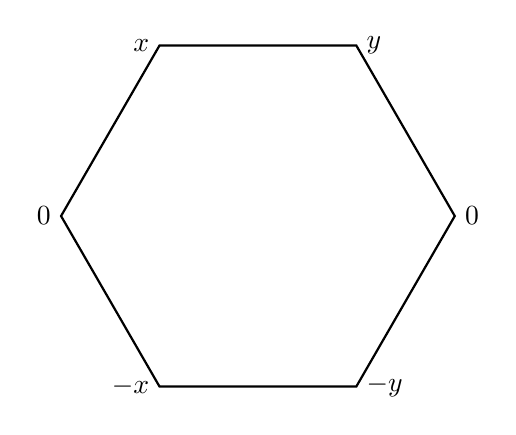
\begin{tikzpicture}[>=angle 90,scale=2.5]
\draw[thick]
(0,0) node[below,left]{$-x$}
-- ++(0:1) node[below,right]{$-y$}
-- ++(60:1) node[right]{$0$}
-- ++(120:1) node[above,right]{$y$}
-- ++(180:1) node[above,left]{$x$}
-- ++(240:1) node[left]{$0$}
-- cycle;
\end{tikzpicture}
%\hrule
%\vskip .15in
%\medskip
\end{figure}

%\medskip
%DIAGRAM6
%\sh{-25}{\box\boxF}
%\medskip

\noindent $B_2$  The corners of the squares represent the long roots
and the midedges represent the short roots

\begin{figure}[htb]
\centering
\begin{tikzpicture}[>=angle 90,scale=2.5]
\node[text width=2cm,align=justify] at (0,0.35) {
B.I\par
$a+b+c=0$
};
\draw[thick]
(0,0) node[above,left]{$y$}
-- ++(0:0.5) node[above]{$a$}
-- ++(0:0.5) node[above,right]{$0$}
-- ++(270:0.5) node[right]{$c$}
-- ++(270:0.5) node[below,right]{$0$}
-- ++(180:0.5) node[below]{$b$}
-- ++(180:0.5) node[below,left]{$-y$}
-- ++(90:0.5) node[left]{$0$}
-- cycle;

\node[text width=2cm,align=justify] at (2.5,0.35) {
B.II\par
$a+b+c=0$
};
\draw[thick]
(2.5,0) node[above,left]{$a$}
-- ++(0:0.5) node[above]{$0$}
-- ++(0:0.5) node[above,right]{$c$}
-- ++(270:0.5) node[right]{$-x$}
-- ++(270:0.5) node[below,right]{$0$}
-- ++(180:0.5) node[below]{$x$}
-- ++(180:0.5) node[below,left]{$b$}
-- ++(90:0.5) node[left]{$0$}
-- cycle;

\node[text width=2cm,align=justify] at (0,-1.65) {
B.III
};
\draw[thick]
(0,-2.0) node[above,left]{$y$}
-- ++(0:0.5) node[above]{$x$}
-- ++(0:0.5) node[above,right]{$z$}
-- ++(270:0.5) node[right]{$0$}
-- ++(270:0.5) node[below,right]{$-z$}
-- ++(180:0.5) node[below]{$-x$}
-- ++(180:0.5) node[below,left]{$-y$}
-- ++(90:0.5) node[left]{$0$}
-- cycle;

\node[text width=2cm,align=justify] at (2.5,-1.65) {
B.IV
};
\draw[thick]
(2.5,-2.0) node[above,left]{$y$}
-- ++(0:0.5) node[above]{$x$}
-- ++(0:0.5) node[above,right]{$0$}
-- ++(270:0.5) node[right]{$-x$}
-- ++(270:0.5) node[below,right]{$-y$}
-- ++(180:0.5) node[below]{$-z$}
-- ++(180:0.5) node[below,left]{$0$}
-- ++(90:0.5) node[left]{$z$}
-- cycle;

\end{tikzpicture}
%\hrule
%\vskip .15in
%\medskip
\end{figure}

%\medskip
%DIAGRAM7
%\sh{-20}{\box\boxG}
%\medskip

\newpage
\noindent $G_2$  The corners of the hexagon represent the long roots
and the midedges represent the short roots.
%\nobreak
%DIAGRAM8
%\sh{-30}{\box\boxH}
%\medskip

\begin{figure}[htb]
\centering
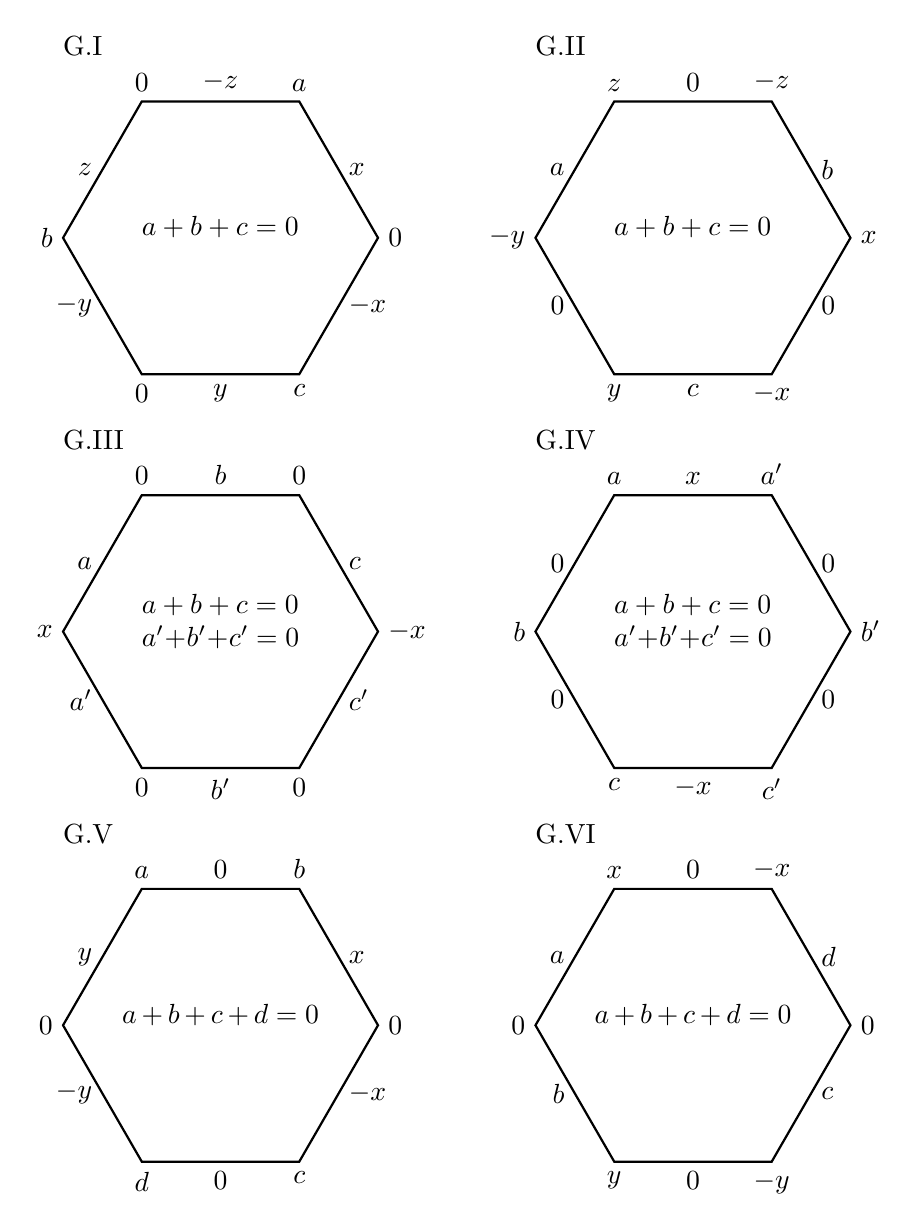
\begin{tikzpicture}[>=angle 90,scale=2]
\node[text width=2cm,align=justify] at (0,0.35) {
G.I
};
\node[text width=2cm,align=justify] at (0.5,-0.8) {
$a+b+c=0$
};
\draw[thick]
(0,0) node[above]{$0$}
-- ++(0:0.5) node[above]{$-z$}
--  ++(0:0.5) node[above]{$a$}
--  ++(-60:0.5) node[above,right]{$x$} 
--  ++(-60:0.5) node[right]{$0$} 
--  ++(-120:0.5) node[below,right]{$-x$}
--  ++(-120:0.5) node[below]{$c$}
--  ++(180:0.5) node[below]{$y$}
--  ++(180:0.5) node[below]{$0$}
-- ++(-240:0.5) node[below,left]{$-y$}
-- ++(-240:0.5) node[left]{$b$}
-- ++(60:0.5) node[above,left]{$z$}
--cycle;
% GII
\node[text width=2cm,align=justify] at (3+0,0.35) {
G.II
};
\node[text width=2cm,align=justify] at (3+0.5,-0.8) {
$a+b+c=0$
};
\draw[thick]
(3,0) node[above]{$z$}
-- ++(0:0.5) node[above]{$0$}
--  ++(0:0.5) node[above]{$-z$}
--  ++(-60:0.5) node[above,right]{$b$} 
--  ++(-60:0.5) node[right]{$x$} 
--  ++(-120:0.5) node[below,right]{$0$}
--  ++(-120:0.5) node[below]{$-x$}
--  ++(180:0.5) node[below]{$c$}
--  ++(180:0.5) node[below]{$y$}
-- ++(-240:0.5) node[below,left]{$0$}
-- ++(-240:0.5) node[left]{$-y$}
-- ++(60:0.5) node[above,left]{$a$}
--cycle;
% GIII
\node[text width=2cm,align=justify] at (0*3+0,0.35 -2.5) {
G.III
};
\node[text width=2cm,align=justify] at (0*3+0.5,-0.8 -2.5) {
$a+b+c=0$\par
$a'+b'+c'=0$
};
\draw[thick]
(0*3,-2.5) node[above]{$0$}
-- ++(0:0.5) node[above]{$b$}
--  ++(0:0.5) node[above]{$0$}
--  ++(-60:0.5) node[above,right]{$c$} 
--  ++(-60:0.5) node[right]{$-x$} 
--  ++(-120:0.5) node[below,right]{$c'$}
--  ++(-120:0.5) node[below]{$0$}
--  ++(180:0.5) node[below]{$b'$}
--  ++(180:0.5) node[below]{$0$}
-- ++(-240:0.5) node[below,left]{$a'$}
-- ++(-240:0.5) node[left]{$x$}
-- ++(60:0.5) node[above,left]{$a$}
--cycle;
% GIV
\node[text width=2cm,align=justify] at (1*3+0,0.35 -2.5) {
G.IV
};
\node[text width=2cm,align=justify] at (1*3+0.5,-0.8 -2.5) {
$a+b+c=0$\par
$a'+b'+c'=0$
};
\draw[thick]
(1*3,-2.5) node[above]{$a$}
-- ++(0:0.5) node[above]{$x$}
--  ++(0:0.5) node[above]{$a'$}
--  ++(-60:0.5) node[above,right]{$0$} 
--  ++(-60:0.5) node[right]{$b'$} 
--  ++(-120:0.5) node[below,right]{$0$}
--  ++(-120:0.5) node[below]{$c'$}
--  ++(180:0.5) node[below]{$-x$}
--  ++(180:0.5) node[below]{$c$}
-- ++(-240:0.5) node[below,left]{$0$}
-- ++(-240:0.5) node[left]{$b$}
-- ++(60:0.5) node[above,left]{$0$}
--cycle;
% GV
% GV
\node[text width=2cm,align=justify] at (0*3+0,0.35 -2.5*2) {
G.V
};
\node[text width=2.5cm,align=justify] at (0*3+0.5,-0.8 -2.5*2) {
$a+b+c+d=0$
};
\draw[thick]
(0*3,-2.5*2) node[above]{$a$}
-- ++(0:0.5) node[above]{$0$}
--  ++(0:0.5) node[above]{$b$}
--  ++(-60:0.5) node[above,right]{$x$} 
--  ++(-60:0.5) node[right]{$0$} 
--  ++(-120:0.5) node[below,right]{$-x$}
--  ++(-120:0.5) node[below]{$c$}
--  ++(180:0.5) node[below]{$0$}
--  ++(180:0.5) node[below]{$d$}
-- ++(-240:0.5) node[below,left]{$-y$}
-- ++(-240:0.5) node[left]{$0$}
-- ++(60:0.5) node[above,left]{$y$}
--cycle;
% GVI
\node[text width=2cm,align=justify] at (1*3+0,0.35 -2.5*2) {
G.VI
};
\node[text width=2.5cm,align=justify] at (1*3+0.5,-0.8 -2.5*2) {
$a+b+c+d=0$
};
\draw[thick]
(1*3,-2.5*2) node[above]{$x$}
-- ++(0:0.5) node[above]{$0$}
--  ++(0:0.5) node[above]{$-x$}
--  ++(-60:0.5) node[above,right]{$d$} 
--  ++(-60:0.5) node[right]{$0$} 
--  ++(-120:0.5) node[below,right]{$c$}
--  ++(-120:0.5) node[below]{$-y$}
--  ++(180:0.5) node[below]{$0$}
--  ++(180:0.5) node[below]{$y$}
-- ++(-240:0.5) node[below,left]{$b$}
-- ++(-240:0.5) node[left]{$0$}
-- ++(60:0.5) node[above,left]{$a$}
--cycle;
\end{tikzpicture}
%\hrule
%\vskip .15in
%\medskip
\end{figure}
%\box \boxD
%\newpage

% Second batch of G figures:
\begin{figure}[htb]
\centering
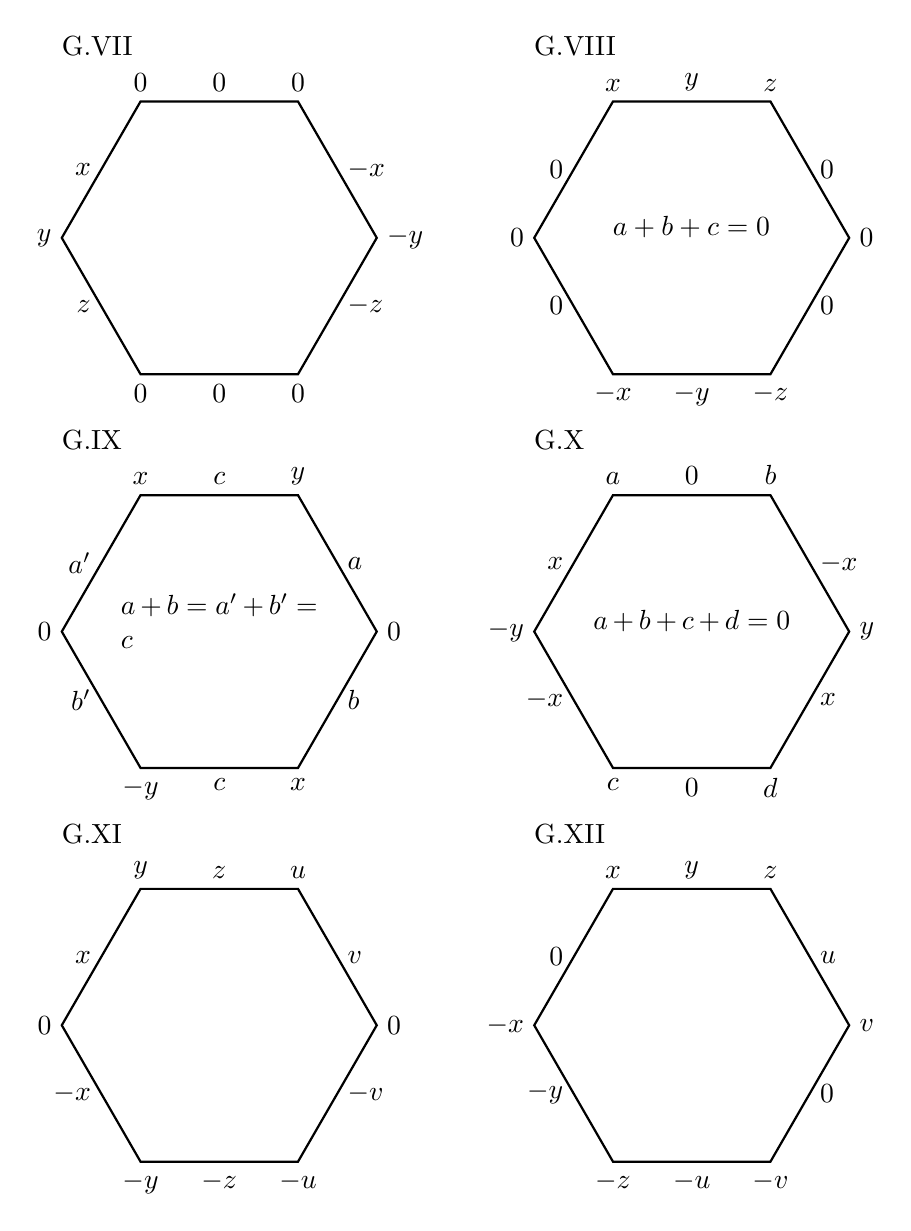
\begin{tikzpicture}[>=angle 90,scale=2]
\node[text width=2cm,align=justify] at (0,0.35) {
G.VII
};
\draw[thick]
(0,0) node[above]{$0$}
-- ++(0:0.5) node[above]{$0$}
--  ++(0:0.5) node[above]{$0$}
--  ++(-60:0.5) node[above,right]{$-x$} 
--  ++(-60:0.5) node[right]{$-y$} 
--  ++(-120:0.5) node[below,right]{$-z$}
--  ++(-120:0.5) node[below]{$0$}
--  ++(180:0.5) node[below]{$0$}
--  ++(180:0.5) node[below]{$0$}
-- ++(-240:0.5) node[below,left]{$z$}
-- ++(-240:0.5) node[left]{$y$}
-- ++(60:0.5) node[above,left]{$x$}
--cycle;
% GVIII
\node[text width=2cm,align=justify] at (3+0,0.35) {
G.VIII
};
\node[text width=2cm,align=justify] at (3+0.5,-0.8) {
$a+b+c=0$
};
\draw[thick]
(3,0) node[above]{$x$}
-- ++(0:0.5) node[above]{$y$}
--  ++(0:0.5) node[above]{$z$}
--  ++(-60:0.5) node[above,right]{$0$} 
--  ++(-60:0.5) node[right]{$0$} 
--  ++(-120:0.5) node[below,right]{$0$}
--  ++(-120:0.5) node[below]{$-z$}
--  ++(180:0.5) node[below]{$-y$}
--  ++(180:0.5) node[below]{$-x$}
-- ++(-240:0.5) node[below,left]{$0$}
-- ++(-240:0.5) node[left]{$0$}
-- ++(60:0.5) node[above,left]{$0$}
--cycle;
% GIX
\node[text width=2cm,align=justify] at (0*3+0,0.35 -2.5) {
G.IX
};
\node[text width=2.5cm,align=justify] at (0*3+0.5,-0.8 -2.5) {
$a+b=a'+b'=c$
};
\draw[thick]
(0*3,-2.5) node[above]{$x$}
-- ++(0:0.5) node[above]{$c$}
--  ++(0:0.5) node[above]{$y$}
--  ++(-60:0.5) node[above,right]{$a$} 
--  ++(-60:0.5) node[right]{$0$} 
--  ++(-120:0.5) node[below,right]{$b$}
--  ++(-120:0.5) node[below]{$x$}
--  ++(180:0.5) node[below]{$c$}
--  ++(180:0.5) node[below]{$-y$}
-- ++(-240:0.5) node[below,left]{$b'$}
-- ++(-240:0.5) node[left]{$0$}
-- ++(60:0.5) node[above,left]{$a'$}
--cycle;
% GX
\node[text width=2cm,align=justify] at (1*3+0,0.35 -2.5) {
G.X
};
\node[text width=2.5cm,align=justify] at (1*3+0.5,-0.8 -2.5) {
$a+b+c+d=0$
};
\draw[thick]
(1*3,-2.5) node[above]{$a$}
-- ++(0:0.5) node[above]{$0$}
--  ++(0:0.5) node[above]{$b$}
--  ++(-60:0.5) node[above,right]{$-x$} 
--  ++(-60:0.5) node[right]{$y$} 
--  ++(-120:0.5) node[below,right]{$x$}
--  ++(-120:0.5) node[below]{$d$}
--  ++(180:0.5) node[below]{$0$}
--  ++(180:0.5) node[below]{$c$}
-- ++(-240:0.5) node[below,left]{$-x$}
-- ++(-240:0.5) node[left]{$-y$}
-- ++(60:0.5) node[above,left]{$x$}
--cycle;
% GXI
% GXI
\node[text width=2cm,align=justify] at (0*3+0,0.35 -2.5*2) {
G.XI
};
\draw[thick]
(0*3,-2.5*2) node[above]{$y$}
-- ++(0:0.5) node[above]{$z$}
--  ++(0:0.5) node[above]{$u$}
--  ++(-60:0.5) node[above,right]{$v$} 
--  ++(-60:0.5) node[right]{$0$} 
--  ++(-120:0.5) node[below,right]{$-v$}
--  ++(-120:0.5) node[below]{$-u$}
--  ++(180:0.5) node[below]{$-z$}
--  ++(180:0.5) node[below]{$-y$}
-- ++(-240:0.5) node[below,left]{$-x$}
-- ++(-240:0.5) node[left]{$0$}
-- ++(60:0.5) node[above,left]{$x$}
--cycle;
% GXII
\node[text width=2cm,align=justify] at (1*3+0,0.35 -2.5*2) {
G.XII
};
\draw[thick]
(1*3,-2.5*2) node[above]{$x$}
-- ++(0:0.5) node[above]{$y$}
--  ++(0:0.5) node[above]{$z$}
--  ++(-60:0.5) node[above,right]{$u$} 
--  ++(-60:0.5) node[right]{$v$} 
--  ++(-120:0.5) node[below,right]{$0$}
--  ++(-120:0.5) node[below]{$-v$}
--  ++(180:0.5) node[below]{$-u$}
--  ++(180:0.5) node[below]{$-z$}
-- ++(-240:0.5) node[below,left]{$-y$}
-- ++(-240:0.5) node[left]{$-x$}
-- ++(60:0.5) node[above,left]{$0$}
--cycle;
\end{tikzpicture}
\end{figure}

%\hrule
%\vskip .15in
%\medskip
%\box \boxD
%\vfill\newpage
%\medskip
%DIAGRAM9
%\box\boxI
%\medskip

A few remarks on the diagrams are in order.  Consider first the case $A_{2}$.
Suppose $x_{2}=0$ for instance.   Then
$$
\e_\alpha(x_{1}){\e}_{\beta}(y_{1}+y_{2})
{\e}_{\alpha}(x_{3}){\e}_{\beta}(y_{3}) = 0.
$$
Lemma 1.3.b together with the fact that at least one variable of each
type must be non-zero implies that $y_{1}+y_{2}=y_{3}=0$.

Consider $B_{2}$.  Suppose $x_{3} = 0$.
 Then lemma 1.3.c together with the hypothesis that at least one wall of
type ${\alpha}$ is non-zero implies that $y_{1} = y_{2}+y_{3} = y_{4} = 0$
(pattern $B.I)$, or $x_{2} = x_{3} = y_{4} = 0$ if the $x_{i}$ of (1.3.c) is
adjacent to $x_{3}$ (pattern $B.II)$, or $x_{3} = x_{1} = y_{2}+y_{3} = 0$
if the $x_{i}$ of the lemma is not adjacent to $x_{2}$ (pattern $B.III)$.
 Finally suppose that none of the walls $x_{i}$ are zero.
 Then suppose $y_{1} = 0$.
 Again we apply (1.3.c) noting that the first two possibilities do not
arise, so that we have $x_{1}+x_{2} = y_{3} = 0$ (pattern $B.IV)$.

   I will not give a proof that the zero patterns listed above for $G_{2}$
are the only possibilities but I will make the results that follow independent
of this classification.

\section{Coordinate\ Relations}

   As a next step in the proof of proposition 1.1 it is necessary to obtain
formulas relating the functions $w({\g})$ to the coordinates
$z(W,{\alpha})$.   Lemmas 7.2 and 7.3 relate the coefficients $n_{\beta}$
to the coordinates $z(W,{\alpha})$.
 Thus it is enough to calculate the dependence of $w({\g})$ on the
coefficients $n_{\beta}$.
  Lemmas 2.1 and 2.2 carry out these calculations.

\medpagebreak

\begin{lemma}{Lemma 2.1}   Defining $a,b,c,d,e,f,g,h,i,j$ as in $(II.7)$ we have

$${\e}_{{\z}}(x_{{\z}}){\e}_{{\e}}(x_{{\e}})
{\e}_{{\delta}}(x_{{\delta}}){\e}_{{\g}}(x_{{\g}})
{\e}_{\beta}(x_{\beta}){\e}_{\alpha}(x_{\alpha})
$$  times      $$ {\e}_{\alpha}(y_{{\alpha }}){\e}_{\beta}(y_{\beta})
{\e}_{{\g}}(y_{{\g}}){\e}_{{\delta}}(y_{{\delta}})
{\e}_{{\e}}(y_{{\e}}){\e}_{{\z}}(y_\z)$$

$$
= {\e}_{\alpha}(z_{\alpha}){\e}_{\beta}(z_{\beta})
{\e}_{{\g}}(z_{{\g}}){\e}_{{\delta}}(z_{{\delta}})
{\e}_{{\e}}(z_{{\e}}){\e}_{{\z}}(z_{{\z}})
$$
with

\noindent
$z_{\alpha} = x_{\alpha}+y_{\alpha}$

\noindent
$z_{\beta} = x_{\beta}+y_{\beta}$

\noindent
$z_{{\g}} = x_{{\g}}+y_{{\g}} + a(x_{\alpha}+y_{\alpha})
x_{\beta}$

\noindent
$z_{{\delta}} = x_{{\delta}}+y_{{\delta}} + b(x_{\alpha}+y_{\alpha})^{2}
x_{\beta} + e(x_{\alpha}+y_{\alpha})x_{{\g}}$

\noindent
$z_{{\e}} = x_{{\e}}+y_{{\e}} + c(x_{\alpha}+
y_{\alpha})^{3}x_{\beta} + f(x_{\alpha}+y_{\alpha})^{2}x_{{\g}} +
h(x_{\alpha}+y_{\alpha})x_{{\delta}}$

\noindent
$z_{{\z}} = x_{{\z}}+y_{{\z}} + d(x_{\alpha}+y_{\alpha})^{3}
x_{\beta}^{2} + g(x_{\alpha}+y_{\alpha})x_{{\g}}^{2} + i(x_{\beta}
+y_{\beta})x_{{\e}} + j(x_{{\g}}+y_{{\g}})x_{{\delta}}$

   $+ hi(x_{\alpha}+y_{\alpha})(x_{\beta}+y_{\beta})x_{{\delta}} +
fi(x_{\alpha}+y_{\alpha})^{2}(x_{\beta}+y_{\beta})x_{{\g}} +
ci(x_{\alpha}+y_{\alpha})^{3}x_{\beta}y_{\beta}$

   $+ bj(x_{\alpha}+y_{\alpha})^{2}x_{\beta}y_{{\g}} +
ej(x_{\alpha}+y_{\alpha})x_{{\g}}y_{{\g}} + aj(x_{\alpha}+
y_{\alpha})x_{\beta}x_{{\delta}} + aje(x_{\alpha}+y_{\alpha})^{2}
x_{\beta}x_{{\g}}.$
\end{lemma}


\begin{proof}    The underlined quantities are moved to the left in each step.

${\e}_{{\z}}(x_{{\z}}){\e}_{{\e}}(x_{{\e}})
{\e}_{{\delta}}(x_{{\delta}}){\e}_{{\g}}(x_{{\g}})
{\e}_{\beta}(x_{\beta})$

$
% First term
{\underline{{\e}_{\alpha}(x_{\alpha}){\e}_{\alpha}(y_{\alpha})}}
{\e}_{\beta}(y_{\beta})
{\e}_{{\g}}(y_{{\g}}){\e}_{{\delta}}(y_{{\delta}})
{\e}_{{\e}}(y_{{\e}}){\e}_{{\z}}(y_{{\z}})=$

\medpagebreak

% Alpha term
${\e}_{\alpha}({ {x_{\alpha}+y_{\alpha}}}){\e}_{{\z}}
(x_{{\z}}){\e}_{{\e}}(x_{{\e}})
{ (}{\e}_{{\delta}}(x_{{\delta}}){\e}_{{\e}}
(h(x_{\alpha}+y_{\alpha})x_{{\delta}}){\e}_{{\g}}
(x_{{\g}}){\e}_{{\delta}}(e(x_{\alpha}+y_{\alpha})x_\g)$

${\e}_{{\e}}(f(x_{\alpha}+y_{\alpha})^{2}x_{{\g}})
{\e}_{{\z}}(g(x_{\alpha}+y_{\alpha})x_{{\g}}^{2}))
({\underline{{\e}_{\beta}(x_{\beta})}}
{\e}_{{\g}}(a(x_{\alpha}
+y_{\alpha})x_{\beta}){\e}_{{\delta}}(b(x_{\alpha}+
y_{\alpha})^{2}x_{\beta})$

${\e}_{{\e}}(c(x_{\alpha}+y_{\alpha})^{3}x_{\beta})
{\e}_{{\z}}(d(x_{\alpha}+y_{\alpha})^{3}x_{\beta}^{2}))\cdot
{\underline{{\e}_{\beta}(y_{\beta})}} {\e}_{{\g}}
(y_{{\g}}){\e}_{{\delta}}(y_{{\delta}}){\e}_{{\e}}
(y_{{\e}}){\e}_{{\z}}(y_{{\z}}) =$

\medpagebreak

% Alpha Beta term
${\e}_{\alpha}(z_{\alpha}){\e}_{\beta}({ x_{\beta}+
y_{\beta}}){\e}_{{\z}}(x_{{\z}}){ (}{\e}_{{\e}}
(x_{{\e}}){\e}_{{\z}}(i(x_{\beta}+y_{\beta})x_{{\e}})
{ )}{\e}_{{\delta}}(x_{{\delta}}){ (}{\e}_{{\e}}
(h(x_{\alpha}+y_{\alpha})x_\delta)$

$\e_\z(ih(x_\beta+y_\beta)(x_\alpha+y_\alpha)
x_{{\delta}})){\underline{{\e}_{{\g}}(x_{{\g}})}}
{\e}_{{\delta}} (e(x_{\alpha}+y_{\alpha})x_{{\g}})
({\e}_{{\e}}(f(x_{\alpha}+y_{\alpha})^{2}x_{{\g}})$

${\e}_{{\z}}(fi(x_{\alpha}+y_{\alpha})^{2}(x_{\beta}+y_{\beta})
x_{{\g}}) { ) }{\e}_{{\z}}(g(x_{\alpha}+y_{\alpha})
x_{{\g}}^{2}) \cdot $

$
{\underline{{\e}_{{\g}}(a(x_{\alpha}+y_{\alpha})x_{\beta})}}
{\e}_{{\delta}}(b(x_{\alpha}+y_{\alpha})^{2}x_{\beta})$

$({\e}_{{\e}}(c(x_{\alpha}+y_{\alpha})^{3}x_{\beta})
{\e}_{{\z}}(ci(x_{\alpha}+y_{\alpha})^{3}x_{\beta}y_{\beta})
{ )}{\e}_{{\z}}(d(x_{\alpha}+y_{\alpha})^{3}x_{\beta}^{2})
\cdot {\underline{{\e}_{{\g}}(y_{{\g}})}}
{\e}_{{\delta}}(y_{{\delta}})$

${\e}_{{\e}}(y_{{\e}}){\e}_{{\z}}(y_{{\z}}) = $

\medpagebreak

% Alpha Beta Gamma term
$\e_\alpha(z_\alpha)\e_\beta(z_\beta)
{\e}_{{\g}}({ x_{{\g}}+y_{{\g}}+a(x_{\alpha}+
y_{\alpha})x_{\beta}}){\e}_{{\z}}(x_{{\z}})
{\e}_{{\e}}(x_{{\e}}){\e}_{{\z}}(i(x_{\beta}+
y_{\beta})x_{{\e}})$

${\underline{({\e}_{{\delta}}
(x_{\delta})}}{\e}_{{\z}}(j(x_{{\g}}+y_{{\g}})x_{{\delta}}+aj(x_{\alpha}+
y_{\alpha})x_{\beta}x_{{\delta}}){ )}$

${\e}_{{\e}}
(h(x_{\alpha}+y_{\alpha})x_{{\delta}}){\e}_{{\z}}(ih(x_{\beta}+
y_{\beta})(x_{\alpha}+y_{\alpha})x_{\delta})\cdot$

${\underline{{\e}_{{\delta}}(e(x_{\alpha}+y_{\alpha})x_{{\g}})}}
{\e}_{{\z}}(ej(x_{\alpha}+y_{\alpha})y_{{\g}}x_{{\g}}+
aje(x_{\alpha}+y_{\alpha})^{2}x_{\beta}x_{{\g}}){ )}
{\e}_{{\e}}(f(x_{\alpha}+y_{\alpha})^{2}x_{{\g}})$

${\e}_{{\z}}(fi(x_{\alpha}+y_{\alpha})^{2}(x_{\beta}+
y_{\beta})x_{{\g}}){\e}_{{\z}}(g(x_{\alpha}+y_{\alpha})
x_{{\g}}^{2})\cdot ({\underline{{\e}_{{\delta}}(b(x_{\alpha}
+y_{\alpha}) ^{2} x_{\beta})}}$


${\e}_{{\z}}(bj(x_{\alpha}+y_{\alpha})^{2}x_{\beta}y_{{\g}})
{ )}{\e}_{{\e}}(c(x_{\alpha}+y_{\alpha})^{3}x_{\beta})
{\e}_{{\z}}(ci(x_{\alpha}+y_{\alpha})^{3}x_{\beta}y_{\beta})$


${\e}_{{\z}}(d(x_{\alpha}+y_{\alpha})^{3}x_{\beta}^{2}) \cdot
{\underline{{\e}_{{\delta}}(y_{{\delta}})}} {\e}_{{\e}}
(y_{{\e}}){\e}_{{\z}}(y_{{\z}}) =$

\medpagebreak


$\e_\alpha(z_{\alpha})\e_\beta(z_\beta)
\e_\g(z_\g)\e_\delta( x_\delta+y_\delta+b(x_\alpha+y_\alpha)^2x_\beta+e(x_\alpha+
y_\alpha)x_\g)\e_\z(x_\z)
{\underline{\e_\e(x_\e)}}$



${\e}_{{\z}}(i(x_{\beta}+y_{\beta})x_{{\e}})\cdot
{\e}_{{\z}}(j(x_{{\g}}+y_{{\g}})x_{{\delta}}+
aj(x_{\alpha}+y_{\alpha})x_{\beta}x_{{\delta}})
{\underline{{\e}_{{\e}}(h(x_{\alpha}+
y_{\alpha})x_{{\delta}})}}$

${\e}_{{\z}}(ih(x_{\beta}+y_{\beta})(x_{\alpha}+y_{\alpha})
x_{{\delta}})$

${\e}_{{\z}}(ej(x_{\alpha}+y_{\alpha})
y_{{\g}}x_{{\g}}+aje(x_{\alpha}+y_{\alpha})^{2}x_{\beta}
x_\g){\underline{\e_{{\e}}(f(x_{\alpha}+
y_\alpha)^2 x_\g)}}$

${\e}_{{\z}}(fi(x_{\alpha}+y_{\alpha})^{2}(x_{\beta}+
y_{\beta})x_{{\g}}){\e}_{{\z}}(g(x_{\alpha}+y_{\alpha})
x_{{\g}}^{2})$

${\e}_{{\z}}(bj(x_{\alpha}+
y_{\alpha})^{2}x_{\beta}y_{{\g}})
{\underline{{\e}_{{\e}}(c(x_{\alpha}+y_{\alpha}) ^{3}x_{\beta})}}$

${\e}_{{\z}}(ci(x_{\alpha}+y_{\alpha})^{3}x_{\beta}y_{\beta})
{\e}_{{\z}}(d(x_{\alpha}+y_{\alpha})^{3}x_{\beta}^{2}) \cdot
{\underline{{\e}_{{\e}}(y_{{\e}})
{\e}_{{\z}}(y_{{\z}})}} =$

\medpagebreak

$\e_\alpha(z_\alpha)\e_\beta(z_\beta)
{\e}_{{\g}}(z_{{\g}}){\e}_{{\delta}}(z_{{\delta}})$

${\e}_{{\e}}( x_{{\e}}+y_{{\e}}+c(x_{\alpha}+
y_{\alpha})^{3}x_{\beta}+f(x_{\alpha}+y_{\alpha})^{2}x_{{\g}}+
h(x_{\alpha}+y_{\alpha})x_{{\delta}})$

${\e}_{{\z}}(x_{{\z}}) \cdot {\e}_{{\z}}
(i(x_{\beta}+y_{\beta})x_{{\e}}){\e}_{{\z}}(j(x_{{\g}}+
y_{{\g}})x_{{\delta}}+aj(x_{\alpha}+y_\alpha)x_{\beta}x_{{\delta}})
$

${\e}_{{\z}}(ih(x_{\beta}+y_{\beta})(x_{\alpha}+
y_{\alpha})x_{{\delta}})$

${\e}_{{\z}}(ej(x_{\alpha}+y_{\alpha})y_{{\g}}x_{{\g}}+
aje(x_{\alpha}+y_{\alpha})^{2}x_{\beta}x_{{\g}})$

$
{\e}_{{\z}}(fi(x_{\alpha}+y_{\alpha})^{2}(x_{\beta}+y_{\beta})
x_{{\g}}){\e}_{{\z}}(g(x_{\alpha}+y_{\alpha})x_{{\g}}^2)$

${\e}_{{\z}}(bj(x_{\alpha}+y_{\alpha})^{2}x_{\beta}y_{{\g}})
\cdot {\e}_{{\z}}(ci(x_{\alpha}+y_{\alpha})^{3}
x_{\beta}y_{\beta}){\e}_{{\z}}(d(x_{\alpha}+y_{\alpha})^{3}
x_{\beta}^{2}) \cdot {\e}_{{\z}}(y_{\z}) =$

\medpagebreak


${\e}_{\alpha}(z_{\alpha}){\e}_{\beta}(z_{\beta})
{\e}_{{\g}}(z_{{\g}}){\e}_{{\delta}}(z_{{\delta}})
{\e}_{{\e}}(z_{{\e}})$

${\e}_{{\z}}(x_{{\z}} + i(x_{\beta}+y_{\beta})x_{{\e}} +
j(x_{{\g}}+y_{{\g}})x_{{\delta}} + aj(x_{\alpha}+y_{\alpha})
x_{\beta}x_{{\delta}} + ih(x_{\beta}+y_{\beta})(x_{\alpha}+y_{\alpha})
x_{{\delta}})$

${\e}_{{\z}}(ej(x_{\alpha}+y_{\alpha})y_{{\g}}x_{{\g}} +
aje(x_{\alpha}+y_{\alpha})^{2}x_{\beta}x_{{\g}} + $

$\qquad\qquad\qquad\qquad
fi(x_{\alpha}+ y_\alpha)^2(x_\beta+y_\beta)x_\g + g(x_\alpha+ y_\alpha)x_\g^2)$

${\e}_{{\z}}(bj(x_{\alpha}+y_{\alpha})^{2}x_{\beta}y_{{\g}}
+ ci(x_{\alpha}+y_{\alpha})^{3}x_{\beta}y_{\beta} +
d(x_{\alpha}+y_{\alpha})^{3}x_{\beta}^{2} + y_{{\z}})$.
\hfill
\end{proof}
{\medskip}


\begin{corollary}{Corollary 2.2}   $t^{-1}n^{-1}tn =$
$${\e}_{\alpha}(x({\alpha})){\e}_{\beta}(x({\beta}))
{\e}_{{\g}}(x({\g})){\e}_{{\delta}}(x({\delta}))
{\e}_{{\e}}(x({\e})){\e}_{{\z}}(x({\z}))$$

\noindent
where

$n = {\e}_{\alpha}(n_{\alpha}){\e}_{\alpha}
(n_{\alpha}){\e}_{\beta}(n_{\beta}){\e}_{{\g}}
(n_{{\g}}){\e}_{{\delta}}(n_{{\delta}}){\e}_{{\z}}
(n_{{\z}})$

$x({\alpha}) = (1-{\alpha}^{-1})n_{\alpha}$

$x({\beta}) = (1-{\beta}^{-1})n_{\beta}$

$x({\g}) = (1-{\g}^{-1})n_{{\g}} -a(1-{\alpha}^{-1}){\beta}^{-1}
n_{\alpha}n_{\beta}$

$x({\delta}) = (1-{\delta}^{-1})n_{{\delta}} -b(1-{\alpha}^{-1})^{2}
{\beta}^{-1}n_{\alpha}^{2}n_{\beta} -e(1-{\alpha}^{-1}){\g}^{-1}
n_{\alpha}n_{{\g}}$

$x({\e}) = (1-{\e}^{-1})n_{{\e}} -c(1-{\alpha}^{-1})^{3}
{\beta}^{-1}n_{\alpha}^{3}n_{\beta} -f(1-{\alpha}^{-1})^{2}{\g}^{-1}
n_{\alpha}n_{{\g}}$

\quad     $-h(1-{\alpha}^{-1}){\delta}^{-1}n_{\alpha}n_{{\delta}}$


$x({\z}) = (1-{\z}^{-1})n_{{\z}} + d(1-{\alpha}^{-1})^{3}{\beta}^{-2}
n_{\alpha}^{3}n_{\beta}^{2} + g(1-{\alpha}^{-1}){\g}^{-2}n_{\alpha}
n_{{\g}}^{2}$


\quad    $-i(1-{\beta}^{-1}){\e}^{-1}n_{\beta}n_{{\e}} -
j(1-{\g}^{-1}){\delta}^{-1}n_{{\g}}n_{{\delta}}$

\quad  $-hi(1-{\alpha}^{-1})(1-{\beta}^{-1}){\delta}^{-1}n_{\alpha}n_{\beta}
n_{{\delta}}$

\quad   $-fi(1-{\alpha}^{-1})^{2}(1-{\beta}^{-1}){\g}^{-1}n_{\alpha}^{2}
n_{\beta}n_{{\g}} -ci(1-{\alpha}^{-1})^{3}{\beta}^{-1}n_{\alpha}^{3}
n_{\beta}^{2}$

\quad    $-bj(1-{\alpha}^{-1})^{2}{\beta}^{-1}n_{\alpha}^{2}n_{\beta}
n_{{\g}} -ej(1-{\alpha}^{-1}){\g}^{-1}n_{\alpha}n_{{\g}}^{2}$

\quad    $+aj(1-{\alpha}^{-1}){\beta}^{-1}{\delta}^{-1}n_{\alpha}n_{\beta}
n_{{\delta}} +aje(1-{\alpha}^{-1})^{2}{\beta}^{-1}{\g}^{-1}n_{\alpha}^{2}
n_{\beta}n_{{\g}}$.
\end{corollary}

\begin{proof}    Let $x_{{\eta}} = -n_{{\eta}}{\eta}^{-1}, y_{{\eta}} =
n_{{\eta}}$ in the previous lemma for ${\eta} =$
${\alpha}$, ${\beta}$, ${\g}$, ${\delta}$, ${\e}$, ${\z}$.
\end{proof}

{\medskip}

In the next lemma we gather together equations that will be used to prove
the main result of this section.

\begin{lemma}{Lemma 2.3}   The following equations hold on $Y''$.
\begin{enumerate}[label=(\alph*)]
\item $w({\alpha}) = 1, w({\beta}) = 1$
\item $n_{\alpha} = 1/z(W_{+},{\alpha}), n_{\beta} =
1/z(W_{+},{\beta})$,
\item ${\lambda} = x({\alpha})z({\alpha}), {\lambda} =
x({\beta})z({\beta})$
\item $(1-{\alpha}^{-1}) = x({\alpha})z(W_{+},{\alpha}),
(1-{\beta}^{-1}) = x({\beta})z(W_{+},{\beta})$
\item $z(W_{+},{\alpha})/z({\alpha}) = z_{1}(W_{+},{\alpha}) =
(1-{\alpha}^{-1})/{\lambda}$
\item[] $z(W_{+},{\beta})/z({\beta}) = z_{1}(W_{+},{\beta}) =
(1-{\beta}^{-1})/{\lambda}$
\item $u_{2}'n_{{\g}} = -1/(z(W_{+},{\beta})z(W({\sigma}_{\beta}),
{\alpha}))$ where ${\sigma}_{\beta}(X_{{\g}}) = u_{2}'X_{\alpha}$
\item $$\aligned
{\lambda}w({\g}) &= z({\alpha})z({\beta})x({\g}) \\
&=
z({\alpha})z({\beta})((1-{\g}^{-1})n_{{\g}} - {\beta}^{-1}
(1-{\alpha}^{-1})n_{\alpha}n_{\beta})
\\ &=
[{\lambda}^{2}/(1-{\alpha}^{-1})(1-{\beta}^{-1})] \quad
\hbox{times}\\
&\quad\quad [(-(1-{\g}^{-1})
u_{2}^{\prime-1}z(W_+,{\alpha})/z(W({\sigma}_{\beta}),{\alpha})) -
{\beta}^{-1}(1-{\alpha}^{-1})]\endaligned$$
\end{enumerate}
\end{lemma}

\medpagebreak

\begin{proof}    (a) holds by definition.  (b) was proved in (I.5.5).
(c) are the defining relations for $z({\alpha})$ and $z({\beta})$.
(d) is equation (II.3.3) combined with (b).
In (e) the first equality on each line serves as the definition of
$z_{1}(W,-)$.
 The second equality on each line is obtained by dividing (d) by (c).
(f) was proved for $G_{2}$ in (II.7.2), (II.7.3).
 This calculation only makes use of the fact that ${\beta}$ is at least as
long as ${\alpha}$,
so that the calculation holds for $A_{2}$ and $B_{2}$ as well.
 This is consistent with (II.8.1) when ${\alpha} = {\beta}_{2},
{\beta}={\beta}_{1}, u_{2}'=-1$.
 The first equality of (g) is (II.4.2).
 The second equality is (2.2).
 This is consistent with (II.5.1).
 The third equality of (g) follows by using (e) for $z({\alpha})$ and
$z({\beta}), (f)$ for $n_{{\g}}$, and (b) for $n_{\alpha}n_{\beta}$.
\end{proof}

{\medskip}

\begin{lemma}{Lemma 2.4}    Let $dx_{1}\ldots dx_{n}$ be a form of maximal degree on
$Y_{{\Gamma}}$.
 Suppose that there are coordinates ${\mu}_{1},\ldots ,{\mu}_{n}$ on
$Y_{{\Gamma}}$ such that locally ${\mu}_{1} = 0$ defines a divisor $E$ and
$x_{i} = {\mu}_{1}^{a_i} {\xi}_{i}$ where ${\xi}_{i}$ is regular on $E$.
 Let $a = \sum a_{i}$.
 Then $dx_{1}\ldots dx_{n}$ vanishes to order at least $a-1$ on $E$.
\end{lemma}

\medpagebreak

\begin{proof}
$$
dx_1\ldots dx_n = {\frac{\partial(x_1,\ldots, x_n)}{\partial (\mu_1,\ldots,
\mu_n)}}\  d{\mu}_{1}\ldots d{\mu}_{n}.
$$

\noindent
Expanding the Jacobian by the first row we obtain
$$
{\frac{\partial(x_1,\ldots,x_n)}{\partial(\mu_1,\ldots,\mu_n)}} =\
\sum (\pm 1)\ {\frac{\partial x_i}{\partial \mu_1}}\
{\frac{\partial(x_1,\ldots,\hat{x}_i,\ldots,x_n)}{\partial(\mu_2,\ldots,\mu_n)}}.
$$
Now
$$
{\frac{\partial(x_1,\ldots,\hat{x}_i,\ldots,x_n)}{\partial(\mu_2,\mu_3,\ldots,\mu_n)}} =
\mu_1^{a-a_i}\ {\frac{\partial(\xi_1,\ldots,\hat{\xi}_i,\ldots,\xi_n)}
{\partial(\mu_2,\mu_3,\ldots,\mu_n)}}
$$
and
$$
{\frac{\partial x_i}{\partial \mu_1}} = a_i\mu_1^{a_i-1} \xi_i +
\mu_1^{a_i} {\frac{\partial\xi_i}{\partial \mu_1}} =
\mu_1^{a_i-1} (a_i\xi_i+\mu_1 {\frac{\partial \xi_i}{\partial \mu_1}}).
$$
Thus every term of the sum vanishes to order at least $(a-a_{i}) + (a_{i}-1)
= a-1$.
\end{proof}

\section{Exclusion\ of\ Spurious\ Divisors}


   The next few lemmas show that divisors with certain zero patterns make
no contribution to the subregular germ.
 $A$ subregular unipotent element is one whose centralizer has dimension
$rank(G)+2$.
 The proofs follow similar lines.
 Let $E$ be a divisor.
 If ${\lambda}$ vanishes to order ${a}$ on $E$ and the form
${\omega}_{Y}$ vanishes to order ${b-1}$ on $E$ then $E$ makes a
contribution to a term $m({\lambda})^{r}{\theta}({\lambda})\vert
{\lambda}\vert ^{{\beta}-1}F_{r}({\theta},{\beta},f)$ of the asymptotic
expansion with ${\beta}=b/a$.
 For details see \cite{MR701566}.

 Suppose we can express ${\omega}_{Y}$ locally as ${\lambda}^{2}{\mu}^{x}
 (d{\mu}/{\mu}) \wedge {\omega}'$ where $x>0, {\mu}$ is a local coordinate,
${\mu}=0$ defines $E$, and ${\omega}'$ regular on $E$.
 Then $b=2a+x, {\beta}-1 = (b/a)-1 = 1 + (x/a) > 1$.
 This shows that such a divisor $E$ does not contribute to the first order
term of the asymptotic expansion.
 By $(II.9.2)$, it does not contribute to the subregular germ.

   The coordinate functions $z(W,{\alpha})$ are regular on $Y_{1}(B_{{\infty}},
B_{0})$.
 However, it is rather awkward to work directly with these coordinates.
 On the variety $Y''$ we have seen in chapter II how to express the functions
$w({\g})$ in terms of $z({\alpha})$ \ (${\alpha}$ simple) and the coefficients
of $t$ and $n \ (II.3)$ and also how to express the coefficients of $n$ in terms
of the coordinates $z(W,{\alpha})$.
 Also $z({\alpha}) = ({\lambda}/(1-{\alpha}^{-1}))z(W_{+},{\alpha}) \
 (2.3)$.
 Thus on $Y''$ we can express $w({\eta})$ in terms of the coefficients of $t,
{\lambda}$ and $z(W,{\alpha})$.
 We use this expression to extend $w({\g})$ to a rational function on
$Y_{1}(B_{{\infty}},B_{0})$.
 Similarly we extend $n_{{\g}}$ to a rational function on
$Y_{1}(B_{{\infty}},B_{0})$.
 The following lemmas show that with appropriate hypotheses, $w({\eta})$ or
sometimes $1/w({\eta})$ may actually extend to a regular function on a Zariski
open set of certain spurious divisors.

   The next lemma does not assume that $G$ is rank two.

\medpagebreak

\begin{lemma}{Lemma 3.1}   Let $E$ be a divisor on $Y_{{\Gamma}}$.
 Suppose that $W_{+}$ and two simple adjacent roots ${\alpha}_{1}$ and
${\alpha}_{2}$ can be chosen so that ${\theta}_{1}(W_{+},{\alpha}_{1})\ne 0$,
and ${\theta}_{1}(W({\sigma}_{\alpha_2}),{\alpha}_{1}) = 0$ on $E$.
 Suppose also that the root ${\alpha}_{1}$ is not longer than the root
${\alpha}_{2}$.
 Then

\begin{enumerate}[label=\alph*)]
\item $1/w({\alpha}_{1}+{\alpha}_{2})$ is regular on $E$.
\item $1/w({\alpha}_{1}+{\alpha}_{2})$ vanishes on $E$.
\item $E$ makes no contribution to the subregular germ.
\end{enumerate}
\end{lemma}

\medpagebreak

\begin{proof}     Note that $z({\alpha}) = {\lambda}z(W_{+},{\alpha})/(1-{\alpha}^{-1})$
and $z({\beta}) = {\lambda}z(W_{+},{\beta})/(1-{\beta}^{-1})$ are regular on $E$.
 Set $w = 1/w({\alpha}_{1}+{\alpha}_{2})$.
 On $Y''$ we have by (2.3.g)
$w = [{\lambda}^{2}/(1-{\alpha}_{1}^{-1})(1-{\alpha}_{2}^{-1})]^{-1}$
$$
[(-(1-({\alpha}_{1}{\alpha}_{2})^{-1})/{\lambda})(u_{2}^{\prime-1}z(W_+,
{\alpha}_{1})/z(W({\sigma}_{\alpha_2}),{\alpha}_{1})) -
{\alpha}_{2}^{-1}(1-{\alpha}_{1}^{-1})/{\lambda}]^{-1} .
$$
Set $z = z(W({\sigma}_{\alpha_2}),{\alpha}_{1})/z(W_{+},{\alpha}_{1})$.
 By the hypotheses of the lemma, $z$ is regular on $E$ and is in fact equal to
zero on $E$.
 Thus up to a regular invertible factor, $w$ is equal to
$$
z[-((1-({\alpha}_{1}{\alpha}_{2})^{-1})/{\lambda})u_{2}^{\prime-1} -
z{\alpha}_{2}^{-1}(1-{\alpha}_{1}^{-1})/{\lambda}]^{-1} .
$$
Since $z = 0$ on $E$, the factor
$$
-((1-({\alpha}_{1}{\alpha}_{2}^{-1}))/{\lambda})u_{2}^{\prime-1} -
z{\alpha}_{2}^{-1}((1-{\alpha}_{1}^{-1})/{\lambda})
$$
equals $-((1-({\alpha}_{1}{\alpha}_{2})^{-1})/{\lambda})u_{2}^{\prime-1}$ on
$E$ and is consequently regular and invertible on $E$.
 Parts a) and b) follow.

   Formulas (2.3.c,g) give
$$
\aligned
x({\alpha}_{1}) &= {\lambda}/z({\alpha}_{1}) = z({\alpha}_{2})x({\alpha}_{1}
+{\alpha}_{2})w ,\ {\text{and}} \\
x({\alpha}_{2}) &= {\lambda}/z({\alpha}_{2}) = z({\alpha}_{1})x({\alpha}_{1}
+{\alpha}_{2})w , \\
{\lambda} &= z({\alpha}_{1})z({\alpha}_{2})x({\alpha}_{1}+{\alpha}_{2})w .
\endaligned
$$

     The form up to a factor we can ignore is given on $Y^{0}$ by

   $d{\lambda}\wedge dx({\alpha}_{1})\wedge dx({\alpha}_{2})\wedge
dx({\alpha}_{1}+{\alpha}_{2})\wedge \ldots d{\nu} = $

    ${\lambda}^{2}d{\lambda}\wedge d(1/z({\alpha}_{1}))\wedge
d(1/z({\alpha}_{2}))\wedge dx({\alpha}_{1}+{\alpha}_{2})\wedge
\ldots d{\nu} =$

$\lambda^{2}x({\alpha}_{1}+{\alpha}_{2})dw\wedge
(dz({\alpha}_{1})/z({\alpha}_{1}))\wedge (dz({\alpha}_{2})/z({\alpha}_{2}))
\wedge dx({\alpha}_{1}+{\alpha}_{2})\wedge \ldots d{\nu}$

\noindent
where
$$
d{\nu} = d{\nu}_{1}\wedge d{\nu}_{2}\wedge \ldots \wedge d{\nu}_{p} .
$$
Let ${\mu} = {\mu}_{1},\ldots , {\mu}_{n}$ be a coordinate system on
$Y_{{\Gamma}}$ near a point of $E$, and suppose that ${\mu} = 0$ defines the
divisor $E$ locally.
 Now pull the variables ${\lambda}, x({\alpha}_{1}+{\alpha}_{2}), w,
z({\alpha}_{1}), z({\alpha}_{2})$ etc.
up to $Y_{{\Gamma}}$ and write
$$
\aligned
z({\alpha}_{1}) &= {\mu}^{e_1} {\xi}_{1}\\
z({\alpha}_{2}) &= {\mu}^{e_2} {\xi}_{2} \\
x({\alpha}_{1}+{\alpha}_{2}) &= {\mu}^{e_3} {\xi}_{3} \\
w &= {\mu}^{e_4} {\xi}_{4}
\endaligned
$$
where ${\xi}_{i}$ is regular on $E$.
 By (2.4), $dw\wedge dz({\alpha}_{1})\wedge dz({\alpha}_{2})\wedge
dx({\alpha}_{1}+{\alpha}_{2})$ vanishes to order at least $e_{4}+e_{1}+
e_{2}+e_{3}-1$.
 Thus
$$
{\omega}_{Y} = {\lambda}^{2}{\mu}^{x}(d{\mu}/{\mu})\wedge {\omega}'
$$
where
$$
x \ge  (e_{3}-e_{1}-e_{2}) + (e_{4}+e_{1}+e_{2}+e_{3}-1) + 1
= 2e_{3}+e_{4} ,
$$
and ${\omega}'$ is regular on $E$.
 But $w$ vanishes on $E$ so $e_{4} > 0$.
 By remarks at the beginning of this section, the proof is complete.
\end{proof}
{\medskip}

\begin{lemma}{Lemma 3.2}\  ($B_{2}$)\ Suppose that the Weyl chamber $W_{+}$ can be
chosen on $E$ so that ${\theta}_{1}(W_{+},{\alpha})\ne 0, {\theta}_{1}(W_{+},
{\beta})\ne 0, {\theta}_{1}(W({\sigma}_{\beta}),{\alpha})\ne 0,
{\theta}_{1}(W({\sigma}_{\alpha}),{\beta}) = 0$.
 Then

\begin{enumerate}[label=\alph*)]
\item $w({\g})$ is regular on $E$,
\item $1/w({\delta})$ is regular on $E$ and in fact vanishes on $E$,
\item $E$ makes no contribution to the subregular germ.
\end{enumerate}
\end{lemma}

\begin{remark*} This lemma treats the zero pattern $B.IV$.
\end{remark*}

\medskip

\begin{proof} \   By (2.3.e)\  $z({\alpha}) = ({\lambda}/(1-{\alpha}^{-1}))z(W_{+},
{\alpha})$ and $$z({\beta})=({\lambda}/(1-{\beta}^{-1}))z(W_{+},{\beta}).$$
 Also by (2.3.b,f)
$$
n_{{\g}}/(n_{\alpha}n_{\beta}) = -u_{2}^{\prime-1}z(W_{+},
{\alpha})/z(W({\sigma}_{\beta}),{\alpha}) .
$$
Thus by the assumptions of the lemma $z({\alpha}), z({\beta})$, and
$n_{{\g}}/(n_{\alpha}n_{\beta})$ are regular.
 By (2.3.g)
$$
\aligned
w({\g}) &= z({\alpha})z({\beta})((1-{\g}^{-1})/{\lambda})n_{{\g}}
- {\beta}^{-1}((1-{\alpha}^{-1})/{\lambda})n_{\alpha}n_{\beta}) = \\
&= ({\lambda}^{2}/(1-{\alpha}^{-1})(1-{\beta}^{-1}))
(((1-{\g}^{-1})/{\lambda})(n_{{\g}}/(n_{\alpha}n_{\beta}) \\
&\quad\quad  - {\beta}^{-1}((1-{\alpha}^{-1})/{\lambda})).
\endaligned
$$
Thus the regularity of $n_{{\g}}/(n_{\alpha}n_{\beta})$ implies the
regularity of $w({\g})$.
 This proves (a).

   Let $z = z(W({\sigma}_{\alpha}),{\beta})/z(W_{+},{\beta})$.
 Then $z = 0$ on $E$ by assumption.
 By (II.3.3),
$$
\aligned
zw({\delta}) &= z(1-{\delta}^{-1})n_{{\delta}}z({\alpha})^{2}
z({\beta})/{\lambda} + zz({\alpha})^{2}z({\beta}) \sum
c_{\beta_1\ldots \beta_n}(t)n_{\beta_1}\ldots n_{\beta_n}/{\lambda}\\
z({\alpha}) &= {\lambda}/((1-{\alpha}^{-1})n_{\alpha}),
z({\beta}) = {\lambda}/((1-{\beta}^{-1})n_{\beta}).
\endaligned
$$
Thus
$$
zw({\delta}) = [{\lambda}^{3}/((1-{\alpha}^{-1})^{2}(1-{\beta}^{-1}))][zq +
(z(1-{\delta}^{-1})n_{{\delta}}/({\lambda}n_{\alpha}^{2}n_{\beta}))]
$$
where $q$ is the regular function $q = c_{{\alpha}{\alpha}{\beta}}(t)/{\lambda}
+ c_{{\alpha}{\g}}(t)n_{{\g}}/({\lambda}n_{\alpha}n_{\beta})$.
Since $q$ is regular on $E$ and $z = 0$ on $E, zq = 0$ on $E$.
If $zw({\delta})$ is regular and invertible on $E$ then $(b)$ will follow.
$\lambda^2(1-\delta^{-1})/((1-{\alpha}^{-1})^{2}(1-\beta^{-1}))$ is
regular and invertible on $E$ and $zq$ vanishes on $E$, so $zw({\delta})$ is
regular and invertible on $E$ if and only if $zn_{{\delta}}/(n_{\alpha}^{2}
n_{\beta})$ is regular and invertible on $E$.
 The following lemma completes the proof of (b).
\end{proof}

\medskip

\begin{lemma}{Lemma 3.3}\   $(B_{2})$\  Let $E$ be as in lemma 3.2.
 Then $zn_{{\delta}}/(n_{\alpha}^{2}n_{\beta})$ equals a non-zero constant
on $E$.
\end{lemma}

\begin{proof}    We apply the condition $B{\omega}n = Bn_{w}$ to the situation
${\omega} = {\sigma}_{\beta}{\sigma}_{\alpha}$ and
$$
\aligned
n_{w} &= \exp(z_{2}X_{-{\beta}})\exp(z_{1}X_{-{\alpha}}) \\
{\text{with}}\ z_{2} &= z(W({\sigma}_{\alpha}),{\beta}),
z_{1} = z(W_{+},{\alpha}).
\endaligned
$$
This condition can be rewritten
$$
{\sigma}_{\beta}{\sigma}_{\alpha}{\e}_{\alpha}(n_{\alpha})
{\e_\beta}(n_\beta)\e_\gamma(n_\gamma)\e_\delta(n_\delta)\e_{-\alpha}
(-z_{1}){\e}_{-{\beta}}(-z_{2}) \in B
$$
or
$$
\sigma_\beta
\{       \sigma_\alpha\e_\alpha(n_\alpha) \e_{-\alpha}(-z_{1})  \}
\{       \e_{-\alpha}(z_1)\e_\beta (n_\beta){\e}_\g(n_\g)\e_\delta (n_\delta)\e_{-\alpha}(-z_1)   \}
\e_{-\beta}(-z_2)
\in B .
$$
By (I.5.5) the first bracketed term equals $(-z(W_{+},{\alpha}))^{\alpha^v}
{\e}_{\alpha}(-n_{\alpha})$ because
$z_{1}n_{\alpha} = 1$.
 Thus $${\sigma}_{\beta}\{{\sigma}_{\alpha}{\e}_{\alpha}
(n_{\alpha}){\e}_{-{\alpha}}(-z_{1})\}{\sigma}_{\beta}^{-1}$$ lies
in $B$.
 The condition becomes
$$
{\sigma}_{\beta}\{{\e}_{-{\alpha}}(z_{1}){\e}_{\beta}
(n_{\beta}){\e}_{{\g}}(n_{{\g}}){\e}_{{\delta}}
(n_{{\delta}}){\e}_{{-\alpha}}(-z_{1})\}{\e}_{-{\beta}}(-z_{2})
\in B.
$$
 Now we have
$$
\aligned
{\e}_{-{\alpha}}(z_{1}){\e}_{\beta}(n_{\beta})
{\e}_{-{\alpha}}(-z_{1}) &= {\e}_{\beta}(n_{\beta})\\
{\e}_{-{\alpha}}(z_{1}){\e}_{{\g}}(n_{{\g}})
{\e}_{-{\alpha}}(-z_{1}) &= {\e}_{\beta}(ez_{1}n_{{\g}})\
{\text{modulo}}\ N_{\beta} \\
{\e}_{-{\alpha}}(z_{1}){\e}_{{\delta}}(n_{{\delta}})
{\e}_{-{\alpha}}(-z_{1}) &= {\e}_{\beta}(fz_{1}^{2}n_{{\delta}})\
{\text{modulo}}\  N_{\beta}
\endaligned
$$
for some non-zero constants $e$ and $f$.  Thus
$$
{\e}_{-{\alpha}}(z_{1}){\e}_{\beta}(n_{\beta})
{\e}_{{\g}}(n_\g)\e_\delta(n_\delta)\e_{-\alpha}(-z_{1}) = {\e}_{\beta}(y)\
{\text{modulo}}\  N_{\beta} ,
$$
$$
y = n_{\beta} + ez_{1}n_{{\g}} + fz_{1}^{2}n_{{\delta}}.
$$
Thus by (e.g. II.6.1), $1-z_{2}y = 0$, or
$$
\aligned
1/z_{2} &= n_{\beta} + ez_{1}n_{{\g}} + fz_{1}^{2}n_{{\delta}},
z_{1}=1/n_{\alpha} \\
1/(z_{2}n_{\beta}) &= 1 + en_{{\g}}/(n_{\alpha}n_{\beta}) +
fn_{{\delta}}/(n_{\alpha}^{2}n_{\beta}) \\
fzn_{{\delta}}/(n_{\alpha}^{2}n_{\beta}) &= -z -
zen_{{\g}}/(n_{\alpha}n_{\beta}) + z/(z_{2}n_{\beta}) .
\endaligned
$$
The first two terms on the right hand side of this last equation vanish on
$E$ because $n_{{\g}}/(n_{\alpha}n_{\beta})$ is regular on $E$ and
$z$ vanishes on $E$.
 Also
$$
z/(z_{2}n_{\beta}) = (z(W({\sigma}_{\alpha}),
{\beta})/z(W_{+},{\beta}))(z(W_{+},{\beta})/z(W({\sigma}_{\alpha}),
{\beta})) = 1.
$$
 This completes the proof of lemma 3.3.
\end{proof}

{\medskip}

   We now continue with the proof of lemma 3.2.c.
 We use coordinates $w({\g})$ and $w' = 1/w({\delta})$.
 The relation $II.4.2$ gives $w({\delta})x({\g}) =
w({\g})x({\delta})z({\alpha})$ and ${\lambda}w({\delta}) =
x({\delta})z({\alpha})^{2}z({\beta})$ or
$$
x({\g}) = w'w({\g})x({\delta})z({\alpha})\ {\text{and}}\ {\lambda} =
w'x({\delta})z({\alpha})^{2}z({\beta}).
$$
The form up to a factor we can ignore is given on $Y^{0}$ by
$$
d{\lambda}\wedge dx({\alpha})\wedge dx({\beta})\wedge dx({\g})\wedge
dx({\delta})\wedge \ldots d{\nu} =
$$
$$
{\lambda}^{2}d{\lambda}\wedge d(1/z({\alpha}))\wedge d(1/z({\beta}))\wedge
d(w'w({\g})x({\delta})z({\alpha}))\wedge dx({\delta})\wedge \ldots d{\nu} =
$$
$$
{\lambda}^{2}x({\delta})^{2}w'z({\alpha})^{2}dw'\wedge (dz({\alpha})/z({\alpha}))
\wedge (dz({\beta})/z({\beta}))\wedge dw({\g})\wedge dx({\delta})\wedge
\ldots d{\nu}
$$
where
$$
d{\nu} = d{\nu}_{1}\wedge d{\nu}_{2}\wedge \ldots \wedge d{\nu}_{p}.
$$
Let ${\mu} = {\mu}_{1},\ldots ,{\mu}_{n}$ be a coordinate system on $Y_{{\Gamma}}$
near a point of $E$, and suppose that ${\mu} = 0$ defines the divisor $E$ locally.
 As before pull the variables ${\lambda}, z({\alpha}), z({\beta}),
w({\g}), w'$, etc., up to $Y_{{\Gamma}}$ and write
$$
\aligned
z({\alpha}) &= {\mu}^{e_1} {\xi}_{1} \\
z({\beta})  &= {\mu}^{e_2} {\xi}_{2} \\
x({\delta}) &= {\mu}^{e_3} {\xi}_{3} \\
w({\g}) &= {\mu}^{e_4} {\xi}_{4} \\
w' &= {\mu}^{e_5} {\xi}_5 .
\endaligned
$$
Then by lemma 2.4, ${\omega}_{Y} = {\lambda}^{2}{\mu}^{x}(d{\mu}/{\mu})
\wedge {\omega}', x \ge (2e_{3}+e_{5}+2e_{1}) + (e_{5}+e_{4}+e_{3})$.
 But $w'= 0$ on $E$ so that $e_{5} > 0$.
 The remarks at the beginning of the section now give the result.


\begin{remark}{Remark 3.4}   Proposition 1.1 has now been proved for special nodes
of type $A_{2}$ and $B_{2}$.
 This follows by an examination of the zero patterns for these groups.
 Lemma 3.1 covers the $A_{2}$ and all the zero patterns of $B_{2}$ except
for the pattern $B.IV$.
 Lemma 3.2 treats the pattern $B.IV$.
 \end{remark}


\begin{lemma}{Lemma 3.5}  $(G_{2})$\  Suppose that $W_{+}$ can be selected so that on
$E$
$$\aligned
{\theta}_{1}(W_{+},{\alpha})\ne& 0, \\
{\theta}_{1}(W_{+},{\beta})\ne &0, \\
{\theta}_{1}(W({\sigma}_{\beta}),{\alpha})\ne& 0,
\endaligned$$

$$(z_{1}(W({\sigma}_{\beta}{\sigma}_{\alpha}),{\alpha})z_{1}
(W({\sigma}_{\alpha}),{\beta}))/(z_{1}(W_{+},{\alpha})z_{1}(W_{+},
{\beta})) = 0,
$$

and

$$
z(W({\sigma}_{\beta}{\sigma}_{\alpha}),{\alpha})/z(W_{+},{\alpha}) \ne  -1
$$

on $E$ then
\begin{enumerate}[label=\alph*)]
\item $w({\g})$ is regular on $E$
\item $1/w({\delta})$ is regular on $E$ and in fact vanishes.
\item $E$ makes no contribution to the subregular germ.
\end{enumerate}
\end{lemma}

\medskip

\begin{proof}    Let $z = z(W({\sigma}_{\beta}{\sigma}_{\alpha}),
{\alpha})z(W({\sigma}_{\alpha}),{\beta})/z(W_{+},{\alpha})z(W_{+},{\beta})$.
 Then $z = 0$ on $E$.
 It follows from the expression (2.3.b,f) for $n_{{\g}}/(n_{\alpha}
n_{\beta})$ that it is regular on $E$.
(a) now follows by the same argument used in lemma 3.2.
 Also $zn_{{\g}}/(n_{\alpha}n_{\beta}) = 0$ on $E$.
(b) will follow if I prove that $zw({\delta})$ is regular and
invertible on $E$.
 An argument identical to that in lemma 3.2 shows that $zw({\delta})$ is
regular and invertible on $E$ if and only if $zn_{{\delta}}/(n_{\alpha}^{2}
n_{\beta})$ has the same property.
 By lemma II.7.2, $m_{{\delta}}/(m_{\alpha}^{2}m_{\beta}) =
n_{{\delta}}/(n_{\alpha}^{2}n_{\beta}) + b - en_{{\g}}/(n_{\alpha}
n_{\beta})$ where $b$ and $e$ are constants defined in chapter II.
 Since $b$ and $en_{{\g}}/(n_{\alpha}n_{\beta})$ are regular on $E,
zn_{{\delta}}/(n_{\alpha}^{2}n_{\beta})$ is regular and invertible on $E$
if and only if $zm_{{\delta}}/(m_{\alpha}^{2}m_{\beta})$ is regular and
invertible on $E$.
 By lemma II.7.3, we have
$$
zm_{{\delta}}/(m_{\alpha}^{2}m_{\beta}) = (z(W_{+},{\alpha})+
z(W({\sigma}_{\beta}{\sigma}_{\alpha}),{\alpha})/z(W_{+},{\alpha})
$$
which is non-zero by hypothesis.  This proves (b).
\end{proof}

   Now the expression for ${\omega}_{Y}$ contained in the proof of lemma 3.2
shows that $w' = 0$ implies (c).


{\medskip}

\begin{lemma}{Lemma 3.6}   $(G_{2})$\  Suppose that $W_{+}$ can be chosen so that
${\theta}_{1}(W_{+},{\alpha})\ne 0$, ${\theta}_{1}(W_{+},{\beta})\ne 0,
{\theta}_{1}(W({\sigma}_{\beta}),$\ ${\alpha})\ne 0, {\theta}_{1}
(W({\sigma}_{\beta}{\sigma}_{\alpha}),$\ ${\alpha})\ne 0,
{\theta}_{1}(W({\sigma}_{\alpha}),{\beta})\ne 0$, and
${\theta}_{1}(W({\sigma}_{\alpha}{\sigma}_{\beta}),{\beta}) = 0$ on $E$.
 Then

\noindent
\begin{enumerate}[label=\alph*)]
\item $w({\g}), w({\delta})$, and $w({\e})$ are regular on $E$
\item $w'' = 1/w({\z})$ is regular and vanishes on $E$.
\item $E$ is not a subregular divisor.
\end{enumerate}
\end{lemma}

\medskip

\begin{proof}    That $z({\alpha}), z({\beta}), n_{{\g}}/(n_{\alpha}
n_{\beta}), n_{{\delta}}/(n_{\alpha}^{2}n_{\beta}),
n_{{\e}}/(n_{\alpha}^{3}n_{\beta})$ are regular on $E$ follows
from lemmas II.7.2 and II.7.3.
 That $w({\g}), w({\delta})$, and $w({\e})$ are regular on $E$ now
follows directly from lemma II.3.3.


   Set $z = z(W({\sigma}_{\alpha}{\sigma}_{\beta}),{\beta})/z(W_{+},{\beta})$.
 To prove (b) we show that $zw({\z})$ is regular and invertible on $E$.
 Proceeding as in the previous lemma we see that $zw({\z})$ is regular and
invertible on $E$ if and only if $zm_{{\z}}/(m_{\alpha}^{3}m_{\beta})$
is regular and invertible on $E$.
 But by (II.7.3),
$$
m_{{\z}}/(m_{\alpha}^{3}m_{\beta}) =
(z(W_{+},{\alpha})^{3}/z(W({\sigma}_{\beta}),{\alpha})^{3})
(-z(W_{+},{\beta})/z(W({\sigma}_{\alpha}{\sigma}_{\beta}),{\beta}) - 1).
$$
$$
{\text{So}}\ zm_{{\z}}/(m_{\alpha}^{3}m_{\beta}) =
-z(W_{+},{\alpha})^{3}/z(W({\sigma}_{\beta}),{\alpha})^{3}\
{\text{on}}\  E.
$$
By assumption this is regular and invertible on $E$.

   To prove (c) we note that the following equations hold (II.4.2)
$$
\aligned
w({\z})x({\eta}) &= w({\eta})x({\z}) \prod
z({\alpha})^{m({\alpha})}\  {\text{with}}\  {\z}-{\eta} =
\sum m({\alpha}){\alpha} \\
{\text{or}}\  x({\eta}) &= w''w({\eta})x({\z}) \prod
z({\alpha})^{m({\alpha})} = 0\ {\text{on}}\ E\ {\text{when}}\ {\eta}\ne {\z}.
\endaligned
$$
So $E$ is certainly not a subregular divisor.
\end{proof}

{\medskip}

\begin{lemma}{Lemma 3.7}\  $(G_{2})$\  Suppose that $W_{+}$ cannot be chosen to satisfy
any of the previous cases and at least one wall vanishes.
 Then the zero pattern must be $G.I$.
\end{lemma}

\medskip

\begin{proof}    By the hypothesis of (3.1), we may assume that all of the
walls of type ${\alpha}$ are non-zero (i.e.,
${\theta}_{1}(W,{\alpha})\ne 0 {\ \forall\ } W$).
 If the walls of type ${\alpha}$ are non-zero and the hypotheses of (3.6)
fail, then there cannot be two consecutive walls of type ${\beta}$ which are
non-zero (e.g., $(W_{+},{\beta})$ and $(W({\sigma}_{\alpha}),{\beta}))$.
 Choose $W_{+}$ so that ${\theta}_{1}(W_{+},{\beta})\ne 0$.
 (Thus ${\theta}_{1}(W({\sigma}_{\alpha}),{\beta}) =
{\theta}_{1}(W({\sigma}_{\alpha}{\sigma}_{\beta}),{\beta}) = 0.)$  By the
hypothesis of (3.5), $z_{1}(W({\sigma}_{\beta}{\sigma}_{\alpha}),
{\alpha})/z_{1}(W_{+},{\alpha}) = -1$ and by symmetry
$z_{1}(W({\sigma}_{\beta}),{\alpha})/z_{1}
(W({\sigma}_{\beta}{\sigma}_{\alpha}{\sigma}_{\beta}),{\alpha}) = -1$.
 We have the following situation: (see figure). % (words "see figure" added in 2015).

\begin{figure}[htb]
\centering
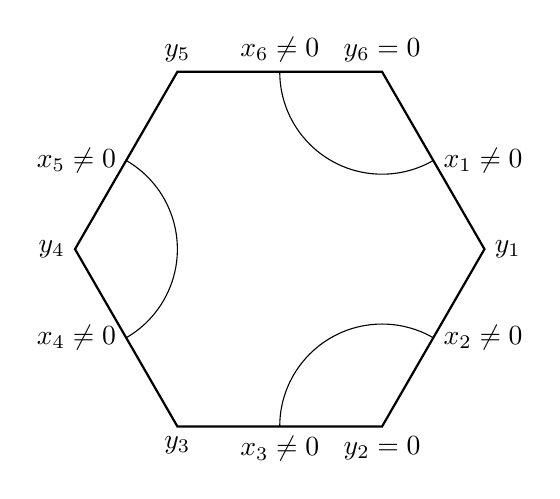
\begin{tikzpicture}[>=angle 90,scale=2.6]
\draw[thick]
(0,0) node[above]{$y_5$}
-- ++(0:0.5) node[above]{$x_6\ne0$}
--  ++(0:0.5) node[above]{$y_6=0$}
--  ++(-60:0.5) node[above,right]{$x_1\ne0$} 
--  ++(-60:0.5) node[right]{$y_1$} 
--  ++(-120:0.5) node[below,right]{$x_2\ne0$}
--  ++(-120:0.5) node[below]{$y_2=0$}
--  ++(180:0.5) node[below]{$x_3\ne0$}
--  ++(180:0.5) node[below]{$y_3$}
-- ++(-240:0.5) node[below,left]{$x_4\ne0$}
-- ++(-240:0.5) node[left]{$y_4$}
-- ++(60:0.5) node[above,left]{$x_5\ne0$}
--cycle;
\draw
(0.5,0) arc (180:300:0.5);
\draw
(0.5,-1.732) arc (180:60:0.5);
\draw
(-0.25,-1.732/4) arc (60:-60:0.5);
\end{tikzpicture}
\end{figure}

%\medskip
%DIAGRAM10
%\sh{-20}{\box\boxJ}
%\medskip

\noindent
$x_{2}+x_{3} = 0; x_{1}+x_{6} = 0$ (so also $x_{4}+x_{5} = 0$).
 Now
$$
{\e}_{\alpha}(x_{1}){\e}_{\beta}(y_{1})\ldots
{\e}_{\alpha}(x_{6}){\e}_{\beta}(y_6) =
{\e}_{\alpha}(x_{5}){\e}_{\beta}(y_{5}+y_{1}+y_{3})
{\e}_{\alpha}(x_{4}){\e}_{\beta}(y_{4}) = 0 .
$$
By (1.3.b), using $x_{4},x_{5}\ne 0$ we have $y_{4} = y_{5}+y_{1}+y_{3} = 0$.
 This is pattern $(G.I)$.
 (We allow the possibility that $y_{1}y_{3}y_{5} = 0$).
\end{proof}

{\medskip}

The following lemma completes the proof of proposition 1.1.

\begin{lemma}{Lemma 3.8}\  $(G_{2})$\  Suppose that $E$ gives the pattern $G.I$.
 Select $W_{+}$ so that ${\theta}_{1}(W_{+},{\beta}) = 0,$\ ${\theta}_{1}(W_{+},
{\alpha})\ne 0,$\ ${\theta}_{1}(W({\sigma}_{\beta}),{\alpha})\ne 0,$
${\theta}_{1}(W({\sigma}_{\beta}{\sigma}_{\alpha}),{\alpha})\ne 0,$
${\theta}_{1}(W({\sigma}_{\alpha}),{\beta})\ne 0,$
${\theta}_{1}(W({\sigma}_{\alpha}{\sigma}_{\beta}),{\beta})\ne 0$ on $E$.
 Then
\begin{enumerate}
\item{a)}\   $z(W_{+},{\alpha})/z(W({\sigma}_{\beta}),{\alpha}) = 1$ on $E$,
\item{b)}\   $z({\beta})$ vanishes on $E$,
\item{c)}\   $n_{{\g}}/(n_{\alpha}n_{\beta}) = -1,
n_{{\delta}}/(n_{\alpha}^{2}n_{\beta}) = -3,
n_{{\e}}/(n_{\alpha}^{3}n_{\beta}) =-5,$
$n_{{\z}}/(n_{\alpha}^{3}n_{\beta}^{2}) = 13$ on $E$;
\item{d)}\   $w({\eta})$ is regular on $E$, ${\eta} = {\g},{\delta},{\e},
{\z}$;
\item{e)}\   $w({\z})$ is invertible on $E$.
\item{f)}\   $E$ is not a subregular divisor.
\end{enumerate}
\end{lemma}

\medskip

\begin{proof} \   Notice that by the equations holding for the pattern $G.I$ we
have $z_{1}(W({\sigma}_{\beta}),{\alpha}) = z_{1}(W_{+},{\alpha})$.
 The minus sign has disappeared because the walls $(W({\sigma}_{\beta}),
{\alpha})$ and $(W_{+},{\alpha})$ have opposite orientations.
 Thus (a) and (b) follow easily.  Now use lemma II.7.3,

\noindent
$m_{\alpha} = 1/z(W_{+},{\alpha})$

\noindent
$m_{\beta} = 1/z(W_{+},{\beta})$

\noindent
$m_{{\g}}/(m_{\alpha}m_{\beta}) = +z(W_{+},
{\alpha})/z(W({\sigma}_{\beta}{\sigma}_{\alpha}),{\alpha}) = -1$ on $E$.

$$\aligned
m_{{\delta}}/(m_{\alpha}^{2}m_{\beta}) =& \\
&\ (z(W_{+},{\alpha})z(W_{+},{\beta}))/(z(W({\sigma}_{\beta}{\sigma}_{\alpha}),
{\alpha})z(W({\sigma}_{\alpha}),{\beta})) \\
&\quad\quad  +
z(W_{+},{\beta})/z(W({\sigma}_{\alpha}),{\beta}) = 0
\endaligned $$ on $E$.

\noindent
$m_{{\e}}/(m_{\alpha}^{3}m_{\beta}) =
-z(W_{+},{\beta})/z(W({\sigma}_{\alpha}),{\beta}) = 0$ on $E$.

\noindent
$m_{{\z}}/(m_{\alpha}^{3}m_{\beta}^{2}) =
-(z(W_{+},{\beta})z(W_{+},{\alpha})^{3})/(z(W({\sigma}_{\alpha}
{\sigma}_{\beta}),{\beta})z(W({\sigma}_{\beta}),{\alpha})^{3}) - $
$$
z(W_{+},{\alpha})^{3}/z(W({\sigma}_{\beta}),{\alpha})^{3} = -1\
{\text{on}}\  E	.
$$
Now apply (II.7.2).  Recall that $a = b = c = d = 1, e = 2, f = g = h = j = 3,$
$i=-1.$

\noindent
$-1 =   m_{{\g}}/(m_{\alpha}m_{\beta}) =
n_{{\g}}/(n_{\alpha}n_{\beta})$ on $E$

\noindent
$0 = m_{{\delta}}/(m_{\alpha}^{2}m_{\beta}) =
n_{{\delta}}/(n_{\alpha}^{2}n_{\beta}) +
b -en_{{\g}}/(n_{\alpha}n_{\beta}) =
n_{{\delta}}/(n_{\alpha}^{2}n_{\beta}) + b + e$;

   $n_{{\delta}}/(n_{\alpha}^{2}n_{\beta}) = -b -e = -3$.

\noindent
$0 = m_{{\e}}/(m_{\alpha}^{3}m_{\beta}) =
n_{{\e}}/(n_{\alpha}^{3}n_{\beta}) - c +
fn_{{\g}}/(n_{\alpha}n_{\beta}) - hn_{{\delta}}/(n_{\alpha}^{2}
n_{\beta}) =$

$n_{{\e}}/(n_{\alpha}^{3}n_{\beta}) -1 + 3(-1) - 3(-3)$;

$n_{{\e}}/(n_{\alpha}^{3}n_{\beta}) = -5.$

\medskip

\noindent
$-1 =   m_{{\z}}/(m_{\alpha}^{3}m_{\beta}^{2}) =
n_{{\z}}/(n_{\alpha}^{3}n_{\beta}^{2}) -
in_{{\e}}/(n_{\alpha}^{3}n_{\beta})$

-$j(n_{{\g}}/(n_{\alpha}n_{\beta}))
(n_{{\delta}}/(n_{\alpha}^{2}n_{\beta}) =
n_{{\z}}/(n_{\alpha}^{3}n_{\beta}^{2}) + 1(-5) -3(3)$;

$n_{{\z}}/(n_{\alpha}^{3}n_{\beta}^{2}) = -1+5+9 = 13$.

\medskip

\noindent
Parts (c) and (d) now follow immediately.
 Write $(1-{\alpha}^{-1})/{\lambda} \vert_{E} = A,
(1-{\beta}^{-1})/{\lambda} \vert_{E} = B$, etc.
 By lemma 2.2,

\medskip

$$
\aligned
w({\z}) &=  Z(n_{{\z}}/n_{\alpha}^{3}n_{\beta}) +
gA(n_{{\g}}/(n_{\alpha}n_{\beta}))^{2} -
iB(n_{{\e}}/n_{\alpha}^{3}n_{\beta}) - \\
&\quad j{\Gamma}(n_{{\g}}/n_{\alpha}n_{\beta})(n_{{\delta}}/n_{\alpha}^{2}
n_{\beta}) - ejA(n_{{\g}}/n_{\alpha}n_{\beta})^{2} +
ajA(n_{{\delta}}/n_{\alpha}^{2}n_{\beta}) = \\
&= Z(13) + gA -iB(-5) -j{\Gamma}(-1)(-3) -ejA +ajA(-3) \\
&= 13Z + 3A -5B -9{\Gamma} -6A -9A \\
&= 13Z -21A -14B = 6Z \ne 0
\endaligned
$$
because the tangent of our curve lies in no singular hyperplanes.
This proves (e).
\end{proof}

\medpagebreak

\noindent
$w({\z})x({\eta}) = w({\eta})x({\z})z({\alpha})^{m({\alpha})}
z({\beta})^{m({\beta})}$ where ${\z}-{\eta} =
m({\alpha}){\alpha}+m({\beta}){\beta}$.
 If ${\eta}\ne {\z}, x({\eta}) = 0$ on $E$ because $w({\z})$ is
invertible, $m({\beta}) > 0$, and $z({\beta})$ vanishes on $E$.
 Thus $E$ is certainly not a subregular divisor.

%% end of cthis.tex

%% start of dthis.tex


\chapter{The Subregular Spurious Divisor}




\section{Subregular\ Unipotent\ Conjugacy\ Classes}


   This section reviews well known results on the subregular conjugacy
class of a reductive group.  For details see \cite{MR0352279}.  Let $G$ be a
reductive group.  $A$ subregular unipotent conjugacy class of $G$ is a
conjugacy class whose centralizer has dimension $rank(G)+2$.  Conjugacy
classes are taken over the algebraic closure of the base field unless
specifically stated otherwise.  Simple algebraic groups possess exactly one
subregular unipotent conjugacy class.  More generally a reductive group
contains as many subregular unipotent conjugacy classes as there are
connected components of the Dynkin diagram.  Each subregular unipotent
element determines a connected component of the Dynkin diagram.  The
variety of Borel subgroups containing a subregular unipotent element $u$,
$(B\backslash G)_{u}$, is a union of projective lines and is called a Dynkin
curve.  Let $P_{{\alpha}}$ denote the parabolic subgroup associated with
the simple root ${\alpha}$.  Each line is of the form $B\backslash
P_{{\alpha}}g$ for some $g \in G$.  The root ${\alpha}$ is uniquely
determined by the line, and the line is said to be of type ${\alpha}$.  $A$
line of type ${\alpha}$ does not intersect a line of type ${\beta}$ if
$({\alpha},{\beta})=0$.  The number of lines in $(B\backslash G)_{u}$ and
their incidence relations depends only on the connected component of the
Dynkin diagram determined by $u$.  There is always one line for each of the
shorter roots, and two lines for each of the longer roots except for
$G_{2}$ where there are three lines corresponding to the long root.
There are $\langle{-\beta},{\alpha}\rangle$ lines of type ${\beta}$ intersecting
each line of type
${\alpha}$.

%XXD
\begin{figure}[htb]
\centering
\begin{tikzpicture}[>=angle 90,scale=1]
\node[text width=3cm,align=justify] at (0,0.35) {
Examples of\par 
Dynkin Curves
};

%G2-D4
\node[text width=3cm,align=justify,xshift=0cm,yshift=-2cm] at (0,0) {
$G_2$, $D_4$
};
% bottom part
\draw[xshift=0cm,yshift=-0.5cm,scale=0.8]
(1,-0.8)--(1,-2.2);
\draw[xshift=0cm,yshift=-0.5cm,scale=0.8]
(0.8,-2)--(2.2,-2);
\draw[xshift=0cm,yshift=-0.5cm,scale=0.8]
(2,-2.2)--(2,-0.8);
%\draw[xshift=0cm,yshift=-0.5cm,scale=0.8]
%(1.8,-1)--(3.2,-1);
\draw[xshift=0cm,yshift=-0.5cm,scale=0.8]
(1.5,-1.5)--(1.5,-2.5);
\draw[xshift=0cm,yshift=-0.5cm,scale=0.8]
(1.5,-2) circle (0.12);

%F4-E6
\node[text width=3cm,align=justify,xshift=0cm,yshift=-4cm] at (0,0) {
$F_4$, $E_6$
};
% bottom part
\draw[xshift=0cm,yshift=-2.5cm,scale=0.8]
(-0.2,-1)--(1.2,-1);
\draw[xshift=0cm,yshift=-2.5cm,scale=0.8]
(1,-0.8)--(1,-2.2);
\draw[xshift=0cm,yshift=-2.5cm,scale=0.8]
(0.8,-2)--(2.2,-2);
\draw[xshift=0cm,yshift=-2.5cm,scale=0.8]
(2,-2.2)--(2,-0.8);
\draw[xshift=0cm,yshift=-2.5cm,scale=0.8]
(1.8,-1)--(3.2,-1);
\draw[xshift=0cm,yshift=-2.5cm,scale=0.8]
(1.5,-1.5)--(1.5,-2.5);
\draw[xshift=0cm,yshift=-2.5cm,scale=0.8]
(1.5,-2) circle (0.12);


%BnAn
\node[text width=3cm,align=justify,xshift=0cm,yshift=-5.5cm] at (0,0) {
$B_n$, $A_{2n+1}$
};
\draw[xshift=0cm,yshift=-6cm,scale=0.8]
(-0.2,0)--(1.2,0);
\draw[xshift=0cm,yshift=-6cm,scale=0.8]
(1,-0.2)--(1,1.2);
\draw[xshift=0cm,yshift=-6cm,scale=0.8]
(0.8,1)--(2.2,1);
\draw[xshift=0cm,yshift=-6cm,scale=0.8]
(2,1.2)--(2,-0.2);
\draw[xshift=0cm,yshift=-6cm,scale=0.8]
(1.8,0)--(3.2,0);
% bottom part
\draw[xshift=0cm,yshift=-6cm,scale=0.8]
(0,0.2)--(0,-1.2);
\draw[xshift=0cm,yshift=-6cm,scale=0.8]
(-0.2,-1)--(1.2,-1);
\draw[xshift=0cm,yshift=-6cm,scale=0.8]
(1,-0.8)--(1,-2.2);
\draw[xshift=0cm,yshift=-6cm,scale=0.8]
(0.8,-2)--(2.2,-2);
\draw[xshift=0cm,yshift=-6cm,scale=0.8]
(2,-2.2)--(2,-0.8);
\draw[xshift=0cm,yshift=-6cm,scale=0.8]
(1.8,-1)--(3.2,-1);

%E8
\node[text width=3cm,align=justify,xshift=8.5cm,yshift=-5.2cm] at (0,0) {
$E_8$
};
\draw[xshift=7.8cm,yshift=-6cm,scale=0.8]
(-0.2,0)--(1.2,0);
% bottom part
\draw[xshift=7.8cm,yshift=-6cm,scale=0.8]
(0,0.2)--(0,-1.2);
\draw[xshift=7.8cm,yshift=-6cm,scale=0.8]
(-0.2,-1)--(1.2,-1);
\draw[xshift=7.8cm,yshift=-6cm,scale=0.8]
(1,-0.8)--(1,-2.2);
\draw[xshift=7.8cm,yshift=-6cm,scale=0.8]
(0.8,-2)--(2.2,-2);
\draw[xshift=7.8cm,yshift=-6cm,scale=0.8]
(2,-2.2)--(2,-0.8);
\draw[xshift=7.8cm,yshift=-6cm,scale=0.8]
(1.8,-1)--(3.2,-1);
\draw[xshift=7.8cm,yshift=-6cm,scale=0.8]
(1.5,-1.5)--(1.5,-2.5);
\draw[xshift=7.8cm,yshift=-6cm,scale=0.8]
(1.5,-2) circle (0.12);

%E7
\node[text width=3cm,align=justify,xshift=5cm,yshift=-5.2cm] at (0,0) {
$E_7$
};
% bottom part
\draw[xshift=4.3cm,yshift=-6cm,scale=0.8]
(0,0.2)--(0,-1.2);
\draw[xshift=4.3cm,yshift=-6cm,scale=0.8]
(-0.2,-1)--(1.2,-1);
\draw[xshift=4.3cm,yshift=-6cm,scale=0.8]
(1,-0.8)--(1,-2.2);
\draw[xshift=4.3cm,yshift=-6cm,scale=0.8]
(0.8,-2)--(2.2,-2);
\draw[xshift=4.3cm,yshift=-6cm,scale=0.8]
(2,-2.2)--(2,-0.8);
\draw[xshift=4.3cm,yshift=-6cm,scale=0.8]
(1.8,-1)--(3.2,-1);
\draw[xshift=4.3cm,yshift=-6cm,scale=0.8]
(1.5,-1.5)--(1.5,-2.5);
\draw[xshift=4.3cm,yshift=-6cm,scale=0.8]
(1.5,-2) circle (0.12);

%Cn-Dn
\node[text width=3cm,align=justify,xshift=5cm,yshift=1cm] at (0,0) {
$C_n$, $D_{n+1}$
};
\begin{scope}
\foreach\x in {1,3,5,6,7}
\draw[xshift=1.8cm,yshift=-0.2cm,scale=0.56]
(3+\x -0.2, -0.2)--(3+\x+1.2,1.2);
\foreach\x in {2,4,6}
\draw[xshift=1.8cm,yshift=-0.2cm,scale=0.56]
(3+\x -0.2, 1.2)--(3+\x+1.2,-0.2);
\draw[xshift=1.8cm,yshift=-0.2cm,scale=0.56]
(3+2,1.0) circle (0.2);
\end{scope}

%A2n
\node[text width=3cm,align=justify,xshift=5cm,yshift=-1cm] at (0,0) {
$A_{2n}$
};
\begin{scope}
\foreach\x in {1,3,5}
\draw[xshift=1.8cm,yshift=-2.2cm,scale=0.56]
(3+\x -0.2, -0.2)--(3+\x+1.2,1.2);
\foreach\x in {2,4,6}
\draw[xshift=1.8cm,yshift=-2.2cm,scale=0.56]
(3+\x -0.2, -3.2)--(3+\x+1.2,-1.8);


% downstrokes
\foreach\x in {2,4,6}
\draw[xshift=1.8cm,yshift=-2.2cm,scale=0.56]
(3+\x -0.2, 1.2)--(3+\x+1.2,-0.2);

\foreach\x in {1,3,5}
\draw[xshift=1.8cm,yshift=-2.2cm,scale=0.56]
(3+\x -0.2, -1.8)--(3+\x+1.2,-3.2);

% front strokes
\draw[xshift=1.8cm,yshift=-2.2cm,scale=0.56]
(3+1 -0.2, -2.2)--(3+1+1.2,-0.8);
\draw[xshift=1.8cm,yshift=-2.2cm,scale=0.56]
(3+1 -0.2, 0.2)--(3+1+1.2,-1.2);
\draw[xshift=1.8cm,yshift=-2.2cm,scale=0.56]
(3+2,-1.0) circle (0.2);
%\draw[xshift=1.8cm,yshift=-2.2cm]
%(3+6+0.5,0.5) circle (0.12);
\end{scope}


\end{tikzpicture}
\end{figure}

%\vfill\eject
%\medskip
%DIAGRAM11
%\hrule\medskip\box\boxK\medskip\hrule
%\medskip

   The line $B\backslash P_{{\alpha}}g$ is a line in $(B\backslash G)_{u}$
if and only if $u^{g^{-1}}$ is contained in the unipotent radical of
$P_{{\alpha}}$.  For a point $p \in Y_{{\Gamma}}$ such that ${\pi}(p) = u$
is subregular unipotent, let $L_{p}(W)$ be the set of simple roots ${\alpha}$ such
that $B(W)$ lies in a line of type ${\alpha}$ in $(B\backslash G)_{u}$.
From the fact that no Borel subgroup lies in more than two lines of
$(B\backslash G)_{u}$ it follows that $\vert L_{p}(W)\vert = 1$ or $2$.  Also
if ${\alpha}, {\beta} \in L_{p}(W)$ then $({\alpha},{\beta})\ne 0$
because a line of type ${\alpha}$ does not intersect any lines of type
${\beta}$ when $({\alpha},{\beta}) = 0$.  Consider a coordinate patch
$S(B_{{\infty}},B_{0})$.


Recall $x(W,{\alpha})$ is defined to be $x({\alpha})(u^{n_w^{-1}})$.

\begin{lemma}{Lemma 1.1} ${\alpha} \in L_{p}(W)$ if and only if
$x(W,{\alpha}) = 0$ at $p$.
\end{lemma}

\medpagebreak

\begin{proof}  $0 = x(W,{\alpha})$ if and only if $u^{\nu^{-1}n_w^{-1}}$
lies in the unipotent radical of $P_{{\alpha}}$
the parabolic subgroup of type ${\alpha}$ containing the Borel $B_{0}$.  So
the line $B_{0}\backslash P_{{\alpha}}n_{w}{\nu}$ containing $B_{0}^{n_w\nu}$
lies in the Dynkin curve and conversely.
\end{proof}

{\medskip}

   Note also that $L_{p}(W) = L_{p}(W')$ if $z(W,{\alpha}) = 0$ and that
$z(W,{\alpha}) = 0$ if $B(W) = B(W')$ where $(W,{\alpha})$ is the wall
separating adjacent chambers $W$ and $W'$.  For every simple root
${\alpha}$, we fix a wall $(W_{{\alpha}},{\alpha})$ of type ${\alpha}$ such
that ${\theta}_{1}(W_{{\alpha}},{\alpha})\ne 0$, and set
$$
\tilde{z} (W,{\alpha}) = z(W,{\alpha})/z(W_{{\alpha}},{\alpha}) =
z_{1}(W,{\alpha})/z_{1}(W_{{\alpha}},{\alpha})
$$
By the definitions of $\tilde z (W,{\alpha})$ and ${\theta}_{1} (III.1)$ we
have $\tilde z (W,{\alpha}) = 0$ if and only if ${\theta}_{1}(W,{\alpha}) =
0$.  By abuse of language we will often say that the wall $(W,{\alpha})$ is
non-zero if ${\theta}_{1}(W,{\alpha})\ne 0$.  The following equations hold
on $Y_{1}(B_{{\infty}},B_{0})$ for any two Weyl chambers $W$ and $W'$ where
$T(W,{\alpha}) = (1-{\gamma}^{-1})/{\lambda}$ and ${\pm}{\gamma}$ is
the root such that ${\gamma} = 0$ defines the wall $(W,{\alpha})$.


\begin{eqn}  %{Equation\ 1.2}
$$
\lambda T(W,{\alpha}) = z({\alpha})z_{1}(W,{\alpha})x(W,{\alpha}) =
z(W,{\alpha})x(W,{\alpha})
$$
\end{eqn}

$$
\tilde {z} (W,{\alpha})x(W,{\alpha})T(W',{\alpha}) = T(W,{\alpha})\tilde z
(W',{\alpha})x(W',{\alpha}) .
$$
$T(W,{\alpha})$ is regular and invertible at ${\lambda} = 0$.  Also it
follows immediately from (1.1) and this equation that if
$z(W,{\alpha})\ne 0$ then ${\alpha} \in L_{p}(W)$.

\medskip

\begin{corollary}{Corollary 1.3}\ For any given Weyl chamber $W$ and $p$ with
${\pi}(p) = u$, $u \in G(\Fb)$ subregular there are at most two simple
roots ${\alpha}$ such that $z(W,{\alpha})\ne 0$.  If $z(W,{\alpha})\ne 0$
then ${\alpha} \in L_{p}(W)$.
\end{corollary}

\medskip

\begin{proof} \  No point of $(B\backslash G)_{u}$ lies in more than
two lines.
\end{proof}


\section{{Exclusion\ of\ Spurious\ Divisors}}

\begin{theorem}{Theorem 2.1}    Let $E$ be a subregular spurious divisor.
 Then ${\beta}(E) > 2$.
\end{theorem}

\medpagebreak

\begin{proof} \ Select a wall $(W,{\alpha})$ such that
${\theta}_{1}(W,{\alpha}) = 0$.  Select a wall $(W',{\alpha})$ such that
${\theta}_{1}(W',{\alpha})\ne 0$.  Form a path $W' = W_{0},W_{1},\ldots ,
W_{p} = W$ from $W'$ to $W$.  Suppose that $W_{i}$ and $W_{i+1}$ are
separated by a wall of type ${\alpha}_{i}, i = 0,\ldots ,p-1$.  Corresponding
to this path is a sequence of walls $(W_{i},{\alpha})\  i = 0,1,\ldots ,p$.
Let $j$ be the smallest index for which ${\theta}_{1}(W_{j},{\alpha}) = 0$.
Since ${\theta}_{1}(W,{\alpha}) = 0$ such an index exists.  Since
${\theta}_{1}(W',{\alpha})\ne 0, j > 0$.  Then
${\theta}_{1}(W_{j},{\alpha}) = 0$ and ${\theta}_{1}(W_{j-1},{\alpha})\ne 0$.
The simple root ${\alpha}_{j-1}$ cannot equal ${\alpha}$.  By the nature of
the equations holding at a node of type $A_{1} \times A_{1}$ (III.1) we see
that $({\alpha}_{j-1},{\alpha})\ne 0$.

   Suppose first of all that ${\alpha}$ can be chosen so that
   $|\alpha_{j-1}|\ge |\alpha|$.
  The hypotheses
of (III.3.1) now hold so that we can exclude the divisor.

   Now assume that no matter how ${\alpha}$ is chosen $|\alpha_{j-1}|< |\alpha|$.
  It follows that if ${\beta}$
is adjacent to ${\alpha}$ then ${\theta}_{1}(W,{\beta})\ne 0$ for all $W$.
Thus at the node defined by the two walls $(W_{j-1},{\alpha}_{j-1})$ and
$(W_{j-1},{\alpha})$ none of the walls of type ${\alpha}_{j-1}$ are zero
and ${\theta}_{1}(W_{j-1},{\alpha}) = 0, {\theta}_{1}(W_{j},{\alpha})\ne 0$.
This by definition is a special node.  Proposition III.1.1 now shows that
${\beta}(E) > 2$.
\end{proof}

\section{The\ graph\ $\Gamma_0$}

The remainder of this chapter discusses the structure of subregular spurious
divisors and their zero patterns.  These structural results will not be
used in any of the following chapters.  We assume that $G = A_{n}, B_{n},
C_{n}$ or $D_{n+1}, n \ge  3$ over an algebraically closed field $\Fb$.
We fix a point $p$ in a divisor such that ${\pi}(p) \in G(\Fb)$ is
subregular unipotent.  Let $R$ be the set of roots ${\alpha}$ such that
$z(W,{\alpha})\ne 0$ for some $W$.  Let $S$ be the set of roots ${\alpha}$
such that ${\theta}_{1}(W,{\alpha}) = 0$ for some $W$.  Define a {\it solid
node} to be a node at which ${\theta}_{1}(W,{\alpha})\ne 0$ for all walls
$(W,{\alpha})$ at the node.  We make the following assumption which remains
in effect until section $8$.


\begin{assumption}  %{Assumption\ 3.1}
$\vert S\vert \ge 2$ and if ${\alpha},
{\beta} \in S$ then there are no solid nodes of type
$({\alpha},{\beta})$.
\end{assumption}

   We will see in section $8$, that this assumption holds except in a few
exceptional easily categorized cases.

\medpagebreak

\begin{lemma}{Lemma 3.2}  $S {\supseteq} R$.
\end{lemma}

\medpagebreak

\begin{proof} \ Suppose ${\alpha} \in R\backslash S$.  We will show
that $\vert S\vert \le 1$, contrary to assumption 3.1.  If ${\alpha}
\in R\backslash S$, then $z(W,{\alpha})\ne 0$ for all $W$.  Thus by
$(1.2), x(W,{\alpha}) = 0$ for all $W$.  Let ${\beta}  \in  S$.  Then again
by $(1.2)$, $\tilde z (W,{\beta})x(W,{\beta}) = 0$ for all ${\beta}$ (since
$\tilde z (W,{\beta}) = 0$ for some W).  Pick $W = W'$ such that
${\theta}_{1}(W',{\beta})\ne 0$.  Then $x(W',{\alpha})$ $= x(W',{\beta}) =
0$.  Since ${\pi}(p)$ is assumed to be subregular, ${\alpha}$ and ${\beta}$
are adjacent.

   Assume that ${\alpha}$ and ${\beta}$ are the same length.  Then the fact
that ${\theta}_{1}(W,{\alpha})\ne 0$ for all $(W,{\alpha})$ together with
the fact that ${\theta}_{1}(W',{\beta})\ne 0$ forces the node of type
$A_{2}$ formed by the walls $(W',{\alpha})$ and $(W',{\beta})$ to be a
solid node.  (See the list of zero patterns for a node of type $A_{2}.)$
Thus $$x(W,{\alpha}) = x(W,{\beta}) = 0$$ for all walls $(W,{\alpha})$,
$(W,{\beta})$ at the node.  This shows that ${\alpha}, {\beta}  \in
L_{p}(W)$ for all Weyl chambers $W$ at the node.  There is exactly one
Borel subgroup $B_{+}$ which lies at the intersection of a line of type
${\alpha}$ with a line of type ${\beta}$.  Thus $B(W) = B_{+}$ for all $W$
at the node.  This contradicts the fact that $z(W',{\alpha})\ne 0$
$(B(W')\ne
B(W'')$ where $W''$ is the chamber through a wall of type ${\alpha}$ from
$W')$.  We conclude that ${\alpha}$ and ${\beta}$ have different lengths.

   For a reductive group the assumption that $S$ is a set such that if
${\beta}  \in  S$ then $({\beta},{\alpha})\ne 0$ and ${\alpha}$ and
${\beta}$ are different lengths forces $\vert S\vert \le 1$.  This
proves the lemma.
\end{proof}

{\medskip}


   We form an equivalence relation on the non-zero walls $(W,{\alpha})$ of
type ${\alpha}$ for ${\alpha}  \in  S$.  Say that two non-zero walls
$(W,{\alpha})$ and $(W',{\alpha})$ are equivalent if $(I)$ there is a path
$W = W_{0},\ldots ,W_{p} = W'$ from $W$ to $W'$ such that if
${\theta}_{1}(W_{i},{\alpha}_{i})\ne 0$ then ${\alpha}_{i} {\notin} S$ or
if $(II) \ (W,{\alpha})$ and $(W',{\alpha})$ are the two non-zero colinear
walls at a node of type $B_{2}$ with zero pattern $B.III$ or $B.IV$:
\medskip
%DIAGRAM12
\sh{-12}{\box\boxL}
\medskip

\noindent
The equivalence classes are defined to be the smallest classes such that
(I) and (II) are satisfied.

   Form a graph ${\Gamma}_{0}$ as follows.  Let each vertex be given by an
equivalence class of walls.  $A$ vertex $v_{1}$ of ${\Gamma}_{0}$ is said
to be of type ${\alpha} \ (type(v_{1})={\alpha})$ if the walls of the
equivalence class are of type ${\alpha}$.  Join two vertices $(v_{1}\ne
v_{2})$ by an edge if there is a series of chambers $W_{0},\ldots ,W_{p}$
separated by walls $(W_{i},{\alpha}_{i}) \ i = 0,\ldots ,p-1$ such that
$(W_{0},type(v_{1}))$ is a wall of $v_{1}, (W_{p},type(v_{2}))$ is a wall
of $v_{2}$, and if ${\theta}_{1}(W_{i},{\alpha}_{i})\ne 0$ then
${\alpha}_{i} {\notin} S$ for $i = 0,\ldots ,p-1$.

\medskip

\begin{lemma}{Lemma 3.3} If the vertices $v_{1}$ and $v_{2}$ are joined
then $$(type(v_{1}),type(v_{2}))\ne 0.$$
\end{lemma}

\medpagebreak

\begin{proof} \ By construction a vertex is not joined to itself by an
edge.
\end{proof}

\medpagebreak

   We use equation 1.2 in the form
$$
\tilde {z} (W,{\alpha})x(W,{\alpha})T(W',{\alpha}) = T(W,{\alpha})\tilde z
(W',{\alpha})x(W',{\alpha}).
$$
Since $type(v_{1})  \in  S$, there is a $W'$ such that
${\theta}_{1}(W',type(v_{1}))=0$.  It follows that $\tilde z(W,{\alpha})x(W,{\alpha})=0$
for all $W$ where ${\alpha} = type(v_{1})$.  If
$(W,{\alpha})  \in  v_{1}$ then ${\theta}_{1}(W,{\alpha})\ne 0$ and
$x(W,{\alpha}) = 0$ so that ${\alpha}  \in  L_{p}(W)$.  Similarly, if
$$(W',type(v_{2}))  \in  v_{2} \quad \hbox{then}\quad  type(v_{2})  \in  L_{p}(W').$$
Selecting a path between appropriately selected chambers $W$ and $W'$, we
see that the intervening walls are zero $(z(W_{i},{\alpha}_{i}) = 0) (3.2)$
so that $B(W) = B(W')$ and $L_{p}(W) = L_{p}(W')$.  So $$type(v_{1}),\
type(v_{2})  \in  L_{p}(W).$$  $B(W)$ lies in lines of type $type(v_{1})$
and $type(v_{2})$.  By the nature of the Dynkin curve
$(type(v_{1}),type(v_{2})) \ne 0$.

{\medskip}

   Every path $W_{0},\ldots ,W_{p}$ through the Weyl chambers gives rise to
a path through the graph ${\Gamma}_{0}$ as follows.  Let $W_{a_1},\ldots ,
W_{a_j} \ a_{1} < a_{2} < \ldots < a_{j}$ be the indices of
the chambers in the path such that ${\theta}_{1}(W_{a_{i}},{\alpha}_{a_{i}})
\ne 0$ and ${\alpha}_{a_{i}}  \in  S$.  Then
let $v_{i}$ be the vertex corresponding to the wall $(W_{a_{i}},
{\alpha}_{a_{i}})$.  By construction $v_{i}$ is joined by an edge
to $v_{i+1}$ provided $v_{i}\ne v_{i+1}$.  It is clear that if the path
through the Weyl chambers is taken to be closed $W_{0},\ldots ,
W_{p},W_{p+1} = W_{0}$ then the corresponding path through the graph
${\Gamma}_{0}$ will be closed.  Since we can always select a path
$W_{0},\ldots ,W_{p}$ between any two given walls $(W,{\alpha})$ and
$(W',{\beta})$, there is a path in ${\Gamma}_{0}$ between any two given
vertices.  Thus ${\Gamma}_{0}$ must be a connected graph.  This proves part
(a) of the following lemma.

\medskip

\begin{lemma}{Lemma 3.4}
\begin{enumerate}[label=\alph*)]
\item The graph ${\Gamma}_{0}$ is connected.
\item ${\Gamma}_{0}$ is a tree.
\item $S$ forms a connected Dynkin diagram.
\end{enumerate}
\end{lemma}

\medskip


\begin{proof}  (a) has been proved and (c) follows directly from
(a) and (3.3).

   (b)\ We have described a map from closed paths $W_{0},\ldots
,W_{p},W_{p+1} = W_{0}$ through the Weyl chambers to the closed paths in
${\Gamma}_{0}$.  (b) will follow from two facts.  First, a homotopy of
paths in the Weyl chambers maps to a homotopy of paths in ${\Gamma}_{0}$.
Second, every closed path in ${\Gamma}_{0}$ is homotopic to the image of a
closed path through the Weyl chambers.  If we have these two facts then
(b) follows from the fact that any closed path through the Weyl chambers
is contractable.  We do not require that the homotopies fix a base point.

   To check that a homotopy of paths in the Weyl chambers maps to a
homotopy of paths in ${\Gamma}_{0}$, it is enough to check the statement as
the homotopy passes through a wall or node.  We begin with a special case.
Suppose that part of the path $L$ is
$$
\ldots W_{i},W_{i+1},\ldots ,W_{i+k}=W_{i},W_{i+k+1},\ldots
$$
which a homotopy carries to
$$
L':  \ldots W_{i},W_{i+k+1},\ldots
$$
Suppose that there is a vertex $v$ of ${\Gamma}_{0}$ such that for all $j$
in the range $i \le j < i+k$ we have: If
${\theta}_{1}(W_{j},{\alpha}_{j})\ne 0$ and ${\alpha}_{j}  \in  S$ then
$(W_{j},{\alpha}_{j})$ belongs to the vertex $v$ of ${\Gamma}_{0}$.  Let
$(W_{\ell},{\alpha}_{{\ell}})$ be the wall with the largest index
${\ell}$ such that ${\ell} < i, {\alpha}_{{\ell}}  \in  S$ and
${\theta}_{1}(W_{{\ell}},{\alpha}_{{\ell}}) \ne 0$.  Let $v_{a}$ be the
vertex of ${\Gamma}_{0}$ corresponding to $(W_{{\ell}},{\alpha}_{{\ell}})$.
If $v \ne v_{{\alpha}}, v$ and $v_{{\alpha}}$ are joined by an edge.
Similarly let $(W_{{\ell}'},{\alpha}_{{\ell}'})$ be the wall with the
smallest index ${\ell}'$ such that ${\ell}' \ge i+k, {\alpha}_{{\ell}'}
 \in  S$ and ${\theta}_{1}(W_{{\ell}'},{\alpha}_{{\ell}'}) \ne 0$.  Let
$v_{b}$ be the vertex of ${\Gamma}_{0}$ corresponding to
$(W_{{\ell}'},{\alpha}_{{\ell}'})$.  If $v \ne v_{b}$ then $v$ and $v_{b}$
are joined by an edge.


   I claim that $v_{a}, v_{b}$, and $v$ are not distinct vertices.  For if
they were distinct, there would be edges between each pair, and their types
(a simple root in $S$) would be distinct.  This by (3.3), would give a
closed loop in the Dynkin diagram of $G$.

   If $v = v_{a}$ or $v_{b}$ then paths $L$ and $L'$ give rise to the same
path in ${\Gamma}_{0}$.  If $v_{a} = v_{b}$, then the paths in
${\Gamma}_{0}$ corresponding to $L$ and $L'$ are given by the following
diagram.

\medskip
%DIAGRAM13
\sh{-15}{\box\boxM}\medskip


\noindent
They are clearly homotopic.

   This special case takes care of the situation where the homotopy moves
through a wall or through a node of type $({\alpha},{\beta})$ such that if
${\beta}  \in  S$ then ${\theta}_{1}(W,{\beta}) = 0$ for all walls
$(W,{\beta})$ at the node.  We must still consider a homotopy that moves
through a node of type $({\alpha},{\beta})$ with ${\alpha},{\beta}  \in
S$.  By assumption  3.1, we may assume that it is a special node.  The
following diagrams now make it clear that the homotopy of paths in the Weyl
chambers translates to a homotopy of ${\Gamma}_{0}$.

\medskip
%DIAGRAM14
\sh{-15}{\box\boxN}\medskip
\hrule\medskip
%DIAGRAM15
\sh{-15}{\box\boxO}\medskip


We turn to the second fact: that every path in ${\Gamma}_{0}$ has the same
homotopy class as the image of a path through the Weyl chambers.  This
would be obvious by the definitions of the vertices and edges of the graph
were it not for condition (II) defining the equivalence relation on walls
belonging to a given vertex.  It is enough to check that if $(W,{\alpha})$
and $(W',{\alpha})$ are the two non-zero colinear walls at a node (with
pattern B.III or B.IV) belonging to the vertex $v$ of ${\Gamma}_{0}$,
then there is a path joining $(W,{\alpha})$ to $(W',{\alpha})$ whose image
in ${\Gamma}_{0}$ is a path homotopic to the constant path at the vertex
$v$.  This is completely evident from the following diagram.

\medskip
%DIAGRAM16
\sh{-15}{\box\boxP}\medskip
\end{proof}

\section{The\ Modified\ Star}

   Let $S_{2}$ be the affine variety generated by the variables $\hat
z({\alpha})$ ${\ \forall\ } {\alpha}$, $\hat z(W,{\alpha})$ ${\ \forall\ }
(W,{\alpha})$ subject to the relations:
\begin{enumerate}[label=\roman*)]
\item $\hat z(W,{\alpha})+\hat z(W'{\alpha}) = 0$ where $W$ and $W'$ are
adjacent walls separated by a wall of type ${\alpha}$, and
\item $\exp(\hat z_{p}X_{-{\alpha}_{p}})\ldots \exp(\hat z_{1}X_{-{\alpha}_{1}})
= 1$ where $W_{1},W_{2},\ldots ,W_{p}$ is the path around
a node (so that $p = 4,6,8$ according as the node is of type $A_{1}xA_{1},
A_{2}, B_{2})$ and $\hat z_{1},\ldots ,\hat z_{p}$ are the corresponding
variables.
\item $\hat z(W_{{\alpha}},{\alpha}) = 1$
for some chamber $W_\alpha$ (unless $\hat z(W,\alpha)=0,\quad \forall W)$.
\end{enumerate}

\noindent
By (I.3.1) there is an injection from the affine patch
$$
\{x  \in  S_{1}(B_{{\infty}},B_0):
{\theta}_{1}(W_{{\alpha}},{\alpha})\ne 0\}
$$
to $S_{2}$ given by $\hat z(W,{\alpha}) {\to} \tilde z (W,{\alpha}), \hat
z({\alpha}) {\to} z(W_{{\alpha}},{\alpha})$.  Elements of $S_{2}$ will be
called {\it  modified stars}.

\medskip

\begin{lemma}{Lemma 4.1} Suppose that all the walls corresponding to a
given vertex of ${\Gamma}_{0}$ are set equal to zero.  Then the resulting
equations define a modified star.
\end{lemma}

\medskip

\begin{proof} \ To check this it is sufficient to verify that the
equations at every node are still satisfied.  But this is immediate from
the definition of a vertex of ${\Gamma}_{0}$.
\end{proof}


\subsection{Modifications}

   We now modify the graph.  Every time a vertex is eliminated from the
graph, we set all corresponding walls to zero in the star.  Doing so gives
a new modified star by (4.1).  The new star will have a graph ${\Gamma}'$
associated to it.  When an extremal vertex of the graph ${\Gamma}_{0}$ is
eliminated, the modified graph ${\Gamma}'$ is a subgraph of ${\Gamma}_{0}$.
  If $G = D_{n}, \vert S\vert \ge 4,
{\alpha}_{+},{\alpha}_{-}  \in  S$ where ${\alpha}_{+}$ and ${\alpha}_{-}$
are simple roots interchanged by an outer automorphism of $G$, then let
$S_{-} = S\backslash \{{\alpha}_{-}\}$.  Otherwise set $S_-=S$.
Thus $S_{-}$ forms a connected
Dynkin diagram with two extremal simple roots.

   Modify the graph as follows.
\begin{enumerate}[label=\arabic*.]
\item For every extremal simple root of the Dynkin diagram $S_{-}$ fix a
vertex of that type in ${\Gamma}_{0}$.
\item Let ${\Gamma}_{1}$ be the minimal tree containing these two vertices.
Eliminate the vertices not in ${\Gamma}_{1}$ and set the corresponding
walls of the star equal to zero.  The resulting star will have graph
${\Gamma}_{1}$.
\item ${\Gamma}_{1}$ is linear.  Let ${\alpha}_{1},\ldots ,{\alpha}_{n}$ be
the roots of $S_{-}$ ordered in such a way that if
$({\alpha}_{i},{\alpha}_{j})\ne 0$ then $\vert i-j\vert \le 1$.  Let
$v_{1}$ (resp.  $v_{n})$ be the extremal vertex in ${\Gamma}_{1}$
corresponding to ${\alpha}_{1}$ (resp.  ${\alpha}_{n})$.  Order the
vertices in ${\Gamma}_{1}$ from $u_{1} = v_{1}$ up to $u_{k} = v_{n}$.  For
each $i\ (1 \le i \le n)$ eliminate all vertices of type ${\alpha}_{i}$
except for the last.  The corresponding star $( \in  S_{2})$ has one
equivalence class of type ${\alpha}_{i}$ for all $i$.  Its graph
${\Gamma}'$ is the Dynkin diagram $S_{-}$.
\end{enumerate}

The modified star will be easier to work with because its graph is the same
as the Dynkin diagram $S_{-}$.


   The non-zero walls of a given type ${\alpha}$ of the modified star
divide the Weyl chambers into {\it $\alpha$-regions} each region being a
union of Weyl chambers bounded by non-zero walls of type ${\alpha}$.  More
precisely, define an equivalence relation on the Weyl chambers by making
two chambers equivalent if there is a path from one to the other which does
not pass through any non-zero walls of type ${\alpha}$.  Each region is
then defined to be the union of the chambers in an equivalence class.

\medskip

\begin{lemma}{Lemma 4.2}\ Suppose ${\alpha},{\beta}  \in  S$ and
${\alpha}\ne {\beta}$.  Then there is a ${\beta}$-region inside which all
the non-zero walls of type ${\alpha}$ lie.
\end{lemma}

\begin{proof}   This lemma will follow immediately from
definitions if we show that in the modified star there are no nodes with
zero pattern $B.III$ or $B.IV$.  In the graph ${\Gamma}'$ of the modified
star there is only one vertex of each type.  Thus we must show that the
walls $(W,{\beta}), (W',{\beta})$ of type ${\beta}$ on opposite sides of
the non-zero walls $(W,{\alpha}) = (W',{\alpha})$ of type ${\alpha}$ are
inequivalent.  Suppose there were a path $W = W_{0},\ldots ,W_{p} = W'$ from
$W$ to $W'$ such that ${\theta}_{1}(W_{i},{\alpha}_{i}) = 0$ if
${\alpha}_{i} = {\alpha}$.  Then the condition that the non-zero walls of a
given type in a closed loop sum to zero gives $\hat z(W,{\alpha}) = 0$.
This is a contradiction.
\end{proof}


\begin{remark}{Remark\ 4.3} The argument of the lemma also shows that the
${\alpha}$-regions have no {\it ``internal''} non-zero walls of type ${\alpha}$.
\end{remark}




\section{The\ Weyl\ Chambers}

   To obtain more detailed information about the graph ${\Gamma}_{0}$ we
must first study the Weyl chambers.  Weyl chambers are taken to be closed
rather than open sets in ${\Bbb R}^{n}$, so that the walls of a Weyl
chamber are contained in the chamber.

   For a fixed simple root ${\alpha}$ define an equivalence relation on the
Weyl chambers as follows.  Two chambers $W, W'$ are equivalent if and only
if $W$ and $W'$ are connected by a path $W = W_{1},\ldots ,W_{p} = W'$ such
that for $i = 1,\ldots ,p-1$ the chambers $W_{i}$ and $W_{i+1}$ are adjacent
chambers, and the wall separating them is not type ${\alpha}$.  The union
of all chambers in an equivalence class is called an {\it ${\alpha}$-chamber}
or a {\it big chamber} of type ${\alpha}$.  Each
${\alpha}$-chamber is bounded by walls of type ${\alpha}$.  Similarly,
given a set $Q$ of simple roots, big chambers of type $Q$ can be defined.
If a wall of type ${\alpha}$ bounds a big chamber of type $Q$ then
${\alpha}  \in  Q$.

   The union of all walls of type ${\alpha}$ which lie entirely in the
intersection of an ${\alpha}$-chamber with a hyperplane in ${\Bbb R}^{n}$
is called a {\it big wall} or {\it $\alpha$-wall} . Let
${\xi}_{1}$ and ${\xi}_{2}$ be connected components of two ${\alpha}$-walls
such that the intersection of ${\xi}_{1}$ and ${\xi}_{2}$ is codimension
two.  Then the intersection is a union of nodes.  Such walls are said to be
{\it adjacent} . The angle formed by the walls is ${\pi}/2$ (nodes of
type $B_2$) or $2{\pi}/3$ (nodes of type $A_2$).  In the latter case but not
the former the big walls are said to be {\it obtusely\ adjacent}.\ Since
the angle between adjacent walls is always less than or equal to ${\pi}$,
each big chamber is convex.  Therefore each big chamber $\bWW$ is defined
by the intersection of a finite number of half spaces $E_{1},\ldots
,E_{q}$.  The big walls are $\partial E_{i} \cap \ \bWW$ and are
therefore convex and thus connected.  The codimension two intersections are
called {\it big nodes}. Either three big walls come together at angles
of $2{\pi}/3$ or four big walls come together at angles of ${\pi}/2$.  From
this it is clear that each big wall must bound exactly two big chambers.
Since a big wall lies in a hyperplane, the only nodes between walls forming
a big wall must be of type $A_{1}\times A_{1}$.  By the connectivity of the big
walls and the nature of the equations holding at a node of type
$A_{1}\times A_{1} (III.1)$ it follows that $\hat z(W,{\alpha}) = \hat
z(W',{\alpha})$ for all walls $(W,{\alpha}),(W',{\alpha})$ forming a big
wall.

\goodbreak

\noindent   Label the roots as follows:\medskip

\hrule
\vskip.2in
%DIAGRAM17
\box\boxQ
\vskip.2in
\hrule
\medskip

   Define the {\it fundamental\ ${\alpha}_{1}$-cell}\ to be the
${\alpha}_{1}$-chamber containing the fundamental Weyl chamber.  Define the
{\it fundamental} ${\alpha}_{i+1}$-{\it cell}\ $i = 1,\ldots ,{n-1}$ to be
the smallest union of ${\alpha}_{i+1}$-chambers to contain the fundamental
${\alpha}_{i}$-cell $(i.e$.  the union of all ${\alpha}_{i+1}$-chambers
meeting the interior of the fundamental ${\alpha}_{i}$-cell).  Define an
{\it ${\alpha}_{i}$-cell}\ to be a translate of the fundamental
${\alpha}_{i}$-cell by the Weyl group.

\begin{lemma}{Lemma 5.1}\ Given any ${\alpha}_{p}$-chamber
$\bWW$ and a wall ${\xi}$ of $\bWW$ there
exists an ${\alpha}_{p}$-cell containing ${\xi}$ but not $\bWW$.
\end{lemma}

\medpagebreak

\begin{proof} \ Let $W$ be a Weyl chamber with wall $(W,{\alpha}_{p})$
contained in ${\alpha}_{p}$-chamber $\bWW$ and ${\alpha}_{p}$-wall
${\xi}$ respectively.  Let $W'$ be a Weyl chamber which is not contained in
the fundamental ${\alpha}_{p}$-cell but whose wall $(W',{\alpha}_{p})$ is.
$A$ Weyl group element takes $W'$ to $W, (W',{\alpha}_{p})$ to
$(W,{\alpha}_{p})$ and the fundamental cell to an ${\alpha}_{p}$-cell $K$.
Then $K$ does not contain $\bWW$ but does contain ${\xi}$.

{\medskip}

   Now fix a simple root ${\alpha} = {\alpha}_{p}$ where $1 \le p \le n
\ (1 \le p \le n-1$ for $D_{n+1})$.  Let $L = \overline{K^{c}}$ be the closure
of the complement of the fundamental ${\alpha}$-cell.  Call a big wall of
$L$ {\it external} if it lies in the intersection of $L$ and $K$.  $L$ can
be broken up into two sets $L^{+} \cup L^{-}$.  Each is a
union of ${\alpha}$-chambers.  The set $L^{+}$ is the union of
${\alpha}$-chambers in $L$ which contain an external wall.  $L^-$ is the
union of all other ${\alpha}$-chambers in $L$.  The rest of the section
establishes the following facts about the structure of $L$.

\begin{fact} %{Fact\  1}
If $\bWW$ is an ${\alpha}$-chamber in
$L^-$, then $\bWW$\ $ \cap  L^{+}$ contains a big wall.
\end{fact}


\begin{fact} %{Fact\ 2}
(Assume ${\alpha}\ne {\alpha}_{+},{\alpha}_{-}$ for
$D_{n+1})$.  If $p > 1$, any two obtusely adjacent external walls which lie
in the same ${\alpha}$-chamber $\bWW{\subseteq} L^{+}$ meet at a big
node which contains a node of type $({\alpha}_{p},{\alpha}_{p-1})$.
(Recall that a big node is a union of nodes).
\end{fact}

\begin{fact} %{Fact\ 3}
(Assume $\alpha\ne\alpha_n$ for $B_{n},C_{n}; {\alpha} \ne
{\alpha}_{+},{\alpha}_{-}$ for $D_{n+1})$.  The external walls of $L$ lying
in a given ${\alpha}$-chamber $\bWW$ are connected in the following
sense.  Given two external walls ${\xi},{\xi}'$ in $\bWW$ there exists a
chain of external walls ${\xi} = {\xi}_{1},\ldots ,{\xi}_{t} = {\xi}'$ in
$\bWW$\  such that ${\xi}_{i},{\xi}_{i+1}$ are obtusely adjacent
for $i = 1,\ldots ,t-1$.
\end{fact}


\begin{fact} %{Fact\ 4}
(Assume $\alpha\ne\alpha_n$ for $B_n$,$C_n$;
${\alpha}\ne {\alpha}_{+},{\alpha}_{-}$ for
$D_{n+1})$.  Let $\bWW$ and $\bWW'$ be adjacent ${\alpha}$-chambers
in $L^{+}$ separated by a big wall ${\xi''}$.  Then there are external walls
${\xi}$ in $\bWW$ and ${\xi}'$ in $\bWW'$ such that
${\xi},{\xi}',{\xi''}$ form a big node with angles $2{\pi}/3$.
\end{fact}

\medskip
%DIAGRAM18
\sh{-5}{\box\boxR}\medskip

\subsection*{The\ Weyl\ Chambers}

   In the following we must discuss particular cases.

\noindent
$\underline{A_n}.$\  Let the Weyl chambers lie in the hyperplane
${\bold	P} = \{ x  \in  {\Bbb R}^{n+1}: \sum x_{i} = 0\}$.
The fundamental chamber	$W_{+}$ is given by
$$
W_{+} = \{ x \in \bP: (x,{\alpha}) \ge 0\quad  {\text{for\ all}}\
{\alpha}\} = \{ x  \in  \bP: x_{1} \ge x_{2} \ge \ldots \ge x_{n+1}\}.
$$
The Weyl group acts on $\bP$ by permuting the coordinate axes.  So
$\vert {\Omega}\vert = (n+1)$!  Each chamber has $n$ walls.  If ${\bold
e_{1}},\ldots ,{\bold e_{n+1}}$ is a standard basis of ${\Bbb R}^{n+1}$
then ${\pi}  \in  {\Omega}$ acts on $\{1,\ldots ,n+1\}$ by
${\pi}({\bold e_{i}}) = {\bold e_{{\pi}i}}$.
Then
$$\aligned
W({\pi}) =& {\pi}^{-1}W_{+} \\ =&
\{x  \in  \bP: x_{\pi_1^{-1}} \ge x_{\pi_2^{-1}}\ \ge \ldots \ge
x_{\pi_j^{-1}} \ge x_{\pi_{j+1}^{-1}}  \ge \ldots \ge
x_{\pi_{n+1}^{-1}}\};\endaligned
$$
and if $w_{j}$ equals the permutation $(j,j+1)$ then
$$
W(w_j{\pi}) = \{ x \in \bP: x_{\pi_1^{-1}} \ge
x_{\pi_2^{-1}} \ge \ldots \ge x_{\pi_{j+1}^{-1}} \ge x_{\pi_j^{-1}}
\ge \ldots \ge x_{\pi_{n+1}^{-1}} \}.
$$
So the wall of type ${\alpha}_{j}$ of $W({\pi})$ is given by
$$
\{x  \in  W({\pi}): x_{\pi_j^{-1}} = x_{\pi_{j+1}^{-1}}\}.
$$


   Fix a simple root ${\alpha} = {\alpha}_{p}$.  Then the
${\alpha}_{p}$-chamber containing $W_{+}$ is obtained by reflecting through
walls other than ${\alpha}_{p}$.  In terms of the defining equations the
${\alpha}_{p}$-chamber is obtained by interchanging the $k^{th}$ variable
with the $k+1^{st}$ variable for $k \ne p$.  This shows that the
${\alpha}_{p}$-chamber is
$$
\{x  \in  \bP: \min_{i \le  p} (x_{i}) \ge \max_{i > p} (x_{i})\}.
$$
To facilitate the description of the cells define
$$
rank(x,i) = 1 + \vert \{j: x_{j} > x_{i}\}\vert
$$
for $x  \in  {\Bbb R^{n+1}}$ and $i  \in  \{1,\ldots ,n+1\}$.  It is
the order in which the variable $x_{i}$ occurs among the variables
$x_{1},\ldots ,x_{n+1}$ when they are ranked according to size.  The
${\alpha}_{p}$-chamber containing $W_{+}$ becomes
$$
\{x  \in  \bP: rank(x,i) \le p, i = 1,\ldots ,p\}.
$$
The fundamental ${\alpha}_{1}$-cell is
$$
\{x  \in  \bP: rank(x,1) \le 1\}.
$$
The ${\alpha}_{2}$-chambers which meet this are
$$
\{x  \in  \bP: rank(x,i) \le 2,\quad i = 1,j\}
$$
for $j = 2,\ldots ,n+1$.  So the fundamental ${\alpha}_{2}$-cell is
$$
\{x  \in  \bP: rank(x,1) \le 2\}.
$$
Inductively, we obtain that the fundamental ${\alpha}_{p}$-cell equals
$$
\{x  \in  \bP: rank(x,1) \le p\}.
$$
Acting on the fundamental ${\alpha}_{p}$-cell by the Weyl group we obtain
the ${\alpha}_{p}$-cells
$$
W(p,i) = \{x  \in  \bP: rank(x,i) \le p\}.
$$
Notice that an ${\alpha}_{n}$-cell is the closure of the complement of an
${\alpha}_{1}$-cell.  The set $L$ introduced above is given by the closure
of $\{x  \in  \bP: rank(x,1)>p\}$.  The ${\alpha}_{p}$-chambers in $L$
are
$$
\bWW = \{x  \in  \bP: rank(x,i) \le p, i  \in  I\}
$$
for all sets I ${\subseteq} \{2,\ldots ,n+1\}$ of cardinality $p$.  Let $W$
be a Weyl chamber in $\bWW$ with $rank(x,i) \le p,\
i  \in  I$ and
$rank(x,1) = p+1$ in the interior of $W$.  Then $(W,{\alpha}_{p})$ forms a
part of an external wall.  So $L^{-}$ is the empty set and fact $1$ is
trivial.

   Consider the ${\alpha}_{p}$-chamber $(p > 1)$
$$
\bWW = \{x  \in  \bP: rank(x,i) \le p, i = 2,\ldots ,p+1\}.
$$
It lies in $L$.  The external walls are given by $\{x  \in \bWW$
$:x_{i} = x_{1}\}\  i = 2,\ldots ,p+1$.  Consider the walls $x_{j} = x_{1}$ and
$x_{i} = x_{1}$ \ ($i,j$ fixed $2 \le i,j \le p+1)$.  Let $W$ be a Weyl
chamber in $\bWW$ with $rank(x,j) = p-1$, $rank(x,i) = p$,
$rank(x,1) = p+1$ in the
interior of $W$.  Then the walls $(W,{\alpha}_{p-1})$ \ ($x_{i}  = x_{j}$) and
$(W,{\alpha}_{p})$\  ($x_{i} = x_{1}$) are walls of an
$({\alpha}_{p-1},{\alpha}_{p})$ node forming a part of a big node at which
the walls $x_{j} = x_{1}$ and $x_{i} = x_{1}$ meet.  This gives facts $2$ and
$3$.

   If $p = n, L$ consists of a single ${\alpha}_{p}$-chamber and fact $4$ is
trivial.  So suppose that $p<n$.  Consider adjacent ${\alpha}_{p}$-chambers
$\bWW$ , $\bWW'$ in $L$ separated by ${\xi}$.  By relabeling if
necessary we have
$$
\aligned
\bWW &= \{x  \in  \bP: rank(x,i) \le p, i = 2,\ldots ,p+1\},\\
\bWW' &= \{x  \in  \bP: rank(x,i) \le p, i = 3,\ldots ,p+2\},\\
{\xi} &= \{x  \in \bWW  \cap  \bWW'\} = \{x  \in
\bWW: x_{3} = x_{p+2}\}.
\endaligned
$$
An external wall is given by ${\xi}' = \{x  \in  \bWW: x_{3} = x_{1}\}$.
 They meet at a node of type
$({\alpha}_{p},{\alpha}_{p+1})$ along with the wall
$$
{\xi}'' = \{ x  \in  \bWW': x_{1} = x_{p+2}\}.
$$
This gives fact $4$.

\medpagebreak

\noindent
$\bold{B_n,C_n.}$\  The Weyl chambers lie in $\bP = {\RR}^{n}$.
The fundamental chamber $W_{+}$ is given by
$$
\{ x \in \bP: (x,{\alpha}) \ge 0\} = \{ x \in \bP: x_{1} \ge
x_{2} \ge \ldots \ge x_{n} \ge 0\}.
$$
The Weyl group acts on $\bP$ by permuting the coordinate axes and
changing signs.  So $\vert {\Omega}\vert =2^{n}n$!  Each chamber has $n$
walls.  Define a modified rank function by $rank'(x,i) = rank(x',i)$ where
$x = (x_{1},\ldots ,x_{n})$ and $x' = (\vert x_{1}\vert ,\ldots ,\vert
x_{n}\vert )$.  The ${\alpha}_{p}$-chamber containing $W_{+}\ (p \ne n)$ is
obtained by interchanging $x_{i}$ and $x_{i+1}\ (i\ne p)$ and negating
$x_{j}\ (j > p)$.  This gives
$$
\{x  \in  \bP: \min_{i \le  p} (x_{i}) \ge \max_{i > p} \vert
x_{i}\vert \}
$$
as the ${\alpha}_{p}$-chamber containing $W_{+}$.  In terms of the rank
function it is
$$
\{x \in \bP: rank'(x,i) \le p,\quad i = 1,\ldots ,p\quad {\text{and}}\quad
x_{i} \ge 0, i = 1,\ldots ,p\}.
$$
The fundamental ${\alpha}_{p}$-cell is
$$
\{x  \in  \bP: rank'(x,1) \le p, x_{1} \ge 0\}.
$$
The other ${\alpha}_{p}$-cells are
$$
W_{{\pm}}(p,i) = \{x  \in  \bP: rank'(x,i) \le p, {\pm}x_{i} \ge 0\}.
$$
Note that $W_{{\pm}}(n,i)$ is a half space.

   A simplifying notation can be introduced for big chambers.  If
$\bWW$ is an ${\alpha}_{p}$-chamber it is specified
by a subset $J {\subseteq} \{1,\ldots ,n\}$ with $\vert J\vert = p$
and a function ${\epsilon}:J {\to} \{{\pm}1\}$.  Let
$\bWW\{{\epsilon},J\}$ be the  ${\alpha}_{p}$-chamber
$$
\{ x  \in  \bP: rank(x,i)\le p, {\epsilon}_{i}x_{i} \ge 0 \quad
{\text{for all}}\ \  i  \in  J\}.
$$
If $\bWW$ is a big chamber $(\bWW =
\bWW \{{\epsilon},J\})$,
let $\bWW[a_{1},\ldots ,a_{k}\vert b_{1},\ldots ,
b_{{\ell}}]$ (where
\newline
$a_{i},b_{i}  \in  \{{\pm}1,\ldots ,{\pm}n\}; i = 1,\ldots ,k;$
$j  = 1,\ldots ,{\ell}$ and $\vert a_{1}\vert ,\ldots, \vert a_{k}\vert ,$
$\vert b_{1}\vert , \ldots ,\vert b_{{\ell}}\vert$ are all distinct)
be the big chamber given by $J' =  (J \cup \{\vert a_{i}\vert \})\backslash
\{\vert b_{i}\vert \}$ and ${\epsilon}'(x) = sign(a_{i})$ if
$x = \vert a_{i}\vert$ for some $a_{i}$, and ${\epsilon}'(x) = {\epsilon}(x)$
otherwise.  If $\bWW$ is an ${\alpha}_{p}$-chamber
$p\ne n$ we let $\bWW\langle a,b\rangle $\ $(a, b  \in  \{{\pm}1,\ldots ,
{\pm}n\})$ be the wall of $\bWW$ given by
$$
sign(a)x_{|a|} = sign(b)x_{|b|}
$$
where exactly one of $\vert a\vert ,\vert b\vert$ lies in $J$ and
$sign(a) = {\epsilon}(a)$ if say $a  \in  J$.  Also when $p \ne n$ let
$\bWW \langle a,b,c\rangle $\ be the node of
$\bWW$ given by
$$
sign(a)x_{|a|} = sign(b)x_{|b|} = sign(c)x_{|c|}
$$
where either one or two of $\vert a\vert ,\vert b\vert ,\vert c\vert$ lie
in $J$, and $sign(r) = {\epsilon}(r)$ for
$$r  \in  \{\vert a\vert ,\vert b\vert ,\vert c\vert \}\  \cap \ J.$$
With this notation it is clear that the
big chambers at the node $\bWW\langle a,b,c\rangle
$ are
$\bWW[a,b\vert c]$,
$\bWW[b,c\vert a]$,
$\bWW[c,a\vert b]$,
$\bWW[a\vert b,c]$,
$\bWW[b\vert c,a]$, and
$\bWW[c\vert a,b]$.  When we write an equation
such as $\bWW = \bWW[\vert a]$
we mean that $\bWW$ is a big chamber such that
$\vert a\vert {\notin} J$.

If $\bWW$ is an ${\alpha}_{p}$-chamber that does not lie
in the fundamental $\alpha_p$-cell then either $\bWW =
\bWW[-1\vert ]$ or $\bWW
= \bWW[\vert 1]$.  In the latter case
$\bWW\langle j\vert 1\rangle $ is an
external wall so these $\bWW$ must lie in $L^{+}$.  In the
former case
$\bWW\langle j,-1\rangle $ is a big wall in
$\bWW \cap L^{+}$ for all $j$
(provided $p \ne n)$.  If $p = n$, $\bWW=
\bWW[-1\vert ]$ shares
the wall $x_{1} = 0$ with $\bWW[1\vert ]$ so that
$L^{-} = {\phi}$.  This	proves fact $1$.

   Fact $2$ is trivial for $B_{n},C_{n}$ if $p = n$.  So for facts
$2,3\ \  p \ne 1,n$.  Consider an ${\alpha}_{p}$-chamber
$\bWW=\bWW[\vert 1]$
and the external walls $\bWW\langle j,1\rangle$,
$\bWW\langle j',1\rangle$ \   ($\vert j\vert \ne \vert j'\vert$).
They meet at the node $\bWW\langle 1,j,j'\rangle$
of type	$({\alpha}_{p},{\alpha}_{p-1})$.  If $p = 1$
$\bWW = \bWW[i\vert 1]$
has only one external wall $\bWW\langle i,1\rangle
$ and
fact $3$ is trivial.

When $p = n-1$, $\bWW$ is never adjacent to
$\bWW'$ if $\bWW$,
$\bWW' {\subseteq} L^{+}$ for
$\bWW = \bWW[\vert 1]$ can
only pass to $\bWW[1\vert x]$ or
$\bWW[-1\vert x]$.  So assume
$p \le n-2$.  Let $\bWW =
\bWW[x\vert 1,y]$, $\bWW'=
\bWW[y\vert 1,x]$.  Then we have the node
$\bWW\langle 1,x,y\rangle$ with
external walls $\bWW\langle 1,x\rangle $,
$\bWW'\langle 1,y\rangle$.  This proves fact $4$.

\vskip .2in

\noindent
$\bold{D_{n+1}}$\ \ The fundamental Weyl chamber is
$$
W_{+} = \{x  \in  \bP: (x,{\alpha}) \ge 0\} =
\{x  \in  \bP: x_{1} \ge \ldots \ge x_{n} \ge
\vert x_{n+1}\vert \}.
$$
The Weyl group permutes coordinate axes and changes signs of all but the
smallest variable so $\vert {\Omega}\vert = 2^{n}(n+1)$!  Each chamber has
$n+1$ walls.  The ${\alpha}_{p}$-chamber $p < n$ is obtained by repeatedly
interchanging $x_{i}$ and $x_{i+1} (i \ne p)$ and negating $x_{i} (i > p)$.
Thus it is given by
$$
\{x  \in  \bP: \min_{i\le p}(x_i) \ge \max_{i > p} \vert x_i\vert\}.
$$
So things are identical to the previous case if ${\alpha} \ne
{\alpha}_{+},{\alpha}_{-}$.  Adopt the same notation used for $B_{n}$ and
$C_{n}$.  The fundamental ${\alpha}_{p}$-cell is
$$
\{x  \in  \bP: rank'(x,1) \le p, x_{1} \ge 0\}.
$$
Again if $\bWW$ is an ${\alpha}_{p}$-chamber that does
not lie in the fundamental cell then $\bWW =
\bWW[-1\vert ]$ or $\bWW =
\bWW[\vert 1]$.  The arguments are now verbatim
those of $B_{n}$ and $C_{n}$ except we need not assume that $p \le n-2$
in the proof of fact $4$.

\medpagebreak

\begin{lemma}{Lemma 5.2}\ If ${\alpha} = {\alpha}_{-}$ (or ${\alpha}_{+})$
then $L^{-} = {\phi}$.
\end{lemma}

\medpagebreak

\begin{proof} \  We must analyze the ${\alpha}_{+}$ and
${\alpha}_{-}$-cells.  Rather than break the symmetry consider $Q$-chambers
instead where $Q = \{{\alpha}_{+},{\alpha}_{-}\}$.  The $Q$-chamber
containing $W_{+}$ is obtained by interchanging repeatedly $x_{i}$ and
$x_{i+1}$ for $i \ne n$ so it is given by
$$
\{x  \in  \bP: \min_{i\le n}(x_i) \ge \vert x_{n+1}\vert\}.
$$
The smallest union of $Q$-chambers to contain the fundamental
${\alpha}_{n-1}$-cell (called the fundamental $Q$-cell) is
$$
\{x  \in  \bP: rank'(x,1) \le n, x_{1} \ge 0\}.
$$
$Q$-chambers are smaller than ${\alpha}_{-}$-chambers, so the fundamental
${\alpha}_{-}$-cell will contain the fundamental $Q$-cell.  The notation
introduced earlier for $B_{n}$ and $C_{n}$ extends to $Q$-chambers.  In
particular we have sets $L_{Q} = L_{Q}^{+} \cup L_{Q}^{-}$.

\medpagebreak

   Let ${\bW}$ be a $Q$-chamber.  If $\bW = \bW[1\vert ],
\bW$ is contained in the fundamental $Q$-cell; if $\bW
= \bW [\vert 1]$ then $\bW {\subseteq} L_{Q}^{+}$; and if
$\bW = \bW [-1\vert ]$ then\ $\bW {\subseteq} L_{Q}^{-}$.
Let $\bWW$ be the ${\alpha}_{-}$-chamber
containing $\bW.$ It is a union of $Q$-chambers.  If
$\bWW$ lies in
the fundamental $Q$-cell then $\bWW$ must lie in the fundamental
${\alpha}_{-}$-cell.  If $\bW {\subseteq} L_{Q}^{+}$ $\ (\bW =
\bW [x\vert 1])$, then the wall $\bW \langle x,1\rangle $ of ${\bW}$
is either of type ${\alpha}_{+}$ placing $\bWW$
in the fundamental ${\alpha}_{-}$-cell, or
of type ${\alpha}_{-}$ placing $\bWW$ in
$K_{n} \cup L_{n}^{+}$ where $K_{n}$ is the fundamental
${\alpha}_{-}$-cell.  Finally if $\bW {\subseteq} L_{Q}^{-}$\
($\bW = \bW [-1\vert x]$) then either the wall
$\bW \langle -1,x\rangle $ or the wall $\bW \langle -1,-x\rangle $ is of type ${\alpha}_{+}$.
Passing through that wall one
obtains another $Q$-chamber $\bW'$ contained in
$\bWW$ but one which
is also in $L_{Q}^{+}$.  $\bW' {\subseteq} L_{Q}^{+}$ so
$\bWW$\ ${\subseteq}\ K_{n}\ \cup\ L_{n}^{+}$.  This
proves the lemma.
\end{proof}

\section{A\ Lemma\ about\ Cells}
\medpagebreak

   The subregular point $p$ remains fixed through this section.  The same
assumptions on the Dynkin diagram remain in force, $i.e$.  ${\Delta} =
A_{n}, B_{n}, C_{n}$ or $D_{n+1}$.  Assume that $\vert S\vert \ge 2$.
Let ${\gamma}_{1}$ be the smallest root in $S_{-}$ with the ordering on the
roots given in section $5$.

\medpagebreak

\begin{lemma}{Lemma 6.1}\ Let $Y(\ne {\RR}^{n},{\emptyset})$ be a union of
${\gamma}_{1}$-chambers such that if ${\xi}$ is a ${\gamma}_{1}$-wall,
${\xi} {\subseteq} Y$, and ${\xi} {\not\subseteq} \overline {Y^{c}}$ then ${\xi}$
vanishes.  Suppose further that $Y$ is path connected and every big wall of
$Y \cap \overline {Y^{c}}$ is non-zero.  Then $\overline {Y^{c}}$ contains a
${\gamma}_{1}$-cell.
\end{lemma}

\medpagebreak

\begin{proof}  If ${\gamma}_{1} = {\alpha}_{1}$, a ${\gamma}_{1}$-cell
is a ${\gamma}_{1}$-chamber, and $\overline {Y^{c}}$ is a union of
${\gamma}_{1}$-chambers so the lemma follows from $Y \ne {\RR}^{n}$.
Since $\vert S\vert >1$ and $\gamma_1$ is the {\it smallest\/} in $S_-$,\
${\gamma}_{1} = {\alpha}_{p},\  p \ne n$ \ (3.1) and since
we are assuming ${\Delta} \ne F_{4}, G_{2}$ we are reduced to the case where
${\alpha}_{p}$ and ${\alpha}_{p-1}$ have the same length.

   Let ${\xi}_{0}$ be a (non-zero) big wall of $Y$ with
${\xi}_{0}{\subseteq} \overline {Y^{c}}$ and let $\bWW_{0}$
be a big
${\gamma}_{1}$-chamber in $Y$ which contains ${\xi}_{0}$.  By $(5.1)$, we
have an ${\gamma}_{1}$-cell $K$ which does not contain
$\bWW_{0}$ but	contains ${\xi}_{0}$.  We shall show
that $K$ is the desired cell.  We
might as well translate the data by an element of the Weyl group and assume
that $K$ is the fundamental ${\gamma}_{1}$-cell.  Let $Y^{0}$ be the path
component of $Y  \cap  \overline {K^{c}}$ inside $\overline {K^{c}} = L$
containing  $\bWW_{0}$.  $Y^{0}$ is again the union of
${\gamma}_{1}$-chambers.  It
is enough to prove that the external walls in $Y^{0}$ are non-zero for then
$Y = Y^{0}$.  In terms of the following diagram with $Y^{0} = A, Y =
A \cup B \cup C$, $K = B \cup D \cup E$ we wish to show $B = C = D =
{\phi}$ by proving the walls separating $A$ and $B$ are non-zero.

\medskip
%DIAGRAM19
\sh{-35}{\box\boxS}\medskip

   Let $\bWW$ be a big chamber in $Y^{0}$ containing a non-zero external
wall ${\xi} {\subseteq} K$.  If ${\xi}'$ is also an external wall of
$\bWW$ which is obtusely adjacent to ${\xi}$, then
fact $2$ shows that ${\xi}$
and ${\xi}'$ meet at a node $A_{2}$ of type
$({\alpha}_{p-1},{\alpha}_{p})$.  Since $\alpha_{p-1}\not\in S\supseteq R$ then
$z_1(W,{\alpha}_{p-1})\ne 0$ for all
$W$, and hence either all roots of type ${\alpha}_{p}$ at the node are zero or none
are; so ${\xi}'$ is a non-zero wall as well (consult the list of zero
patterns).  Fact $3$ shows then that if ${\xi}, {\xi}'$ are external walls
in $\bWW$ then either both are zero or neither is.

   Let $Y^{0}_{+} = L^{+} \cap Y^{0}$ and $Y^{0}_{-} = L^{-} \cap Y^{0}$.  If
two ${\gamma}_{1}$-chambers $\bWW$ and $\bWW'$ of $Y^{0}_{+}$ are
adjacent and separated by ${\xi''}$, then by the hypothesis of the lemma,
${\xi''}$ is zero.  Fact $4$ gives walls ${\xi}, {\xi}'$ of $\bWW$,
$\bWW'$ resp.  and a big node with angles $2{\pi}/3$.  Since ${\xi''}$
is zero and the sum of the wall variables around a node is zero the
external walls of $\bWW$ and $\bWW'$
vanish or do not vanish	together.


   The argument is nearly complete for $A_{n}$.  Given $\bWW_{0}$
and any
other ${\gamma}_{1}$-chamber $\bWW$ in $Y^{0}_{+} = Y^{0}$
there is a path
in $Y_{+}^{0}$ joining $\bWW$ and $\bWW'$
because $Y_{0}$ is defined
as a path component.  Since the external wall ${\xi}_{0}$ does not vanish
repeated application of the previous paragraph shows that the external
walls do not vanish.  This shows that the external walls in $Y^{0}$ are
non-zero and consequently that $Y = Y^{0}$.

   From here on assume that the Dynkin diagram is of type $B, C$, or $D$,
and that all chambers are ${\gamma}_{1}$-chambers unless specifically
stated otherwise.  Say that two ${\gamma}_{1}$-chambers $\bWW$
and $\bWW'$ are {\it proximate} if
$\bWW=\bWW[i\vert ]$ and
$\bWW' =   \bWW[-i\vert ]$ for some $i$.

\medpagebreak

\begin{lemma}{Lemma\ 6.2}\ If two ${\gamma}_{1}$-chambers $\bWW,$
$\bWW'$ in $Y^{0}$ are proximate then the external walls in one are
non-zero if and only if the external walls in the other are non-zero.
\end{lemma}

\medpagebreak

\begin{proof} \ Let $\bWW$ and $\bWW'$ be given by $\bWW
= \bWW[i\vert 1]$ and $\bWW'=\bWW[-i\vert 1]$.  If
$\bWW$ has a vanishing external wall then by the preceding arguments,
the external wall $\bWW\langle i,1\rangle $ vanishes.  It follows then that $\bWW$
$[1\vert i]$ must also lie in $Y$.  Since $\bWW[1\vert i]$
and $\bWW[-i\vert 1]$ both lie in $Y$ the wall between them must be zero.  This
is an external wall, so $\bWW'$ contains a vanishing
external wall.
\end{proof}


{\medskip}



   To complete the proof of $(6.1)$ for $B, C, D$ it is enough to show that
for any two big chambers $\bWW , \bWW '$ in $Y_{+}^{0}$ there exists a
chain of chambers in $Y_{+}^{0}: \bWW = \bWW _{1},\ldots, \bWW _{p}=
\bWW '$ such that $\bWW _{i}$ and $\bWW _{i+1}$ are adjacent or
proximate $i=1,\ldots ,p-1$.  To do this first we pick any path from
$\bWW$ to $\bWW '$ in the path connected space $Y^{0}$.  If the path actually
lies in $Y^{0}_{+}$ then we are done.  Otherwise along the parts of the
path which lie in $Y^{0}_{-}$ we must construct a chain $\bWW _{1},\ldots,
\bWW _{p}$ in $Y^{0}_{+}$ which runs alongside the portions of the path
in $Y^{0}_{-}$ such that $\bWW _{i}$ and $\bWW _{i+1}$ are adjacent or
proximate.

   Two adjacent chambers $\bWW$ and $\bWW'$ in $Y_{-}^{0}$ are
adjacent to a uniquely determined third chamber in $Y_{+}^{0}$.  To see
this set $\bWW = \bWW[-1x\vert y], \bWW' = \bWW[-1y\vert x]$.
Then the chamber $\bWW'' = \bWW[xy\vert 1]$ lies in $L^{+}$.  It also
lies in $Y^{0}$ because the node $\bWW \langle x,y,1\rangle $ is of type
$({\alpha}_{p-1},{\alpha}_{p})$ and the wall $\bWW \langle x,y\rangle $ is zero.  Thus
$\bWW'' {\subseteq} Y_{0}^{+}$.

\medskip
%DIAGRAM20
\sh{-25}{\box\boxT}\medskip

   If we have three chambers $\bWW _{1}',
\bWW _{2}', \bWW _{3}'$ in
$Y^{0}_{-}$ with $\bWW _{i}',
\bWW '_{i+1}$ adjacent $i=1,2$ then we
have situation of the following diagram with $\bWW _{1}$ and
$\bWW_{2}$
the chambers in $Y_{+}^{0}$ determined by the last paragraph.

\medskip
%DIAGRAM21
\sh{-30}{\box\boxU}\medskip

   I claim that $\bWW_{1}$ and $\bWW_{2}$
are equal, adjacent, or
proximate.  Set
$$
\bWW_{1} = \bWW_{2}'[u\vert 1]
\qquad \qquad \qquad \qquad \qquad
\bWW_{2} = \bWW_{2}'[x\vert 1]
$$
$$
\bWW_{1}' = \bWW_{2}'[-1u\vert v] \qquad
\bWW_{2}' = \bWW_{2}'[-1\vert ] \qquad
\bWW_{3}' = \bWW_{2}'[-1x\vert y] .
$$
So if $u\ne {\pm}x$ we have $\bWW_{1} =
\bWW_{2}[u\vert x]$ and they are
adjacent; if $u = x$ they are equal, and if $u = - x$ they are proximate.


   There is one last thing to check.  If $\bWW_{2}{\subseteq} Y_{+}^{0}$,
if $\bWW_{1}'$, $\bWW_{2}'{\subseteq}Y_{0}^{-}$, and if $\bWW_{1}'$
and $\bWW_{2}'$ are adjacent as are $\bWW_{2}'$ and $\bWW_{2}$, then
$\bWW_{1}$ and $\bWW_{2}$ are equal, adjacent, or proximate.  The same
proof applies leaving out $\bWW_{3}'$.
\end{proof}

\section{{Contact}}

   In this section we show that the graph ${\Gamma}'$ obtained in $(4.2)$
is a subgraph of ${\Gamma}_{0}$.  In other words we show that no vertices
were eliminated in step $3$ of the modification $(4.2)$.  It follows that
if a linear subgraph in ${\Gamma}_{0}$ has extremal vertices which are
extremal in $S_{-}$ then the subgraph is $S_{-}$.  To show that ${\Gamma}'$
is a subgraph it is sufficient to show that if $v_{i}$ and $v_{i+1}$ are
vertices in ${\Gamma}'$ corresponding to adjacent roots ${\alpha}_{i}$ and
${\alpha}_{i+1}$ then there is a special node of type
$({\alpha}_{i},{\alpha}_{i+1})$ in the modified star.  This result clearly
implies that $v_{i}$ and $v_{i+1}$ were already joined by an edge in
${\Gamma}_{0}$ and (since ${\Gamma}_{0}$ is a tree) that ${\Gamma}'$ is a
subgraph of ${\Gamma}_{0}$.

   Continuing with the arguments of sections $5,6$, and $7$ we could
characterize the graphs ${\Gamma}_{0}$ associated with the zero patterns
and classify the zero patterns according to the graphs.  One can prove for
instance for $A_{n}$ that ${\Gamma}'={\Gamma}_{0}$ so that ${\Gamma}_{0}$
is a subgraph of $S$ and that ${\Gamma}_{0}$ determines the zero pattern up
to Weyl group symmetry.  We will not pursue these lines of enquiry further
here.

   Let ${\beta}$ be the largest simple root in $S_{-}$  (ordering the
simple roots as in section $5$).  Let ${\alpha}$ be the next largest root in
$S_{-}$.  By $(4.2)$ there is a union of ${\alpha}$-chambers
$Z_{{\alpha}}^{-}$ and a union of ${\beta}$-chambers $Z_{{\beta}}$ such
that the non-zero walls of type ${\alpha}$ are contained in
$Z_{{\alpha}}^{-}$, the non-zero walls of type ${\beta}$ are contained in
$Z_{{\beta}}, Z_{{\alpha}}^{-}$ is bounded by non-zero walls of type
${\alpha}, Z_{{\beta}}$ is bounded by non-zero walls of type ${\beta}$, and
the interiors of $Z_{{\alpha}}^{-}$ and $Z_{{\beta}}$ are disjoint.  It
follows from $(6.1)$ and induction using the definition of cells that
$Z_{{\alpha}}^{-}$ contains an ${\alpha}$-cell $K_{{\alpha}}$.  By
translating $Z_{{\alpha}}^{-}, Z_{{\beta}}$ by an element of the Weyl group
we may assume that $Z_{{\alpha}}^{-}$ contains the fundamental
${\alpha}$-cell.  Let $L^{-} = L_{{\beta}}^{-}$ be the set defined in
section $5$ corresponding to the root ${\beta}$.

   Similarly for every pair of adjacent roots ${\alpha}_{i},
{\alpha}_{i+1}  \in  S_{-}$ we can pick regions $Z_{{\alpha_i}} ^{-}$
and $Z_{{\alpha_{i+1}}} ^{ }$ such that the interiors of $Z_{{\alpha_i}}
^{-}$ and $Z_{{\alpha_{i+1}}}$ are disjoint, the bounding walls are
non-zero, and
$$
Z_{{\alpha_i}} ^{-} {\subseteq} Z_{{\alpha_{i+1}}} ^{-}$$

$$Z_{{\alpha_i}} {\supseteq} Z_{{\alpha_{i+1}}}$$

\medpagebreak


\begin{lemma}{Lemma 7.1}\ $Z_{{\beta}}{\not\subseteq}L_{{\beta}}^{-}$.  If
${\beta} = {\alpha}_{+}  \in  S_{-} \quad (D_{n+1})$ then
$Z_{{\beta}}{\not\subseteq}L_{Q}^{-}$.
\end{lemma}


\begin{proof} \ For $A_{n} \quad L_{{\beta}}^{-} = {\phi}$ and the lemma is
trivial.  Let $Z=Z_{{\beta}}, L^{-} = L_{{\beta}}^{-}$.  Assume that
${\beta} = {\alpha}_{i}$ (with the restrictions $i\ne n,n-1 \  B_{n},C_{n};
{\beta}\ne {\alpha}_{+},{\alpha}_{-} \ \ D_{n+1})$.  If $\bWW$
${\subseteq}Z \cap L^{-}$ then $\bWW= \bWW[-1\vert xy]$.  The
walls of type ${\alpha}_{i+1}$ of the $({\alpha}_{i},{\alpha}_{i+1})$ node
$\bWW\langle -1,x,y\rangle$ are non-zero $({\alpha}_{i+1}$ is not in S).  By our
restrictions it is a node of type $A_{2}$.  So by the zero patterns for
$A_{2}$ either the ${\alpha}_{p}$-walls are zero which implies that
$\bWW[x\vert 1y]$ and $\bWW[y\vert 1x]$ lie in $Z_{{\beta}}$ or the
${\alpha}_{p}$-walls are nonzero which implies that either $\bWW$
$[x\vert 1y]$ or $\bWW[y\vert 1x]$ lies in $Z_{{\beta}}$
(for by
assumption all non-zero walls of type ${\alpha}_{p}$ lie in $Z_{{\beta}})$.


   Now assume that $i = n-1$, that the group is of type $B_{n}$ or $C_{n}$
and that $\bWW= \bWW [-1\vert x]{\subseteq} Z \cap L^{-}$.  An
$({\alpha}_{n-1},{\alpha}_{n})$ node is $\bWW\langle
{\pm}1,{\pm}x\rangle $.

\medskip
%DIAGRAM22
\sh{-15}{\box\boxV}\medskip

\noindent
If a wall of $\bWW$ is zero then either $\bWW[-x\vert 1]$ or
$\bWW[x\vert 1]$ is contained in $Z_{{\beta}} \cap L^{+}$.  If the walls of
$\bWW$ are non-zero then all the walls of type ${\alpha}_{n-1}$ at the
node are non-zero.  (Consult the list of zero patterns).  The condition
that $Z_{{\beta}}$ contain all non-zero walls of type ${\alpha}_{n-1}$
forces $\bWW[-x\vert 1]$, $\bWW[1\vert x]$, or $\bWW[x\vert
1]$ to lie in $Z$.  The chambers $\bWW[x\vert 1]$ and $\bWW$
$[-x\vert 1]$ lie in $L^{+}$ and $\bWW[1\vert x]$ lies in
$K_{{\beta}}$.

   If ${\beta} = {\alpha}_{n}$ (type $B_{n}, C_{n})$ or ${\beta} =
{\alpha}_{+},{\alpha}_{-} (D_{n+1})$ then $L^{-} = {\phi}$ and there is
nothing to prove.  Turn to the second statement of the lemma.  If $\bW
 = \bW [-1\vert x] {\subseteq} L_{Q}^{-}$ is a $Q$-chamber in
$Z_{{\beta}}$ then either $\bW \langle -1,x\rangle$ or $\bW\langle -1,-x\rangle $ is an
${\alpha}_{-}$-wall so that $\bW [x\vert 1]$ or $\bW [-x\vert 1]$
lies in $Z_{{\beta}}\cap L^+$.
\end{proof}

{\medskip}



\begin{lemma}{Lemma 7.2}\ $Z_{\alpha_i} {\not\subseteq} L_{{\alpha_i}}^{-}$ for
all ${\alpha}_{i}  \in  S$.
\end{lemma}

\begin{proof} \ By the previous lemma we may assume that ${\alpha}_{i}
\ne {\beta}$.  Suppose that $\bWW[x\vert 1]$ is an
${\alpha}_{i+1}$-chamber which is contained in $Z_{\alpha_{i+1}}.$
Then since $Z_{\alpha_i} {\supseteq} Z_{\alpha_{i+1}},$
$\bWW[\vert 1x]$ must lie in $Z_{\alpha_i}.$\
Similarly if $\bWW = \bWW[{\pm}1\vert ]$ is an ${\alpha}_{i+1}$-chamber in
$Z_{\alpha_{i+1}}$ then $\bWW[\vert 1]$ lies in
$Z_{\alpha_i}.$ Finally for $D_{n+1},\  {\alpha}_{i} = {\alpha}_{n-1}$ we
note the same arguments hold using $Q$-chambers instead of
${\alpha}$-chambers.
\end{proof}

{\medskip}



\begin{lemma}{Lemma 7.3}\ There is a special node of type
$({\alpha}_{i-1},{\alpha}_{i})$ for ${\alpha}_{i-1},{\alpha}_{i}  \in  S$.
\end{lemma}


\begin{proof} \ First suppose the group is of type $B_{n}, C_{n}$, or
$D_{n+1}$ and $i\le n-1$.  Set $Z = Z_{\alpha_i}$ and $Z^{-} =
Z^{-}_{\alpha_{i-1}},$ and let $K$ denote the fundamental
${\alpha}_{i-1}$-cell.  $K {\subseteq} Z^{-}$.  Select $\bWW$
${\subseteq}Z$, $\bWW{\not\subseteq}L^{-}$.  If $\bWW = \bWW$
$[1x\vert y]$ then $\bWW'= \bWW[1\vert xy]{\subseteq}K$ and the
interiors of $\bWW'$ and $\bWW$ are not disjoint $(contradiction)$.
So $\bWW = \bWW[xy\vert 1]$.  The node $\bWW\langle 1,x,y\rangle$
contains the ${\alpha_{i-1}}$-chamber $\bWW[1\vert xy]{\subseteq}K$.  This
is the special node.
\end{proof}

	   \medskip
	   %DIAGRAM23
	   \sh{-20}{\box\boxW}\medskip

%$\bWW[1\vert xy]\bWW$


   Now assume $i = n$, and the group is of type $B_{n}$ or $C_{n}$.  If
$\bWW = \bWW[1x\vert ]$ then the
${\alpha}$-chamber $\bWW'=
\bWW[1\vert x]$ lies in $K$ and the interiors of $\bWW'$ and
$\bWW$ are not disjoint $(contradiction)$.  So $\bWW = \bWW$
$[-1x\vert ]$.  The node $\bWW\langle{\pm}1,{\pm}x\rangle$ contains the
${\alpha_{i-1}}$-chamber $\bWW[1\vert -x]$.  This is a special
node.

\medskip
%DIAGRAM24
\sh{-20}{\box\boxX}\medskip


%$\bWW[-1-x\vert ]$


%$\bWW[1-x\vert ]\bWW[-1x]$

%$\bWW[1x\vert ]$


   Now assume that the group is of type $D_{n+1}$ and
${\alpha_i} = {\alpha}_{-}$, $\alpha_{i-1}=\alpha_n$.
Let $\bW$ be a $Q$-chamber in
$Z$ not in
$L_{Q}^{-}$.  If $\bW = \bW [1x\vert y]$
then the ${\alpha_{i-1}}$-chamber
$\bW[1\vert xy]$ lies in $K$ hence in $Z^{-}$ and
intersects the interior of $\bW$ (contradiction).
So $\bW = \bW [xy\vert 1]$.
The node $\bW\langle 1,x,y\rangle $ is of type
$({\alpha}_{n-1},{\alpha}_{\pm})$.
The ${\alpha}_{n-1}$-chamber $\bW[1\vert xy]$ lies in
$K \subseteq Z^{-}$.  Since $Z^{-}$ and $Z$ are disjoint and bounded by
nonzero walls this must be a special node.

		      \medskip
		      %DIAGRAM25
		      \sh{-20}{\box\boxY}\medskip
%$\bWW[1x\vert y]$ $\bWW[xy\vert ]$

For $A_{n}$ we make
use of graph automorphism and the fact that an ${\alpha}_{n}$-cell is
precisely the closure of the complement of an ${\alpha}_{n}$-chamber.  Let
a fundamental {\it dual} ${\alpha}_{i}$-cell be the smallest union of
${\alpha}_{i}$-cells to contain a fundamental dual ${\alpha}_{i+1}$-cell
and let a fundamental dual ${\alpha}_{n}$-cell be the fundamental
${\alpha}_{n}$-chamber.  It follows by induction that a dual
${\alpha}_{i}$-cell is the closure of the complement of an
${\alpha}_{i}$-cell.  $Z$ must contain a dual ${\alpha}_{i}$-cell and
$Z^{-}$ contains an ${\alpha}_{i-1}$-cell.  Since the interiors of $Z$ and
$Z^{-}$ are disjoint $Z$ is equal to the dual cell, and $Z^{-}$ is equal to
$K$.  The result follows.
\end{proof}

\section{The\ Assumption\ 3.1}

   Assumption $3.1$ was made to simplify the arguments in section $3$.  The
cases where the assumption fails to hold are easily managed.  We have for
instance:



\begin{lemma}{Lemma 8.1}\ If the roots of $G$ are all the same length and
${\theta}_{1}(W_{0},{\alpha}_{0})=0$ for some $(W_{0},{\alpha}_{0})$ then
assumption $3.1$ holds.
\end{lemma}


\begin{proof} \ The hypothesis ${\theta}_{1}(W_{0},{\alpha}_{0}) = 0$ of
the lemma is made to insure that $p$ does not lie in $Y''$.  First we show
that $\vert S\vert \ge 2$.  Suppose that $\vert S\vert = 1$.  Form a
path $W_{0},\ldots ,W_{p}$ from $W_{0}$ to $W_{p}$ where $W_{p}$ is chosen
so that ${\theta}_{1}(W_{p},{\alpha}_{0})\ne 0$.  Let $i$ be the smallest
index for which ${\theta}_{1}(W_{i},{\alpha}_{0})\ne 0$.  Then $i > 0$ and
the wall dividing $W_{i-1}$ from $W_{i}$ is not of type ${\alpha}_{0}$.
Say it is of type ${\beta}_{1}$.  It is easy to see that
$({\alpha}_{0},{\beta}_{1}) \ne 0$.  The assumption on the lengths of roots
forces it to be a node of type $A_{2}$.  Since ${\beta}_{1} {\not\in} S \ (\vert
S\vert =1)$ the walls of type ${\beta}_{1}$ at the node are non-zero.
There is a non-zero wall of type ${\alpha}_{0}$ as well as a vanishing wall
of type ${\alpha}_{0}$ at the node.  But this is impossible by the zero
pattern $(A.I)$ of type $A_{2}$.  Thus $\vert S\vert \ge 2$.
\end{proof}

   For any root ${\beta}  \in  S, \tilde z (W,{\beta})x(W,{\beta}) = 0\
   \
(1.2)$.  Lemma $3.2$ holds because it only makes use of the assumption
$\vert S\vert \ge 2$.  Fix $(W_{2},{\beta}_{2})$ with
${\theta}_{1}(W_{2},{\beta}_{2})\ne 0$.  Then $x(W_{2},{\beta}_{2}) = 0$.
For any chamber $W_{3}$ adjacent to $W_{2}$, $x(W_{3},{\beta}_{2}) = 0$ except
if the wall separating $W_{2}$ and $W_{3}$ has type ${\beta}_{3}$ for some
${\beta}_{3}  \in  R$ and ${\theta}_{1}(W_{2},{\beta}_{3})\ne 0$.  Then
$x(W_{3},{\beta}_{3}) = 0, x(W_{2},{\beta}_{3}) = x(W_{2},{\beta}_{2}) = 0$, and
$({\beta}_{2},{\beta}_{3})\ne 0 \ \ (1.3)$.  It follows by considering paths
originating from $W_{2}$ that $R$ forms a connected Dynkin diagram and for
every Weyl chamber $W$ there is a simple root ${\beta}  \in  R$ such that
$x(W,{\beta}) = 0$.  Also if ${\alpha}  \in  S$ then $x(W,{\alpha}) = 0$ for
some $W$ and $({\alpha},{\beta})\ne 0$ for some ${\beta}  \in  R$.  It
follows that if $R\ne {\phi}$ then for ${\beta}_{1},{\beta}_{2}  \in  S$
and $({\beta}_{1},{\beta}_{2})\ne 0$ either ${\beta}_{1}$ or ${\beta}_{2}$
lies in $R$.  Say ${\beta}_{2}  \in  R$.  Then select $W_{2}$ such that
${\theta}_{1}(W_{2},{\beta}_{2})\ne 0$ then $B(W_{2})\ne B(W_{3})$ where
$W_{3}$ is the Weyl chamber through a wall of type ${\beta}_{2}$ from
$W_{2}$.  So either $x(W_{2},{\beta}_{1})\ne 0$ or $x(W_{3},{\beta}_{1})\ne
0$ (the line of type ${\beta}_{2}$ does not intersect two lines of type
${\beta}_{1})$.  Therefore the walls $(W_{2},{\beta}_{1})$ and
$(W_{2},{\beta}_{2})$ do not come together at a solid node.

   Finally we consider the case $R={\phi}$.  Then $B(W) = B(W')$ for all $W$
and $x(W,{\beta})=x(W',{\beta})$ for all $W,W',{\beta}$.  If ${\alpha}
 \in  S$ then $x(W,{\alpha})=0$ for some $W$ so that $x(W,{\alpha})=0$ for
all $W$.  This forces $\vert S\vert =2, S=\{{\alpha},{\beta}\}$ with
$({\alpha},{\beta})\ne 0$.  Suppose for a contradiction that there is a
solid node of type $({\alpha},{\beta})$.  Let $W$ be a chamber at the node.
If we reflect through the wall $(W,{\gamma})$ with
$({\gamma},{\alpha})=({\gamma},{\beta})=0$ then by the nature of the nodes
of type $A_{1}\times A_{1}$ the solid node is reflected to another solid node:

\medskip
%DIAGRAM26
\sh{-20}{\box\boxAA}\medskip

\noindent
If we reflect through the wall $(W,{\gamma})$ with $({\gamma},{\alpha}) = 0$,
$({\gamma},{\beta})\ne 0$ then by the nature of the nodes of type $A_{2}$
the solid node is reflected to another solid node
$({\theta}_{1}(W',{\gamma})\ne 0$ for all $W')$:

\medskip
%DIAGRAM27
\sh{-30}{\box\boxBB}\medskip

\noindent
By repeatedly reflecting through walls we find that every node of type
$({\alpha},{\beta})$ is a solid node.  This contradicts the assumption that
${\alpha},{\beta}  \in  S$.

{\medskip}


\begin{remark}{Remark\ 8.2}  The same conclusion holds under the weaker
assumption that all the roots in $S$ or adjacent to a root in $S$ are the
same length.  The assumption $\vert S\vert = 1$ is made to avoid
trivialities.  There are a few cases where assumption $3.1$ breaks down;
but they too are easily classified.  For example one can have a solid node
of type $({\alpha},{\beta})$ in the situation $S = \{{\alpha},{\beta}\}$
where ${\alpha}$ and ${\beta}$ have different lengths.  I will not treat
these cases here.
\end{remark}

%% end of dthis.tex

%% start of ethis.tex


\chapter{The Subregular Fundamental Divisor}





   This chapter and the next develop an integral expression for the
subregular germ of a ${\kappa}$-orbital integral of a Cartan subgroup $T$.
The data entering into this expression are a surface (together with a
description of its irreducible components and $F$-structure), a character
${\kappa}(E)$ of $F^{\times}$ for each irreducible component of the surface
defined over $F$, a properly normalized $2$-form on each irreducible
component of the surface, a cocycle depending on the $F$-rational points of
the surface of $\Gal$ with values in $T$, a character ${\kappa}$
on $H^{1}(T)$, and finally canonical coordinates $(w,{\xi})$ on the
surface.  The germ is obtained by evaluating the cocycle by ${\kappa}$ and
integrating it with respect to the $2$-form over the surface.  We will see
that the principal value integrals cannot be given an intrinsic coordinate
free definition.  Canonical coordinates are introduced to overcome this
shortcoming.

   Section $1$ shows that the irreducible components of the surface are in
bijection with the lines of the Dynkin curve and that each component is a
rational surface.  In section $2$ we give a condition that must be
satisfied for the $2$-forms on the various irreducible components to be
compatibly normalized.  Near $F$-rational points at the intersection of two
irreducible components of the surface the definition of the principal value
integral differs from the usual one.  In particular, the definition is not
coordinate free.  This places certain restrictions on coordinates near
$F$-rational points at the intersection.  These restrictions are discussed
in section $3$.  Section $4$ develops formulas giving the contribution to
the subregular germ of the divisors whose intersection is defined over $F$,
which are not themselves defined over $F$.  These formulas will be applied
to the subregular germ of $G  =  {}^{2}A_{2n}$ in chapter VII.  Section $5$
gives formulas for coordinate transitions on the overlap of two patches.
Section $6$ develops some useful coordinate relations that will be used to
study the rationality of the surface in chapter VI.


\section{Regularity}

   Let $Y_{s}$ be the open subvariety of $Y''$ of elements $(b,B(W))$ such
that $b$ is regular or subregular.  (b need not be $unipotent.)$ Let
${\pi}$ denote the restriction to $Y_{s}$ of the morphism from $Y''$ to $G$
described in chapter I.

\begin{lemma}{Lemma 1.1} On $Y_{s}$
\begin{enumerate}[label=\alph*)]
\item If ${\lambda}  =  0$ and ${\pi}(p)  =  u$ is subregular then either
\itemitem{i)} there exists a simple root ${\alpha}'$ such that $x({\alpha})\ne 0$ for
${\alpha}\ne {\alpha}'$ and $x({\alpha}')  =  0$, or
\itemitem{ii)}\ there exist adjacent simple roots ${\alpha}',{\alpha''}$ such that
$x({\alpha})\ne 0$ for ${\alpha}\ne {\alpha}',{\alpha''}$, and
$x({\alpha}')  =  x({\alpha''})  =  0, x({\alpha}'+{\alpha''})\ne 0$.
\item $Y_{s}$ is regular and the divisors of ${\lambda}  =  0$ have normal
crossings.
\item The divisors on $Y_{s}$ are $E_{{\alpha}} {\ \forall\ } {\alpha}$, and
$E_{0}$ the regular divisor.
\item $E_{{\alpha}} \cap E_{{\alpha}'}$ is non-empty if and only if
$({\alpha},{\alpha}') \ne 0$.
\end{enumerate}
\end{lemma}

\begin{remark*} %{Remark}
By the coordinate free
description of $E_{{\Sigma}}$ given in $(II.9.3)$, it follows that
$E_{{\Sigma}} \ne E_{{\Sigma}'}$ if ${\Sigma} \ne {\Sigma}'$.  Here $E_\alpha$
denotes $E_\Sigma$, $\Sigma=\{\alpha\}$, and $E_0 = E_\Sigma$, $\Sigma=\emptyset$.
\end{remark*}

\begin{proof} \ (a)\ Option $(i)$ corresponds to the situation where
$B(W_{+})$ lies in only one line, a line of type ${\alpha}'$.  If
$B(W_{+})$ lies in two lines of $(B\backslash G)_{u}$ then the lines must
correspond to adjacent roots ${\alpha}'$ and ${\alpha}''$.  Suppose that
$x({\alpha}')  =  x({\alpha}'')  =  x({\alpha}'+{\alpha}'')  =  0$.  We show that this is
not subregular.  If ${\alpha}'$ is at least as long as ${\alpha}''$ then
${\sigma}_{{\alpha}'}({\alpha}'+{\alpha}'')  =  {\alpha}''$.  It follows that if
$u$ is unipotent and $x({\alpha}')  =  x({\alpha''})  =  x({\alpha}'+{\alpha''})  =  0$,
then $u^{\exp(x_{1}X_{-{\alpha}'})} \in N_{{\alpha}''}$ and
$$
u^{\exp(x_{1}X_{-{\alpha}'})\exp(x_{2}X_{-{\alpha}''})} \in
N_{{\alpha}''} {\subseteq} B_{0}
$$
or
$$
u \in B_{0}^ { \exp(-x_{2}X_{-{\alpha}''}) \exp(-x_{1}X_{-{\alpha}'}) }.
$$
This shows that $\dim(B\backslash G)_{u} \ge 2$ so that $u$ is not
subregular.  This proves $(a)$.

   We prove $(b),(c)$, and $(d)$ together.  Case $1$.  Suppose at $p,
x({\alpha})\ne 0$ for ${\alpha} \ne {\alpha}', {\alpha}$ simple.  To prove
regularity we show that the local ring is generated by
$x({\gamma}): {\gamma}$ positive and $z({\alpha}')$.  The equations $(II.4.2)$
$$
w({\alpha})  =  1 : {\alpha}\ {\text{simple}}.
$$
$$
z({\alpha})  =  {\lambda}/x({\alpha}) : {\alpha} \ne {\alpha}'
$$
$$
w({\gamma})  =  z({\gamma}-{\alpha})x({\gamma})/x({\alpha}) : {\gamma}\
{\text{not\ simple}}
$$
$$
{\text{where}}\ z({\beta})\ {\text{is\ defined\ to\ be}}\ \prod
z({\alpha})^{m({\alpha})}\ {\text{for}}\  {\beta}  =  \sum m({\alpha}){\alpha}.
$$
$$
{\lambda}  =  x({\alpha}')z({\alpha}') : {\lambda}
$$
show that $z({\alpha}) {\ \forall\ } {\alpha}, w({\gamma}) : {\gamma}$
positive and ${\lambda}$ lie in the ring generated by $x({\gamma}) :
{\gamma}$ positive and $z({\alpha}')$.  This proves regularity.  The
equation ${\lambda}  =  x({\alpha}')z({\alpha}')$ shows that there are two
divisors on this coordinate patch and that they have normal crossings.  The
divisor $E_{{\alpha}'}$ is defined by $x({\alpha}')  =  0$ and the divisor
$E_{0}$ is defined by $z({\alpha}')  =  0$.

   Case $2$.  Suppose at $p,\  x({\alpha}) \ne 0$ for ${\alpha} \ne
{\alpha}',{\alpha''}$, and $x({\alpha}'+{\alpha''}) \ne 0$.  Then by $(II.4.2)$
$$
z({\alpha})  =  {\lambda}/x({\alpha}) : {\alpha} \ne {\alpha}',{\alpha''}
$$

$w({\gamma})  =  z({\gamma}-{\alpha})x({\gamma})/x({\alpha}):$\ for\ ${\gamma}$\
simple and ${\gamma}$ not in the rank two system generated by
${\alpha}', {\alpha}''$

$$
z({\alpha}')  =  w({\alpha}'+{\alpha''})x({\alpha''})/x({\alpha}'+{\alpha''})
$$
$$
z({\alpha''})  =  w({\alpha}'+{\alpha''})x({\alpha}')/x({\alpha}'+{\alpha}'')
$$
$$
{\lambda}  =
x({\alpha}')x({\alpha}'')w({\alpha}'+{\alpha}'')/x({\alpha}'+{\alpha}'')
$$
$$
w({\delta})  =  x({\delta})w({\gamma})z({\delta}-{\gamma})/x({\gamma}):\
{\text{for}}\ {\delta}  =  m({\alpha}'){\alpha}'+m({\alpha''}){\alpha''}
$$
where ${\gamma}  =  {\alpha}'+{\alpha''}$.



$x({\alpha}')  =  0$ defines $E_{{\alpha}'}, x({\alpha''})  =  0$ defines
$E_{{\alpha}''}, w({\alpha}'+{\alpha''})  =  0$ defines $E_{0}$ and the local ring
at $p$ is regular for it is generated by $x({\delta}) :$ all ${\delta}$ and
$w({\alpha}'+{\alpha''})$.  These divisors have normal crossings.  The only
two subregular divisors on this patch are $E_{{\alpha}'}$ and
$E_{{\alpha}''}$ and $({\alpha}',{\alpha''}) \ne 0$.  By part $(a)$ of the
lemma, patches of the form considered in case $1$ and case $2$ cover the
subregular divisors.  This completes the proof.
\end{proof}
{\medskip}

   The patch described in case two of the lemma will be used frequently in
this chapter.  We denote it by $U({\alpha}',{\alpha''})$.  It depends on the
choice of opposite Borel subgroups $(B_{{\infty}},B_{0})$.

   Fix a subregular element $u \in G$.  Set $E_{{\alpha}}(u)  =
{\pi}^{-1}(u) \cap E_{{\alpha}}$ and let $E_{{\alpha}}(u)^{0}$ be an
irreducible component of $E_{{\alpha}}(u)$.

\begin{lemma}{Lemma 1.2}
\begin{enumerate}[label=\alph*)]
\item Suppose that $(u_{1},(B_{0}^{n_w}))^\nu$ and
$(u_{2},(B_{0}^{n_w'}))^{\nu'}$ both lie in
$E_{{\alpha}}(u)^{0}$.  Then ${\nu}{\nu}^{\prime-1} \in P_{{\alpha}}$ the
parabolic of type ${\alpha}$ containing $B_{0}$.
\item $E_{{\alpha}}(u)$ is a disjoint union of $\vert {\alpha}\vert ^{2}/\vert
{\alpha}_{min}\vert ^{2}$ rational surfaces where ${\alpha}_{min}$ is any
short root.
\end{enumerate}
\end{lemma}

\medpagebreak

\begin{proof} \ We begin with $(b)$.  If $$(u,(B(W))) \in
E_{{\alpha}}(u)\ \hbox{ then} \ B(W_+) \in (B\backslash G)_{u}.$$  The equation
$(IV.1.2)$  ${\lambda}T(W,{\alpha})  =$ $x(W,{\alpha})z(W,{\alpha})$ and
$z({\alpha}) \ne 0$ imply that $x(W,{\alpha})  =  0$ for all $W$.  Thus $B(W)$
lies in a line of type ${\alpha}$ for all $W$.

   $n_{w}$ has the form:
$$
n_{w}  =  \exp(z(W_{q},{\alpha}_{q})X_{-q})\ldots
\exp(z(W_{1},{\alpha}_{1})X_{-1})
$$
where $W_{+}  =  W_{1},\ldots ,W_{q},W_{q+1}  =  W$ is a path from $W_{+}$ to $W$
and $W_{i+1}$ and $W_{i}$ are separated by a wall of type ${\alpha}_{i}$.
From the relations $z({\alpha}') = 0 \ {\alpha}'\ne {\alpha}$ it follows that
$z(W,{\alpha}')  =  0$ on $E_{{\alpha}}$ for all $(W,{\alpha}') \ {\alpha}' \ne
{\alpha}$.  Thus the product for $n_{w}$ collapses into an expression
$n_{w}  =  \exp(a_{w}X_{-{\alpha}})$ on $E_{{\alpha}}$ where $a_{w}  =
\sum z(W_{i},{\alpha}_{i})$ and the sum is over all $i$ such that
${\alpha}_{i}  =  {\alpha}$.

   Write $$(u,(B(W)))  =  (u^{\nu^{-1}},(B_{0}^{n_w}))^{\nu} \in
E_{{\alpha}}(u), \quad n_{w}  =  \exp(a_{w}X_{-{\alpha}}).$$  If
$B(W_{+}) \in {\ell}_{{\alpha}} ( =  B_{0}\backslash P_{{\alpha}}{\nu} )$
then for all $W$, $B(W)  =  B_{0}^{n_{w}{\nu}} \in P_{{\alpha}}^{\nu}$
also lies in the line ${\ell}_{{\alpha}} \  (\  =  B_{0}\backslash
P_{{\alpha}}{\nu} )$.  Thus $E_{{\alpha}}(u)$ breaks up into a disjoint
union of varieties according to which line of type ${\alpha}$ the $(B(W))$
lie in.

   By \cite{MR672610}*{p.146},  $C_{G}(u)$ acts transitively on the lines of a given
type in $(B\backslash G)_{u}$.  Thus there is a variety for each line of
type ${\alpha}$ and they are isomorphic over $\Fb$. It remains to be
seen that each is a rational surface.

   Now turn to $(a) \ B_{0}^{{\nu}}$ and $B_{0}^{{\nu}'}$ lie in the same
line ${\ell}_{{\alpha}}$, i.e.  the same parabolic subgroup which must be
$P_{{\alpha}}^{{\nu}}  =  P_{{\alpha}}^{{\nu}'}$.  Thus ${\nu}{\nu}^{\prime-1}
\in P_{{\alpha}}$.

   We return to $(b)$.  Fix the component $E_{{\alpha}}(u)^{0}$ with
associated line ${\ell}_{{\alpha}}$.  We will often denote this component
by $E({\ell}_{{\alpha}},u)$.  Select $B_{0}$ to lie in two distinct lines
of $(B\backslash G)_{u}$ including the line ${\ell}_{{\alpha}}$.  Select a
point $(u_{1},(B(W)))$ in $E_{{\alpha}}(u)$ such that $B(W_{+})  =  B_{0}$.
Then $(u_{1},(B_{0}^{n_{w}}))^{\nu}  =  (u_{1},(B(W)))  =
(u_{1},(B_{0}^{n_{w}}$)).  So $u  =  u_{1}$ and ${\nu}  =  1$.  Let
$(u_{2},(B_{0}^{n'_{w}}))^{\nu'}$ be any other point in
$E_{{\alpha}}(u)$.  Then by $(a)$, \
$\nu\nu^{\prime-1}  =  \nu^{\prime-1} \in
P_{{\alpha}}$ so ${\nu}'  =  \exp({\xi}X_{-{\alpha}})$ for some ${\xi}$.
$u_{2}^{{\nu}'}  =  u$ or $u_{2}  =  u^{\nu^{\prime-1}}.$ It follows that
for fixed $u$, the coefficients of $u_{2}$ are polynomials in ${\xi}$.

   $(1.1)$ shows that on an open set $U({\alpha},{\alpha}')$ (defined by
$x({\alpha''}) \ne 0$ ${\alpha''} \ne {\alpha},{\alpha}'$  $x({\alpha}+{\alpha}') \ne
0)$ the coefficients $x({\gamma}) {\ \forall\ } {\gamma}$ and
$w({\alpha}+{\alpha}')$ generate the local ring.  Thus on an open patch for
a fixed $u$, ${\xi}$ and $w({\alpha}+{\alpha}')$ are coordinates on
$E_{{\alpha}}(u)^{0}$.  This shows that $E_{{\alpha}}(u)^{0}$ is a rational
surface.
\end{proof}


\section{Igusa\ theory\ and\ measures}

   Each divisor $E_{{\alpha}}$ projects to $G$.  The image of an open set
in $E_{{\alpha}}$ is the set of subregular unipotent elements in $G$.  We
use this fibration to express the principal value integral over
$E_{{\alpha}}$ as a repeated integral over the fibre of an element $u$ and
an invariant integral over the conjugacy class of $u$.  We have seen that
${\xi}$ and $w  =  w({\alpha}+{\beta})$ serve as coordinates on
$U({\alpha},{\beta}) \cap E_{{\alpha}}(u)^{0}$.  We compute the
differential form on the fibre over $u$ in this section.

   It is often inconvenient to work directly with $F$-coordinates on the
variety.  We translate the formulas in \cite{MR701566} for the differential form
${\omega}_{E}$ on a divisor $E$ into a more convenient form.  It is not our
purpose here to develop the formalism of Igusa theory.  Rather we adapt the
formalism to our specific purposes.  For details see \cite{MR546292} or \cite{MR701566}.  From
\cite{MR701566} we have formulas
$$
f  =  {\gamma}{\kappa}_{1}({\mu}_{1})\ldots {\kappa}_{n}({\mu}_{n})
$$
$$
h(0,{\mu}_{2},\ldots ,{\mu}_{n})  =  {\gamma}{\theta}({\alpha})^{-1}
\prod^n_{j = 2}\
{\kappa}_{j}({\mu}_{j}){\theta}({\mu}_{j}^{-a_{j}})\ {\text{where}}\
{\theta}^{a_1}  =  {\kappa}_{1}
$$
$$
{\omega}  =  W({\mu}_{1},\ldots ,{\mu}_{n}){\mu}_{1}^{b_{1}-1} \ldots
{\mu}_{n}^{b_{n}-1} d{\mu}_{1}\ldots d{\mu}_{n}
$$
$$
{\omega}_{E}  =  W(0,{\mu}_{2},\ldots ,{\mu}_{n}){\alpha}^{-{\beta}}
\prod^n_{j = 2} {\mu}_{j}^{b_{j}-{\beta}a_{j}-1} d{\mu}_{2}\ldots d{\mu}_{n}
$$
$$
{\lambda}  =  {\alpha}{\mu}_{1}^{a_{1}} \ldots {\mu}_{n}^{a_{n}} .
$$
By these formulas we see that ${\omega}_{E}$ is the restriction of
${\omega}/({\lambda}^{{\beta}}(d{\mu}_{1}/{\mu}_{1}))$ to $E$.  The
coordinate ${\mu}_{1}$ may be replaced by any other coordinate ${\mu}'$
(not necessarily $F$-rational) such that ${\mu}'  =  0$ defines $E$.  We let
${\mu}'  =  x({\alpha})$ so that ${\omega}_{E}$ for $E  =  E_{{\alpha}}$ becomes
the restriction (of the extension) of
${\omega}/({\lambda}^{{\beta}}(dx({\alpha})/x({\alpha}))$ to $E$.  We
obtain $h$ by extending $f/{\theta}({\lambda})$ to $E$.  Finally we note
that ${\kappa}(E)$ can be described as the character such that
$f/{\kappa}(E)({\mu})$ extends to an open set on $E$ where as usual ${\mu}$
is a local coordinate and ${\mu}  =  0$ defines $E$ locally.

   By remark $I.6.2$ the fibres $E(u)$ and $E(u')$ are isomorphic (over
$\Fb$) by the $G$-action on $Y_{{\Gamma}}$.  It is therefore sufficient
to fix the measure for one unipotent element.  The choice of isomorphism is
not uniquely determined but it follows from the $G$-invariance of
${\omega}_{Y}$ that the identification of the form on $E(u)$ with one on
$E(u')$ is independent of the choice of isomorphism.  We fix a subregular
element $u$ independent of $T$ and ${\Gamma}$.  We may take ${\omega}_{Y}$
to be
$$
{\omega}_{Y}  =  d{\lambda}\wedge dx_{1}\wedge \ldots \wedge dx_{p}\wedge
d{\nu}_{1}\wedge \ldots \wedge d{\nu}_{p}.
$$
By fixing isomorphisms over $\Fb$ between the varieties $X_{1}$
constructed for various Cartan subgroups $T$, we fix the form for all $T$.


   We fix a $2$-form on $E(u)\ {\dsize{\mathrel{\mathop=^{(def)}}}}\
\bigcup E({\ell}_{{\alpha}},u)$ in two steps.

\medskip
\noindent
1)\ If ${\ell}_{{\alpha}}$ and ${\ell}_{{\beta}}$ intersect we link the
normalization of the $2$-form on $E({\ell}_{{\alpha}},u)$ relative to that
on $E({\ell}_{{\beta}},u)$ by matching their residues on
$E({\ell}_{{\alpha}},u) \cap E({\ell}_{{\beta}},u)$.  The following
equalities hold on $E_{{\alpha}} \cap E_{{\beta}}$:

\begin{eqn} %{Equation\ 2.1}
$$
{\omega}_{Y}x({\alpha})x({\beta})/({\lambda}^{2}dx({\alpha})\wedge
dx({\beta}))  =  {\omega}_{E_\alpha} x({\beta})/dx({\beta})  =
{\omega}_{E_\beta} x({\alpha})/dx({\alpha}) .
$$
\end{eqn}

\noindent Of course any other local coordinates may be substituted for $x({\alpha})$
and $x({\beta})$.  This last equality determines the relative normalization
on adjacent components.

\medskip
\noindent
2)\ We single out any component $E({\ell}_{{\alpha}},u)$ and fix a
normalization of the measure.  Any normalization is acceptable, but it must
be independent of $T$ and ${\Gamma}$.

\begin{remark}{Remark\ 2.2} We give local coordinates on the subregular
class $O$.  Fix a parabolic subgroup $P_{{\alpha}}$ which is defined over
$F$.  Let $B$ be a Borel subgroup in $P_{{\alpha}}$.  Consider the subset
$O'$ of $O$ on which there is a line of type ${\alpha}$ fixed by $\Gal$
in $(B\backslash G)_{y}$ meeting $B^{N_{-{\alpha}}}$ for $y
\in O'$.  Then $B^{{\nu}}$ for some ${\nu} \in N_{-{\alpha}}(\Fb)$
is a Borel subgroup in a line of type ${\alpha}$ in $(B\backslash
G)_{y}$.  We may assume that the line is given by
$P_{{\alpha}}^{{\nu}}$.  Since the line is defined over $F$, ${\nu} \in
N_{{\alpha}}(F)$, and if $y \in G(F)\ $ then  $y^{\nu^{-1}} \in
N_{{\alpha}}(F)$.  We may use the coefficients of $N_{-{\alpha}}(F)$ and
$N_{{\alpha}}(F)$ as local coordinates on $O(F)$ in some neighborhood of
$y$.  The morphism $N_{{\alpha}} \times N_{-{\alpha}} {\to} O$ is defined
over $F$.  Note that the number of points in $N_{{\alpha}}(F) \times
N_{-{\alpha}}(F)$ covering a given unipotent element $y$ depends on the
number of lines of type ${\alpha}$ in $(B\backslash G)_{y}$ meeting
$B^{N_{-{\alpha}}}.$
\end{remark}

\medpagebreak

\begin{lemma}{Lemma\ 2.3}\  The form on a fibre $E({\ell}_{{\alpha}},u)$ is
given up to a scalar by ${\delta}^{-1}d{\xi}\wedge dw/({\xi}w^{2})$ where
${\delta} = x({\beta})/({\xi}x({\gamma}))$. ($\gamma=\alpha+\beta$).
\end{lemma}

\begin{proof} \ By $(2.2)$ we may use the coefficients of
$N_{{\alpha}}(F)$ and $N_{-{\alpha}}(F)$ as local $p$-adic coordinates on
$O(F)$.

   Choose $B_{0}$ to lie in ${\ell}_{{\alpha}}$.  Elements on an open set
near $E_{{\alpha}}$ can be written in the form
$$(b,(B_{0}^{n_w}))^{\exp(\xi X_{-\alpha}){{}^\alpha\nu}}.$$   Now
$$
{\lambda}  =  x({\alpha})x({\beta})w/x({\alpha}+{\beta})
$$
and by the previous paragraph the restriction of the form to $E_{{\alpha}}$
is given by ${\omega}_{E}  =
({\omega}_{Y}/{\lambda}^{2})(x({\alpha})/dx({\alpha}))$.  We have
${\omega}_{Y}/{\lambda}^{2}  = $
$$
x({\gamma})(dw/w^{2})\wedge (dx({\alpha})/x({\alpha}))\wedge
(dx({\beta})/x({\beta}))\wedge dx({\gamma})\wedge \prod
dx({\alpha}')\wedge (d{\xi}\wedge d^{{\alpha}}{\nu}).
$$
$$
{\omega}_{E}  =  x({\gamma})(dw/w^{2})\wedge (dx({\beta})/x({\beta}))\wedge
dx({\gamma})\wedge \prod dx({\alpha}')\wedge (d{\xi}\wedge d^{{\alpha}}{\nu}).
$$
The coefficients of $b$ are $x({\beta}), x({\gamma})$ etc.  We can write $u
 =  b^{\exp({\xi}X_{-{\alpha}})},$ and write the coefficients of $u$ as
$u({\beta}), u({\gamma})$, etc.  Then the coefficients of $u$ and the
coefficients of $^{{\alpha}}{\nu}$ are local coordinates along the
subregular conjugacy class.  The relation $u = b^{\exp({\xi}X_{-{\alpha}})}$
implies that
$$
d{\xi}\wedge dx({\beta})\wedge dx({\gamma})\wedge \ldots =  d{\xi}\wedge
du({\beta})\wedge du({\gamma})\wedge \ldots
$$
Thus when expressed in terms of the variables $u({\eta})$ instead of the
variables $x({\eta})$, the form becomes
$$
{\omega}_{E}  =  (x({\gamma})/x({\beta}))(dw/w^{2})\wedge du({\beta})\wedge
du({\gamma})\wedge \prod du({\alpha}')\wedge (d{\xi}\wedge d^{{\alpha}}{\nu})
$$
or
$$
{\omega}_{E}  =  (x({\gamma})/x({\beta}))(dw/w^{2})d{\xi}\wedge {\omega}_{sub}
$$
where ${\omega}_{sub}$ is independent of the coordinates on the fibre.
\end{proof}


{\medskip}

   The tangent direction $X$ of the regular curve ${\Gamma}$ can be
identified with a vector in the regular elements of the Lie algebra
$Lie(T)$ of $T$.  In the remainder of this text  $X$ will denote an
element of $Lie(T)$.  The expression for the germs will depend on the
tangent direction $X$ through the parameters ${\alpha}(X) : {\alpha}$
simple.  To make this dependence explicit we introduce the
field $K_X$ of rational functions on $Lie(T)$.
It is isomorphic to $\Fb (x_{1},\ldots
,x_{n})$ where $n  =  \dim(T)$ and $x_{1},\ldots ,x_{n}$ are independent.
We may identify the simple roots with elements of this
field.  The regular function $T(W,{\alpha})$ discussed in $(IV.1.1)$ equals
${\pm}{\eta}(X)$ when ${\lambda} = 0$ where ${\eta}$ is the root
determined by the wall $(W,{\alpha})$ of $W$.

   For points of $E({\ell}_{{\alpha}},u)$ we have defined ${\delta}({\xi})$
by ${\xi}x({\gamma})/x({\beta})  =  {\delta}({\xi})^{-1}$.  There is the
simple but useful relation.

\begin{lemma}{Lemma 2.4}\ On $E({\ell}_{{\alpha}},u),
z(W_{+},{\alpha})/{\xi}  =  {\delta}({\xi})w({\alpha}+{\beta}){\alpha}(X)$.
\end{lemma}

\begin{proof} \ By $(II.4.2)$,

$${\lambda}  =  x({\alpha})x({\beta})w({\alpha}+{\beta})/x({\gamma})  =
(1-{\alpha}^{-1}(t))x({\beta})w({\alpha}+{\beta})/(x({\gamma})z(W_{+},{\alpha})).$$

$z(W_{+},{\alpha})/{\xi}  =
(x({\beta})/{\xi}x({\gamma}))w({\alpha}+{\beta})(1-{\alpha}^{-1})/{\lambda}$.

\medskip
On $E({\ell}_{{\alpha}},u), (1-{\alpha}^{-1})/{\lambda}  =  {\alpha}(X)$ and
$x({\beta})/{\xi}x({\gamma})  =  {\delta}({\xi})$.
\end{proof}


\section{Principal\ value\ integrals\ at\ points\ of\
$E_{{\alpha}} \cap E_\beta$}


   If we wish to compute the principal value integral at a point near the
intersection of two divisors $E_{{\alpha}}$ and $E_{{\beta}}$ where
${\kappa}(E_{{\alpha}})  =  {\kappa}(E_{{\beta}})$, $a(E_{{\alpha}})  =
a(E_{{\beta}})$ and $b(E_{{\alpha}})  =  b(E_{{\beta}})$ then we must use the
formulas for principal value integrals of \cite{MR701566}.

   We follow \cite{MR701566}*{p.469}.  The Igusa constants $a(E_{{\alpha}})$ and
$a(E_{{\beta}})$ are $1$.  The principal part of ${\dsize\prod^2_{i=1}}
(1-t^{a_i})^{-1}$ at $t = 1$ is ${\dsize\sum^2_{j=1}}
c_{j}(1-t)^{-j}$ with $c_{1} = 0, c_{2} = 1$.  The polynomial $A(x)$ defined to
be ${\dsize\sum} c_{j}(x+1)\ldots (x+j-1)$ is $(x+1)$.  The polynomials
$A_{r}(y)$ defined by $A(x-y)  =  A_{1}(y) + xA_{2}(y)$ are $A_{2}(y) = 1,
A_{1}(y)  =  1-y$.  It follows from \cite{MR701566}*{p.470} that the contribution
to the term $F_{1}({\beta},{\theta},f), {\beta} = 2$ on a small patch with
coordinates satisfying conditions the local conditions of \cite{MR701566} is given
by
$$
\int A_{1}(M)h_{2}\vert {\nu}_{2}\vert .
$$
The integral extends over $U \cap E_{{\alpha}} \cap E_{{\beta}}$ where
$U$ is our coordinate patch.  By the remarks of section $2$ combined with
the formulas in \cite{MR701566} we see that $h_{2}$ is given by
$f/{\theta}({\lambda}) \vert_{E_{{\alpha}} \cap E_{{\beta}}}$ and
${\nu}_{2}$ is given by
$$
({\omega}/{\lambda}^{{\beta}})x({\alpha})x({\beta})/(dx({\alpha})dx({\beta}))
\vert_{E_{{\alpha}} \cap E_{{\beta}}} .
$$
We must still define $M$.  We may assume that we are on a coordinate chart
such that
$$
{\lambda}  =  {\alpha}{\mu}_{1}{\mu}_{2}{\mu}_{3}^{a}
$$
$$
\vert {\mu}_{i}\vert \le q^{-m_{i}} \qquad i  =  1,\ldots ,n
$$
${\mu}_{1} = 0$ defines $E_{{\alpha}}$ locally and ${\mu}_{2} = 0$ defines
$E_{{\beta}}$ locally.  ${\mu}_{3} = 0$ defines $E_{0}$ locally if $E_{0}$
intersects the coordinate patch.  If $E_{0}$ does not intersect the
coordinate patch then $a = 0$.  Then $M$ is given by $m + m_{1} + m_{2} +
am({\mu}_{3})$ where $q^{-m}  =  \vert {\alpha}\vert$ and $m({\mu}_{3})  =
-log_{q}\vert {\mu}_{3}\vert$ on our patch.  We may restate this definition
of $M$ in terms of coordinates on $E_{{\alpha}}$ and $E_{{\beta}}$.

   $(x_{1},y_{1})  =  ({\mu}_{2},{\mu}_{3})$ are local $p$-adic coordinates
on a patch
$$
U_{1}  =  \{(x_{1},y_{1}): \vert x_{1}\vert \le q^{-m_{1}},
\vert y_{1}\vert \le q^{-n_{1}} \}
$$
of $E_{{\alpha}}$ and $(x_{2},y_{2})  =  ({\mu}_{1},{\mu}_{3})$ are local
$p$-adic coordinates on a patch
$$
U_{2}  =  \{(x_{2},y_{2}): \vert x_{2}\vert \le q^{-m_{2}}, \vert
y_{2}\vert \le q^{-n_{2}} \}
$$
of $E_{{\beta}}$.  We have

\medskip
\begin{enumerate}[label=A.\roman*)]
\item $y_{1} = y_{2}$ on $U_{1} \cap U_{2}$
\item $n_{1}  =  n_{2}$
\item If $E_{0}$ intersects $U_{1}$ or $U_{2}$ then $x_{1} = 0$ defines
$E_{0}$ in $U_{1}$ and $x_{2} = 0$ defines $E_{0}$ in $U_{2}$.
\item $\vert {\alpha}\vert = q^{-m}$ on $U_{1} \cap U_{2}$.
\end{enumerate}

\medskip
   We see that $M  =  m+m_{1}+m_{2}+am(y_{1})$.  We must exert caution at
this point because a different choice of coordinates on $E_{{\alpha}}$ and
$E_{{\beta}}$ will lead to a different value for $M$.  In other words, if
we wish to give the principal value integral a definition that is
independent of the embedding of $E_{{\alpha}}$ and $E_{{\beta}}$ in
$Y_{{\Gamma}}$ then we must place restrictions on the coordinates used to
compute the value of $M$.  It is easy to list some conditions on the
coordinates that will insure that $M$ is well-defined.


   As above, at any point $p \in E_{{\alpha}}(u,F) \cap
E_{{\beta}}(u,F)$ we begin by selecting local analytic coordinates that are
the restriction to $E_{{\alpha}}(u,F)$ and $E_{{\beta}}(u,F)$ of local
analytic coordinates on $Y_{{\Gamma}}$ near $p$.  We also let ${\alpha}$ be
the restriction to $E_{{\alpha}}(u,F) \cap E_{{\beta}}(u,F)$ of the
function defined on a patch by
$$
{\alpha}  =  {\lambda}/({\mu}_{1}{\mu}_{2}{\mu}_{3}^{a}) .
$$
Shrinking the patches $U_{1}$ and $U_{2}$ if necessary, any other system of
coordinates $(x_{1}',y_{1}'), (x_{2}',y_{2}')$ together with a function
${\alpha}'$ on $U_{1} \cap U_{2}$ must then satisfy (Ai-iv) together with
the following conditions on neighborhoods $U_{1}$ and $U_{2}$ of
$E_{{\alpha}}(u,F)$ and $E_{{\beta}}(u,F) :$

\begin{enumerate}[label=B.\roman*)]
\item
$x_{i}/x_{i}'  =  {\varphi}_{i}$ where ${\varphi}_{i}$ is regular and
invertible on $U_{1} \cap U_{2}$.

\item
$y_{i}/y_{i}'  =  \psi$ where $\psi$ is
regular and invertible on $U_{1} \cap U_{2}$.  (By A.i $\psi$
is independent of i.)

\item
$\vert\varphi_{i}\vert$ and $\vert \psi \vert$ are
constant on $U_{1} \cap U_{2}$,

\item
${\alpha}'/{\alpha}  =  {\varphi}_{1}{\varphi}_{2}{\psi}^{a}$ on
$U_{1} \cap U_{2}$.
\end{enumerate}


\noindent
The definition of $M$ is clearly independent of the choice of coordinates
satisfying these conditions on sufficiently small patches.  We have:
$$
m'  =  m + m({\varphi}_{1}) + m({\varphi}_{2}) + am(\psi)
$$
$$
m_{1}'  =  m_{1} - m({\varphi}_{1})
$$
$$
m_{2}'  =  m_{2} - m({\varphi}_{2})
$$
$$
am(y_{1}')  =  am(y_{1}) - am(\psi).
$$

\begin{remark}{Remark\  3.1}\ To specify the principal value integrals we must
select a system of coordinates satisfying the conditions listed above.
Such a system relates the scale of regions in $E_{{\alpha}}$ to the scale
on $E_{{\beta}}$.  The form ${\omega}_{E_\alpha}$ (resp. ${\omega}_{E_\beta} )$ fails to provide a scale because near
${\omega}_{E_\alpha}$ it is scale invariant:
$$
\vert {\omega}_{E_\alpha} (c.x_{1},y_{1})\vert  =  \vert {\omega}_{E_\alpha}
(x_{1},y_{1})\vert\ {\text{on}}\ U_{1}.
$$
\end{remark}

\begin{remark}{Remark 3.2} Notice also that by extending the norm $\vert\
\
\vert$ to a field extension $K/F$, it is not necessary to assume that the
original coordinates on $Y_{{\Gamma}}$ near $p$ are defined over $F$.  The
reason for this is that coordinates over $F$ satisfying the conditions
$A.i$-iv, $B.i$-iv above can always be found and the calculation of $M$ is
independent of the coordinates over $F$ satisfying these conditions.  In
section $6$ we will give rational functions (called canonical coordinates)
on $E_{{\alpha}}(u)$ and $E_{{\beta}}(u)$ which give local coordinates on
$E_{{\alpha}}(u,F)$ and $E_{\beta}(u,F)$ near every $p \in
E_{{\alpha}}(u,F) \cap E_{{\beta}}(u,F)$.  These canonical coordinates
will thus provide us with a scale between $E_{{\alpha}}$ and $E_{{\beta}}$.
\end{remark}

\section{Igusa\ data\ for\ interchanged\ divisors}

   It is possible for two divisors to contain $F$-rational points without
themselves being defined over $F$.  This section develops a formula for the
contribution of these $F$-rational points to the asymptotic expansion.  The
contribution is expressed as a principal value integral over the
intersection of two divisors interchanged by the Galois group of a
quadratic field extension $K$ of $F$.  Suppose the two divisors that are
interchanged by the Galois group are $E_{1}$ and $E_{2}$ and that both have
Igusa constants $a(E_{1}) = a(E_{2}) = 1, b(E_{1}) = b(E_{2}) = b$.
Suppose that on a Zariski open set $U$ we have a relation
$$
{\lambda} = {\alpha}_{0}x_{1}x_{2}
$$
where $x_{1}$ is a regular function such that $x_{1} = 0$ defines $E_{1}$
and $x_{2}$ is a regular function such that $x_{2} = 0$ defines $E_{2}$ and
${\alpha}_{0}$ is regular on $U$ and invertible on open set of $E_{1}
\cap E_{2}$.


   For every $F$-rational point on an open subset of $E_{1} \cap E_{2}$, we
construct a cocycle $a_{{\sigma}}$ of $H^{1}(U(1))$ as follows.  $(U(1)$ is
defined by the quadratic field extension $K/F$, where $K$ is the field over
which $E_{1}$ and $E_{2}$ are defined.) The cocycle of
$H^{1}(\GalK,U(1,K))$ given by ${\sigma} {\to} ({\lambda})$ pulls back
to a cocycle $a_{{\sigma}}'$ in $H^{1}(U(1))$.  This does not extend to
$E_{1} \cap E_{2}$ but
$$
a_{{\sigma}}'{\sigma}([x_{1}])[x_{1}]^{-1}, [x_{1}] \in U(1,\Fb)
$$
does extend to an open set of $E_{1} \cap E_{2}$.  We take this to be our
cocycle $a_{{\sigma}}$.  Note that the cohomology class of $a_{{\sigma}}$
is independent of the choice of local coordinates.  Let ${\eta}_{K}$ be the
non-trivial character of $H^{1}(U(1))$.  Finally we restrict ourselves to
the case that $f$ extends to a locally constant function on a Zariski open
subset of $E_{1} \cap E_{2}$.

\begin{proposition}{Proposition 4.1}\ The contribution of the $F$-rational points
on $E_{1}$ is given by
$$
(1/2)\vert {\lambda}\vert {}^{b} \int \vert dX/X\vert \int
h_{2}\vert {\nu}_{2}\vert +
(1/2){\eta}_{K}({\lambda})\vert {\lambda}\vert {}^{b} \int
\vert dX/X\vert \int {\eta}_{K}(a_{{\sigma}})h_{2}\vert {\nu}_{2}\vert
$$
where ${\nu}_{2}$ is the restriction of
$({\omega}_{Y}/{\lambda}^{b+1})dx_{1}dx_{2}/(x_{1}x_{2})$ to $E_{1} \cap
E_{2}, h_{2}$ is the restriction of $f$ to $E_{1} \cap E_{2}, X$ varies
over norm $1$ elements in the field $K$ and the second integral is taken
over $F$-rational points in $E_{1} \cap E_{2}$.
\end{proposition}


\begin{proof} \ A more elegant proof of the result in far greater
generality could be given using Mellin transforms.  I will settle for a
direct proof in this special case.  As the size of the mesh goes to zero,
the principal value integral on each region also goes to zero.  This is
clear from formulas appearing in \cite{MR701566}*{p.475}.  So by removing a
region with arbitrarily small integral we may work exclusively on patches
of the underlying $p$-adic manifold $U(K)$ which satisfy the conditions:
\begin{enumerate}[label=\roman*)]
\item $U$ does not intersect any divisors other than $E_{1}$ and $E_{2}$.
\item ${\mu}_{1} = 0$ defines $E_{1}$ and ${\mu}_{2} = 0$ defines $E_{2}$.
\item $f$ is locally constant on $U(F)$.
\item ${\omega}_{Y} =
{\gamma}{\mu}_{1}^{b}{\mu}_{2}^{b}d{\mu}_{1}d{\mu}_{2}\ldots .d{\mu}_{n}$
with $\vert {\gamma}\vert$ constant on $U$.
\item $U(K) = \{({\mu}_{1},\ldots ,{\mu}_{n}): \vert {\mu}_{i}\vert \le
q^{-m_{i}} \}$ and $m_{1} = m_{2}$.
\item $U(F) = \{({\mu}_{1},\ldots ,{\mu}_{n}) \in U(K) :
{\sigma}({\mu}_{1}) = {\mu}_{2}, {\sigma}({\mu}_{i}) = {\mu}_{i} \ i \ge 3\} $
$$({\sigma} \in \GalK, {\sigma}\ne 1).$$
\item ${\lambda} = {\alpha}{\mu}_{1}{\mu}_{2}$ with $\vert {\alpha}\vert$
constant on $U(K)$.
\end{enumerate}

\medpagebreak

   We drop the factor ${\gamma}$ from the differential form because $\vert
{\gamma}\vert$ is constant on $U(K)$.  We also ignore the function $f$
because it is locally constant.


   If ${\lambda}/{\alpha}$ is not a norm then there are no rational points
in the region of integration and the contribution is zero.  To compensate
for this we insert the function $(1+{\eta}_{K}({\lambda}/{\alpha}))/2$
which vanishes precisely when ${\lambda}/{\alpha}$ is not a norm.  Every
$x \in F^{\times}$ sufficiently close to the identity is a norm of an
element in $K^{\times}$.  It follows that
${\eta}_{K}({\alpha}({\mu}_{1},{\sigma}({\mu}_{1}),{\mu}_{3},\ldots
,{\mu}_{n})) = {\eta}_{K}({\alpha}(0,0,{\mu}_{3},\ldots ,{\mu}_{n}))$ for
sufficiently small ${\mu}_{1}$.  Thus we may assume that
${\eta}_{K}(1/{\alpha})$ is independent of ${\mu}_{1}$ and ${\mu}_{2}$.  We
must check that ${\eta}_{K}(1/{\alpha})$ equals ${\eta}_{K}$ evaluated on
the cocycle $a_{{\sigma}}$.  $1/{\alpha}  \in  F^{\times}$ lifts to the cocycle
$c_{{\sigma}}$ in $Z^{1}(U(1))$ given by ${\sigma} {\to} 1$, ${\sigma}\vert
_{K} = 1, {\sigma} {\to} 1/{\alpha}, {\sigma}\vert _{K} \ne 1$.  For
${\lambda}$ small but nonzero it has the same class as
${\sigma}([{\mu}_{1}])[{\mu}_{1}]^{-1}c_{{\sigma}} \quad [{\mu}_{1}]  \in
U(1,K)$.  Thus $c_{{\sigma}}$ has the same class for small non-zero
${\lambda}$ as the cocycle ${\sigma} {\to} 1, {\sigma}\vert _{K} = 1,
{\sigma} {\to} 1/{\lambda}, {\sigma}\vert _{K} \ne 1$.  It is now clear
that ${\eta}_{K}(1/{\alpha}) = {\eta}_{K}(a_{{\sigma}})$ on $F$-rational
points.

   The region of integration is given by $\vert {\mu}_{i}\vert \le
q^{-m_{i}} \ i = 1,\ldots ,n$.  $i = 1,2$ gives $\vert
{\lambda}/{\alpha}{\mu}_{2}\vert , \vert {\mu}_{2}\vert \le
q^{-m_{1}}$ or
\begin{equation}
\vert {\lambda}/{\alpha}\vert q^{m_{1}} \le \vert
{\mu}_{2}\vert \le q^{-m_{1}} .	  \etag *
\end{equation}
When ${\mu}_{2}{\sigma}({\mu}_{2}) = {\lambda}/{\alpha}$ and ${\lambda}$ is
sufficiently small the inequalities $(*)$ always hold, so we integrate over
all ${\mu}_{2}$ with ${\mu}_{2}{\sigma}({\mu}_{2}) = {\lambda}/{\alpha}$.
When ${\lambda}/{\alpha}$ is a norm select $x  \in  K^{\times}$ such that
$x{\sigma}(x) = {\lambda}/{\alpha}$ and set ${\mu}_{2}x^{-1} = {\mu}$.  The
integral now extends over all norm $1$ elements.

   The form ${\omega}_{Y}/({\lambda}^{b}d{\lambda})$ equals by $(vii)$ and
$(iv)$
$$
(1/{\alpha})^{b}(d({\lambda}/{\alpha})/d{\lambda})(d{\mu}_{2}/{\mu}_{2})\wedge
d{\mu}_{3}\ldots d{\mu}_{n} =
$$
$$
(1/{\alpha})^{b}(d({\lambda}/{\alpha})/d{\lambda})(d{\mu}/{\mu})\wedge
d{\mu}_{3}\ldots d{\mu}_{n} . \etag *
$$
For sufficiently small ${\lambda}$, $\vert
d({\lambda}/{\alpha})/d{\lambda}\vert = 1/\vert {\alpha}\vert .$ If we
integrate out the dependence $d{\mu}/{\mu}$ on the norm $1$ elements, then
for sufficiently small ${\lambda}$ the norm of the form $(*)$ equals the
norm of the form
$$
(1/{\alpha})^{b+1}d{\mu}_{3}\ldots d{\mu}_{n} =
{\omega}_{Y}/({\alpha}{\lambda}^{b}d{\mu}_{1}d{\mu}_{2}) =
{\omega}_{Y}{\mu}_{1}{\mu}_{2}/({\lambda}^{b+1}d{\mu}_{1}d{\mu}_{2}).
$$
Also ${\omega}_{Y}{\mu}_{1}{\mu}_{2}/({\lambda}^{b+1}d{\mu}_{1}d{\mu}_{2})$
restricted to $E_{1} \cap E_{2}$ equals the restriction of
\newline
${\omega}_{Y}x_{1}x_{2}/({\lambda}^{b+1}dx_{1}dx_{2})$.  This proves the
lemma.
\end{proof}

\section{Transition\ functions}

   We have seen that on an open patch $U({\alpha},{\beta})$ we can
introduce coordinates $w = w({\alpha}+{\beta})$ and ${\xi}$.  Fix two lines
${\ell}_{{\alpha}}$ and ${\ell}_{{\beta}}$ of $(B\backslash G)_{u}$ that
intersect at $B_{+}$ and select a coordinate patch $(B_{0},B_{{\infty}})$
with $B_{0} = B_{+}$.  Let $E({\ell}_{{\alpha}},u)$ and
$E({\ell}_{{\beta}},u)$ be the components of $E_{{\alpha}}(u)$ and
$E_{{\beta}}(u)$ corresponding to these two lines.  This section considers
the question of what the coordinate transition functions are when two
coordinate patches overlap.  First we consider the effect of fixing $B_{0}$
and varying $B_{{\infty}}$.  Suppose we have pairs $(B_{0},B_{{\infty}})$
and $(B_{0},B_{{\infty}}') = (B_{0},B_{{\infty}})^{n}, n  \in  N_{0}$.
Stars are related by $(B_{0}^{n_w\nu}) = (B_{0}^{n_{w'}\nu'})$ with
$n_{w}', {\nu}' \in N_{{\infty}}' =
N_{{\infty}}^{n}$.  Write $n_{w}' = {n''_w}^n, {\nu}' = {\nu''}^{n}$ with
$n_{w}'', {\nu''} \in  N_{{\infty}}$.  Then $B_{0}n_{w}{\nu} =
B_{0}n''_{w}{\nu''}n$.  We add double primes to all functions on
$(B_{0},B_{{\infty}}')$.



\begin{lemma}{Lemma 5.1} Suppose $n^{-1} = \exp(yX_{{\alpha}})$ modulo
$N_{{\alpha}}$.  Then the following statements are true on
$E({\ell}_{{\alpha}},u)$.

\medskip
\begin{enumerate}[label=\alph*)]
\item ${\xi}'' = {\xi}/(y{\xi}+1)$
\smallskip
\item ${\delta}''w'' = {\delta}w/({\alpha}(X)y{\xi}{\delta}w + (1+y{\xi}))$
\smallskip
\item ${\delta}''({\xi}'')^{-1}dw''d{\xi''}/(w^{\prime\prime2}{\xi''}) =
{\delta}({\xi})^{-1}dwd{\xi}/(w^{2}{\xi})$
\medskip
Furthermore, the following statements hold on $E({\ell}_{{\alpha}},u)
\cap E({\ell}_{{\beta}},u)$.
\smallskip
\item ${\xi}''/{\xi} = 1$
\smallskip
\item $x''(W,{\alpha}')/x(W,{\alpha}') = 1$ for any simple root ${\alpha}'$ and
any Weyl chamber $W$
\smallskip
\item $w''/w = 1$
\end{enumerate}
\smallskip
\noindent
(Recall that ${\delta}({\xi})$ appearing in $(b)$ and $(c)$ is defined by
${\delta}({\xi}){\xi} = x({\beta})/x({\gamma}).)$
\end{lemma}


\begin{proof}   $n_{w}{\nu} = \exp((a_{w}+{\xi})X_{-{\alpha}})$ on
$E({\ell}_{{\alpha}},u)$\quad ($a_{w}$ is defined in the proof of $1.2)$ so the $2
\times 2$ matrix calculation
$$\aligned
{\begin{pmatrix} \prelax  1 & 0 \\ x & 1 \end{pmatrix}}\ {\begin{pmatrix} \prelax  1 & y \\ 0 & 1 \end{pmatrix}}\
=&\ {\begin{pmatrix} \prelax
%\format \c &\quad \c \\
 1 & y \\ x & 1+xy \end{pmatrix}}\\
=&\
{\begin{pmatrix} \prelax
%\format \c &\quad \c \\
 1/(xy+1) & y \\ 0 & xy + 1 \end{pmatrix}}\
{\begin{pmatrix} \prelax
%\format \c &\quad \c \\
 1 & 0 \\ x/(xy+1) & 1 \end{pmatrix}}
\endaligned$$
shows that $B_{0}n_{w}{\nu}n^{-1} =
B_{0}\exp(((a_{w}+{\xi})/(y(a_{w}+{\xi})+1))X_{-{\alpha}})m_{1}$ with $m_{1}
 \in  N_{{\alpha}}$.  So $B_{0}n_{w}{\nu}n^{-1} =
B_{0}\exp(((a_{w}+{\xi})/(y(a_{w}+{\xi})+1))X_{-{\alpha}})$ (for
$N_{{\alpha}}$ is normal in $P_{{\alpha}})$.  Thus $a_{w}''+{\xi}'' =
(a_{w}+{\xi})/(y(a_{w}+{\xi})+1)$.  In particular for $W = W_{+}$ we obtain
$(a)\  {\xi}'' = {\xi}/(y{\xi}+1)$.

   Let $W = W({\sigma}_{{\alpha}})$ so $a_{w} = z(W_{+},{\alpha})$.  Then
$a_{w}''+{\xi}'' = (a_{w}+{\xi})/(y(a_{w}+{\xi})+1)$ becomes
$$
(z''(W_{+},{\alpha})/{\xi}'' + 1){\xi''} = (z(W_{+},{\alpha})/{\xi} +
1){\xi}/(y(z(W_{+},{\alpha})/{\xi}+1){\xi} + 1) .
$$
Now by $(2.4)$, $z(W_{}+,{\alpha})/{\xi} = {\delta}({\xi})w{\alpha}(X)$ and
similarly $$z''(W_{+},{\alpha})/{\xi}'' = {\alpha}(X)w''{\delta}''({\xi}'').$$  Using
$(a)$ we obtain
$$
({\delta}''w''{\alpha}(X) + 1){\xi}'' =
({\alpha}(X)w{\delta}+1){\xi}/(y({\alpha}(X)w{\delta}+1){\xi}+1)
$$
$$
{\delta}''w''{\alpha}(X) +1 =
(1+y{\xi})({\alpha}(X)w{\delta}+1)/(y{\xi}{\alpha}(X)w{\delta}+(1+y{\xi}))
$$
$$
{\delta}''w''{\alpha}(X) =
{\alpha}(X)w{\delta}/(y{\xi}{\alpha}(X)w{\delta}+(1+y{\xi})).
$$
This proves $(b)$.

   If $w'' = (aw+b)/(cw+d)$ then $dw''/w^{\prime\prime2} = (ad-bc)dw/(aw+b)^{2}$.  So
holding ${\xi},{\xi}''$ constant ${\delta}^{\prime\prime-1}dw''/w^{\prime\prime2} =
{\delta}^{-1}(y{\xi}+1)dw/w^{2}$.  Also $d{\xi}''/{\xi}'' =
d{\xi}/(y{\xi}+1){\xi}$ and $(c)$ follows.

\smallskip
   In $E({\ell}_{{\alpha}},u) \cap E({\ell}_{{\beta}},u)$, $B(W)  \in
{\ell}_{{\alpha}} \cap {\ell}_{{\beta}}$ for all $W$.  Thus $B(W) =
B_{0}$ for all $W$.  On $E({\ell}_{{\alpha}},u), B(W) =
B_{0}^{n_w{\nu}}, n_{w}{\nu} = \exp((a_{w}+{\xi})X_{-{\alpha}})$.  Thus
$a_{w} + {\xi} = 0$ for all $W$ on $E({\ell}_{{\alpha}},u) \cap
E({\ell}_{{\beta}},u)$.  In particular for $W = W_{+}$ we see that ${\xi} =
0$.  Thus $(d)$ follows from $(a)$.

\smallskip
   $(e)$ If ${\alpha}' \ne {\alpha}, {\beta}$ then the result is trivial.
In fact for any positive root ${\gamma}$ such that $x_{{\gamma}}(u) \ne 0$
we have the following string of equalities: $x_{{\gamma}}(u) =
x_{{\gamma}}(u^{\nu^{-1}n_{w}^{-1}}) = x(W,{\gamma}) =
x_{{\gamma}}(u^{\nu^{\prime-1}n_{w}^{\prime-1}}) = x''(W,{\gamma})$.  (We use
$n_{w}{\nu} = n_{w}'{\nu}' = 1$ on $E({\ell}_{{\alpha}},u) \cap
E({\ell}_{{\beta}},u).)$

   Suppose ${\alpha}' = {\alpha}$.  $a_{w}''+{\xi}'' =
(a_{w}+{\xi})/(y(a_{w}+{\xi})+1), {\xi''} = {\xi}/(y{\xi}+1)$.  Thus
$$
a_{w}'' = (a_{w}+{\xi})/(y(a_{w}+{\xi})+1) - {\xi}/(y{\xi}+1) =
$$
$$
a_{w}(1+y{\xi})^{-1}(1+y(a_{w}+{\xi}))^{-1}.
$$
Thus $a_{w}''/a_{w} = 1$ on $E({\ell}_{{\alpha}},u) \cap
E({\ell}_{{\beta}},u)$.  Selecting $W = W({\sigma}_{{\alpha}})$ we obtain
$z''(W_{+},{\alpha})/z(W,{\alpha}) = 1$ on $E({\ell}_{{\alpha}},u) \cap
E({\ell}_{{\beta}},u)$.  The relations
$$
\aligned
{\lambda}T(W,{\alpha}) &= z''(W_{+},{\alpha})x''(W_{+},{\alpha}) \\
{\lambda}T(W,{\alpha}) &= z(W,{\alpha})x(W,{\alpha})
\endaligned
$$
now imply that $x''(W,{\alpha})/x(W,{\alpha}) = 1$ on $E({\ell}_{{\alpha}},u)
\cap E({\ell}_{{\beta}},u)$.  By interchanging the roles of ${\alpha}$
and ${\beta}$ we obtain the proof for ${\alpha}' = {\beta}$.

\smallskip
   $(f)$ Set $$E_{\alpha,\beta,u} = E(\ell_\alpha,u)\ \cap\
   E(\ell_\beta,u).$$  By $(b)$ ${\delta}''w''/({\delta}w) =
1/({\alpha}(X){\xi}{\delta}wy+(1+y{\xi})) = 1$ on $E_{\alpha,\beta,u}$.  Thus $(f)$ follows if and only if
${\delta}''/{\delta} = 1$ on $E_{\alpha,\beta,u}$.  On
$E_{\alpha,\beta,u}$
$$
{\delta}''/{\delta} = {\delta}''{\xi}''/({\delta}{\xi}) =
x''({\beta})x({\gamma})/(x({\beta})x''({\gamma})) = x({\gamma})/x''({\gamma}) =
1.
$$
The first equality is a result of $(d)$, the second holds by definition,
the third equality is a result of $(e)$, and the last equality follows from
the string of equalities at the beginning of the proof of $(e)$.
\end{proof}

{\medskip}

   Now we turn to the situation where ${\ell}_{{\alpha}}$ intersects at
least two other lines ${\ell}_{{\beta}}$ and $\tilde{\ell} _{{\beta}'}
({\beta}$ and ${\beta}'$ not necessarily distinct) with corresponding Borel
subgroups $B_{+}$ and $B_{-}$ respectively.

\medpagebreak

\begin{lemma}{Lemma 5.2}\ Suppose that a line ${\ell}_{{\alpha}}$ of
$(B\backslash G)_{u}$ intersects at least two other lines of $(B\backslash
G)_{u}$.  Let $B_{-}$ and $B_{+}$ be two different Borel subgroups
determined by these intersections.  Suppose that the set $\{B_{+},B_{-}\}$
is fixed by $\Gal$.  Then $B_{-} \cap B_{+}$ contains a Cartan
subgroup $T_{0}$ which is defined over $F$.  Also $B_-^{\sigma_\alpha} =
B_{+}$ where ${\sigma}_{{\alpha}}$ is the simple
reflection in the Weyl group of $T_{0}$ corresponding to the simple root
${\alpha}$.
\end{lemma}

\begin{remark*} %{Remark}\
We will see in the proof that $T_{0}$ depends on the
choice of a Levi component $M_{{\alpha}}$ in $P_{{\alpha}}$ and that the
various choices of $T_{0}$ are conjugate by $N_{{\alpha}}(F)$.
\end{remark*}


\begin{proof} \ The Borel subgroups in ${\ell}_{{\alpha}}$ fill out a
parabolic subgroup $P_{{\alpha}}$ which is defined over $F$ because
$\Gal$ fixes ${\ell}_{{\alpha}}$.  (As always we are working in a
perfect field.) Let $M_{{\alpha}}$ be a Levi component of $P_{{\alpha}}$
which is defined over $F$.  $M_{{\alpha}}$ has semi-simple rank one so that
the intersection of any two distinct Borel subgroups of $M_{{\alpha}}$ is a
Cartan subgroup $T$.  Thus $B_{+}\cap M_{{\alpha}} \ \cap\
B_{-}\cap M_{{\alpha}} = B_{+}\cap B_{-} \cap M_{{\alpha}}$ is a Cartan
subgroup of $M_{{\alpha}}$ and hence of $G$.  $T_{0}$ is defined over $F$
because $M_{{\alpha}}$ is defined over $F$ and $B_{+},B_{-}$ are either
fixed or interchanged by the Galois group $\Gal$ so
$B_{+} \cap B_{-}$ is also defined over $F$.

   Since $B_{+} \cap M_{{\alpha}}$ and $B_{-} \cap M_{{\alpha}}$ are
opposite in $M_{{\alpha}}$ with intersection $T_{0}$, we have
$$(B_{+}^{{\sigma}_{{\alpha}}}  \cap  M_{{\alpha}}) = (B_{+}  \cap
M_{{\alpha}})^{{\sigma}_{{\alpha}}} = B_{-}  \cap  M_{{\alpha}}.$$  Two Borel subgroups
in $P_{{\alpha}}$ are equal if and only if their intersections with
$M_{{\alpha}}$ are equal.  Thus $B_{+}^{{\sigma}_{{\alpha}}} =
B_{-}$.
\end{proof}

{\medskip}

   By the previous lemma we have a natural patches on
$E({\ell}_{{\alpha}},u)$ given a pair of Borel subgroups $B_{+}$ and
$B_{-}$ lying at the intersections of two lines.  If $B_{+}$ lies in
${\ell}_{{\beta}}$ on $U({\alpha},{\beta})$ we let $B_{0} = B_{+}$ and let
$B_{{\infty}}$ be the Borel subgroup opposite to $B_{+}$ through $T_{0}$.
Similarly if $B_{-}$ lies in $\tilde{\ell} _{{\beta}'}$, then on
$U({\alpha},{\beta}')$ we let $B_{0}' = B_{-}$ and let $B_{{\infty}}'$ be
the Borel subgroup opposite to $B_{-}$ through $T_{0}$.  We relate the two
pairs of coordinates on the intersection of the two patches.  Let
${\omega}_{\alpha}$ be an element of the normalizer of $T_{0}$ which
represents the simple reflection ${\sigma}_{{\alpha}}$ in the Weyl group.
If $(b,(B_{0}^{n_w}))^{\nu} = (b',(B_{-}^{n_{w}'}))^{\nu'}$ where
$b  \in  B_{0} = B_{+},$ $n_{w},{\nu}  \in
N_{{\infty}}$,
%
%
$b' = {b''}^{{\omega}_{{\alpha}}}  \in  B_{-} =
		B_{0}^{{\omega}_{{\alpha}}}$,
%
$n_{w}' = {n''}_{w}^{{\omega}_{{\alpha}}}  \in
		N_{{\infty}}^{{\omega}_{{\alpha}}}$,
%
${\nu}' = {\nu''}^{{\omega}_{{\alpha}}}
 \in  N_{{\infty}}^{{\omega}_{{\alpha}}}$,
%
%
then clearly $(b,B_{0}^{n_{w}})^{{\nu}} =
(b'',B_{0}^{n_{w}''})^{{\nu}''{\omega_{{\alpha}}}},$\ with $b,b''  \in
N_{{\alpha}}$ and $n_{w},n_{w}'',{\nu},{\nu}''  \in  N_{{\infty}}$.  Let
$(w,{\xi})$ and $(w'',{\xi}'')$ be coordinates on these two patches.

\medpagebreak

\begin{lemma}{Lemma 5.3}

\noindent
a) ${\xi} = 1/{\zeta}{\xi}''$ for some ${\zeta}  \in  \Fb^{\times}$ depending
on ${\omega}_{\alpha}$.

\noindent
b) ${\delta}w = -{\delta}''w''/({\delta}''{\alpha}(X)w''+1)$.
\end{lemma}

\medpagebreak

\begin{proof}  Write
$$
\aligned
n_{w} = \exp(a_{w}X_{-{\alpha}})^{{\alpha}}n_{w}, \quad &
n_{w}'' = \exp(a_{w}''X_{-{\alpha}})^{{\alpha}}n_{w}'' \\
{\nu} = \exp({\xi}X_{-{\alpha}})^{{\alpha}}{\nu}, \quad &
{\nu}'' = \exp({\xi}''X_{-{\alpha}})^{{\alpha}}{\nu}''
\endaligned
$$
with ${}^{{\alpha}}n_{w},\ {}^{{\alpha}}n_{w}'',\ {}^{{\alpha}}{\nu},\
{}^{{\alpha}}{\nu}''  \in  N_{-{\alpha}}$.  Then
$$
n_{w}''{\nu}''{\omega}_{{\alpha}} =
\exp((a_{w}''+{\xi}'')X_{-{\alpha}}){\omega}_{{\alpha}}{\nu}_{1}
$$
where\ ${\nu}_{1}  \in  N_{-{\alpha}}$.  By the $2\times 2$ matrix calculation

\medpagebreak

\begin{eqn} %{Equation\ 5.4}
$$
{\begin{pmatrix} \prelax  1 & 0 \\ x & 1 \end{pmatrix}}\
{\begin{pmatrix} \prelax  0 & a \\ b & 0 \end{pmatrix}}\ =\
{\begin{pmatrix} \prelax
%\format \c &\quad \c \\
 0 & a \\ b & ax \end{pmatrix}}\ =\
{\begin{pmatrix} \prelax
%\format \c &\quad \c \\
 -b/x & a \\ 0 & ax \end{pmatrix}}\
{\begin{pmatrix} \prelax
%\format \c &\quad \c \\
 1 & 0 \\ b/(ax) & 1 \end{pmatrix}}
$$
\end{eqn}
we see that $$\aligned
B_{0}n''_{w}{\nu''}{\omega}_{{\alpha}} =&
B_{0}\exp((1/{\zeta}(a''_{w}+{\xi''}))X_{-{\alpha}}){\nu}_{1}\\
=& B_{0}n_{w}{\nu}
=  B_{0}\exp((a_{w}+{\xi})X_{-{\alpha}}){\nu}_{2},\endaligned$$
${\nu}_{2}  \in
N_{-{\alpha}}$, ${\zeta} = a/b$.  Thus $1/{\zeta}(a''_{w}+{\xi''}) =
(a_{w}+{\xi})$.  In particular, taking $W = W_{+}$ we obtain $1/{\zeta}{\xi''}
= {\xi}$.  This proves $(a)$.

   (b)\  ${\xi}/(a_{w}+{\xi}) = (a''_{w}+{\xi''})/{\xi''}$ or $(a_{w}/{\xi}) + 1 =$
$1/((a''_{w}/{\xi''}) + 1).$

Let $W = W({\sigma}_{{\alpha}})$ so that $a_{w} = z(W_{+},{\alpha})$ and
$a_{w}'' = z''(W_{+},{\alpha})$.  Now by $(V.2.4), z(W_{+},{\alpha})/{\xi} =
{\alpha}(X){\delta}w$.  Similarly $z''(W_{+},{\alpha})/{\xi}'' =
{\alpha}(X)w''{\delta}''$.  Thus

$$
{\alpha}(X)w{\delta} + 1 = ({\alpha}(X)w''{\delta}'' + 1)^{-1}\  {\text{or}}\
$$
$$
{\delta}w = -{\delta}''w''/({\alpha}(X)w''{\delta}'' + 1) .
$$
\end{proof}


\section{Coordinate\ Relations}


   For any two adjacent roots ${\alpha}_{1}$ and ${\alpha}_{2}$ we define a
constant $e = e({\alpha}_{1},{\alpha}_{2})$ by the condition
$$
\exp(X_{-{\alpha}_{1}})\exp(X_{{\alpha}_{1}+{\alpha}_{2}})
\exp(-X_{-{\alpha}_{1}}) = \exp(eX_{{\alpha}_{2}})\ {\text{modulo}}\
N_{{\alpha}_{2}}.
$$
Recall from chapter II that $x(W,{\alpha}) = x_{{\alpha}}(b^{n_{w}^{-1}})$,
and that $w({\gamma})$ depends on an ordering on the
positive roots.

\medpagebreak

\begin{lemma}{Lemma 6.1}\ Suppose that ${\ell}_{{\alpha}}$ intersects a
line ${\ell}_{{\beta}}$ at $B_{+}$ in $(B\backslash G)_{u}$.  Let the Borel
subgroup $B_{0}$ defining a coordinate patch $(B_{{\infty}},B_{0})$ be
given by $B_{0} = B_{+}$.  If ${\alpha}$ is adjacent to a long root then we
assume that ${\ell}_{{\beta}}$ corresponds to a long root.  If
${\ell}_{{\alpha}}$ intersects a second line we also require that $T_{0}$
be chosen so that $B_{0}^{{\sigma}_{{\alpha}}}$ lies in the
intersection of ${\ell}_{{\alpha}}$ and a second line $\tilde{\ell}
_{{\beta}'}$.  (Cf.  $5.2)$.  If ${\beta}$ is longer than ${\alpha}$ we
require that $B_{0}$ and $T_{0}$ are chosen so that ${\beta}'={\beta}$.
Finally we exclude the group $G_{2}$ when ${\beta}$ is longer than
${\alpha}$.  On this coordinate patch the following statements hold in the
coordinate ring of $E({\ell}_{{\alpha}},u)$.  They hold independent of
the implicit ordering on the roots.

\smallskip
\begin{enumerate}[label=\alph*)]
\item If ${\alpha}'$ is longer than ${\alpha}$ and $({\alpha}',{\alpha}) \ne
0$, then ${\alpha}' = {\beta}$ and $x(2{\alpha}+{\beta}) = 0$.

\item
$x(W,{\alpha}+{\beta}) = x({\alpha}+{\beta}) = x_{{\alpha}+{\beta}}(u)\
{\ \forall\ } W$.

\item
${\delta}({\xi}) = e({\alpha},{\beta})$.

\item
$z(W_{+},{\alpha})/{\xi} = {\alpha}(X)we({\alpha},{\beta})$.

\item
If $w({\gamma})\ne 0$ and ${\gamma}$ is not simple then
${\gamma} = {\alpha}+{\alpha}'$ where ${\alpha}' \ne {\beta}'$ if ${\beta}' \ne
{\beta}$.

\item
For any two simple roots ${\alpha}'$ and ${\alpha}''$ (not necessarily
distinct), $$x(W({\sigma}_{{\alpha}''}),{\alpha}')/x({\alpha}') =
1+e({\alpha''},{\alpha}'){\alpha}''(X)w({\alpha}'+{\alpha}'')$$ (Set
$w({\alpha}'+{\alpha}'') = 0$ if ${\alpha}'+{\alpha}''$ is not a root.)

\item
$w$ and ${\xi}$ are independent of the order selected on the roots.  If
${\ell}_{{\alpha}}$ intersects more than one line, $w$ and ${\xi}$ depend
only on the choice of lines ${\ell}_{{\beta}}$ and $\tilde{\ell}
_{{\beta}'}$ and not on the choice of $T_{0}$ satisfying the hypotheses of
the lemma.
\end{enumerate}
\end{lemma}

\begin{rem}  %{Remark  1}
By $(g) w$ and ${\xi}$ depend only on the choice of
lines ${\ell}_{{\beta}}$ and $\tilde{\ell} _{{\beta}'}$ and are called
{\it canonical} coordinates.
\end{rem}

\begin{rem} % {Remark\ 2}
It should be pointed out that despite the large
number of hypotheses, given any line ${\ell}_{{\alpha}}$ (except the short
line in $G_{2}$) $B_{0}$ and $T_{0}$ can be chosen to satisfy the hypotheses.
\end{rem}

\begin{proof} \ First I show that the equations in $(a),(b)$ do not
depend on the ordering on the roots.  By rearranging the order of the
product we have
$$
\aligned
n & = \prod \exp(x({\gamma})X_{{\gamma}})\ {\text{(fixed\ order)\ and}}\\
n & = \prod \exp(y({\gamma})X_{{\gamma}})\ {\text{(different\ order)}}
\endaligned
$$
By $(II.3.1)$, we have identities of the form:
$$
x({\gamma}) + \sum_{n \ge 2} d_{{\beta}_{1}\ldots
{\beta}_{n}} x({\beta}_{1})\ldots x({\beta}_{n}) = y({\gamma})
$$
with ${\beta}_{1}+\ldots +{\beta}_{n} = {\gamma}$.  The values of the
constants $d_{{\beta}_{1}\ldots {\beta}_{n}}$ do not concern us here.
For simple roots ${\beta}$ we obtain $x({\beta}) = y({\beta})$.  For
${\gamma} = {\alpha}+{\beta}$ we obtain $x({\alpha}+{\beta}) +
d_{{\alpha}{\beta}}x({\alpha})x({\beta}) = y({\alpha}+{\beta})$.  On
$E_{{\alpha}}$ $x({\alpha}) = 0$ so $x({\alpha}+{\beta}) =
y({\alpha}+{\beta})$ -- independent of the order.  Similarly for ${\gamma} =
2{\alpha}+{\beta}$ we obtain $x(2{\alpha}+{\beta}) +
d_{{\alpha}{\alpha}{\beta}}x({\alpha})^{2}x({\beta}) +
d_{{\alpha}{\gamma}}x({\alpha})x({\gamma}) = y(2{\alpha}+{\beta})$.  Again
on $E_{{\alpha}}$ $x(2{\alpha}+{\beta}) = y(2{\alpha}+{\beta})$ independent
of the order.

   $(a)$ The first conclusion is true by hypothesis.  Also by hypothesis we
are at a node of type $B_{2}$.  $u  \in  B_{0}^{{\sigma}_{{\alpha}}} =
B_{-}$ and $B_{-}$ also lies in a line of type ${\beta}$.  This is so if
and only if the ${\beta}th$ coefficient of $u^{{\sigma}_{{\alpha}}}$
is zero, that is the ${\sigma}_{{\alpha}}({\beta})th$ coefficient of $u$ is
zero.  But if ${\beta}$ is longer than ${\alpha}$ in a node of type $B_{2}$
then ${\sigma}_{{\alpha}}({\beta}) = 2{\alpha}+{\beta}$.  So
$x(2{\alpha}+{\beta}) = 0$.

   $(b)$ Write $u = \prod \exp(x_{{\alpha}'}(u)X_{{\alpha}'})$.
$x_{{\alpha}}(u) = x_{{\beta}}(u) = 0$
by the choice of $B_{0}$.  Since $u$ is subregular
$x_{{\alpha}+{\beta}}(u) \ne 0$ $(V.1.1)$.  Now $(u,(B(W)) =
(u,B_{0}^{n_{w}{\nu}}) = (u^{{\nu}^{-1}},B_{0}^{n_w})^\nu.$ So
$b = u^{{\nu}^{-1}}$ and $b^{n_{w}^{-1}} =
u^{{\nu}^{-1}n_{w}^{-1}}$.  $$n_{w}{\nu} =
\exp((a_{w}+{\xi})X_{-{\alpha}})$$ on $E_{{\alpha}}(u)$ $(1.2)$.  So
$b^{n_{w}^{-1}} =$
$$
\exp(({\xi}+a_{w})X_{-{\alpha}})\{ \prod \exp(x_{{\alpha}'}(u)X_{{\alpha}}')\}
\exp(-({\xi}+a_{w})X_{-{\alpha}}) .   \etag *
$$
We are interested in the ${\alpha}+{\beta}th$ coefficient of this product.
Suppose first that $\vert {\alpha}\vert \ge \vert {\beta}\vert .$ With
respect to the Weyl chamber $W({\sigma}_{{\alpha}}), {\alpha}+{\beta}$ and
$-{\alpha}$ are positive simple roots.  Therefore
$\exp(-({\xi}+a_{w})X_{-{\alpha}})$ can be passed to the left in $(*)$
without affecting the ${\alpha}+{\beta}th$ coefficient in
$\prod \exp(x_{{\alpha}'}(u)X_{{\alpha}}')$.
Now suppose that $\vert {\alpha}\vert < \vert {\beta}\vert .$ We work
inside $B_{2}$.  The simple roots with respect to the Weyl chamber
$W({\sigma}_{{\alpha}})$ are $2{\alpha}+{\beta}$ and $-{\alpha}$.  Again
$\exp(-({\xi}+a_{w})X_{-{\alpha}})$ can be passed to the left in $(*)$
without affecting the ${\alpha}+{\beta}th$ coefficient in
$\prod \exp(x({\alpha}')X_{{\alpha}'})$.
This is because ${\alpha}+{\beta} = (2{\alpha}+{\beta}) + (-{\alpha})$ (as
a sum of simple roots with respect to $W({\sigma}_{{\alpha}}))$ and
$x(2{\alpha}+{\beta}) = 0$.  This proves $(b)$.

   $(c)$ I claim first of all that if
${\eta} = m({\alpha}){\alpha}+m({\beta}){\beta},$ $m({\alpha})+m({\beta}) \ge 3$
then
$$\exp({\xi}X_{-{\alpha}})\exp(x({\eta})X_{{\eta}})\exp(-{\xi}X_{-{\alpha}})
 \in  N_{{\beta}}.$$  The only interesting case occurs when
${\eta} = {\sigma}_{{\alpha}}({\beta})$.  By $(a)$ we may assume that
${\beta}$ is no longer than ${\alpha}$.  But when ${\beta}$ is no longer
than ${\alpha}, {\sigma}_{{\alpha}}({\beta}) = {\alpha}+{\beta}$
contradicting the hypothesis that $m({\alpha})+m({\beta}) \ge 3$.


   Select a point $p = (u,(B(W)))  \in  E_{{\alpha}}(u)$ such that
$B(W_{+}) = B_{0}$.  Then $p = (u,(B_{0}^{n_{w}}$ )).  As above
$x_{{\alpha}}(u) = x_{{\beta}}(u) = 0$.  Now let $(u,(B(W)))$ be any other
point in $E_{{\alpha}}(u)$.  Then $(u,(B(W)) = (u^{{\nu}^{-1}},
(B_{0}^{n_{w}}))^{{\nu}}$ and $(1.2)$ implies that ${\nu} =
\exp({\xi}X_{-{\alpha}})$ for some ${\xi}$.  The coefficient $x({\beta})$ is
given by the equation
$$
\exp({\xi}X_{-{\alpha}})u\,\exp(-{\xi}X_{-{\alpha}}) =
\exp(x({\beta})X_{{\beta}})\ {\text{modulo\ }} N_{{\beta}}.
$$
By the previous paragraph
$$
\exp({\xi}X_{-{\alpha}})u\exp(-{\xi}X_{-{\alpha}}) =
\exp({\xi}X_{-{\alpha}})\exp(x_{0}X_{{\alpha}+{\beta}})\exp(-{\xi}X_{-{\alpha}})
=
$$
$$
\exp(e({\alpha},{\beta})x_{0}{\xi}X_{{\beta}})\ {\text{modulo\ }} N_{{\beta}}
$$
where $x_{0} = x_{{\alpha}+{\beta}}(u) = x({\alpha}+{\beta})$ by $(b)$.
Thus $x({\beta}) = e({\alpha},{\beta})x({\alpha}+{\beta}){\xi}$ follows
from $(b)$.  By definition $x({\beta}) =
{\delta}({\xi})x({\alpha}+{\beta}){\xi}$.  We have seen that $x({\beta})$
and $x({\alpha}+{\beta})$ are independent of the order.  ${\xi}$ is
independent of the ordering on the roots because
$B(W_{+}) = B_{0}^{\exp({\xi}X_{-{\alpha}})}$ on $E({\ell}_{{\alpha}},u)$
independent of the ordering.


   $(d)$ This follows immediately from $(c)$ and $(2.4)$.

   $(e)$
$$
\aligned
{\lambda}w({\gamma}) &= x({\gamma}) \prod z({\alpha}')^{m({\alpha}')} \\
&= x({\gamma}) \prod
({\lambda}/x({\alpha}'))^{m({\alpha}')}z({\alpha})^{m({\alpha})} .
\endaligned
$$
Set $m = \sum m({\alpha})$ if ${\gamma} = \sum m({\alpha}){\alpha}$.
Then
$$
w({\gamma}) = {\lambda}^{m-m({\alpha})-1}
x({\gamma})z({\alpha})^{m({\alpha})} \prod
(1/x({\alpha}'))^{m({\alpha}')} .
$$
Now $z({\alpha})$ and $x({\alpha}'), {\alpha}' \ne {\alpha}$ are not
identically zero on $E_{{\alpha}}(u)$.  So $w({\gamma}) = 0$ if and only if
${\lambda}^{m-m({\alpha})-1} x({\gamma}) = 0$ on $E_{{\alpha}}(u)$.  If
$m-m({\alpha}) > 1$ then ${\lambda}^{m-m({\alpha})-1} x({\gamma}) = 0$.
So it is enough to check the case $m-m({\alpha}) =1$ (i.e.
${\gamma} = m({\alpha}){\alpha}+{\alpha}')$.

   If $m({\alpha}) > 1$ then ${\alpha}'$ is longer than ${\alpha}$ and it
follows from $(a)$ that $x({\gamma}) = 0$.  So we limit ourselves to the case
that $m({\alpha}) = 1, {\alpha}'$ is no longer than ${\alpha}$, and
${\alpha}' = {\beta}',{\beta}' \ne {\beta}$.  As in the proof of
$(a)$ $u^{{\sigma}_{{\alpha}}}  \in  B_{+}^{{\sigma}_{{\alpha}}}  =  B_{-}$
on which the ${\alpha}'th ( = {\beta}'th)$ coefficient is zero.  But the
${\beta}'th$ coefficient of $u^{{\sigma}_{{\alpha}}}$ is zero if and
only if the ${\sigma}_{{\alpha}}({\beta}')th$ coefficient of $u$ is zero.
${\sigma}_{{\alpha}}({\beta}') = {\alpha}+{\beta}'$ so
$x({\alpha}+{\beta}') = 0$.

   $(f)$ We begin with a few simple cases.  Write $n_{w''}  =
\exp(zX_{-{\alpha}''})$ with $z = z(W_{+},{\alpha''})$ and $W''  =
W({\sigma}_{{\alpha''}})$.


\begin{case} %{Case\ 1}
${\alpha}' = {\alpha''}$.  We appeal to the $2\times 2$ matrix
calculation
$$
{\begin{pmatrix} \prelax  1 & 0 \\ z & 1 \end{pmatrix}}\
{\begin{pmatrix} \prelax
%\format \c &\quad \c \\
 t_1 & t_1x \\ 0 & t_2 \end{pmatrix}}\
{\begin{pmatrix} \prelax
%\format \r &\quad \c \\
 1 & 0 \\ -z & 1 \end{pmatrix}}
=
{\begin{pmatrix} \prelax
%\format \c &\quad \c \\
 t_1 & t_1x \\ zt_1 & zt_1x+t_2 \end{pmatrix}}\
{\begin{pmatrix} \prelax
%\format \r &\quad \c \\
 1 & 0 \\ -z & 1 \end{pmatrix}} =
$$
$$
{\begin{pmatrix} \prelax
%\format \c &\quad \c \\
 t_1-zt_1x & t_1x \\
z(t_1-t_2-zt_1x) & zt_1x+t_2 \end{pmatrix}} .
$$
Now $t_{1}-t_{2}-zt_{1}x({\alpha})  =  0$ by $(II.6.1)$.
$$
=\ {\begin{pmatrix} \prelax
%\format \c &\quad \c \\
t_2 & t_1x \\ 0 & t_1 \end{pmatrix}} =
{\begin{pmatrix} \prelax
%\format \c &\quad \c \\
t_2 & t_2x' \\ 0 & t_1 \end{pmatrix}}
$$
where $x = x({\alpha})$ and $x'  =
x(W({\sigma}_{{\alpha}'}),{\alpha}')$.  So that
$x(W'',{\alpha}')/x({\alpha}')  =  t_{1}/t_{2}$ and upon restriction to
$E_{{\alpha}}(u)$ $x(W'',{\alpha}')/x({\alpha}')  =  1$.
\end{case}

\begin{case} %{Case\ 2}\
$({\alpha}',{\alpha}'') = 0$.  $x({\alpha}')  =
x_{{\alpha}'}(b)$, and $x(W,{\alpha}')  =  x_{{\alpha}'}{(b^{n_w''}})$.
It is clear that on $Y^{0}$\quad $x(W'',{\alpha}')/x({\alpha}')  =  1$ so that the
same holds true on $E_{{\alpha}}(u)$.
\end{case}

\begin{case} %{Case\ 3}
${\alpha}' \ne {\alpha}, {\alpha}'' \ne {\alpha}$.  The
hypothesis that ${\alpha}'' \ne {\alpha}$ implies that $z = 0$ on
$E_{{\alpha}}(u)$.  The hypothesis that ${\alpha}' \ne {\alpha}$ implies
that $x({\alpha}')$ is not identically zero on $E_{{\alpha}}(u)$.  It
follows easily that $x({\alpha}')  =  x(W'',{\alpha}')$ on $E_{{\alpha}}(u)$.
\end{case}


   Before proceeding to the final cases we prove a preliminary result.
Write
$$
\exp(zX_{-{\alpha}''})\exp(x({\eta})X_{{\eta}})\exp(-zX_{-{\alpha}''})  =
\exp(cX_{{\alpha}'})\ {\text{modulo}}\ N_{{\alpha'}}  \etag *
$$
where ${\eta} = m({\alpha}'){\alpha}'+m({\alpha}''){\alpha''}$ with
$m({\alpha}')+m({\alpha}'') \ge 3$.  $c$ here is a function of $z$ and
$x({\eta})$.  I claim that the rational function $c/x({\alpha}')$ is zero
on $E_{{\alpha}}$.  $c$ is identically zero unless
$\eta = m(\alpha'')\alpha''+\alpha'$.
The conditions
$m({\alpha}')+m({\alpha}'') \ge 3$ and $\eta = m(\alpha'')\alpha''+\alpha'$
are incompatible unless ${\alpha}''$
is shorter than ${\alpha}'$.  So we assume that ${\alpha}''$ is shorter than
${\alpha}'$.  If ${\alpha}'\ne {\alpha}, {\alpha}'' = {\alpha}$ then
$x({\eta}) = 0$ by $(a)$ (using the fact that ${\alpha}''$ is shorter than
${\alpha}')$.  If ${\alpha}' = {\alpha}$, and ${\alpha''} \ne {\alpha}$ then
conjugate the relation $(*)$ by $t  \in  T_{0}$ such that
${\alpha}(t) = 1/x({\alpha}), {\alpha}''(t) = x({\alpha})$.  The relation $(*)$
modulo $N_{{\alpha}}$ becomes
$$
\exp((z/x({\alpha}))X_{-{\alpha}''})\exp(x({\alpha})^{j}x({\eta})X_{{\eta}})
\exp(-(z/x({\alpha}))X_{-{\alpha}''})
 =
$$
$$
\exp((c/x({\alpha}))X_{{\alpha}})\ {\text{modulo}}\  N_{{\alpha}}.
$$
Since ${\alpha}''$ is shorter than ${\alpha}', j = m({\alpha}'')-m({\alpha}')>0$
so that $x({\alpha})^{j}x({\eta}) = 0$ on $E_{{\alpha}}$.  Thus the point
will follow if $z/x({\alpha})$ is regular on $E_{{\alpha}}$.
$(1-{\alpha}^{\prime\prime-1}) = z(W_{+},{\alpha}'')x({\alpha}'')$ and $(1-{\alpha}^{-1})  =
z(W_{+},{\alpha})x({\alpha})$ so $$z/x({\alpha})  =
(1-{\alpha}^{\prime\prime-1})z(W_{+},{\alpha})/(x({\alpha}'')(1-{\alpha}^{-1}))$$ which is
regular on an open set of $E_{{\alpha}}$.

   Now we move to the proof of $(f)$.
$x(W({\sigma}_{{\alpha}''}),{\alpha}')$ is given by
$$
t_{0}\exp(zX_{-\alpha''})b\exp(-zX_{-{\alpha}''})  =
\exp(x(W({\sigma}_{{\alpha}''}),{\alpha}')X_{{\alpha'}})\
{\text{mod}}\ N_{{\alpha}'},\ t_{0}  \in  T_{0}.
$$
If $b$ is expressed as a product $t \cdot \prod\exp(x({\gamma})X_{{\gamma}})$ then
$x(W({\sigma}_{{\alpha}''}),{\alpha}')/x({\alpha}')$ on
$E({\ell}_{{\alpha}},u)$ becomes a sum $\sum
(c_{{\gamma}}/x({\alpha}'))$ where $c_{{\gamma}}$ is defined by
$$
\exp(zX_{-{\alpha}''})\exp(x({\gamma})X_{{\gamma}})\exp(-zX_{}-_{{\alpha}''})  =
\exp(c_{{\gamma}}X_{{\alpha}'})\ {\text{mod}}\  N_{{\alpha}'} .
$$
By the previous paragraph $c_{{\gamma}}/x({\alpha}') = 0$ except possibly
when ${\gamma}  =  {\alpha}'$ or ${\alpha}'+{\alpha}''$.  (It is clear that
$c_{{\gamma}}/x({\alpha}')$ is zero if ${\gamma} = {\alpha}''.)$ Now
$$
\exp(zX_{-{\alpha}''})\exp(x({\alpha}')X_{{\alpha}'})\exp(-zX_{-{\alpha}''})  =
\exp(x({\alpha}')X_{{\alpha}'})\ {\text{modulo}}\ N_{{\alpha'}}
$$
and
$$
\exp(zX_{-{\alpha}''})\exp(x({\alpha}'+{\alpha}'')X_{{\alpha}'+{\alpha}''})
\exp(-zX_{-{\alpha}''}) = \exp(cX_{{\alpha}'})\ {\text{modulo}}\ N_{{\alpha'}}
$$
where $$c/x({\alpha}')  =
e({\alpha}'',{\alpha}')z(W_{+},{\alpha}'')x({\alpha}'+{\alpha}'')/x({\alpha}')$$
by the definition of $e({\alpha}'',{\alpha}')$.  Using
$$z(W_{+},{\alpha}'') = T(W_{+},{\alpha}''){\lambda}/x({\alpha}'')\
\hbox {and} \ {\lambda}  =
x({\alpha}')x({\alpha}'')w({\alpha}'+{\alpha}'')/x({\alpha}'+{\alpha}'')$$ we
obtain $$c/x({\alpha}')  =
e({\alpha}'',{\alpha}'){\alpha}''(X)w({\alpha}'+{\alpha}'').$$  This proves $(f)$.


$(g)$ The independence of ${\xi}$ was observed in the proof of $(c)$.
$(f)$ gives $$x(W({\sigma}_{{\alpha}}),{\beta})  =
(1+e({\alpha},{\beta}){\alpha}(X)w)x({\beta}).$$  The independence of $w$ of
the order now follows from the independence of $x({\beta})$ and
$x(W({\sigma}_{{\alpha}}),{\beta})$ of the ordering.  The various choices
of $T_{0}$ are conjugate by any element $n  \in  N_{{\alpha}}$.  $(5.1)$
can be applied with $y  =  0$, $(5.1.a)$ gives ${\xi''}  =  {\xi}$, $(5.1.b)$ gives
${\delta''}w''  =  w{\delta}$, but from $(c)$ we see that ${\delta}  =$  ${\delta}''  =
e({\alpha},{\beta})$, so that $w''  =  w$.
\end{proof}

{\medskip}

The next lemma supplements $(6.1)$ in the case that
${\ell}_{{\alpha}}$ intersects only one line.

\medskip

\begin{lemma}{Lemma 6.2}\ Suppose that ${\ell}_{{\alpha}}$ intersects
exactly on line ${\ell}_{{\beta}}$.  Select Borel subgroups so that
$B_{0}^{{\sigma}_{{\alpha}}} =  B_{+}$ where $B_{+}$ is the Borel
subgroup at the intersection of ${\ell}_{{\alpha}}$ and ${\ell}_{{\beta}}$
and ${\sigma}_{{\alpha}}$ is a simple reflection in the Weyl group of
$T_{0}  =  B_{0}  \cap  B_{{\infty}}$.  Then the following relations hold for
functions in the coordinate ring of
$E({\ell}_{{\alpha}},u)(B_{{\infty}},B_{0})$.

\begin{enumerate}[label=\alph*)]
\item $x({\alpha}+{\beta})  =  0$
\item $x(W,{\alpha}')/x({\alpha}')  =  1$ for all simple roots ${\alpha}'$ and
all $W$.
\item $w({\gamma})  =  0 : {\gamma}$ not simple.
\end{enumerate}
\noindent
These relations hold independent of the implicit ordering on the roots.
\end{lemma}

\begin{proof} \ It follows from the fact that ${\alpha}$ intersects
only one line that $\vert {\alpha}\vert \ge \vert {\beta}\vert .$ Thus
${\sigma}_{{\alpha}}({\beta})  =  {\alpha}+{\beta}$.  These relations are
independent of the ordering on the roots for the same reasons they were in
the previous lemma.

   (a) $B_{0}^{{\sigma}_{{\alpha}}} =  B_{+}$ implies that
$u^{{\sigma}_{{\alpha}}}  \in  B_{0}$ and that the ${\alpha}th$ and
${\beta}th$ coefficients of $u^{{\sigma}_{{\alpha}}}$ are zero, so
the ${\alpha}th$ and ${\sigma}_{{\alpha}}({\beta})th  =  {\alpha}+{\beta}th$
coefficients of $u$ are zero.

   We will return to $(b)$ after proving $(c)$.

$$
\aligned
{\lambda}w({\gamma})  &=  x({\gamma}) \prod z({\alpha}')^{m({\alpha}')} \\
	    & =  x({\gamma}) \prod ({\lambda}/x({\alpha}'))^{m({\alpha}')}
z({\alpha})^{m({\alpha})}.
\endaligned
$$
Set $m  =  \sum m({\alpha})$ if ${\gamma}  =  \sum m({\alpha}){\alpha}$.
Then
$$
w({\gamma})  =  {\lambda}^{m-m({\alpha})-1}
x({\gamma})z({\alpha})^{m({\alpha})} \prod (1/x({\alpha}'))^{m({\alpha}')}.
$$
$w({\gamma})  =  0$ on $E_{{\alpha}}(u)$ if $m-m({\alpha})-1 > 0$.  Assume
$m = m({\alpha})+1$.  ${\gamma}  =  m({\alpha}){\alpha}+{\alpha}'$.  Since
${\ell}_{{\alpha}}$ intersects only one line ${\alpha}' = {\beta}$.
${\beta}$ is not longer than ${\alpha}$ so we must have ${\gamma}  =
{\alpha}+{\beta}$.  Now
$$
w({\alpha+\beta})  =  x(\alpha+\beta)z(\alpha)/x(\beta)=0$$
because $x({\alpha}+{\beta}) = 0$.

\medskip
   $(b)$
$$
\aligned
\lambda T(W,{\alpha}')  &=  z(W,{\alpha}')x(W,{\alpha}')\\
\lambda T(W',{\alpha}')  &=  z(W',{\alpha}')x(W',{\alpha}')
\endaligned    \etag *
$$
so $(b)$ will follow if we show $z_{1}(W,{\alpha}')/z_{1}(W',{\alpha}')  =$
$T(W,{\alpha}')/T(W',{\alpha}')$ on $E_{{\alpha}}(u)$.  On the regular
divisor $E_{0}, x({\alpha}')  =  x(W,{\alpha}')$ independent of $W$ so that
$(*)$ implies that
\newline
$z_{1}(W,{\alpha}')/z_{1}(W',{\alpha}')  =
T(W,{\alpha}')/T(W',{\alpha}')$ on $E_{0}$.  On $E_{0}$ we also have
$$
w({\gamma})  =  {\lambda}^{m-1}x({\gamma}) \prod (1/x({\alpha}'))^{m({\alpha}')}
$$
so that $w({\gamma})  =  0$ for ${\gamma}$ not simple.  Proposition $II.4.1$
shows that $$z_{1}(W,{\alpha}')/z_{1}(W',{\alpha}')$$ lies in the ring
generated by ${\lambda}$ and $\{w({\gamma})\}$.  Since $w({\gamma})$\
(${\gamma}$ not simple) and ${\lambda}$ are zero on both $E_{0}$ and
$E_{{\alpha}}(u)$ it follows that $z_{1}(W,{\alpha}')/z_{1}(W',{\alpha}')$
has the same value on $E_{{\alpha}}(u)$ as on $E_{0}$.  This completes the
proof.
\end{proof}


%% end of ethis.tex

%% start of fthis.tex

\chapter{Rationality and Characters}





\section{Rationality}

   This section investigates the rationality structure of the variety
$E({\ell}_{{\alpha}},u)$.  The variables $(w,{\xi})$ are not in general
defined over $F$.  The rationality structure is determined by the action of
the group $\Gal$ on the coordinates.  First we determine the
action of $\Gal$ on the divisors.



\begin{lemma}{Lemma 1.1}\ The Galois group acts on the divisors by
${\sigma}(E_{{\alpha}}) = E_{{\sigma}*{\alpha}}$ where the action
${\sigma}_{*}$ on the simple roots is that governed by the quasi-split form
of $G$.
\end{lemma}

\begin{proof} \  Fix a subregular unipotent element $u  \in  G(F)$.  Let $E_{0}(u)
 =  {\pi}^{-1}(u)  \cap  E_{0}$.  On $E_{0}$, \  $z({\alpha}) = 0 {\ \forall\  }
{\alpha}$.  So $n_{w} = 1 {\ \forall\ } W$ and $$B(W) = B(W') {\ \forall\ }
W,W'\ \hbox{if} \  (u,(B(W)))  \in  E_{0}(u).$$ It is easy to see that $(u,(B(W)))
 \in  E_{0}(u)  \cap  E_{{\alpha}}$ if and only if $B(W)  \in
{\ell}_{{\alpha}}$ for all $W$.  This gives an isomorphism over $F$ of
$E_{0}(u)$ with $(B\backslash G)_{u}$.  If $B\backslash P_{{\alpha}}g$ is a
line of type ${\alpha}$ in $(B\backslash G)_{u}$ then ${\sigma}(B\backslash
P_{{\alpha}}g)  =  ({\sigma}(B)\backslash P'_{{\sigma}*{\alpha}}{\sigma}(g))$
where $P'_{{\sigma}*{\alpha}}$ is the parabolic subgroup of type
${\sigma}_{*}{\alpha}$ containing ${\sigma}(B)$.  So ${\sigma}(B\backslash
P_{{\alpha}}g)$ is a line of type ${\sigma}_{*}{\alpha}$ in $(B\backslash
G)_{u}$.  Since the map $E_{0}(u) {\to} (B\backslash G)_{u}$ is defined
over $F$, the divisor ${\sigma}(E_{{\alpha}})$ must be associated with the
root ${\sigma}_{*}{\alpha}$.
\end{proof}

{\medskip}


   We make three important remarks.

\begin{remark}{Remark\ 1.2}\ It follows by glancing at the possible graph
automorphisms that if a subregular divisor has an $F$-rational point which
projects to a subregular element in $G(F)$ then the divisor itself is
defined over $F$, with the exception of the group $^{2}A_{2n}$ and the
divisors $E_{{\alpha_n}}$ and $E_{{\alpha_{n+1}}}.$ They are not defined
over $F$ but their intersection is.
\end{remark}

\medpagebreak

\begin{remark}{Remark\ 1.3}\ The action of the Galois group $\Gal$
on the components $\{E({\ell}_{{\alpha}},u)\}$ of $E_{{\alpha}}(u)$ must
also be compatible with the action of $\Gal$ on the lines of type
${\alpha}$ in the Dynkin curve $(B\backslash G)_{u}$.  It is important to
note that this action will depend on the choice of subregular element $u
 \in  G(F)$ (but certainly not on the Cartan subgroup $T$).  For example,
consider the group of type $B_{n}$.  The Dynkin curve has the form

\medskip
%DIAGRAM28
\sh{-25}{\box\boxCC}\medskip

\noindent
where $\vert {\alpha}_{1}\vert < \vert {\alpha}_{i}\vert$ for $i > 1$.  It
can be shown that for a quasi-split group of type $B_{n}$ the adjoint
conjugacy classes of subregular unipotent elements in $G(F)$ are in $1-1$
correspondence with $F^{\times}/F^{\times 2}$ where $x  \in  F^{\times
}/F^{\times 2}$
corresponds to a class $O$ where the field of definition of the lines of
$(B\backslash G)_{u}$ is $F(\sqrt{x})$.  There is no {\it a priori} reason to expect
the germs corresponding to unipotent classes with different actions on the
Dynkin curve to be related.
\end{remark}

\medpagebreak

\begin{remark}{Remark\ 1.4} If $u  \in  G(F)$ then $(B\backslash G)_{u}$ is
defined over $F$.  If $(B\backslash G)_{u}$ contains a fixed point under
$\Gal$ then we conclude it is quasi-split.  By examining the
various Dynkin curves in diagram $(IV.1)$, we see that the Dynkin curve has
a fixed point (marked by ``$o$'' in the diagram) at the intersection of two
lines under the action of $\Gal$ except possibly for the Dynkin
diagrams and Galois actions: $G_{2}, {}^{3}D_{4}, {}^{6}D_{4}, B_{n},
{}^{2}A_{2n+1}$.  Furthermore, by Kneser's classification \cites{MR0188219,MR0174559} groups of
type $G_{2}, ^{3}D_{4}$, and $^{6}D_{4}$ are always quasi-split.  Thus if
$G$ is not quasi-split and $G(F)$ contains a subregular unipotent element
then the Dynkin curve has the following form.
\end{remark}

\medskip
%DIAGRAM29
\sh{-20}{\box\boxDD}\medskip

\noindent
The Galois group exchanges lines as indicated by the arrows; and the line
fixed by the Galois group has no $F$-rational points.

\medskip

   Now we turn to the question of the action of the Galois group on the
coordinates $(w,{\xi})$.  We begin with a split form $G_{sp}$ of $G$ with
split Cartan subgroup and Borel subgroup $T_{sp} {\subseteq} B_{sp}
{\subseteq} G_{sp}$.  Let ${\sigma}_{sp}$ denote the action of the Galois
group on $G_{sp}$.  Fix root vectors such that ${\sigma}_{sp}(X_{{\gamma}})
 =  X_{{\gamma}}$.

   Suppose that ${\ell}_{{\alpha}}$ is a line of $(B\backslash G)_{u}$
defined over $F$.  Then it is associated with a parabolic subgroup
$P_{{\alpha}}$ over $F$.  If ${\ell}_{{\alpha}}$ intersects only one line
then the action is given in $(3.2)$.  Excluding these cases and the
exceptional cases ${}^{3}D_{4}, {}^{6}D_{4}, G_{2}$ we see that the hypotheses
of $(V.5.2)$ are satisfied.  Thus there exists a Cartan subgroup $T_{0}$
over $F$ in $P_{{\alpha}}$ such that the two Borel subgroups $B_{+}$ and
$B_{-}  =  B_{+}^{{\sigma}_{{\alpha}}}$ in $P_{{\alpha}}$ containing
$T_{0}$ lie at the intersection of two lines in $(B\backslash G)_{u}$.  (We
choose our lines as in $(V.6.1).)$ We set $B_{+}  =  B_{0}$ and let
$B_{\infty}$ be the Borel subgroup opposite to $B_{0}$ through $T_{0}$.

   We fix an isomorphism over $\Fb$ of $G$ with $G_{sp}$ which carries
$P_{{\alpha}}$ to $P_{{\alpha}sp} {\supseteq} B_{sp}$ and $T_{0}$ to $T_{sp}$.
$B_{+}$ is carried to a Borel subgroup in $P_{{\alpha}sp}$ containing
$T_{sp}$ so we may also assume that the isomorphism carries $B_{+}$ to
$B_{sp}$.  We identify $G$ and $G_{sp}$ through this isomorphism and write
${\sigma}(g)  =  {\sigma}_{sp}({\bold {ad}}w_{{\sigma}}a_{{\sigma}}(g))$ for $g
 \in  G$ and some $w_{{\sigma}}  \in  N_{P_{{\alpha}}} (T_{0})_{adj}$, and
$a_{{\sigma}}$ an automorphism of
$(G_{sp},B_{sp},T_{sp},\{X_{{\gamma}}\})$.  $w_{{\sigma}}$ is the
non-trivial element in the Weyl group ${\Omega}_{P_{{\alpha}}}
(T_{0})$ if and only if ${\sigma}$ interchanges the Borel subgroups $B_{+}$
and $B_{-}$.  By \cite{MR701566} or directly from definitions in chapter I we have
for a point $p$


$$(b,B_{0}^{n_{w}})^{{\nu}} ({\sigma}p)  =
({\sigma}(b),{\sigma}(B_{0})^{{\sigma}(n_{w'})})^{{\sigma}({\nu})} (p),$$
$W' = {\sigma}^{-1}W$ or

\begin{eqn} %{Equation\ 1.5}
$$
{\sigma}_{sp}^{-1}(b,B_{0}^{n_{w}})^{{\nu}} ({\sigma}p)  =
{\bold {ad}}\
w_{{\sigma}}[(a_{{\sigma}}(b),B_{0}^{a_{{\sigma}}(n_{w'})})^{a_{{\sigma}}({\nu})}]. \etag *
$$
\end{eqn}

   We analyze two cases separately.  First suppose that all the roots are
the same length.  Then there is only one line in $(B\backslash G)_{u}$
corresponding to each simple root.  $B_{+}$ lies in ${\ell}_{{\alpha}}$ and
${\ell}_{{\beta}}$.  $B_{-}$ lies in ${\ell}_{{\alpha}}$ and
${\ell}_{{\beta}'}$ and ${\beta}'  \ne {\beta}$.  But
${\sigma}({\beta}) = {\beta}'$ if $a_{{\sigma}}$ is non-trivial, so that
$B_{+}$ and $B_{-}$ are interchanged if and only if $a_{{\sigma}}$ is
non-trivial.  We observed above that $w_{{\sigma}}$ gives the non-trivial
element in ${N}_{P_\alpha} (T_{0})_{adj}$ if and only if $B_{+}$ and $B_{-}$
are interchanged.  We conclude that $w_{{\sigma}}$ is trivial in
${\Omega}_{P_\alpha}$ if and only if $a_{{\sigma}}$ is trivial.  Let $K$ be
the field of definition of $B_{+}$.  Over the extension $K$, $a_{{\sigma}} = 1$
so that $G$ splits over $K$.  Thus we may actually arrange that our
identification of $G$ with $G_{sp}$ is defined over $K$ (and is independent
of T).  In particular we may assume that $w_{{\sigma}{\tau}} = w_{{\tau}}$
and $w_{{\sigma}} = 1$ if ${\sigma}\vert _{K}  =  1$.  Thus $w_{{\sigma}}$
depends only on the image of $\Gal$ in $\tilde {\Omega}$, the extended
Weyl group. We see
that $w_{{\sigma}}$ takes on only two values $1$ and $w_{0}$ as ${\sigma}$
ranges over elements of $\Gal$.  The right hand side of $(1.5)$
depends on $T$ only through $W'  =  {\sigma}^{-1}W$.  It depends on $\Gal$
only through its image in the extended Weyl group $\tilde {\Omega}$
(using the action of $\Gal$ on chambers W).

   Next we consider the case that there are roots of different lengths.
Then $G$ is quasi-split if and only if it is split.  So $a_{{\sigma}} = 1$
for all ${\sigma}$.  Again we may identify $G$ with $G_{sp}$ over the field
of definition $K$ of $B_{+}$.  Once again $w_{{\sigma}{\tau}} = w_{{\tau}}$
and $w_{{\sigma}} = 1$ if ${\sigma}\vert _{K}  =  1$.  We define the group
$\tilde {\Omega}$ to be the direct product of a cyclic group of order two
and the Weyl group: $\tilde {\Omega}  =  {\Omega} \times {\ZZ}/2$.
Define a homomorphism ${\varphi}: \Gal {\to} \tilde{\Omega}$ by
identifying the cyclic group of order two with $\GalK$ (if $K  \ne F)$ and
sending ${\sigma}$ to ${\omega}  \in  {\Omega}$ with ${\sigma}^{-1}W  =
{\omega}^{-1}W {\ \forall\ } W$.  (If $K = F$ we take the image of
${\varphi}$ to lie in ${\Omega} {\subseteq} \tilde{\Omega} .)$ We see as
before by $(1.5)$ that the action of $\Gal$ depends only on
of $\tilde{\Omega} .$

   If the roots are the same length we let ${\sigma}_{0}$ denote an outer
automorphism in $\tilde{\Omega}$ fixing $B_{sp}$.  If they are not the same
length we let ${\sigma}_{0}  =  (1,{\epsilon})  \in  {\Omega} \times
{\ZZ}/2  =  \tilde{\Omega} , {\epsilon} \ne 1$.  ${\sigma}_{0}$ and the simple
reflections generate $\tilde{\Omega}$ provided $|\tilde\Omega:\Omega|\le2$.
We have now proved the first two
statements of

\medpagebreak

\begin{theorem}{Theorem\ 1.6}\ Exclude as above the cases of
${\ell}_{{\alpha}}$ intersecting only one line or three lines with no
rational points.

\medpagebreak
\begin{enumerate}[label=\alph*)]
\item The isomorphism of $G$ with $G_{sp}$ described above can be chosen to be
defined over the field of definition of $B_{+}$.
\medpagebreak
\item There are automorphisms indexed by $\tilde{\Omega}$
on the coordinate ring of
$E_{{\alpha}}(u)$ which are independent of $T$ (but dependent on $u  \in
G(F))$ such that for any $T$ the action of $\Gal$ on the
coordinate ring is given by ${\sigma}(x({\sigma}^{-1}p))  =
({\varphi}({\sigma})(x))(p)$ where $x$ belongs to the coordinate ring
of $E_{{\alpha}}(u)$, and $$p  \in  E_{{\alpha}}(u)(\Fb), \
{\sigma}  \in
\Gal,\ {\varphi}: \Gal {\to} \tilde{\Omega} .$$ (Note that
${\varphi}$ depends on both $u$ and $T.)$
\medpagebreak
\item The automorphisms indexed by $\tilde{\Omega}$ on ${\xi}$ are given by:
 \newline
${\sigma}_{{\alpha}'}({\xi})  =  {\xi}, {\alpha}'  \ne {\alpha}, {\alpha}'$
simple
 \newline
${\sigma}_{{\alpha}}({\xi})  =  ({\alpha}(X)e({\alpha},{\beta})w+1){\xi}$
 \newline
${\sigma}_{0}({\xi})  =  1/{\zeta}{\xi}, {\xi}  \in  F^{\times}, {\zeta}$
depends on $u$.  If $K$ is the splitting field of $B_{+}$ then ${\zeta}$ is
a norm of an element in $K^{\times}$ if and only if the line ${\ell}_{{\alpha}}$
has rational points.
\medpagebreak
\item The automorphisms indexed by $\tilde{\Omega}$ on $w$ are given by:
 \newline
${\sigma}_{{\alpha}''}(w)  =
w/(w({\alpha}+{\alpha}''){\alpha}''(X)e({\alpha}'',{\alpha})+1) \quad
{\alpha}''  \ne
{\alpha}$
 \newline
${\sigma}_{{\alpha}}(w)  =  w/(w{\alpha}(X)e({\alpha},{\beta})+1)$
 \newline
${\sigma}_{0}(w)  =
we({\alpha},{\beta})/(e({\alpha},{\beta}')(w{\alpha}(X)e({\alpha},{\beta})+1))$
\end{enumerate}
\end{theorem}

\medskip

When $\vert\tilde\Omega:\Omega\vert\le2$ the above gives the the action
on generators.  The other automorphisms are obtained by composing these
in the appropriate manner.

\begin{proof} \ (c), (d).  By $(1.5)$ the action of a simple root on
$x({\alpha}')$ is given by ${\sigma}_{{\alpha}''}(x({\alpha}'))  =
x(W({\sigma}_{{\alpha}''}),{\alpha}')$.  Thus we may apply $(V.6.1.f)$.  Now
${\lambda}  =  x({\alpha})x({\beta})w/x({\gamma})$ so that
$$
x(W'',{\alpha})x(W'',{\beta}){\sigma}_{{\alpha}''}(w)/x({\alpha})x({\beta})w  =
1
$$
or ${\sigma}_{{\alpha}''}(w)  =
w(x({\alpha})/x(W'',{\alpha}))(x({\beta})/x(W'',{\beta}))$ where $W''  =
W({\sigma}_{{\alpha}''})$.  Using $(V.6.1.f)$ we obtain the results $(d)$
for simple roots.

   By $(V.6.1.c)$, $x({\beta})/x({\gamma})  =  {\xi}e({\alpha},{\beta})$ so
that $x(W'',{\beta})/x({\beta})  =  {\sigma}_{{\alpha}''}({\xi})/{\xi}$.  Using
$(V.6.1.f)$ once again we obtain the results $(c)$ for simple roots.

   Now we turn to the action of ${\sigma}_{0}$.  We write ${\xi}'  =
{\sigma}_{0}({\xi})$ and $w'  =  {\sigma}_{0}(w)$.  By (1.5)
$${\bold{ad}}\ w_{{\sigma}}[a_{{\sigma}}(b), B_{0}^{a_{{\sigma}}(n_{w'})})^{{\sigma}({\nu})}]$$
gives
$$
({\bold {ad}}\ w_{{\sigma}})(B_{0}^{a_{{\sigma}}({\nu})})  =  B_{0}^{\nu'}.
$$
Now on $E_{{\alpha}}(u)$, \  $\nu  =  \exp({\xi}X_{-{\alpha}})$ and
$a_{{\sigma}}(\exp({\xi}X_{-{\alpha}}))  =  \exp(x{\xi}X_{-{\alpha}})$ for some
$x$.  Now apply $(V.5.3.a)$.  We obtain ${\xi}'  =  1/{\zeta}{\xi}$ some
${\zeta}  \in  \Fb^{\times}$ and $(z(W_{+},{\alpha})/{\xi} + 1)  =
(z'(W_{+},{\alpha})/{\xi}' + 1)^{-1}$, or by $(V.2.4)$
$$
{\alpha}(X)we({\alpha},{\beta}) + 1  =
({\alpha}(X')w'e({\alpha},{\beta}')+1)^{-1}.
$$
now ${\alpha}(X')  =  -{\alpha}(X)$ from which the action on $w$ follows
immediately.

   The equation $w = 0$ defines $E_{0}$.  Since ${\zeta}$ is independent of
$w$ it is enough to verify the properties of ${\zeta}$ in $(c)$ on points
of $E_{0}  \cap  E({\ell}_{{\alpha}},u)$.  This is a projective line
isomorphic over $F$ to the line ${\ell}_{{\alpha}}$ in $(B\backslash
G)_{u}$.  We see that for $p  \in  E_{{\alpha}}(u)  \cap  E_{0}(F)$ we have
$$
\aligned
{\sigma}({\xi})  &=  {\xi}, {\sigma}\vert _{K}  =  1 \\
{\sigma}({\xi}){\xi}  &=  {\zeta}, {\sigma}\vert _{K}  \ne 1
\endaligned
$$
for ${\sigma}  \in  \Gal$.  This shows that ${\zeta}  \in  F^{\times}$
and that ${\ell}_{{\alpha}}$ has rational points if and only if ${\zeta}$
is a norm in $K/F$.  The same conclusion holds when expressed in terms of
the extended Weyl group $\tilde{\Omega}.$
\end{proof}

{\medskip}

   We must also discuss the rationality on the intersection of two divisors
which are interchanged for $G  = {}^{2}A_{2n}$.  In this case we have

\medpagebreak

\begin{lemma}{Lemma 1.7}\  Suppose that two subregular divisors
$E_{{\alpha}}$ and $E_{{\beta}}$ are interchanged by $\GalK$ where
${\alpha}$ and ${\beta}$ are adjacent roots and $E$ is the field of
definition of $E_{{\alpha}}$.  Select coordinates such that $B_{0}$ lies at
the intersection of the line of type ${\alpha}$ and the line of type
${\beta}$ in $(B\backslash G)_{u}$.  Let $B_{ \infty}$ be any Borel
subgroup opposite to $B_{0}$.  Then the automorphisms indexed by $\tilde{\Omega}$
on $w$
in the coordinate ring of $E_{{\alpha}}(u)  \cap  E_{{\beta}}(u)$ are given
by

   ${\sigma}_{{\alpha}}(w)  =  w/({\alpha}(X)e({\alpha},{\beta})w+1)$

   ${\sigma}_{{\beta}}(w)  =  w/({\beta}(X)e({\beta},{\alpha})w+1)$

   ${\sigma}_{{\alpha}'}(w)  =  w, \qquad {\alpha}' \ne {\alpha},{\beta}$

   ${\sigma}_{0}(w)  =  -w$.
\end{lemma}

\medpagebreak

\begin{proof} \  By $(V.5.1.f)$, the coordinate $w$ is independent of
the choice of $B_{{\infty}}$.  In particular we may calculate the action of
${\sigma}_{{\alpha}'} ({\alpha}'$ simple) on $w$ by restricting the action
of ${\sigma}_{{\alpha}'}$ on $w$ in the coordinate ring of
$E_{{\alpha}}(u)$ to $E_{{\alpha}}(u)  \cap  E_{{\beta}}(u)$.

   Now turn to the action of ${\sigma}_{0}$.  We have $(1.5)$
$$
(a_{{\sigma}}(b),B_{0}^{a_{{\sigma}}(n_{w'})})^{a_{{\sigma}}({\nu})}
=  (b',B_{0}^{n'_{w}})^{{\nu}'} .
$$
For $W = W_{+}$ we see that $a_{{\sigma}}({\nu})  =  {\nu}'$, \ $a_{{\sigma}}(b)  =
b'$.  Thus $x'({\alpha})  =  x({\beta}), x'({\beta})  =  x({\alpha})$.
Furthermore on $E_{{\alpha}}  \cap  E_{{\beta}}$ we have
$x'({\alpha}+{\beta})  =  -x({\alpha}+{\beta})$.  The relations
$$
{\lambda}  =  x({\alpha})x({\beta})w/x({\alpha}+{\beta})\ {\text{and}}\
{\lambda}  =  x'({\alpha})x'({\beta})w'/x'({\alpha}+{\beta})
$$
yield
$$
w'  =
(x({\alpha})/x'({\alpha}))(x({\beta})/x'({\beta}))(x'({\alpha}+{\beta})/x({\alpha}+{\beta}))w
$$
restricting to $E_{{\alpha}}  \cap  E_{{\beta}}$ we obtain by $(V.5.1)$\
${\sigma}_{0}(w)  =  w'  =  -w$.
\end{proof}

{\medskip}

    From $(1.6)$ it is clear that for any ${\sigma}$, \
$({\sigma}^{-1}{\xi}({\sigma}p)){\xi}^{-1}$ is a rational function of $w$
(provided ${\xi} = 0$ is defined over F).  It appears that the coordinate
system breaks down at the finitely many zeros and poles of this rational
function.  However, we wish to use the coordinates $(w,{\xi})$ to fulfill
the condition $(V.3.2)$.  The following lemma shows that zeros and poles
never create a problem because they are not $F$-rational points.

\medskip

\begin{lemma}{Lemma 1.8}\ Suppose that ${\ell}_{{\beta}}$ is fixed by
$\Gal$.  Fix ${\sigma}  \in  \Gal$ and that ${\xi} = 0$ is
defined over $F$.  The zeros and poles of the rational function of $w:$
$$
{\sigma}^{-1}{\xi}({\sigma}p){\xi}^{-1}
$$
are not $F$-rational points.
\end{lemma}

\medpagebreak

\begin{proof} \ For an $F$-rational points ${\sigma}p = p$ and
${\sigma}{\xi}({\sigma}^{-1}p){\xi}^{-1}$ is a cocycle of ${\sigma}$ with
values in $K_X(w)^{\times}$ where $K_X$ is defined in $(V.2)$.  $A$ choice of Cartan
subgroup makes $K_X$ into a $\Gal$-module.  We take the cocycle
relative to some finite extension $K$ of $F$ and restrict the cocycle to
the cyclic group generated by ${\sigma}$.  Suppose that the order of
${\sigma}$ is ${\ell}$.  There is a short exact sequence
$$
1 {\to} K_X^{\times} {\to} K_X(w)^{\times} {\to} D_{0} {\to} 1
$$
where $D_{0}$ are the degree zero divisors on ${\PP}^{1}$,  i.e.,  formal
finite sums $\sum n_{x}x$ with $n_{x} \in {\ZZ}$ and $x \in
{\PP}^{1}$ with $\sum n_{x}  =  0$.  This gives a homomorphism
$$H^{1}(Gal,K_X(w)^{\times}) \to H^{1}(Gal,D_{0})$$ where $D_{0}$ is considered as
a $\GalK$-module in the obvious way.  The cocycle relation becomes
$$
(1+{\sigma}+\ldots +{\sigma}^{{\ell}-1})\sum n_{x}x  =  0 .
$$
If $x_{0}$ is a rational point, ${\sigma}(x_{0})  =  x_{0}$ and the cocycle
condition becomes
$$
{\ell}n_{x_0} x_{0} + (1+{\sigma}+\ldots
{\sigma}^{{\ell}-1})\sum n_{x}x  =  0 .
$$
This forces $n_{x_0}  =  0$.
\end{proof}


\section{The\ Characters\ ${\kappa}(E_\alpha)$}


   The results of this section assume that $G$ is quasi-split.  The
quasi-split form of $G$ provides an action of $\Gal$ on the
simple roots of $G$.  For each root ${\alpha}$ there is a field extension
$F_{{\alpha}}$ of $F$ defined as the smallest extension over which the
roots in the orbit of ${\alpha}$ becomes fixed.  $F_{{\alpha}}$ is Galois
and $F_{{\alpha}}  =  F_{{\sigma}*{\alpha}}$ for ${\sigma}  \in
\operatorname{Gal}(F_{{\alpha}}/F)$.  Let ${\Delta}'$ be a set of representatives of the
orbits under this action.

   The function $e(p)$ can be considered a function of the coordinates
$z(W,{\alpha})$ for all $(W,{\alpha})$.  Fix ${\Sigma}  \in  {\Delta}'$ and
let
$$
e  =
e(z(W,{\alpha}):{\alpha \notin \Sigma};\ z(W,{\alpha}): {\alpha \in \Sigma}).
$$
And let
$$
e'  =
e(z(W,{\alpha}):{\alpha  \notin  \Sigma};\
t({\alpha})z(W,{\alpha}): {\alpha  \in  \Sigma})
$$
where $t({\alpha})  \in  F_{{\alpha}}$ and
${\sigma}(t({\alpha})) = t({\sigma}_{*}{\alpha})$ for ${\sigma}  \in
\operatorname{Gal}(F_{{\alpha}}/F)$.  Then by \cite{MR701566}*{\S5.4} and its generalization in
\cite{MR909227} there is a character ${\kappa}^{{\alpha}}$ of $F_{{\alpha}}^{\times}$
such that
$m_{{\kappa}}(e') = {\kappa}^{{\alpha}}(t({\alpha}))m_{{\kappa}}(e)$.  With
these conventions
$${\kappa}^{{\alpha}}(t({\alpha})) = {\kappa}^{\sigma_*\alpha}(t(\sigma_*\alpha))$$
so that if we act on characters of $F_{{\alpha}}$ by ${\sigma}({\theta})(x)
 =  {\theta}({\sigma}^{-1}x)$,\
${\sigma}  \in  \operatorname{Gal}(F_{{\alpha}}/F)$,
$x  \in F_{{\alpha}}^{\times}$,
then ${\sigma}({\kappa}^{{\alpha}})  =
{\kappa}^{{\sigma}*{\alpha}}$.


We have from $(IV.1.2)$
$$
T(W,{\alpha}){\lambda}  =  z(W,{\alpha})x(W,{\alpha}) .
$$
On the regular divisor $E_{0}$ the coefficients $x(W,{\alpha}) = x({\alpha})$
are independent of $W$.  Choosing root vectors $X_{{\alpha}}$ over
$F_{{\alpha}}$ such that ${\sigma}(X_{{\alpha}}) = X_{{\sigma}_*{\alpha}}$
$\ {\sigma}  \in  \operatorname{Gal}(F_{{\alpha}}/F)$ we have $x({\alpha})  \in
F_{{\alpha}}^{\times}$ and ${\sigma}(x({\alpha}))  =  x({\sigma}_{*}{\alpha})$.
The function $m_{{\kappa}}(e)/ \prod{\kappa}^{{\alpha}}({\lambda})$ extends
to the regular divisor $E_{0}$.  Products are taken over ${\alpha}  \in
{\Delta}'$ unless indicated otherwise.  The restriction to $E_{0}$ of this
extension equals
$$
\prod {\kappa}^{{\alpha}}(1/x({\alpha}))m_{{\kappa}}(e')
$$
where now $e' = e(T(W,{\alpha}):{\alpha}$ simple).  We set
${\Delta}_{{\Gamma}}  =  m_{{\kappa}}(e')$.  Also note that by the discussion
$(V.2)$ of ${\kappa}(E)$, $\prod{\kappa}^{{\alpha}}  =  {\kappa}(E_{0})$
which we abbreviate to ${\kappa}_{0}$.  Thus
$m_{{\kappa}}(e)/{\kappa}_{0}({\lambda})$ extends to a regular divisor and
equals ${\Delta}_{{\Gamma}}$ $\prod{\kappa}^{{\alpha}}(1/x({\alpha}))$.
Note that $\prod{\kappa}^{{\alpha}}(1/x({\alpha}))$ is none other than
${\mu}_{{\kappa}}(n)$ of \cite{MR701566}.  \cite{MR701566} shows that ${\mu}_{{\kappa}}(n)$
and hence $\prod{\kappa}^{{\alpha}}(1/x({\alpha}))$ depends on $H$ and not
directly on $T$.  This gives the results:

\medpagebreak

\begin{corollary}{Corollary 2.1 }\  ${\kappa}^{{\alpha}}$ depends only on $H$ not
$T$.
\end{corollary}

\begin{corollary}{Corollary 2.2}\ Let $E$ be {\it any} fundamental divisor defined
over $F$.  Then ${\kappa}(E)$ depends only on $H$ not $T$.  In fact,
${\kappa}(E)  =  \prod({\kappa}^\alpha)^{e(\alpha)}$ where ${\alpha}$
runs through representatives in ${\Delta}'$ such that $z({\alpha}) = 0$ on
$E$ and the Weil divisor defined by the regular function $z({\alpha})$
contains the divisor $E$ with multiplicity $e({\alpha})$.
\end{corollary}

\begin{proof} \ Select a local coordinate system ${\mu}_{1},\ldots ,{\mu}_{n}$
so that ${\mu}_{1} = 0$ defines a fundamental divisor $E$.  For every
root ${\alpha}$, pull the functions $z({\alpha})$ up to $Y_{{\Gamma}}$ and
write $z({\alpha})  =  {\mu}_{1}^{e({\alpha})}{\xi}_{{\alpha}}$ where
${\xi}_{{\alpha}}$ is regular and invertible on $E$.  $e({\alpha})$ depends
only on the orbit containing ${\alpha}$.  $e({\alpha})$ is given
geometrically as the multiplicity with which $E$ occurs in the Weil divisor
determined by $z({\alpha})$.  Then
$$
\aligned
m_{{\kappa}}(e(z(W,{\alpha}))  &=
m_{{\kappa}}(e({\mu}_{1}^{e({\alpha})}{\xi}_{{\alpha}}z_{1}(W,{\alpha})) \\
&= \prod{\kappa}^{{\alpha}}({\mu}_{1})^{e({\alpha})}m_{{\kappa}}(e({\xi}_{{\alpha}}z_{1}(W,{\alpha})).
\endaligned
$$
By the definition of fundamental divisors $z_{1}(W,{\alpha})$ is regular and
generically invertible on $E$.  So
$m_{{\kappa}}(e({\xi}_{{\alpha}}z_{1}(W,{\alpha}))$ extends to a locally
constant function on an open set of $E$.  By the discussion $(V.2),
{\kappa}(E)$ is the character such that $f/{\kappa}(E)({\mu}_{1})$ extends
to a locally constant function on an open set of $E$.  Thus we have
${\kappa}(E)  = $ $\prod({\kappa}^{{\alpha}})^{e({\alpha})}$.
\end{proof}

{\medskip}

   By corollary $2.2$, to determine ${\kappa}(E)$ for all fundamental divisors it
is enough to calculate ${\kappa}^{{\alpha}}$ for ${\alpha}$ simple.  We
observe that if $G \ne {{}^{2}A_{2n}}$,\  ${\Delta}'$ can be selected so that
whenever $({\alpha},{\beta}) \ne 0$ for ${\alpha}  \in  {\Delta}'$ and
${\beta} {\notin} {\Delta}'$ then $F_{{\alpha}} = F$.  For $G = {{}^{2}A_{2n}}$ we
let ${\Delta}' = \{{\alpha}_{1},\ldots ,{\alpha}_{n}\}$.

\begin{proposition}{Proposition 2.3}\ The characters ${\kappa}^{{\alpha}}$ must have the
following form.

\vfill\eject
\medskip
%DIAGRAM30
\sh{-20}{\box\boxEE}
\eject\vfill
%DIAGRAM31
\sh{-20}{\box\boxFF}\vfill\eject

\noindent
The character ${\kappa}^{{\alpha}}$ is a character on $F_{{\alpha}}^{\times}$.
$N$ denotes the norm map from $K$ to $F$.  $\vert _{F}$ denotes the
restriction to $F$. The characters are trivial on $G_2$, $F_4$, $E_8$.
\end{proposition}


\begin{proof} \ Consider
a coordinate patch $S(B_{ \infty },B_{0})$ with Cartan subgroup
$T_{0} = B_{{\infty}} \cap B_{0}$ and Borel subgroup $B_{0}$ defined over
$F$.  Then on $Y^{0}(B_{{\infty}},B_{0})$, ${\BB}(W)^{h}  =
B_{0}^{{\omega}}$, $W = W({\omega})$ for some $h  \in  G(\Fb)$.  For $t'
 \in  T_{0}(F)$, let $e$ be given by $(B_{0}^{{\omega}n})^{{\nu}}$ and $e'$
by $(B_{0}^{{\omega}n})^{{\nu}t}  =  (B_{0}^{{\omega}n'})^{{\nu}'}$.  Then
$$\aligned m_{{\kappa}}(e)  =&
{\kappa}({\sigma}(h){\sigma}(n){\sigma}({\nu}){\nu}^{-1}n^{-1}h^{-1})
\\ =&
{\kappa}({\sigma}(h){\sigma}(n){\sigma}({\nu}){\sigma}(t')t^{\prime-1}{\nu}^{-1}n^{-1}h^{-1})
 \\=&  m_{{\kappa}}(e').\endaligned
$$
If $e = e(z(W,{\alpha}))$, $e' = e(z'(W,{\alpha}))$, $n' =  adt^{\prime-1}(n)$, and
$$z'(W,{\alpha}) = {\alpha}(t')z(W,{\alpha})$$ then $$m_{{\kappa}}(e) =
\prod{\kappa}^{{\alpha}}({\alpha}(t'))m_{{\kappa}}(e'),$$ ${\alpha}  \in
{\Delta}'$.

   Thus $\prod{\kappa}^{{\alpha}}({\alpha}(t')) = 1$ for all $t'  \in
T_{0}(F)$.  If ${\beta}^{v}$ is the coroot of ${\beta}  \in  {\Delta}'$ and
if $z  \in  F_{{\beta}}^{\times}$ then $$\prod{\sigma}(z)^{{\sigma}({\beta}^{v})}
 \in  T_{0}(F)$$ (product taken over ${\sigma}
 \in  \operatorname{Gal}(F_{{\beta}}/F))$.  We obtain
$$
\prod{\kappa}^{{\alpha}}({\alpha}(\prod{\sigma}(z)^{{\sigma}({\beta}^{v})}))
= \prod{\kappa}^{{\alpha}}({\sigma}(z))^{<{\alpha},{\sigma}({\beta}^{v})>} = 1.
$$
The second product extends over ${\alpha}  \in  {\Delta}'$ and ${\sigma}
 \in  \operatorname{Gal}(F_{{\beta}}/F)$.  By the choice of ${\Delta}' :
<{\alpha},{\sigma}({\beta}^{v})> = 0$ if ${\sigma} \ne 1$ in
$\operatorname{Gal}(F_{{\beta}}/F)$ (for $G \ne {{}^{2}A_{2n}})$.  We break the product into
two pieces.  The first is
$$
\prod{\kappa}^{{\alpha}}\vert _{F_{{\beta}}}
(z)^{<{\alpha},{\beta^v}>}
$$
where the product extends over all ${\alpha}  \in  {\Delta}'$ such that
$F_{{\alpha}} \ne F$.  The second is
$$
\prod{\kappa}^{{\alpha}}(Nz)^{<{\alpha},{\beta^v}>}
$$
where $N$ is the norm map from $F_{{\beta}}$ to $F$ and the product here
extends over all ${\alpha}  \in  {\Delta}'$ such that $F_{{\alpha}}  =  F$.
The result is now a short calculation carried out but substituting
successively all coroots in for ${\beta}^{v}$.
\end{proof}

{\medskip}

\begin{corollary}{Corollary 2.4}\  Let $G$ be split.
${\kappa}(E_{0})\ {\mathrel{\mathop=^{(def)}}}\ {\kappa}_{0}$ is given by:

a) If $G = A_{2n}, G_{2}, F_{4}, E_{6}, E_{8}$ then ${\kappa}_{0}$ is the
trivial character.

b) For $A_{2n+1} {\kappa}_{0}  =  {\theta}^{p}$ where $p = n+1$ and
${\theta}^{2p} = 1$

c) For $B_{n}, {\kappa}_{0}  =  {\theta}^{n(n+1)/2}$ where
${\theta}^{2} = 1$

d) For $C_{n}, {\kappa}_{0}  =  {\theta}$ where ${\theta}^{2} = 1$

e) For $D_{2n}, {\kappa}_{0}  =  {\theta}_{1}^{n}$ where ${\theta}_{1}^{2} = 1$

f) For $D_{2n+1}, {\kappa}_{0}  =  {\theta}^{2n}$ where ${\theta}^{4} = 1$

g) For $E_{7}, {\kappa}_{0}  =  {\theta}$ where ${\theta}^{2} = 1$.
\end{corollary}


\begin{proof} \  ${\kappa}_{0}  = $ $\prod{\kappa}^{{\alpha}}\vert_{F} .$
\end{proof}


\section{$m_{{\kappa}}(e)$\ and\ Vanishing\ of\ Integrals}


\begin{lemma}{Lemma 3.1}\ Fix a surface $E({\ell}_{{\alpha}},u)$.  Suppose
that for all ${\beta} \ne {\alpha}$ either $E({\ell}_{{\alpha}},u)  \cap
E_{{\beta}}$ has no $F$-rational points or ${\kappa}(E_{{\beta}})  \ne
{\kappa}(E_{{\alpha}})$.  Then the principal value integral can be computed
on any variety birational to $E_{{\alpha}}(u)^{0}$ which is biregular on
$E({\ell}_{{\alpha}},u)  \cap  E_{0}$.  In particular, the principal value
integral depends only on the structure of the divisor on its intersection
with $Y''$.
\end{lemma}


\begin{proof} \ Any birational map on a surface can be factored by
successively blowing up and down at points.  It therefore suffices to prove
that the principal value integral is unaffected by blowing up.  We write
the form locally as
$$
{\gamma}{\mu}_{1}^{b_{1}-1} {\mu}_{2}^{b_{2}-1}
d{\mu}_{1}\wedge d{\mu}_{2}, \vert {\gamma}\vert\ {\text{constant}}.
$$
If $b_{i}$ is not equal to one then ${\mu}_{i}  =  0$ defines the
intersection of $E({\ell}_{{\alpha}},u)$ with a divisor $E'$ and $b_{i}  =
b_{{\alpha}}(E')$.  The constants $b_{{\alpha}}(E)$ are related to the
constants of the Igusa data by the relation $(V.2)$ $b_{{\alpha}}(E)  =  b(E) -
2a(E)$.  In particular, $b_{{\alpha}}(E_{0})  =  -1$,
$b_{{\alpha}}(E_{{\beta}})  =  0 \ ({\beta}$ simple), and $b_{{\alpha}}(E) \ge
1$ otherwise.  Blowing up at ${\mu}_{1}  =  {\mu}_{2}  =  0$ creates a
divisor $E$ with $b_{{\alpha}}(E)  =  \sum b_{i}$.  The conditions of the
lemma insure that the principal value integral on $E({\ell}_{{\alpha}},u)$
is well defined (that is, it is not necessary to resort to the definitions
of $(V.3))$.  \cite{MR748510} guarantees that blowing up does not alter principal
value integrals provided $b_{{\alpha}}(E)  \ne 0$.  If $\sum b_{i}  =  0$
then permuting coordinates if necessary either $b_{1} = b_{2} = 0$ or $b_{1}  =
-1, b_{2}  =  +1$.  The first possibility never arises because three lines of
the Dynkin curve $(B\backslash G)_{u}$ never intersect.  The second
possibility is excluded by the condition that the rational map be biregular
on $E_{0}$.
\end{proof}

{\medskip}

\begin{proposition}{Proposition 3.2}\ Assume that ${\ell}_{{\alpha}}$ intersects
one line ${\ell}_{{\beta}}$ and that ${\ell}_{{\alpha}}$ is fixed by
$\Gal$.
\begin{enumerate}[label=\alph*)]
\item If ${\kappa}(E_{{\alpha}})  \ne {\kappa}(E_{{\beta}})$ then
$E({\ell}_{{\alpha}},u)$ makes no contribution to the subregular germ.
\item If ${\kappa}(E_{{\alpha}})  =  {\kappa}(E_{{\beta}})$ then
${\kappa}(E_{0})  =  {\kappa}(E_{{\alpha}})$ and
$m_{{\kappa}}(e)/{\kappa}_{0}({\lambda})$ restricted to $E_{{\alpha}}(u)$
depends only on $u  \in  G(F)$.  If we select coordinates as in $(V.6.2)$
with $T_{0}$ defined over $F$, it equals
$$
\prod{\kappa}^{{\alpha}'}(1/x({\alpha}')){\Delta}_{{\Gamma}} .
$$
\end{enumerate}
\end{proposition}

\begin{proof} \ Note that the hypothesis implies that $G$ is
quasi-split.  I claim that $z({\alpha})$ is defined over $F$.  ${\lambda}  =
x({\alpha})z({\alpha})$, ${\lambda}  =
x(W,{\alpha}){\sigma}^{-1}(z({\alpha})({\sigma}p))$.
By $(V.6.2)$ we see that $x(W,{\alpha})/x({\alpha})  =  1$ on $E_{{\alpha}}$
so $z({\alpha})$ is defined over $F$.
$$
\aligned
z(W,{\alpha}')  &= T(W,{\alpha}'){\lambda}/x(W,{\alpha}')  \\
		&= (x({\alpha}')/x(W,{\alpha}'))T(W,{\alpha}')({\lambda}/x({\alpha}')) :
{\alpha}' \ne {\alpha} \\
		&= (x({\alpha})/x(W,{\alpha}))T(W,{\alpha})z({\alpha}) :
{\alpha}' = {\alpha} .
\endaligned
$$
Again by $(V.6.2)$, \ $x({\alpha}')/x(W,{\alpha}')  =  1$ on $E_{{\alpha}}(u)$.
$$
m_{{\kappa}}(e)/{\kappa}(E_{{\alpha}})({\lambda})\vert _{E_\alpha}  =
\prod{\kappa}^{{\alpha}'}(1/x({\alpha}')){\kappa}^{{\alpha}}(z({\alpha})){\Delta}_{{\Gamma}}.
$$

   Using arguments as in $(V.2)$ we find that the differential form is
$$
(d{\lambda}/{\lambda}^{2})\wedge dx({\alpha})\wedge \ldots  =
$$
$$
dz({\alpha})/z({\alpha})^{2}\wedge dx({\alpha})/dx({\alpha})\wedge\ldots
$$
and is $dz({\alpha})/z({\alpha})^{2}\wedge d{\xi}$ on the fibre up to a
scalar independent of $T$.

   We have a morphism over $F$ from an open set of $E({\ell}_{{\alpha}},u)$
to ${\PP}^{1}$ given by $({\xi},z({\alpha})) {\to} (z({\alpha}))  \in
{\PP}^{1}$.  We extend this morphism by blowing up a finite number of
points of $E({\ell}_{{\alpha}},u)$.  If blowing up is necessary at points
of $E_{0}  \cap  E({\ell}_{{\alpha}},u)$ we must check that no exceptional
divisors $E$ with $b_{{\alpha}}(E) = 0$ are introduced.  By the calculations
of $(V.5.3)$ $$(a_{w}+{\xi})/{\xi}  =  {\xi}''/(a_{w}''+{\xi}''), {\xi}''  =
1/{\xi}{\zeta}$$ where ${\xi}''$ and $w''$ are canonical coordinate on
$E({\ell}_{{\alpha}},u)  \cap  U({\alpha},{\beta})$.  Now by $(V.2.4)$
$(a_{w}''+{\xi}'')/{\xi}''$ for $W = W({\sigma}_{{\alpha}})$ equals
${\alpha}(X)e({\alpha},{\beta})w''+1$.  $$(a_{w}+{\xi})/{\xi}  =
(T(W,{\alpha})z({\alpha}) + {\xi})/{\xi}  =  T(W,{\alpha})z({\alpha})/{\xi} +
1,$$ or
$$
z({\alpha})  =
-{\alpha}(X)e({\alpha},{\beta})w''/({\alpha}(X)e({\alpha},{\beta})w''+1){\zeta}{\xi}''.
$$
This morphism does not extend to $w''  =  {\xi}''  =  0$.  This defines the point
of intersection of $E({\ell}_{{\alpha}},u)$ with $E_{0}  \cap
E_{{\beta}}$.  Blowing up creates a divisor $E$ with $b_{{\alpha}}(E)  =
b_{{\alpha}}(E_{0})+b_{{\alpha}}(E_{{\beta}})  =  -1+0  =  -1  \ne 0$.
\cite{MR748510} tells us this does not affect the principal value integral.  It
is easy to see that by blowing up once the morphism extends to points over
$w'' =  {\xi}'' = 0$.

   Now with the morphism $E_{{\alpha}}(u) {\to} {\PP}^{1}$ we integrate
over the fibre using \cite{MR748510}
$$
\int \vert d{\xi}\vert  =  0.
$$
\end{proof}

{\medskip}

\begin{lemma}{Lemma 3.3}\ Suppose that ${\ell}_{{\alpha}}$
intersects two lines ${\ell}_{{\beta}}$ and ${\ell}_{{\beta}'}$. Suppose also that
$\Gal$ fixes these two points of intersection.  Pick canonical
coordinates $(w,{\xi})$ on $U({\alpha},{\beta})$.  Fix $u  \in  G(F)$.
\begin{enumerate}[label=\alph*)]
\item If ${\kappa}^{{\alpha}} \ne {\kappa}^{{\beta}}$ then $E_{{\alpha}}(u)$
makes no contribution to the subregular germ.
\item If ${\kappa}^{{\alpha}} = {\kappa}^{{\beta}}$ then ${\kappa}(E_{0})  =
{\kappa}(E_{{\alpha}}),$
${\kappa}^{{\alpha}} ={\kappa}^{{\beta}} = {\kappa}^{{\beta}'} = 1$, and
$$m_{{\kappa}}(e)/{\kappa}_{0}({\lambda})\vert _{E_\alpha}  =
{\Delta}_{{\Gamma}}\prod{\kappa}^{{\alpha}'}(1/x({\alpha}')).$$
\end{enumerate}
\end{lemma}

\begin{remark}{Remark\ 3.4}\ The formulas in $(b)$ and $(3.2.b)$ effectively
allow us to ignore the transfer factor on $E({\ell}_{{\alpha}},u)$ for all
but possibly one surface (for a simple group) when considering the question
of the transfer of the subregular germ of orbital integrals.  If
${\ell}_{{\alpha}}$ intersects three lines or if ${\ell}_{{\alpha}}$
intersects two lines that are interchanged by $\Gal$, then
$m_{{\kappa}}(e)$ must be computed using $(I.5)$.
\end{remark}

\begin{proof} \ The hypothesis forces $G$ to be quasi-split.  Assume
that ${\kappa}^{{\alpha}} \ne {\kappa}^{{\beta}}$.  Then on an open set in
$E_{{\alpha}}(u)$ we define a morphism over $F$ to ${\PP}^{1}$ by
$(w,{\xi}) {\to} w$.  We extend this morphism by blowing up at a finite
number of points over $E_{{\alpha}}(u)$.  By $(3.1)$, we must verify that
if blowing up is required at points over $E_{0}$ that no divisors $E$ are
introduced with $b_{{\alpha}}(E)  =  0$.  We express the morphism in terms of
canonical coordinates $(w'',{\xi}'')$ on $U({\alpha},{\beta}')$.  By $(V.5.3)$,
$$
e({\alpha},{\beta})w  =
-e({\alpha},{\beta}')w''/({\alpha}(X)e({\alpha},{\beta}')w''+1).
$$
From this expression it is clear that this morphism extends to points of
$E_{0} \ (w'' = 0)$ on the coordinate patch $U({\alpha},{\beta}')$.  The patches
$U({\alpha},{\beta})$ and $U({\alpha},{\beta}')$ cover $E_{0}  \cap
E_{{\alpha}}(u)$ so that the morphism extends without difficulty.

   We select $F$-coordinates.  By $(1.6)$\quad
${\sigma}{\xi}({\sigma}^{-1}p){\xi}^{-1}  =  a_{{\sigma}}(w)$ where for fixed
${\sigma}$ this is a rational function of $w$.  Define an action
${\sigma}_{*}$ of $\Gal$ on $(w,{\xi})$ by
$$
\aligned
{\sigma}_{*}(w(p))  &=  {\sigma}(w({\sigma}^{-1}p)) \\
{\sigma}_{*}({\xi}(p))  &=  {\sigma}({\xi}({\sigma}^{-1}p)) .
\endaligned
$$
With respect to this action $a_{{\sigma}}(w)$ is a cocycle of $\Gal$
with coefficients in $K_X(w)^{\times}$.  By Hilbert's theorem $90$ there
is an element $b(w)  \in  K_X(w)^{\times}$ such that $a_{{\sigma}}(w)  =
{\sigma}_{*}(b)b^{-1}$.  This gives an $F$-coordinate ${\xi}' = b^{-1}{\xi}$
(away from the zeros and poles of b).

   Next we compute $m_{{\kappa}}(e)/{\kappa}(E_{{\alpha}})({\lambda})$ on
$E_{{\alpha}}$.
$$
\aligned
z(W,{\alpha}')  &= T(W,{\alpha}'){\lambda}/x(W,{\alpha}')  \\
		&= (x({\alpha}')/x(W,{\alpha}'))T(W,{\alpha}')({\lambda}/x({\alpha}')) :
{\alpha}' \ne {\alpha} \\
		&=  (x({\alpha})/x(W,{\alpha}))T(W,{\alpha})z({\alpha}) :
{\alpha}' = {\alpha} .
\endaligned
$$
The dependence on ${\xi}'$ of the right hand side of this equation is
through $$x({\beta})\vert _{E_\alpha}  =
{\xi}e({\alpha},{\beta})x({\alpha}+{\beta})$$ $(V.6.1.c))$ and $z({\alpha})  =
z(W_{+},{\alpha})/T(W_{+},{\alpha})  =
e({\alpha},{\beta}){\xi}w{\alpha}(X)/T(W_{+},{\alpha})$.  This
uses $(V.6.1.d)$.

It follows that $m_{{\kappa}}(e)/{\kappa}(E_{{\alpha}})({\lambda})$
restricted to $E_{{\alpha}}$ equals
$$
\prod{\kappa}^{{\alpha}'}(1/x({\alpha}')){\kappa}^{{\alpha}}({\xi}')
{\kappa}^{{\beta}}(1/{\xi}')m_{{\kappa}}(e')\etag *
$$
where $e'$ depends on $w$ not ${\xi}'$.  When ${\kappa}^{{\alpha}} \ne
{\kappa}^{{\beta}}$ we integrate over ${\xi}'$ and use \cite{MR748510}
$$
\int {\kappa}^{{\alpha}}/{\kappa}^{{\beta}}({\xi}')\vert
d{\xi}'/d{\xi}'\vert  =  0.
$$

   $(b)$ Referring to $(2.3)$, we observe that the characters of ${\alpha},
{\beta}, {\beta}'$ are in geometric progression: ${\kappa}^{{\beta}}  =
{\theta}^{i-1}, {\kappa}^{{\alpha}}  =  {\theta}^{i}, {\kappa}^{{\beta}'}  =
{\theta}^{i+1}$ for some ${\theta}$ and $i$.  Thus ${\kappa}^{{\alpha}}  =
{\kappa}^{{\beta}}$ implies that ${\kappa}^{{\alpha}}  =  {\kappa}^{{\beta}}  =
{\kappa}^{{\beta}'}  =  1$.  We also observe that there is a chain of lines
${\ell}_{{\alpha_1}} ,\ldots ,{\ell}_{{\alpha_k}}$ with
${\ell}_{{\alpha_{k-1}}}  =  {\ell}_{{\alpha}}, {\ell}_{{\alpha_k}}  =
{\ell}_{{\beta}}, {\kappa}_{{\alpha_i}}  =  1$.  Lemma $(3.2)$ shows that
$m_{{\kappa}}(e)$ is constant on $E_{{\alpha_1}} (u)$.  The expression
$(*)$ with ${\kappa}^{{\alpha}}/{\kappa}^{{\beta}}  =  1$ shows that
$E_{{\alpha}}(u)$ is independent of ${\xi}$.  This is also true for
canonical coordinates on $E_{{\alpha_2}} (u), \ldots , E_{{\alpha_k}} (u)$.
By induction we may assume $E_{{\alpha_{j-1}}} (u)$ is constant so that
$E_{{\alpha_j}} (u)$ is constant on $E_{{\alpha_j}} (u)  \cap
E_{{\alpha_{j-1}}} (u)$, i.e.  for ${\xi} = 0$.  But since $m_{{\kappa}}(e)$
is independent of ${\xi}$, $m_{{\kappa}}(e)$ must then be constant on
$E_{{\alpha_j}} (u)$.  Thus finally $m_{{\kappa}}(e)$ is constant on
$E_{{\alpha}}(u)$.

   Since $m_{{\kappa}}(e)$ is constant on $E_{{\alpha}}(u)$, the value of
$m_{{\kappa}}(e)$ equals the value of $m_{{\kappa}}(e)$ for $w  =  0, i.e$.
on $E_{0}$.  On $E_{0}$ we have $$z(W,{\alpha}')  =
(x({\alpha}')/x(W,{\alpha}'))T(W,{\alpha}')({\lambda}/x({\alpha}')).$$  For
a regular element $x({\alpha}')  =  x(W,{\alpha}')$ for all $W$, and
$$m_{{\kappa}}(e)/{\kappa}_{0}({\lambda})= \prod{\kappa}^{{\alpha}'}(1/x({\alpha}')){\Delta}_{{\Gamma}}.$$
This definition extends to points in the intersection of $E_{0}$ with
$E_{{\alpha}}$ because the characters ${\kappa}^{{\alpha}},
{\kappa}^{{\beta}}, {\kappa}^{{\beta}'}$ are trivial.
\end{proof}

%% end of fthis.tex

%% start of gthis.tex

\chapter{Applications to Endoscopic Groups}





   This chapter discusses applications of the formula for subregular germs
to endoscopic groups.  We will begin by listing the cuspidal endoscopic
groups.

\section{Endoscopic\ Groups}

  Basic facts about endoscopic groups will be assumed.  For definitions see
\cite{MR697567}.  For our purposes, the most important properties of endoscopic
groups $H$ that will be used are:
\begin{enumerate}[label=\arabic*)]
\item The identity component of the dual $^{L}H^{0}$ of $H$ is the connected
centralizer of a semisimple element $s  \in  {}^{L}G^{0}$.
\item There is a homomorphism ${\rho }$ from $\Gal$ to the group
of outer automorphisms of $^{L}H^{0}$ which factors through
$Cent(s,{}^{L}G)/^{L}H^{0}$.
\end{enumerate}

\medpagebreak

   Following Arthur an endoscopic group is said to be {\it  cuspidal} if
there is no proper parabolic subgroup of ${}^{L}G$ containing ${}^{L}H$.
This chapter will ignore the problem of embeddings of $L$-groups $\xi:{}^LH
\to {}^LG$.   For our purposes (1) and (2) may be taken as defining properties
of endoscopy.  In particular we are not asserting the existence of $\xi:{}^LH\to
{}^LG$.

\subsection{The \ groups\  ${}^{1}A_{n}$\ and\ ${}^{2}A_n$}

   We do no compute all the endoscopic groups for groups of type $A_{n}$.
Instead, for the transfer of the subregular germ, we will appeal to the
following Proposition

\begin{proposition}{Proposition 1.1}\ Let $G$ be a group of type $A_{n}$ and let
$H$ be an endoscopic group of $G$.  Let $K_{G}$ and $K_{H}$ be the smallest
field extensions of $F$ over which $G$ and $H$ are inner forms of a split
group.  If $K_{G} \ne K_{H}$ then none of the subregular unipotent classes
of $H$ are defined over $F$.
\end{proposition}

\begin{proof}  We may assume $G$ is a form of $SL(n)$.  First suppose
that $G = SL(n)$.  The endoscopic groups of $SL(n)$ are given in \cite{MR697567}.  The
cuspidal ones are of the form
${}^{{\ell}}(A_{r-1}\times \ldots \times A_{r-1})$,
${\ell}r = n$.  They have no subregular class over $F$ unless ${\ell} = 0$.  If
$G = SU(n)$, then $H \times Spec(K_{G})$ is an endoscopic group of $G \times
Spec(K_{G}) \tilde {\to } SL(n)$ as groups over $K_{G}$.  Again they have
no subregular class over $K_{G}$ (and hence F) unless ${\ell} = 0$.
\end{proof}

{\medskip}

   By this result it suffices to compute the endoscopic groups of $SU(n)$
which have the same splitting field $K$ as $SU(n)$.  Suppose $H$ is defined
by $$\hat s  = (s_{1}I_{a_1} ,\ldots s_{k}I_{a_k} )$$ where $\hat s  \in
GL(n,\CC)$ maps to $s$ in $^{L}G^{0}$.  Let ${\sigma}$ be the nontrivial
automorphism of $({}^{L}G^{0},{}^{L}B^{0},{}^{L}T^{0},\{Y_{{\alpha}}\})$.  The
conditions defining endoscopic groups require that $w({\sigma}(s)) = s$
for some $w$ in the normalizer of $^{L}T^{0}$.  Or $w{\sigma}(\hat s)
= {\lambda}\hat s $ for some ${\lambda}  \in  {\CC}^{\times}$.  Now if
${\tau}^{2} =  {\lambda}I_{n}$ then
$w{\sigma}({\tau}){\tau} = {\tau}^{-1}{\tau} = 1$.  So $w{\sigma}(\hat s
{\tau}) = \hat s {\tau}$.  So by adjusting the choice of $\hat s $ mapping to
$s$ if necessary we may assume $w{\sigma}(\hat s ) = \hat s $.  This means
that up to isogeny $H$ is an endoscopic group of $U(n)$
(cf.  section $2)$.  So without loss of generality we take $G = U(n), \hat s
 = s, {}^{L}G^{0}  =  GL(n,\CC)$.

   Now ${\sigma}(s) = (s_{k}^{-1}I_{a_k} ,\ldots ,s_{1}^{-1}I_{a_1} )$ and
the Weyl group acts as permutations; thus for every $i$ there is a $j$ such
that $s_{i} = s_{j}^{-1}$.  Replacing $s$ by $w'(s)$ for some $w'$ in the
normalizer of $^{L}T^{0}$ we have
$$
s  =  (s_{1}I_{a_1} ,\ldots ,s_{p}I_{a_p} ,I_{r},-I_{t},s_{p}^{-1}I_{a_p}
,\ldots ,s_{1}^{-1}I_{a_1}) .
$$


The endoscopic group is not cuspidal unless $p = 0$ which we now assume so $s
 =  (I_{r},-I_{t})$.

   Suppose that the rank is even.  Now $r+t  =  2n+1$ so exactly one of $r$
and $t$ is odd.  By replacing $s$ by $-s$ if necessary we may assume that
$t = 2k$ and $r = 2m+1, k+m = n$.  Then again replacing $s$ by $w''(s)$, $w''$
in the
normalizer of ${}^{L}T^{0}$, we may assume $s = (I_{k},-I_{2m+1},I_{k})$.  With
this choice of $s$ the condition $w({\sigma}(s)) = s$ together with the
condition that $w{\sigma}$ act as outer automorphisms forces $w = 1$.  (Here
and elsewhere we identify the group of outer automorphisms with
automorphisms that fix a given Borel subgroup, Cartan subgroup, and root
vectors.) Thus $H  =  U(2m+1)\times U(2k)$.

   Now consider $G = U(2n), s = (I_{r},-I_{t})$.  If both $r = 2k$ and $t = 2j$ are
even we may assume that $s = (I_{k},-I_{2j},I_{k})$ and that $H = U(2k)\times U(2j)$,
 $j+k = n$.  If both $r = 2k+1$ and $t = 2j+1$ are odd we may assume that $s$ is
$(I_{k},-I_{j},1,-1,-I_{j},I_{k})$ and that $w$ is the simple reflection
corresponding to the simple root ${\alpha}$ fixed by ${\sigma}$.  We
conclude that the cuspidal endoscopic groups of $U(n)$ are $U(j)\times
U(n-j)$.


\subsection{Type\ $B_n$}


   The identity component of the $L$-group of the simply connected
semisimple group of type $B_{n}$ is ${}^{L}G^{0}  =  PSp(2n)$.  Suppose  $\hat s
 \in  Sp(2n)$ lies over $s  \in  PSp(2n)$ defining the endoscopic group.
Without loss of generality we may take $\hat s $ to be
$$
\hat s = (s_{1}I_{a_1} ,-s_{1}I_{a_{2}},\ldots,-s_{p}I_{a_p},
iI_{q},I_{r},-I_{2t},I_{r},-iI_{q,}\ldots ,s_{1}^{-1}I_{a_1} ).
$$
The group is not cuspidal unless $p = 0$ which we now assume; so $$\hat s  =
(iI_{q},I_{r},-I_{2t},I_{r},-iI_{q})$$  If ${\rho }$ is trivial this is not
cuspidal unless $q = 0$; so $\hat s  = (I_{r},-I_{2t},I_{r})$,\ \  ${}^{L}H^{0}  =
C_{r}\times C_{t}$, $r+t = n$ and $H = B_{r}\times B_{t}, r+t = n$.
If ${\rho }$ is nontrivial then $r = t$ and ${}^{L}H^{0}  =
A_{q-1}\times C_{r}\times C_{r}$ and $H  =  {}^{2}A_{q-1}
\times {}^{2}(B_{r}\times B_{r}), q+2r = n$.

\subsection{Type\ $C_n$}

The connected component of the $L$-group of
the simply connected semi-simple group of type $C_{n}$ is ${}^{L}G^{0}  =
SO(2n+1)$.  Without loss of generality, select
$$
s = (s_{1}I_{a_{1}}, s_{2}I_{a_2} ,\ldots
,s_{p}I_{a_p},-I_{m},I_{2r+1},-I_{m},\ldots ,s_{1}^{-1}I_{a_1}).
$$
This is not cuspidal unless $p = 0$ which we now assume.  So
$$s = (-I_{m},I_{2r+1},-I_{m})$$  ${}^{L}H^{0} = D_{m}\times B_{r}, m+r = n$.
$H = C_{r}\times D_{m}$ if ${\rho }$ is trivial and $C_{r}\times {}^{2}D_{m}$ if ${\rho }$
is non-trivial $(m+r = n)$.

\subsection{Type\ $D_n$}

   The connected component of the $L$-group of the simply connected
semisimple group of type $D_{n}$ is ${}^{L}G^{0} = PSO(2n)$.  We may assume
$\hat s  \in  SO(2n)$ to be
$$
\hat s  = (s_{1}I_{a_{1}},-s_{1}I_{a_{1}'},\ldots,-s_{p}I_{a_{p}'},
iI_{q},I_{r},-I_{2t},I_{r},-iI_{q},\ldots ,s_{1}^{-1}I_{a_1}).	 \etag *
$$
There is some difficulty if $r = t = 0$ for the Weyl group of $D_{n}$ allows
permutations of coordinates but only an even number of sign changes, so
that $\hat s $ cannot always be brought precisely into this form.  But it
can be brought into this form by the extended Weyl group.  Thus it is
possible for there to be two inequivalent endoscopic groups which are
isomorphic as reductive groups.

   Ignoring this difficulty, we find that the group $H$ is not cuspidal
unless $p = 0$ which we now assume.  So $\hat s
 = (iI_{q},I_{r},-I_{2t},I_{r},-iI_{q})$.  If ${\rho }$ is non-trivial on
$ker(SO(2n) {\to} PSO(2n))$ then $r = t$ and ${}^{L}H^{0}  =  A_{q-1} \times
D_{r} \times D_{r}$.  So $H  =  {}^{2}A_{q-1} \times {}^{2}({}^{?}D_{r} \times
{}^{?}D_{r})$ where $q+2r = n$.  The superscript $?$ indicates that various
quasi-split forms are possible.  If ${\rho }$ is trivial on $ker(SO(2n)
{\to} PSO(2n))$ then $H$ is not cuspidal unless $q = 0$ so that $\hat s  =
(I_{r},-I_{2t},I_{r})$ and $H  =  {}^{?}D_{r} \times {}^{?}D_{t}$.  Again
various quasi-split forms are possible.

   Allowing $D_{n}$ to be quasi-split and split over a non-trivial
quadratic extension $K$ of $F$ allows little new.  The outer automorphism
acts on ${}^{L}H^{0}$ by an outer automorphism of the factor $D_{t}$.  If
$t = 0$, it acts by an outer automorphism of the factor $D_{r}$.  If $r = t = 0$
and $q$ is odd we obtain the endoscopic group ${}^{2}A_{q-1}$.  If $r = t = 0$
and $q$ is even then ${\rho }$ cannot fix  $s$ and there is no endoscopic
group.

\subsection{Type\ $G_2$}

   Let the roots of $G_{2}$ be $${\pm}{\alpha}, {\pm}{\beta},
{\pm}({\alpha}+{\beta}), {\pm}(2{\alpha}+{\beta}),
{\pm}(3{\alpha}+{\beta}), {\pm}(3{\alpha}+2{\beta}).$$  Suppose that
${}^{L}H^{0}$ contains a short root.  By equivalence we may assume that it is
${\alpha}$.  There must be another positive root if $H$ is cuspidal.
${\alpha}$ together with any positive root other than $3{\alpha}+2{\beta}$
generate all the roots of $G_{2}$.  So we can take the roots to be
${\alpha}$ and $3{\alpha}+2{\beta}$ and $H  =  A_{1} \times A_{1}$.  This
leaves the case where all the roots of $H$ are long roots.  If this is to
be a cuspidal group there must be at least two positive roots.  These will
generate all the long roots.  We obtain $H  =  A_{2}$.

\subsection{Other\  exceptional\  groups}

   We will not compute these.  It should be pointed out however that most
of the cuspidal endoscopic groups can be deduced directly from \cite{MR0338284} where
primitive subalgebras of the exceptional groups are computed.

\setcounter{theorem}{5} % It is misnumbered in original!

\begin{lemma}{Lemma 1.6}\ Let $G  =  F_{4}, E_{s}$, \ $s = 6,7,8$.  Then the
centralizer of a semisimple element in $G$ stabilizes one of the following
subalgebras of $G$.
$$
\begin{matrix}
%\format \c & \quad \l \\
{\underline{{\text{Algebra}}}} & {\underline{{\text{Primitive\ Subalgebras}}}} \\
E_{8} &  A_{1}\oplus E_{7},\ A_{1}^{8},\ A_{2}\oplus E_{6},\ A_{2}^{4},\ A_{4}^{2},\
D_{4}^{2},\ D_{8},\ A_{8},\ T^{8} \\
E_{7} & A_{1}\oplus D_{6},\ A_{1}^{3}\oplus D_{4},\ A_{1}^{7},\ A_{2}\oplus A_{5},\
A_{2}^{3}\oplus T^{1},\ A_{7},\ E_{6}\oplus T^{1},\ T^{7} \\
E_{6} & A_{1}\oplus A_{5},\ A_{2}^{3},\ D_{4}\oplus T^{2},\ D_{5}\oplus T^{1},\
T{}^{6} \\
F_{4} & A_{1}\oplus C_{3},\ A_{2}^{2},\ B_{4},\ D_{4} .
\end{matrix}
$$

\noindent
$T^{k}$ denotes the center of the subalgebra, where $k$ is the dimension of
that center.
\end{lemma}


\begin{proof} \ This is proved in \cite{MR0338284}.  The algebra $A_{2}\oplus D_{5}$
listed there as a subalgebra of $E_{7}$ is apparently a misprint for the
subalgebra $A_{2}\oplus  A_{5}$.
\end{proof}



\section{Characters,\ Centers,\ and\ Endoscopic\ Groups}

   The next lemma shows that we do not lose any endoscopic groups by
passing to the simply connected cover of the derived group.

\begin{lemma}{Lemma 2.1}\ Let $G$ be a reductive group.  Let $G_{s}$ be a
cover of the derived group of $G$.  Let $H$ be an endoscopic group of $G$.
Then there is an endoscopic group $H_{s}$ of $G_{s}$ and an isogeny  $H_{s}
{\to} H$.
\end{lemma}

\begin{proof} \ We have a morphism $G_{s} {\to}^{\varphi} G$.  Fixing
a Borel subgroup $B$ and Cartan subgroup $T$ in $G$ fixes $B_{s}$ and
$T_{s}$ in $G_{s}$.  Let $\tilde K $ be the $L$-group ${}^{L}(G_{s})$, and
let tildes denote quantities in $\tilde K $ corresponding to quantities in
${}^{L}G$.  ${}^{L}G^{0}$ is a reductive group whose derived group is a cover
of ${}^{L}(G_{s})^{0}$.  Thus we have a surjection
${}^{L}{\varphi}^{0}:{}^{L}G^{0} {\to} \tilde K ^{0}$ which factors through
${}^{L}(G_{der})^{0}$.  Since ${\varphi}$ is defined over
$F, {}^{L}{\varphi}^{0}$ extends to ${}^{L}{\varphi}: {}^{L}G {\to} \tilde K$
\cite{MR546608}.  Let $\tilde x  =  {}^{L}{\varphi}(x) {\ \forall\ } x  \in
{}^{L}G$.  The image of $Cent(s,{}^{L}G)$ under ${}^{L}{\varphi}$ lies in
$Cent(\tilde s ,\tilde K )$ because $xsx^{-1}s^{-1}  = 1$ implies $\tilde x
\tilde s \tilde x ^{-1}\tilde s ^{-1}  = 1$.  Similarly
$${}^{L}{\varphi}^{0}(Cent(s,{}^{L}G^{0})) {\subseteq} Cent(\tilde s ,\tilde K
^{0})$$ and $${}^{L}{\varphi}^{0}(Cent(s,{}^{L}G^{0})^{0}) {\subseteq}
Cent(\tilde s ,\tilde K^{0})^{0}.$$ I claim that this last inclusion is
actually an equality: $${}^{L}{\varphi}^{0}(Cent(s,{}^{L}G^{0})^{0})  =
Cent(\tilde s ,\tilde K^{0})^{0}.$$  Let $$K  =  ({}^{L}G^{0})_{der} {\cap}
({}^{L}{\varphi}^{0})^{-1}(Cent(\tilde s ,\tilde K^{0})^{0}).$$  Then
${}^{L}{\varphi}^{0}(K)  =  Cent(\tilde s ,\tilde K^{0})^{0}$, so
${}^{L}{\varphi}^{0}(K^{0})  =  Cent(\tilde s ,\tilde K^{0})^{0}$.  Now we
have a morphism of varieties
$$
K^{0} {\to} ker(({}^{L}G^{0})_{der} {\to} \tilde{K}^{0})\ {\text{given\ by}}
$$
$$
x {\to} xsx^{-1}s^{-1}.
$$
But {\it ker} is discrete and $K^{0}$ is connected and $1  \in  K^{0}$ is
sent to $1  \in $ {\it ker} so the image $\xi (K^{0})$ is $1$.  That is,
$xsx^{-1}s^{-1} = 1$ for all $x  \in  K^{0}$.  So $K^{0} {\subseteq}
Cent(s,{}^{L}G^{0})^{0}$ and $Cent(\tilde s ,\tilde{K}^{0})^{0}  =
{}^{L}{\varphi}^{0}(K^{0}) {\subseteq}
{}^{L}{\varphi}^{0}(Cent(s,{}^{L}G^{0})^{0})$ proving the equality.  Notice too
that the kernel is central.

   We have a homomorphism
$$
{\rho }:(\Gal {\to}
Aut({}^{L}H^{0},{}^{L}B_{H}^{0},{}^{L}T_{H}^{0},\{Y_{{\alpha}}\}).
$$
Let $\tilde {\rho }$ be given by $\tilde {\rho }  =  {}^{L}{\varphi\circ\rho }$.
If ${\rho }({\sigma})$ is given by ${\bold {ad}}n(w) : n(w)  \in  {}^{L}G$ then
${}^{L}{\varphi}({\rho }({\sigma}))  =  \tilde {\rho } ({\sigma})$ is given by
$\tilde n (w)  =  {}^{L}{\varphi}(n(w))  \in  \tilde K .$ So $\tilde {\rho } $
satisfies the conditions of \cite{MR697567} provided ${\rho }$ does.

Thus we obtain
endoscopic groups $H$ and $H_{s}$ corresponding to $G$ and $G_{s}$
respectively.  Since we have a surjection
${}^{L}H^{0} {\to} {}^{L}\tilde H^{0}$ with central kernel we
obtain a dual morphism $H_{s} {\to} H$ again
with central kernel \cite{MR546608}.
\end{proof}

{\medskip}


We have the simple but useful lemma:

\begin{lemma}{Lemma 2.2}\ Let $G$ be a reductive group and let $Z_{1}$ be a
subgroup over $F$ in the center of $G$.  $A$ necessary and sufficient
condition for $H$ to descend to an endoscopic group on $G/Z_{1}$ (in the
sense of $(2.1))$ is that the character ${\kappa}$ be trivial on $Z_{1}$.
\end{lemma}


\begin{proof} \ By \cite{MR909227} ${\kappa}$ restricted to $Z_{1}$ for
quasi-split groups is independent of the Cartan subgroup $T$ with
endoscopic group $H$.  The short exact sequence
$$
1 \to Z_{1} {\to} T {\to} T/Z_{1} \to 1
$$
gives
$$
H^{1}(Z_{1}) {\to} H^{1}(T) {\to} H^{1}(T/Z_{1}).
$$
By exactness (and the vanishing of an appropriate $\hbox{Ext}^1$)
${\kappa}$ is trivial on $H^{1}(Z_{1})$ if and only if it
extends to a character ${\kappa}_{T/Z_{1}}$ on $H^{1}(T/Z_{1})$.
%
% A comment is required here.  A = H^1(T)/H^1(Z_1), B = H^1(T/Z_1) are
% finite abelian groups with $A$ a subgroup of $B$.  Any $\kappa$
% on $A$ extends to $B$ since $Ext^1(C,\CC^\times) = Ext^1(C,\QQ/\ZZ) = 0$
% since \QQ/\ZZ is injective, and $C$ is finite.
%
%
If
it extends then we may define an endoscopic group by the Cartan subgroup
$T/Z_{1}$ and character ${\kappa}_{T/Z_{1}}.$ If $H$ descends to
$G/Z_{1}$ it defines a character ${\kappa}'$ on $H^{1}(T/Z_{1})$ that
restricts to ${\kappa}$ on $H^{1}(T)$.  By exactness ${\kappa}$ restricted
to $H^{1}(Z_{1})$ is trivial.
\end{proof}

\begin{remark}{Remark \ 2.3}\ For a given endoscopic group $H$ of a
quasi-split group $G$ we may use this idea to calculate the characters of
$(VI.2.3)$ in terms of the splitting field of $H$.  We make this explicit
for split groups.
\end{remark}

   Let $G$ be a split reductive group.  We may work with ${}^{L}G^{0}$
instead of ${}^{L}G$ since the $L$-group is a direct product of ${}^{L}G^{0}$
by the Weil group.  Let $K$ be the smallest extension through which ${\rho}$
factors.  Suppose we have groups $H, {}^{L}H^{0}, T, {}^{L}T^{0}$, simply
connected cover ${}^{L}\tilde G^{0} {\to} {}^{L}G^{0}$ of ${}^{L}G^{0}$ with
subgroups ${}^{L}\tilde H^{0}, {}^{L}\tilde T^{0}$ projecting to ${}^{L}H^{0}$
and ${}^{L}T^{0}$ respectively.  Suppose also we have an element $s  \in
{}^{L}T^{0}$ with $Cent(s,{}^{L}G^{0})^{0} = {}^{L}H^{0}$ and $\tilde s  \in
{}^{L}\tilde T^{0} {\subseteq} {}^{L}\tilde H^{0}$ projecting to $s$.  The
element ${\rho }({\sigma})$ can be written as $n({\sigma})\vert_{{}^{L}H^{0}}$
and lifted to $\tilde n _{{\sigma}}$ in $N_{G}({}^{L}\tilde T^{0})$.

   Since $n({\sigma})(s) = s$ we have $\tilde n _{{\sigma}}(\tilde s)
= z_{{\sigma}}\tilde s $ where the element $z_{{\sigma}}$ in
$ker({}^{L}\tilde G {\to} {}^{L}G^{0})$ depends only on ${\rho }({\sigma})$.
This gives an injection ${\sigma} {\to} z_{{\sigma}}$ from $\GalK$ to
$$ker({}^{L}\tilde G {\to} {}^{L}G^{0}).$$  By passing to a cover ${}^{L}G^{\prime0}$ of
${}^{L}G^{0}$ we may assume that $G'$ is as ``adjoint as possible'', that is,
the elements $z_{{\sigma}}$ generate $ker({}^{L}\tilde G^{0} \to
{}^{L}G^{\prime0})$ and that $$\GalK {\to} ker({}^{L}\tilde G ^{0} {\to}
{}^{L}G^{\prime0})$$ is an isomorphism.  Identifying $ker({}^{L} \tilde G ^{0} {\to}
{}^{L}G^{\prime0})$ with $$Hom(X^{*}({}^{L}\tilde T ^{0})/X^{*}({}^{L}T^{\prime0}),
{\CC}^{\times})$$ we obtain an isomorphism
$${\rho }:\GalK {\to}
Hom(X^{*}({}^{L}\tilde T ^{0})/X^{*}({}^{L}T^{\prime0}),
{\CC}^{\times}).$$  We
identify $\GalK$ with the dual of $X_{*}(T_{adj})/X_{*}(T')$.  Now for a cyclic
extension
select a generator ${\sigma}_{1}$ of $K$.  $K$ will be a cyclic extension
except possibly for $G = D_{n}$ where two generators
${\sigma}_{1},{\sigma}_{2}$ might be needed.  Then ${\rho }({\sigma}_{1})$
gives a character of $X_{*}(T_{adj})/X_{*}(T')$ which by Tate-Nakayama we
identify with a character ${\theta}$ on $H^{1}(\GalK,Z')$ where $Z'$ is
the center of $G'$.  To obtain the character on $H^{1}(\GalK,Z)$ we pull
back the character on $H^{1}(\GalK,Z')$ by the map $Z {\to} Z'$.  Note
that the order of ${\theta}$ is precisely the order of ${\sigma}$ in
$\GalK$.  From construction it is clear that the character depends only
on the endoscopic group and not the choice of Cartan subgroup.

   Thus loosely speaking the characters on $H^{1}(Z)$ are determined by
selecting the most adjoint possible group $G'$ with a given endoscopic
group, and selecting characters which generate the dual of $H^{1}(Z')$.




\section{Compatibility\ of\ Characters}

   As an application of the formulas for the subregular germ we check the
compatibility of characters for the subregular germ.  $A$ necessary
condition for the matching of the subregular germs is that the characters
of the subregular germ of a ${\kappa}$-orbital integral match the
characters of the subregular germ of a stable orbital integral on $H$.

   Let $G$ be a reductive group, $T$ a Cartan subgroup, ${\kappa}$ a
character on $T$, and $H$ an endoscopic group attached to the triple
$(G,T,{\kappa})$.  We have an asymptotic expansion along a regular curve
${\Gamma}$
$$
\sum \vert {\lambda}\vert^{{\beta}-1}{\theta}({\lambda})F({\beta},{\theta},f)
$$
of the ${\kappa}$-orbital integral on $T$.  We let $Y(T,{\kappa})$ be the
set of characters ${\theta}$ for which there exists an $f  \in  C_{c}(G)$
with $F(2,{\theta},f) \ne 0$.  Similarly, the stable orbital integral on $H$
gives an expansion
$$
\sum\vert {\lambda}\vert^{{\beta}-1}{\theta}({\lambda})F({\theta},
{\beta},f^{H})
$$
and we let $X(H)$ be the set of characters ${\theta}$ for which there
exists an $f'  \in  C_{c}(H)$ with $F'(2,{\theta},f') \ne 0$.  $X(H)$ is
independent of the Cartan subgroup $T$ provided $T$ is selected so that the
subregular germs do not vanish $(3.2)$.  The sets $Y(T,{\kappa})$ and
$X(H)$ are independent of the regular curve ${\Gamma}$.  The purpose of
this section is prove (assuming a minor assumption about ${}^2E_6$).

\begin{theorem}{Theorem 3.1}\ Let $G$ be a quasi-split reductive group such
that $G(F)$ contains a subregular unipotent element.  If $H$ is an
endoscopic group attached to the pair $(T,{\kappa})$ then $Y(T,{\kappa})  =
X(H)$ provided $X(H)  \ne {\phi}$.
\end{theorem}

\medpagebreak

The hypothesis that $G$ is quasi-split is made to simplify the arguments.
We begin with

\begin{lemma}{Lemma 3.2}\ Suppose $H$ is a quasi-split simple reductive
group.  Then  $X(H) = {\phi}$ or $\{1\}$ provided $H \ne {{}^{2}A_{2n}}$.
$X(^{2}A_{2n})  = \{{\eta}_{K}\}$.
\end{lemma}

\begin{proof} \ If $G \ne {{}^{2}A_{2n}}$ the characters
${\kappa}(E_{{\alpha}})$ are trivial for all ${\alpha}$ and the result
follows.  If $G  =  {}^{2}A_{2n}$ we have the two term asymptotic expansion of
the subregular germ given by $(V.4.1)$.
$$
(1/2)\vert {\lambda}\vert \int\vert dX/X\vert \int h_{2}\vert
{\nu}_{2}\vert + (1/2)\vert {\lambda}\vert {\eta}_{K}({\lambda}) \int
\vert dX/X\vert \int {\eta}_{K}(b_{{\sigma}})h_{2}\vert {\nu}_{2}\vert.
$$
We show that ${\dsize\int} h_{2}\vert {\nu}_{2}\vert  =  0$.  The form ${\nu}_{2}$ of
$(V.4.1)$ is
$$
{\omega}x({\alpha})x({\beta})/({\lambda}^{2}dx({\alpha})dx({\beta}))
$$
whereas the form ${\omega}_{E}$ on $E_{{\alpha}}$ is given by
$$
{\omega}_{E}  =  {\omega}x({\alpha})/({\lambda}^{2}dx({\alpha})).
$$
Write $E_{\alpha,\beta,u} = E_\alpha(u)\cap E_\beta$.  Thus we may obtain the form on ${\nu}_{2}$ on $E_{\alpha,\beta,u}$ by taking the $2$-form ${\delta}^{-1}d{\xi}dw/({\xi}w^{2})$ on
$E_{{\alpha}}(u)$, dividing by $dx({\beta})/x({\beta})$ and restricting to
$E_{\alpha,\beta,u}$.  $x({\beta})d{\xi}/({\xi}dx({\beta}))
 =  1$ on $E_{{\alpha}}(u) {\cap} E_{{\beta}}(u)$ so we may take our $1$-form
on $E_{\alpha,\beta,u}$ to be $dw/w^{2}$.  $w$ need not be
a coordinate over $F$.  But $v  =  w/(Rw+1)$ for some $R  \in  K_X$ will be a
coordinate over $F$.  Thus the principal value integral is by \cite{MR748510}
$$
\int\vert dv/v^{2}\vert  =  0.
$$
This proves that $X(^{2}A_{2n})  =  \{{\eta}_{K}\}$.
\end{proof}

{\medskip}

\begin{proof}[Proof\ of\ 3.1] We work with the quasi-split groups.  We use
$(VI.2.4)$ together with the previous section to determine the characters
${\theta}$.  We rely heavily on the vanishing theorems $(VI.3.2)$ and
$(VI.3.3)$ to eliminate unwanted terms.  $(VI.3.2)$ and $(VI.3.3)$ tell us
that if a component $E({\ell}_{{\alpha}},u)$ makes a contribution then one
of the following conditions hold:
\begin{enumerate}[label=\arabic*)]
\item ${\ell}_{{\alpha}}$ intersects three other lines in the Dynkin curve
\item ${\ell}_{{\alpha}}$ intersects two lines that are interchanged by
$\Gal$.
\item ${\ell}_{{\alpha}}$ intersects a line ${\ell}_{{\beta}}$ and
${\kappa}^{{\alpha}} = {\kappa}^{{\beta}}$.
\end{enumerate}

\noindent
By $(VI.2.3)$, condition $(3)$ implies that
${\kappa}^{{\alpha}} = {\kappa}^{{\beta}} = 1$.  There is also the obvious
condition that $E({\ell}_{{\alpha}},u)$ contain rational points.  Using
these criteria one can read off the irreducible components
$E({\ell}_{{\alpha}},u)$ that contribute to the subregular germ.

\begin{proof}[${}^{1}A_{n}$] If ${\theta} \ne 1$ then $Y(T,{\kappa})  =  {\phi}$.  Also if
${\theta} \ne 1$ then by $(1.1)$,  $X(H) = {\emptyset}$.  So if ${\theta} \ne
1$ $ X(H) = Y(T,{\kappa}) = {\emptyset}$.  If ${\theta} = 1$ then $Y(T,{\kappa}) = \{1\}$ and
$X(H) = \{1\}$.
\phantom\qedhere
\end{proof}


\begin{proof}[${}^{2}A_{n}$]  Assuming that $X(H)  \ne {\phi}$, we may take $G$ to
be $U(n)$ and $H$ to be $U(j) \times U(n-j)$ $(1.1)$.  If $n$ is odd then
$X(H)  =  \{1,{\eta}_{K}\}$.  Up to isogeny the
endoscopic group is an endoscopic group of the adjoint group $U(n)_{adj}$ so
the characters in chart $(VI.2.3)$ are all trivial.  However by lemma
$(V.4.1)$, the subregular germ of the asymptotic expansion contains the
characters $\{1,{\eta}_{K}\}$.  If $n$ is even and $j$ is even then $X(H)
 = $ $\{1\}$.  Again the endoscopic group up to isogeny
is an endoscopic group of $U(n)_{adj}$ so that the characters in chart
$(VI.2.3)$ are trivial.  Thus $X(T,{\kappa})  =  \{1\}$.  Finally we consider
the case that $n$ is even, $j$ and $n-j$ are odd.  Then $X(H)  =
\{{\eta}_{K}\}$.  This time, however, $H$ is not an endoscopic group of
$U(n)_{adj}$ (up to isogeny).  The element $s  \in
GL(n,{\CC})$ defining the endoscopic group has odd determinant so that
it does not pass to $SL(n,{\CC})$.

   We show that ${\theta}_{1} = 1$, and ${\theta}_{2}  =  {\eta}_{K}$ in
$(VI.2.3)$.  We have $\prod{\kappa}^{{\alpha}}({\alpha}(t'))  =  1$.  Let $t'
 =  z^{{\beta}^{v}} {\sigma}(z)^{ {\sigma}({\beta}^{v})}$ where $z
 \in  K, {\sigma}  \in  \GalK$, and $<{\alpha}_{i},{\beta}^{v}>  =  1$ if
$i = 1$ and $0$ otherwise.  (Such a cocharacter exists in $U(n))$.  This
gives ${\theta}_{1}(z)  =  1$ for $z  \in  K^{\times}$ so that ${\theta}_{1}  =  1$.
Now ${\theta}_{2} N  =  1$, so that ${\theta}_{2}$ is either the trivial
character or ${\eta}_{K}$.  If ${\theta}_{2}$ were the trivial character
then $H$ (up to isogeny) would be an endoscopic group
of the adjoint group $U(n)_{adj} (2.2)$, so ${\theta}_{2}  =  {\eta}_{K}$.
\phantom\qedhere
\end{proof}


\begin{proof}[$B_{n}$] If ${\theta} \ne 1$ then by $(VI.2.3)$ and section 2
$Y(T,{\kappa}) = \{{\eta}_{K}^{n}\}$ where $K$ is the splitting field of $H$.
$H  =  {}^{2}A_{n-1-2j} \times {}^{2}(B_{j} \times B_{j})$.  The factor
${}^{2}(B_{j} \times B_{j})$ does not contain any $F$-rational subregular
elements.  Thus the character comes from ${}^{2}A_{n-1-2j}$ and $X(H)  =
\{{\eta}_{K}^{n-2j}\}  =  \{{\eta}_{K}^{n}\}$.  So $X(H)  =  Y(T,{\kappa})$.
If ${\theta} = 1$ then $Y(T,{\kappa}) = X(H) = \{1\}$.
\phantom\qedhere
\end{proof}

\begin{proof}[$C_{n}$]
$X(H)  =  Y(T,{\kappa})  =  \{1\}$.
\phantom\qedhere
\end{proof}


\begin{proof}[$D_{n},{}^{2}D_{n}$  $n$ even]  $Y(T,{\kappa})  =  \{1\}$ and we never
obtain an even rank unitary group.
\phantom\qedhere
\end{proof}


\begin{proof}[$D_{n},{}^{2}D_{n}$ $n$ odd]  $Y(T,{\kappa})  =  \{{\theta}^{2}\}$.
${\theta}^{2} = 1$ if and only if $H$ descends to an endoscopic group of
$SO(2n)$.  If ${\theta}^{2} = 1$ we see that ${\rho }$ is trivial.
${}^{L}SO(2n)^{0}  =  SO(2n)$ and the unitary piece drops out.  So $X(H)  =
\{1\}$.  If ${\theta}^{2} \ne 1$ then $H$ does not descend to $SO(2n)$ so
inside $SO(2n)$, \  ${\rho }({\sigma})(s)  =  -s$.  Thus the orthogonal factors
will be interchanged and $A_{j}$ will be unitary (of even rank).  Thus
$X(H)  =  \{{\eta}_{K}\}$, \  (${\eta}_{K}  =  {\theta}^{2}$).
\phantom\qedhere
\end{proof}

\begin{proof}[Exceptional\ Groups\
$E_{6},E_{7},E_{8},G_{2},F_{4},{}^{2}E_{6},{}^{3}D_{4},{}^{6}D_{4}$]
\phantom\qedhere
\end{proof}


By examining $(VI.2.3)$ we see that $Y(T,{\kappa})  =  \{1\}$.  To prove
compatibility of characters we must show that these exceptional groups do
not have an endoscopic group with an even rank unitary group as a factor.
If $G  =  G_{2},E_{8},G_{2}$ or $F_{4}$ this is easy: the centers of these
groups do not contain an involution $(\vert Z(E_{8})\vert  =  \vert
Z(G_{2})\vert  =  \vert Z(F_{4})\vert  =  1)$.  The outer automorphism of order
three in ${}^{3}D_{4}$ and ${}^{6}D_{4}$ cannot give rise to a unitary group.
But we have seen that the endoscopic groups of $D_{4}$ and ${}^{2}D_{4}$ do
not have an even rank unitary group as a factor.  Thus ${}^{3}D_{4}$ and
${}^{6}D_{4}$ do not either.  This leaves $E_{7}$ and ${}^{2}E_{6}$.
Unfortunately, I know of no simple proof to show that their endoscopic
groups do not contain any even rank unitary factors.  We sketch a case by
case proof in the following paragraphs.

\begin{proof}[$E_{7}$] We take the dual of $E_{7}$ to be the adjoint group of type
$E_{7}$ over ${\CC}$.  By the result of Golubitsky and Rothschild
$(1.7)$ the centralizer of $s$ in $E_{7}$ stabilizes one of the following
subalgebras: $A_{1}\oplus D_{6}, A_{1}^{3}\oplus D_{4}, A_{1}^{7}, A_{2}\oplus A_{5},
A_{2}^{3}\oplus T^{1}, A_{7}, E_{6}\oplus T^{1}, T^{7}$.  We discuss each of these
algebras in turn.  $A_{1}\oplus D_{6}$ gives no even rank unitary factors
because $D_{6}$ does not.  Similarly $A_{1}{}^{3}\oplus D_{4}$ gives no even rank
unitary factors.  $A_{1}^{7}$ and $T^{7}$ can be immediately dismissed.
$A_{2}\oplus A_{5}$ requires some attention especially because the outer
automorphism of $A_{2}\oplus A_{5}$ which acts on both factors is realized in
the group $E_{7}$.  We must show that this outer automorphism does not lie
in the centralizer of $s$ where $Lie(Cent(s,E_{7}))  =  A_{2}\oplus A_{5}$.  The
extended diagram of $E_{7}$ is


\medskip
%DIAGRAM32
\sh{-25}{\box\boxGG}

The element $s$ is defined by ${\alpha}_{i}(s) = 1$ for $i \ne 5$,
${\alpha}_{5}(s) = x$.  Since ${\alpha}_{5}$ has the weight $3$ in the
extended diagram it follows that $x^{3} = 1$.  Thus the cube of every element
in the centralizer of $s$ lies in the connected component.  It follows that
the outer automorphism of order two of $A_{2}\oplus A_{5}$ does not lies in the
centralizer of $s$.


   Next we exclude the case $A_{2}^{3}\oplus T^{1}$.  ${\alpha}_{3}(s) = y$,
${\alpha}_{5}(s) = x$, $(xy)^{3} = 1$, ${\alpha}_{i}(s) = 1$, $i \ne 3,5$.
If there is
to be a subregular unipotent element in $H(F)$ then ${\rho }$ must
stabilize one of the components $A_{2}$.  But then the centralizer actually
stabilizes $A_{2}\oplus A_{5} (i.e$.  we may take $y = 1$) and we reduce to the
previous case.

   Consider $A_{7}$.  ${\alpha}_{8}(s) = x, x^{2} = 1$ and ${\alpha}_{i}(s) = 1$
for $i \ne 8$.  The center of the centralizer of $s$ has two elements
(namely $1$ and s).  So we may take it to be $SL(8,{\CC})/{\mu}_{4}$
where ${\mu}_{4}$ are the fourth roots of unity.  We show that
${}^{2}A_{2k-1}\times {}^{2}A_{7-2k}$ is not an endoscopic group of the group with
$L$ group ${}^{L}G^{0}  =  SL(8,{\CC})/{\mu}_{4}$.  Let $\hat s  =
diag(x^{a},y^{8-a})$ $x \ne y$ where the exponents indicate the number of
factors.  $1  =  det(\hat s )  =  x^{a}y^{8-a}, x \ne y$.  Following section $1$
we have $w({\sigma}(\hat s ))  =  diag((x^{-1})^{a},(y^{-1})^{8-a})  =
{\lambda}\hat s , {\lambda}  \in  {\mu}_{4}$.  Thus $x^{2} = y^{2} = {\lambda}
 \in  {\mu}_{4}$.  It follows that $x = -y$ and $x^{8} = y^{8} = 1$.  The
determinant is then $(x/y)^{a}y^{8}  = $ $(-1)^{a}  =  1$, so that a must be
even.

   $E_{6}\oplus T^{1}$ reduces to the case $E_{6}$ if $E_{7}$ does not contain
the outer automorphism of $E_{6}$ or ${}^{2}E_{6}$ if it does.
\phantom\qedhere
\end{proof}


\begin{proof}[${}^{2}E_{6}$]  We turn our attention to the group ${}^{2}E_{6}$.  I am
forced to assume at this point that the list of primitive algebras for the
connected group $E_{6}$ is the same as the list for the semidirect
product of
$E_{6}$ by $\{1,{\omega}\}$
with two components.  Again we take the adjoint group over ${\CC}$ for the $L$-group.
The extended Dynkin diagram is given by:


\medskip
%DIAGRAM33
\sh{-25}{\box\boxHH}

   The centralizer stabilizes one of $A_{1}\oplus A_{5}, A_{2}^{3},
D_{4}\oplus T^{2}, D_{5}\oplus T^{1}, T^{6}$.  We begin with $A_{2}^{3}$.  We
identify the outer automorphisms of $A_{2}^{3}$ with signed permutations.
Let $x$ be the outer automorphism of $E_6$ considered as an automorphism of
$A_2^3$, a signed permutation on three letters.  Let $y$ be an outer automorphism
of $A_2^3$ of order 3 coming from $\hbox{Cent}(s,{}^LG^0)$.  With appropriate
choices $y$ and $x$ may be represented by the signed permutations
$$
y = \begin{pmatrix} \prelax  1&2&3\\ 2&3&1\end{pmatrix} \qquad x = \begin{pmatrix} \prelax  1&2&3\\
 \epsilon_1 2&\epsilon_2 1&\epsilon_3 3\end{pmatrix}
$$
$x$ acts trivially on the factor of $A_2^3$ it stabilizes so $\epsilon_3=1$.
$y$ and $x$ together generate a group isomorphic to the symmetric group on 3 letters
so $xyx^{-1} = y^2$.  An easy calculation shows this implies $\epsilon_1=\epsilon_2=1$.
Thus an outer automorphism that fixes a component acts as the trivial
automorphism on that component.



	%We may assume that the outer automorphism of $E_{6}$ acts by the
	%permutation
	%$$
	%x = \begin{pmatrix} \prelax  1 & 2 & 3 \\ 2 & 1 & 3 \end{pmatrix} .
	%$$
	%If $y$ does not lie in the connected component of $Cent(s,{}^{L}G^{0})^{0}$
	%it has order three because $s$ has order three.  Thus replacing $y$ by
	%$y^{2}$ if necessary and changing the orientation of one of the factors if
	%necessary we may assume
	%\def\e{\epsilon}
	%$$
	%y = \begin{pmatrix} \prelax  1 &\quad  2 &\quad 3 \\
	%\e_22 & \e_33 &\quad 1 \end{pmatrix}
	%$$
	%where ${\epsilon}_{i}  =  {\pm} 1$.  $y^{x}$ must also centralize $s$ and
	%$$
	%\vert Cent(s,{}^{L}G^{0})/Cent(s,{}^{L}G^{0})^{0}\vert \le 3
	%$$
	%so that $y^{x}  =  y^{2}$.  That is
	%$$
	%\begin{pmatrix} \prelax  1 & 2 & 3 \\ \e_33 & \e_21 & 2 \end{pmatrix}\ =\
	%\begin{pmatrix} \prelax  1 & 2 & 3 \\ \e_2\e_33 & \e_31 & \e_22 \end{pmatrix} .
	%$$
	%Thus ${\epsilon}_{2} = {\epsilon}_{3} = 1$.  It follows that the outer
	%automorphisms in the centralizer form the permutation subgroup of the group
	%of signed permutations.  Thus an outer automorphism that fixes a component
	%acts as the trivial automorphism on that component.

   $D_{4}\oplus T^{2}$ is excluded because $D_{4}$ has no endoscopic groups with
an even rank unitary factor.  $D_{5}\oplus T^{1}$ is a Levi component of
$E_{6}$.  Therefore the centralizer of $s$ is simply connected inside the
simply connected group of type $E_{6}$.  But the orders of the centers of
the simply connected groups of types $E_{6}$ and $D_{5}$ are relatively
prime so that the centralizer of $s$ is simply connected in the adjoint
group as well.  The group of type $D_{5}$ with a simply connected $L$-group
does not have any endoscopic groups with unitary factors.  $T^{6}$ is
obviously excluded.

   $A_{1}\oplus A_{5}$ is the only remaining case.  Let $t$ be given by
${\alpha}_{6}(t) = -1$, ${\alpha}_{i}(t) = 1$ $i \ne 6$.  The centralizer is seen to
be
$$
Cent(t,{}^{L}G^{0})^{0}  =  (SL(2,{\CC}) \times
SL(6,{\CC})/{\mu}_{3})/({\pm}1).
$$
We work inside this subgroup.  Proceeding as in the calculations for
unitary groups we find that if we are to obtain a unitary factor over $F$
then there must be a root ${\alpha}_{j}$ ($1 \le  j \le  5$) such that
${\alpha}_{7}(s)  =  -1$, ${\alpha}_{i}(s)  =  1$ ($i \le  5, i \ne j$),
${\alpha}_{j}(s)  =  -1$.  If the unitary factor is to have even rank $j$ must
equal $1, 3$, or $5$.  The weights in the extended diagram on these roots
are odd so that ${\alpha}_{j}(s)^{m_{j}} =  -1$.  Using
$$
{\alpha}_{1}(s){\alpha}_{2}(s)^{2}{\alpha}_{3}(s)^{3}
{\alpha}_{4}(s){}^{2}{\alpha}_5(s)\alpha_6(s)^2\alpha_7(s)=1
$$
we find that ${\alpha}_{6}(s)^{2}  =  1$ so that ${\alpha}_{6}(s)  =
{\pm}1$.  Thus either ${\alpha}_{6}(s)$ or ${\alpha}_{6}{\alpha}_{7}(s)
 =  1$.  Neither is a root of $Cent(t,{}^{L}G^{0})^{0}$.  This contradicts the
assumption that ${}^{L}H^{0}$ stabilizes $A_{1}\oplus A_{5}$.
\phantom\qedhere
\end{proof}


\end{proof}


\section{Stable\ orbital\ integrals}


   In this section we transfer the stable subregular germ on a group $G$ to its
quasi-split inner form $G_{in}$.  We fix a measure by setting
$$
{\omega}_{E_\alpha} x({\beta})/dx({\beta})\vert_{E_{{\alpha}} {\cap}
E_{{\beta}}}  =  dw/w^{2}.
$$

\medpagebreak

\begin{theorem}{Theorem 4.1}\ For every subregular adjoint conjugacy class
$O$ in $G$ there is a subregular adjoint conjugacy class $O'$ in $G_{in}$
such that ${\Gamma}_{O}  =  -{\Gamma}_{O'}$ where ${\Gamma}_{O}$ and
${\Gamma}_{O'}$ are the germs of $O$ and $O'$ respectively.
\end{theorem}

\begin{proof} \ Fix an adjoint conjugacy class $O$ in $G$.  There is
only one component $E_{{\alpha}}(u)$ which contains any $F$-rational points
$(VI.1.4)$.  Select $O'$ to be a subregular element in $G_{in}$ such that
the action of $\Gal$ on the lines of $(B\backslash G_{in})_{u'}$
 $u'  \in  G(F)$ coincides with the action on the lines of $(B\backslash
G)_{u}$ $u  \in  G(F)$.  The only possible difference in the data for the two
germs is the constant ${\zeta}$ that appears in formula $(VI.1.6)$.  By
blowing up as needed we obtain a morphism over $F$ from $E_{{\alpha}}(u)$
to ${\PP}^{1}$ given on $U({\alpha},{\beta})$ in canonical coordinates
by $(w,{\xi}) {\to} w$.  Blowing up to extend the morphism does not affect
principal value integrals because we never blow up at an $F$-rational
point.  The fibre over a given $p  \in  {\PP}^{1}(F)$ does not
necessarily have any rational points.  It will have rational points if and
only if the cocycle ${\sigma}({\xi}){\xi}^{-1}$ (depending on $p  \in
{\PP}^{1}(F))$ in $H^{1}(U(1))$ is non-trivial.  We introduce the
non-trivial character ${\eta}_{K}$ of $H^{1}(U(1))$.  As $p$ varies in
${\PP}^{1}(F)$,\  ${\sigma}({\xi}){\xi}^{-1}$ equals a cocycle of $\Gal$
with coefficients in $U_{K_X(w)}(1)$.  The integral over the fibre
thus equals
$$
\int\vert dX/X\vert.
$$
The integral over the base equals
$$
\int((1+{\eta}_{K}({\sigma}({\xi}){\xi}^{-1})/2)\vert dw/w^{2}\vert  =
(1/2) \int {\eta}_{K}(({\sigma}({\xi}){\xi}^{-1})\vert dw/w^2\vert
$$
because the principal value integral $\int\vert dw/w^{2}\vert$ is zero
\cite{MR748510}.  Now ${\eta}_{K}({\sigma}({\xi}){\xi}^{-1})  =
{\eta}_{K}({\zeta}){\eta}_{K}(*)$ where $*$ is independent of ${\zeta}$ and
is consequently the same for $G$ and $G_{in}$.  It was proved in $(VI.1.6)$
that ${\zeta}$ is a norm if and only if $G$ is quasi-split.
\end{proof}

\section{Unitary\ Groups}

   In this section we prove the transfer of the subregular germ of
${\kappa}$-orbital integrals from unitary groups to the endoscopic groups $H
 =  U(n-2h)\times U(2h)$.

\subsection{Vanishing\ of\ Germs}

   We begin by proving that the subregular germ of a ${\kappa}$-orbital
integral is zero if the endoscopic group $H$ contains no $F$-rational
points.  There are two ways to prove this result.  One is to use the
formulas obtained in the last chapter.  The principal value integrals can
easily be shown to vanish.  The other approach does not use Igusa theory,
but calculates the action of $H^{1}(Z)$ on $F$-conjugacy classes in each
adjoint conjugacy class.  We take the second approach.

\medpagebreak

\addtocounter{theorem}{1} % counter is wrong in the original!

\begin{lemma}{Lemma 5.2}\ Let $G$ be a simply connected semi-simple group.
The $F$-conjugacy classes in an adjoint class are in bijection with
classes in the image of
$H^{1}(F,Z)$ in $H^{1}(F,C_{G}(x)_{red})$ (where $x$ is a fixed $F$-element
of an adjoint class).  In fact the classes are given
by the image of $H^{1}(F,Z)$ in $H^{1}(F,(C_{G}(x)'_{red})$ where
$C_{G}(x)'_{red}$ is the subgroup of $C_{G}(x)_{red}$ that acts trivially
on components of $(B\backslash G)_{x}$.
\end{lemma}


\begin{proof} \ Fix an $F$-conjugacy class $O$.  Let $a_{{\sigma}}$ be
a cocycle in $H^{1}(F,Z)$.  By Kneser \cites{MR0188219,MR0174559}, there is an element $g  \in
G(\Fb)$ such that ${\sigma}(g)g^{-1}$ is a cocycle representing
$a_{{\sigma}}$.  Let $O'$ be the conjugacy class $O^{g}$.  It is adjointly
conjugate to $O$, and it depends only on the class in $H^{1}(F,Z)$ and not
on the choice of cocycle or element $g$.  Suppose that $O$ and $O'$ are
adjointly conjugate $F$-conjugacy classes.  Then $O^{g} = O'$ for some $g$
such that ${\sigma}(g)g^{-1}  = $ $z_{{\sigma}}  \in  Z^{1}(F,Z)$.  Thus we
have a map from $H^{1}(F,Z)$ onto the set of classes adjointly
conjugate to $O$.

   Suppose that $a_{{\sigma}}$ acts trivially on $O$.  This means there is
a $g$ such that ${\sigma}(g)g^{-1}$ represents $a_{{\sigma}}$ and
$O^{g} = O$.  Adjusting by an element in $G(F)$, we may also assume that
$x^{g} = x$ for some $x  \in  O$.  Thus ${\sigma}(g)g^{-1}$ is a
boundary in $C_{G}(x)$, and $g$ lies in $C_{G}(x)$.  $C_{G}(x)$ is a
semi-direct product of a reductive piece $C_{G}(x)_{red}$ and its unipotent
radical \cite{MR584445}*{\S7.5}.  Write $g = g_{0}n$ according to this semi-direct
product.
$$
{\sigma}(g)g^{-1} = {\sigma}(g_{0})g_{0}^{-1}\cdot
{\bold {ad}}(g_{0})({\sigma}(n)n^{-1}).
$$
Since $a_{{\sigma}}$ is central the cocycle ${\sigma}(g)g^{-1}$ lies in
$C_{G}(x)_{red}$.  This forces ${\sigma}(n)n^{-1}$ to be the identity so
that we might as well take ${\sigma}(g_{0})g_{0}^{-1}$ to be our
representative of $a_{{\sigma}}$.  Thus the kernel of the action of
$H^{1}(F,Z)$ on adjoint conjugacy classes lies in the kernel of the map
from $H^{1}(F,Z)$ to $H^{1}(F,C_{G}(x)_{red})$.  It is easy to see that
this is actually a bijection.  For the last statement of the lemma, it
suffices to remark that $Z$ acts trivially on components so that the
image actually lies in this smaller subgroup.
\end{proof}


{\medskip}

\begin{lemma}{Lemma 5.3}\ Let $x  \in  G(F)$ be subregular, $G = SU(n)$ ,
$(n \ge 3)$.
${\kappa}$ is trivial on $ker(H^{1}(Z) {\to}$
$H^{1}(C_{G}(x)_{red})$
if and only if $H$ (up to isogeny) is an endoscopic
group of $U(n)$.
\end{lemma}


\begin{proof} \ By Slodowy \cite{MR584445}, $C_{G}(x)_{red}$ is connected and
is in fact
isomorphic to ${\GG} _{m}$ over $\Fb$.
Let $B_{+}$ be a Borel subgroup over $F$ in $(B\backslash
G)_{x}$ (n odd) or let $B_{+}$ be one of the two Borel subgroups in
${\ell}_{{\alpha}}$ lying at the intersection with a second line where
${\ell}_{{\alpha}}$ is the line in $(B\backslash G)_{x}$ over $F$ (n even).
Since elements of $C_{G}(x)_{red}$ stabilize $(B\backslash G)_{x}$,
\ $C_{G}(x)_{red} {\subseteq} B_{+}$.
By $(5.2)$, we see that the image of $H^{1}(Z)$ lies in
$H^{1}(C_{G}(x)_{red})$.  If $n$ is odd fix a Cartan subgroup $T$ over $F$
in $B_{+}$ containing $C_{G}(x)_{red}$.  If $n$ is even
we again fix a Cartan subgroup $T$ in $B_+$ containing $C_G(x)_{red}$.
It will no longer be defined over $F$.
Let $N$ be the unipotent radical of $B_{+}$.  It is clear that if $b  \in
C_{G}(x)_{red}$ then
$$
{\alpha'}(b\ {\text{modulo}}\ N)  =  1
$$
if $x$ does not lie in a line of type ${\alpha'}$.  If $B_{+}$ lies at the
intersection of ${\alpha}_{1}$ and ${\alpha}_{2}$ then
$x({\alpha}_{1}+{\alpha}_{2})  \ne 0$ so that
$$
{\alpha}_{1}{\alpha}_{2}(b\ {\text{modulo}}\ N)  =  1.
$$
Thus identifying $T$ with the diagonal matrices and $B_{+}$ with the upper
triangular matrices we see that $b$ modulo $N$ has the form
$$
diag(a,a,\ldots ,a,a^{-n+1},a,\ldots ,a).
$$
The morphism $T {\to} U(1)$ defined by
$$
diag(t_{1},\ldots ,t_{n}) {\to} t_{1}
$$
yields an isomorphism over $F$ of a subtorus of $T$ with $U(1)$ even when
the torus $T$ is not defined over $F$.  This gives an isomorphism over $F$
of $C_{G}(x)_{red}$ with $U(1)$.  If we identify $Z(\Fb )$ with the
nth roots of unity, then the morphism $Z {\to} C_{G}(x)$ corresponds to
the inclusion ${\mu}_{n} {\to} U(1)$.  The center of $U(n)$ (or any of its
inner forms) is isomorphic over $F$ to $U(1)$ and the inclusion $SU(n)
{\to} U(n)$ gives an inclusion $Z {\to} U(1)$ or ${\mu}_{n} {\to} U(1)$.
This demonstrates that the kernel of the homomorphism
$$
H^{1}(Z) {\to} H^{1}(C_{G}(x)_{red})
$$
equals the kernel of the homomorphism
$$
H^{1}(Z) {\to} H^{1}(Z_{U(n)}).
$$
From the formalities of centers, characters and endoscopic groups given in
section $2$, we know that $H$ (up to isogeny) is an
endoscopic group of $U(n)$ if and only if ${\kappa}$ is trivial on this
kernel.  Hence the result.
\end{proof}

{\medskip}



\begin{lemma}{Lemma 5.4}\ If ${\kappa}$ is non-trivial on the $ker(H^{1}(Z)
{\to} H^{1}(C_{G}(u)_{red})$ then the germ of the conjugacy class of $u$
equals zero.
\end{lemma}

\begin{proof} \ Define an action of $Z\backslash G(F)$ on $f  \in
C_{c}(G)$ by $z\cdot f(g)  =  f(z^{-1}gz)$.  Then it is easy to see that with the
proper normalization of measures
$$
{\kappa}({\sigma}(z^{-1})z){\Phi}(f)  =  {\Phi}(z\cdot f)  =
\sum{\Gamma}_{O}{\mu}_{O}(z\cdot f)  =  \sum{\Gamma}_{O}{\mu}_{(O^z)}(f)
$$
where ${\Phi}(f)$ is the ${\kappa}$-orbital integral of $f$, ${\Gamma}_{O}$
is the germ of the unipotent conjugacy class $O$ and ${\mu}_{O}$ is an
invariant measure on $O$.  By the uniqueness of germ expansions
${\kappa}({\sigma}(z^{-1})z){\Gamma}_{O}  =  {\Gamma}_{{\bold {ad}}zO}.$
If ${\kappa}$ is non-trivial on $$ker(H^{1}(Z) {\to} H^{1}(C_{G}(u)_{red})$$
pick $z$ such that ${\bold {ad}}zO  =  O$ and ${\kappa}({\sigma}(z^{-1})z) \ne
1$.  Then ${\Gamma}_{O}  =  0$.
\end{proof}

\begin{remark*} This centralizer argument can be applied quite
generally to show that germs vanish.  One can show for instance for
$G = A_{n}$ that if the splitting field of $H$ is cyclic of order ${\ell}$,
then the only non-vanishing germs correspond to unipotent classes such that
${\ell}$ divides the lengths of all the Jordan blocks of an element of the
conjugacy class.  This implies, in particular, that the asymptotic
expansion has the form
$$
\sum\vert {\lambda}\vert
^{{\ell}{\beta}}{\theta}({\lambda})F({\ell}{\beta},{\theta},f).
$$
where ${\beta}$ is a non-negative integer.
\end{remark*}

\setcounter{subsection}{4} % [sic] wrong number is in original!

\subsection{5.5.\ The\ stable\ germ\ of\ unitary\ groups}
\vskip .2in

   The next two sections contain calculations that give the transfer of the
subregular germ of $G = U(n)$ to $H = U(n-2h) \times U(2h)$.  The general idea
should not be obscured by the calculations that follow.  As was mentioned
in chapter $V$, our expression of the subregular germ consists of the
following data:
\begin{enumerate}[label=\arabic*.]
\item A surface $S$ (together with a description of its components and
rationality structure)
\item a $2$-form on $S$ defined over $F$.
\item a cocycle $b_{{\sigma}}$ in $T$ depending on $p  \in  S(F)$
\item a character ${\kappa}$ on $T$
\item canonical coordinates $(w,{\xi})$.
\end{enumerate}

\medpagebreak

   As in the transfer of stable germs, we will be able to integrate out the
dependence on ${\xi}$ at the expense of introducing a cocycle
$a_{{\sigma}}$ in $H^{1}(U(1))$ depending on $w$.  Furthermore the cocycle
in $T$ will be simplified to a cocycle in $H^{1}(U(1))$.  The data will
then become:
\begin{enumerate}[label=\arabic*.]
\item a projective line ${\PP}^{1}$ with canonical coordinate $w$
\item a $1$-form $dw/w^{2}$ on ${\PP}^{1}$
\item cocycles $b$ and $a\cdot b$ in $H^{1}(U(1))$
\item the non-trivial character ${\eta}_{K}$ of $H^{1}(U(1))$
\end{enumerate}
\medpagebreak

\noindent
The germ is related to the data on $U(n)$ by the formula
$$
(1/2)\vert {\lambda}\vert \int{\eta}_{K}(b)\vert dw/w^{2}\vert +
(1/2)\vert {\lambda}\vert {\eta}_{K}^{n}({\lambda})
\int{\eta}_{K}(a\cdot b)\vert dw/w^{2}\vert.
$$
Here ${\eta}_{K}^{n}$ is the nth power of the character ${\eta}_{K}$.  The
cocycle ${\bold a}$ depends on the rank of the group so we add a subscript
$n$ when discussing more than one unitary group.  The cocycle ${\bold b}$
will depend on $G$ and on $H  =  U(n-2h) \times U(2h)$.  We add subscripts to
indicate this dependence ${\bold b}  =  b_{n,2h} (2h \le n)$.  In
particular $b_{n,0}$ corresponds to the stable orbital integral (H $ =
U(n))$.  We also add subscripts to the variables $(w,{\xi})$ and to the
form ${\nu}$.  The transfer will follow from the following three steps:
\begin{enumerate}[label=\arabic*.]
\item If ${\kappa}$ is trivial $(i.e$.  for stable orbital integrals)
$b_{n,0}  =  1$ and $$\int{\eta}_{K}(b_{n,o})\vert dw/w^{2}\vert  =  0.$$
\item (Transfer to $U(2h))$\ There is a morphism ${\PP}^{1} {\to}
{\PP}^{1}$ over $F$ given by
$$
w_{n}/(R_{1}w_{n} + 1)  =  w_{2h}\ {\text{for\ some}}\  R_{1}  \in  K_X
$$
carrying $b_{n,2h}$ to $a_{2h}$.
(Note that ${\eta}_{K}^{2h}  =  1$
and that $dw_{n}/w_{n}^{2}  =  dw_{2h}/w_{2h}^{2})$.
\smallskip
\item (Transfer to $U(n-2h))$\ There is a morphism ${\PP}^{1} {\to}
{\PP}^{1}$ over $F$ given by
$$
w_{n}/(R_{2}w_{n} + 1)  =  w_{n-2h}\ {\text{for\ some}}\  R_{2}  \in  K_X
$$
carrying $a_{n}b_{n,2h}$ to $a_{n-2h}$.  (Note that ${\eta}_{K}^{n}
 =  {\eta}_{K}^{n-2h})$.
\end{enumerate}
\noindent
We must also discuss the degenerate case $n-2h = 1$ when $n$ is odd.

   Let ${\epsilon}  =  1$ when $n$ is even and ${\epsilon}  =  0$ when $n$ is
odd.  We write element of the Cartan subalgebra as $(x_{k},\ldots ,x_{-k})
\ \ (2k+1-{\epsilon}  = $ n) with the understanding that $x_{0}  =  0$ if $n$ is
even.  We let $T_{i}$, $-k  \le i  \le k$ to be the character on the
Cartan subalgebra given by $T_{i}$ $(x_{k},\ldots ,x_{-k})  =  x_{i}$.  The Weyl
group may be identified with permutations on $2k+1-{\epsilon}$ letters
$T_{k},\ldots ,T_{-k}$.  Positive roots are identified with $T_{i}-T_{j}$
 $i > j\  (i,j  \ne  0$ if $n$ is even).  We write ${\epsilon}_{j}\
 j \ge  1$ for
the permutation $(j,-j)$.  The field $K_X$ introduced in $(V.2)$ is $\Fb
(T_{k},\ldots ,T_{-k})$.

   We give a description of the stable subregular germ of $U(n)$.

\setcounter{theorem}{5} % sic, error in original!

\begin{theorem}{Theorem 5.6}\ Let ${\alpha}$ and ${\beta}$ be the simple
roots ${\alpha}  =  T_{1}-T_{-{\epsilon}}, {\beta}  =
T_{-{\epsilon}}-T_{-{\epsilon}-1}$.  The stable subregular germ of $U(n)$
is given by the following data
	\begin{enumerate}[label=\arabic*.]
\item The curve ${\PP}^1$ with canonical variable $w$.  The
action of $\tilde{\Omega}$ on $w$ is given by
$$
\aligned
{\sigma}_{{\alpha}'}(w)  &=  w \qquad {\alpha}' \ne  {\alpha},{\beta} \\
{\sigma}_{{\alpha}}(w)  &=  w/({\alpha}(X)e({\alpha},{\beta})w + 1) \\
{\sigma}_{{\beta}}(w)  &=  w/({\beta}(X)e({\beta},{\alpha})w + 1) \\
{\sigma}_{0}(w)  &=
-w/((T_{{\epsilon}}-T_{-{\epsilon}})e({\alpha},{\beta})w + 1)
\endaligned
$$
\item The $1$-form $dw/w^{2}$
\item The cocycle $a$ of $\tilde{\Omega}$ with values in $U(1)$ given on
generators by
$$
\aligned
\sigma_{\alpha'} &\to 1 \quad \hbox{if}\quad \alpha'\ne\alpha\\
{\sigma}_{{\alpha}} &{\to} ({\alpha}(X)e({\alpha},{\beta})w + 1)\\
{\sigma}_{0} &{\to} 1/{\zeta}, \qquad {\zeta}  \in  F^{\times} : n\ {\text{even}}\\
{\sigma}_{0} &{\to} w/x({\gamma}) : n\ {\text{odd}}.
\endaligned
$$
\end{enumerate}
\end{theorem}

\begin{remark*} We take $e({\alpha},{\beta}) = 1$,
$e({\alpha},{\beta}') = -1$, $e({\beta},{\alpha}) = -1$,\
(${\beta}'  =  T_{2}-T_{1}$).
This is justified by the $3 \times 3$ calculations:
$$
{\begin{pmatrix} \prelax  1&0&0\\ 1&1&0\\ 0&0&1 \end{pmatrix}} {\begin{pmatrix} \prelax  1&0&1\\ 0&1&0\\ 0&0&1\end{pmatrix}}
{\begin{pmatrix} \prelax
%\format \r\  & \c\  & \c  \\
 1 & 0 & 0 \\ -1 & 1 & 0 \\ 0 & 0 & 1 \end{pmatrix}}\
=\ {\begin{pmatrix} \prelax  1 & 0 & 1 \\ 0 & 1 & {\underline{1}}\\ 0&0&1 \end{pmatrix}} \leftarrow
e(\alpha,\beta)
$$
and similarly for $e({\beta},{\alpha})$ and $e({\alpha},{\beta}')$.
\end{remark*}


\begin{proof} \ Begin with $n$ odd.  By $(V.4.1)$ and section $4$ the
subregular germ is given by
$$
(1/2)\vert {\lambda}\vert {}^{2}{\eta}_{K}({\lambda}) \int\vert dX/X\vert
\int{\eta}_{K}(a_{{\sigma}})\vert dw/w^{2}\vert .
$$
The action of $\tilde{\Omega} $ on the variables is given in $(VI.1.6)$ and
$(VI.1.7)$.  The cocycle ${a}_{{\sigma}}$ for $n$ odd is given by
$(V.4)$
$$
\begin{matrix}
%\format \l &\qquad \l \\
{\sigma} {\to} {\lambda}/({\sigma}(x({\beta}))x({\beta})) &
({\sigma}\ {\text{not\ in}}\ {\Omega} {\subseteq} \tilde{\Omega})\\
{\sigma} {\to} {\sigma}(x({\beta}))x({\beta})^{-1} & ({\sigma}\ {\text{in}}\
{\Omega}).
\end{matrix}
$$
For simple roots ${\sigma}_{{\alpha}'}(x({\beta}))/x({\beta})  =$
$x(W({\sigma}_{{\alpha}'}),$  ${\beta})/x({\beta})$ and we apply $(V.6.1)$.  For
${\sigma} {\to} {\sigma}_{0},$ ${\sigma}_{0}(x({\beta}))  =  x({\alpha}),$
$${\lambda}/{\sigma}(x({\beta}))x({\beta})  =
x({\alpha})x({\beta})w/(x({\alpha})x({\beta})x({\gamma}))  =
w/x({\gamma}).$$


   When $n$ is even we integrate out the contribution of ${\xi}$.  By
blowing up if necessary we extend the morphism $(w,{\xi}) {\to} (w)$ to a
morphism $E_{{\alpha}}(u) {\to} {\PP}^{1}$.  We integrate over exactly
those $w  \in  {\PP}^{1}$ such that the fibre over $w$ has rational
points.  Now $a_{{\sigma}}  =  {\sigma}([{\xi}])[{\xi}]^{-1}$ is a cocycle of
$\tilde {\Omega } $ in $U(1)$ which is trivial exactly when the fibre has
rational points.  When the fibre has rational points the integral over the
fibre is ${\dsize\int}\vert dX/X\vert .$ Thus the germ may be written in the form
$$
\int\vert dX/X\vert \int (1/2)(1+{\eta}_{K}(a_{{\sigma}}))\vert
dw/w^{2}\vert.
$$
That $a_{{\sigma}}$ has the form given in the lemma follows immediately
from lemma $(VI.1.6)$.
\end{proof}

{\medskip}

   To carry out a comparison of orbital integrals we must switch to a
different set of generators of $\tilde {\Omega } .$ We let
${\sigma}_{{\alpha}'} = ({\ell}+1,{\ell})$ act on $w$ by
$$
({\ell}+1,{\ell})(w)  =  w/((T_{{\ell}+1}-T_{{\ell}})e_{{\ell}}w + 1).
$$
Here $e_\ell$ are for now arbitrary constants in $F$.

\medpagebreak

\begin{lemma}{Lemma 5.7}\ This action extends uniquely to an action of
${\Omega}$ on $K_X(w)^{\times}$.
\end{lemma}


\begin{proof} \ Since simple reflections generate ${\Omega}$, the
extension if it exists is necessarily unique.  We must check that if
${\sigma}(w) = w/(A_{{\sigma}}w+1)$ then
$$
w/(A_{{\sigma}{\tau}}w+1)  =
{\sigma}{\tau}(w)  =  {\sigma}(w/(A_{{\tau}}w+1)  =
w/(({\sigma}(A_{{\tau}})+A_{{\sigma}})w+1).
$$
That is, we must check that
$A_{{\sigma}}$ is a cocycle.  Since ${\Omega}$ is a Coxeter group it is
sufficient to verify that $A_{({\sigma}_{{\alpha}}{\sigma}_{{\beta}})^{3}}
=  1$ for ${\alpha}$ and
${\beta}$ adjacent simple roots and $A_{({\sigma}_{{\alpha}}^{2})}  = 1$
for ${\alpha}$ simple.
$$
\aligned
A_{({\ell}+1)^{2}}  &=  ({\ell}+1,{\ell})A_{({\ell}+1,{\ell})} +
A_{({\ell}+1,{\ell})} \\
&= ({\ell}+1,{\ell})(T_{{\ell}+1}-T_{{\ell}})e_{{\ell}} +
(T_{{\ell}+1}-T_{{\ell}})e_{{\ell}}  =  0 \\
A_{({\ell}+2,{\ell})}  &=
A_{({\ell}+1,{\ell})({\ell}+2,{\ell}+1)({\ell}+1,{\ell})}\\
&=  ({\ell}+1,{\ell})({\ell}+2,{\ell}+1)A_{({\ell}+1,{\ell})} +
({\ell}+1,{\ell})A_{({\ell}+2,{\ell}+1)} + A_{({\ell}+1,{\ell})}\\
&=  ({\ell}+1,{\ell})({\ell}+2,{\ell}+1)(T_{{\ell}+1}-T_{{\ell}})e_{{\ell}}
\\&\qquad+ ({\ell}+1,{\ell})(T_{{\ell}+2}-T_{{\ell}+1})e_{{\ell}+1}
 +  (T_{{\ell}+1}-T_{{\ell}})e_{{\ell}}\\
&=  (T_{{\ell}+2}-T_{{\ell}+1})e_{{\ell}} +
(T_{{\ell}+2}-T_{{\ell}})e_{{\ell}+1} + (T_{{\ell}+1}-T_{{\ell}})e_{{\ell}}\\
&=  (T_{{\ell}+2}-T_{{\ell}})(e_{{\ell}}+e_{{\ell}+1})\\
A_{({\ell}+2,{\ell})^{2}}
&= ({\ell}+2,{\ell})(T_{{\ell}+2}-T_{{\ell}})(e_{{\ell}}+e_{{\ell}+1}) +
(T_{{\ell}+2}-T_{{\ell}})(e_{{\ell}}+e_{{\ell}+1})  =  0.
\endaligned
$$
\end{proof}

\vskip .2in

\begin{lemma}{Lemma 5.8}\  $A_{({\ell},-{\ell})}  =
(T_{{\ell}}-T_{-{\ell}})(e_{{\ell}-1}+\ldots +e_{-{\ell}})\quad ({\ell} \ge 1)$.
\end{lemma}

\begin{proof} \ When ${\ell} = 1$ we obtain the result by the
calculation of $A_{({\ell}+2,{\ell})}$ carried out in the proof of
the previous lemma.  Let $r$ be the permutation $r  =  (j+1,j)(-j,-1-j)
$ $j \ge 1$.  Then $r(j,-j)r  =  (j+1,-j-1)$.  So that
$$
\aligned
A_{(j+1,-j-1)}  &=  r(j,-j)A_{r} + rA_{(j,-j)} + A_{r} \\
A_{r}  =  A_{(j+1,j)} + A_{(-j,-j-1)}  &=  (T_{j+1}-T_{j})e_{j} +
(T_{-j}-T_{-j-1})e_{-j-1}\\
{\text{So}}\  r(j,-j)A_{r} + A_{r}  &=  (T_{j+1}-T_{-j-1})(e_{j}+e_{-j-1}).
\endaligned
$$
By induction we may assume that $A_{(j,-j)}  =
(T_{j}-T_{-j})(e_{j-1}+\ldots +e_{-j})$.  We conclude that
$A_{(j+1,-j-1)}  =  (T_{j+1}-T_{-j-1})(e_{j}+\ldots +e_{-j-1})$.
\end{proof}

{\medskip}

   To apply this result to $U(n)$ when $n$ is odd we set $e_{i}  =  0\
   i \ne
0,-1$, $e_{0}  =  e({\alpha},{\beta}) ( = 1)$, $e_{-1}  =  e({\beta},{\alpha})
( = -1)$.  Then this action corresponds to the action on $w$ given in
$(5.6)$.  Thus $e_{0}+e_{-1} = 0$ so that $A_{({\ell},-{\ell})}  =  0$ for all
${\ell} \ge  1$.  When $n$ is even, we let $(e_{0}+e_{-1})  =
e({\alpha},{\beta}), e_{-2}  =  e({\beta},{\alpha})$ and $e_{i}  =  0$
otherwise.  Then $A_{({\ell},-{\ell})}  =  0$ for ${\ell} \ge  2$ and
$A_{(1,-1)}  =  (T_{1}-T_{-1})e({\alpha},{\beta})$.  This proves:


\begin{corollary}{Corollary 5.9}\ $A_{(\ell,-\ell)} = 0$ for all
${\ell} \ge  2$.  $A_{(1,-1)}  =
(T_{{\epsilon}}-T_{-{\epsilon}})e({\alpha},{\beta})$.
\end{corollary}

{\medskip}

We suppress the direction $X$ from the notation in most of what follows.

\begin{lemma}{Lemma 5.10}\ $a_{{\epsilon}_{j}}  =
((T_{j}-T_{-{\epsilon}})we({\alpha},{\beta})+1)/((T_{-j}-T_{-{\epsilon}})we({\alpha},{\beta})+1)$
if $j \ge  1+{\epsilon}$ and $a_{{\epsilon}_{1}}  =
(T_{1}-T_{-1})we({\alpha},{\beta})+1$ if $j = {\epsilon} = 1$.
\end{lemma}

\begin{proof} \ Suppose that $n$ is odd then ${\epsilon}_{1}  =
{\sigma}_{{\beta}}{\sigma}_{{\alpha}}{\sigma}_{{\beta}}$.  By $(5.6)$
$ a_{{\sigma}_{{\alpha}}} =  (T_{1}-T_{0})e(a,{\beta})w+1$ and
$a_{{\sigma}_{{\beta}}} = 1$.  Thus
$$
a_{{\epsilon}_{1}} = {\sigma}_{{\beta}}a_{{\sigma}_{{\alpha}}}
 =  {\sigma}_{{\beta}}((T_{1}-T_{0})e({\alpha},{\beta})w+1)  =
(T_{1}-T_{-1})e({\alpha},{\beta}){\sigma}_{{\beta}}(w) + 1  =
$$
$$
((T_{1}-T_{0})e({\alpha},{\beta})w+1)/((T_{-1}-T_{0})e({\alpha},{\beta})w+1).
$$
Suppose that $n$ is even then ${\epsilon}_{1}  =  {\sigma}_{{\alpha}}$ so
that $(5.6)$
$$
a_{{\epsilon}_{1}} = (T_{1}-T_{-1})e({\alpha},{\beta})w+1.
$$
Let $r  =  (1,2)(-1,-2)$.  Then $a_{r}  =  1$ and ${\epsilon}_{2}  =
r{\epsilon}_{1}r$ so that $a_{{\epsilon}_{2}} =  r(a_{{\epsilon}_{1}})$.
$$
r(a_{{\epsilon}_{1}})  =
(1,2)(-1,-2)((T_{1}-T_{-1})e({\alpha},{\beta})w+1)  =
$$
$$
(T_{2}-T_{-2})e({\alpha},{\beta}){\sigma}_{{\beta}}(w)+1  =
$$
$$
((T_{2}-T_{-1})e({\alpha},{\beta})w+1)/((T_{-2}-T_{-1})e({\alpha},{\beta})w+1).
$$
Suppose that $a_{{\epsilon}_{j}}  =
((T_{j}-T_{-{\epsilon}})e({\alpha},{\beta})w+1)/(T_{-j}-T_{-{\epsilon}})e({\alpha},{\beta})w+1)$
$ j \ge  1+{\epsilon}$ then
$$
a_{{\epsilon}_{j+1}}  =  (j,j+1)(-j,-j-1)a_{{\epsilon}_{j}}  =
$$
$$
((T_{j+1}-T_{-{\epsilon}})e({\alpha},
{\beta})w+1)/((T_{-j-1}-T_{-{\epsilon}})e({\alpha},{\beta})w+1)
$$
and the result follows by induction.
\end{proof}

\setcounter{subsection}{10} % sic, error in original!

\subsection{5.11.\  The\ $\kappa$-subregular\ germ\ on\ $U(2n)$}

In this section we calculate a simple expression for $m_{{\kappa}}(e)$
when $G = U(n)$ or an inner form thereof.  We assume in the remainder
of this chapter that $G(F)$ contains a subregular unipotent element
and $H = U(2h) \times U(n-2h) = H_{1} \times H_{2}$.  We let
$\underline{H}$ be the subgroup $U(2h) \times U(n-2h)$ of $G$ with the
following form
$$
\begin{pmatrix} \prelax
h & 0 & h \\ 0 & n-2h & 0 \\ h & 0 & h
\end{pmatrix}.
$$
If $n$ is odd $G$ is quasi-split if $G(F)$ contains a subregular unipotent
element so these subgroups exist.  If $G(F)$ contains a subregular
unipotent element we may assume that the cocycle defining the inner form
lies in a parabolic subgroup of type ${\alpha}$, in fact we may assume it
lies inside a Levi component $M$ of such a parabolic subgroup.  Thus again
the subgroups $\underline{H}$ exist over $F$.  If $H'$ is a subgroup of $G$ over
$F$ which is stably conjugate to $\underline{H}$ then $\underline{H}^{g}  =  H'$ for some
$g  \in  G_{der}(\Fb)$.  We find that ${\sigma}(g)g^{-1}$ is a cocycle
in $\underline{H}$ which lies in $G_{der}$.

\setcounter{theorem}{11} % sic, error in original!

\begin{lemma}{Lemma 5.12}\ Let $det_{i}$ be the determinant on $\underline{H}_{i}$.
Then $H'$ is stably conjugate to $\underline{H}$ if and only if
$det_{1}({\sigma}(g)g^{-1})$ is the trivial cocycle in $H^{1}(U(1))$.
\end{lemma}


\begin{proof} \ We have the short exact sequence
$$
1 {\to} SU(2h) \times SU(n-2h) {\to} U(2h) \times U(n-2h)
\longrightarrow^{(det_{1},det_{2})}
U(1)_{1} \times U(1)_{2} {\to} 1.
$$
This gives an injection
$$
H^{1}(U(2h) \times U(n-2h)) {\to} H^{1}(U(1) \times U(1))
$$
because by Kneser \cites{MR0188219,MR0174559} $H^{1}(SU(2h) \times SU(n-2h))  =  1$.  Moreover, this
injection is actually an isomorphism, for $U(n) {\to} U(1)$ has a section.
If $n  =  2k+1$ the section is $x {\to} diag(1^{k},x,1^{k})$.  If $n$ is
even $U(2) {\subseteq} U(n)$ and $U(2)$ contains a torus isomorphic to
$U(1)$.  Since ${\sigma}(g)g^{-1}$ lies in $G_{der}$, its image lies in the
diagonal $(x,x^{-1})  \in  U(1) {\subseteq} U(1)_{1} \times U(1)_{2}$.
Thus ${\sigma}(g)g^{-1}$ gives a cocycle in $H^{1}(U(1))$.  $H'$ is
conjugate to $H$ over $F$ if and only if ${\sigma}(g)g^{-1}$ gives the
trivial class of $H^{1}(U(1))$.  We conclude that the subgroups stably
conjugate to $\underline{H}$ modulo $F$-conjugacy are in bijection with elements
of $H^{1}(U(1))$.
\end{proof}

\medskip


\begin{lemma}{Lemma 5.13}
\begin{enumerate}[label=\alph*)]
\item The Cartan subgroups in $G$ which are identified with
Cartan subgroups
in $H$ are precisely those which are stably conjugate to a Cartan subgroup
in $\underline{H}$.
\item Selecting a representative $T$ in $\underline{H}$ for each of these stable
conjugacy classes, if $g  \in  T\backslash G(F)$, then
${\kappa}({\sigma}(g)g^{-1})  =  {\eta}_{K}(det_{1}({\sigma}(g)g^{-1}))$
where ${\eta}_{K}$ is the non-trivial character on $H^{1}(U(1))$.
\end{enumerate}
\end{lemma}


\begin{proof} \ (a) is sufficiently clear.

(b)\ Suppose that $h  \in  (T\backslash H)(F)$.  We show that
${\kappa}({\sigma}(h)h^{-1})  = 1$.  Let $T_{d}$ be the subgroup $T {\cap}
\underline{H}_{der}$ of $T$.  Then we may take ${\sigma}(h)h^{-1}$ to lie in
$H^{1}(T_{d})$.  By Tate-Nakayama we have the commutative diagram
$$
\begin{matrix}
%\format \c & \c & \c & \c & \c  \\
H^{1}(T_{d}) & \tilde{\to} & H^{-1}(X_{*}(T_{d})) & \tilde{\to}	&
H^{-1}(X^{*}(^{L}T_{d}^{0})) \\
\downarrow && \downarrow && \downarrow \\
H^{1}(T) & \tilde{\to} & H^{-1}(X_{*}(T)) & \tilde{\to}	&
H^{-1}(X^{*}(^{L}T^{0}))   .
\end{matrix}
$$

\noindent
We have $s  \in {}^{L}T^{0}$ corresponding to ${\kappa}$ on $H^{1}(T)$.
Since $\underline{H}_{der}$ is simply connected ${}^{L}(\underline{H}_{der})^{0}$ is
adjoint.  We have dual morphisms

$$
\begin{matrix}
%\format \c & \c & \c \\
	 ^{L}\underline{H}^{0} & \to & {}^{L}(\underline{H}_{der})^{0}\\
	 \uparrow && \uparrow \\
	 ^{L}T_{0} &\to & {}^{L}(T_{d})^{0}
	 \end{matrix}
$$


$s  \in  {}^{L}T_{0}$ is central in $^{L}\underline{H}^{0}$ so that the image of
$s$ in $^{L}(T_{d})^{0}$ is central in $^{L}(\underline{H}_{der})^{0}$.  But
$^{L}(\underline{H}_{der})^{0}$ is adjoint so the image of $s$ in
${}^{L}(T_{d})^{0}$ is the identity.  It is now clear that
${\kappa}({\sigma}(h)h^{-1})  =  1$.  (b) follows immediately.
\end{proof}
{\medskip}

   The next step is to compute the determinant of the cocycle
${\sigma}(g)g^{-1}$.  To completely determine the cocycle it is enough to
calculate it for generators.  As in $(5.5)$ we have characters $T_{i}$,
$-k \le i \le k \ (2k+1-{\epsilon} = n$.  The Weyl group of $\underline{H}$ is then
generated by the simple reflections $(i,i+1)\  i \ne  k-h, -k+h-1$ together
with the involution ${\epsilon}_{k-h+1}  =  (k-h+1,-k+h-1)$.  Thus it is
sufficient to calculate the determinant on these generators together with
the outer automorphism ${\sigma}_{0}$.  We let ${\gamma}_{j}$ be the
positive root $T_{j}-T_{-j}, j = 1,\ldots ,k$.


\begin{lemma}{Lemma 5.14}\ On the regular elements
$Y^{0}(B_{0},B_{{\infty}})$ up to a factor in $\Fb ^{\times}$ independent of
the star the cocycle $det_{1}({\sigma}(g)g^{-1})$ is given by
$$
b_{{\sigma}}  =  1 : \ {\sigma} {\to} (i,i+1) \quad i \ne  k-h, -k+h-1
$$
$$
n_{{\gamma_{n-h+1}}} /m_{{\gamma_{n-h+1}}} : {\sigma} {\to}
{\epsilon}_{n-h+1}
$$
where $n  = \prod {\epsilon}_{{\gamma}}(n_{{\gamma}})$ and $n^{-1}  =  m
= \prod{\epsilon}_{{\gamma}}(m_{{\gamma}})$.  The order
on the roots is that given in $(II.5)$.
\end{lemma}

\begin{proof} \ By lemma (I.5.4), ${\sigma}(g)g^{-1}  =
z(W_{+},{\alpha})^{{\alpha}^{v}}$ for ${\sigma} {\to}
{\sigma}_{{\alpha}}  =  (i,i+1)$ (up to a constant independent of the star).
If $i \ne  k-h, -k+h-1$ then $det_{1}(b_{{\sigma}})  =
det_{1}z(W_{+},{\alpha})^{{\alpha}^{v}} = 1$.  Next we compute
$b_{{\sigma}}$ for ${\sigma} {\to} {\omega}  =
{\epsilon}_{1}{\epsilon}_{2}\ldots {\epsilon}_{n-h+1}$.  By $(I.5.6)$ it is
sufficient to calculate the principal minors of $n^{-1}{\omega}  \in
N_{{\infty}}N_{0}T_{{\sigma}}^{\omega}.$ To recover
$det_{2}({\sigma}(g)g^{-1})  =  det_{1}({\sigma}(g)g^{-1})^{-1}$ it is
sufficient to compute the $n-h^{th}$ and $h^{th}$ principal minors.
$n^{-1}{\omega}$ has the form
$$
{\begin{pmatrix} \prelax  1 & m_{ij} & m_{ij} \\ 0 & 1 & m_{ij} \\ 0 & 0 & 1 \end{pmatrix}}
{\begin{pmatrix} \prelax   1_{h-1} & 0 & 0 \\ 0 & J_{n-2h+2} & 0 \\ 0 & 0 & 1_{h-1} \end{pmatrix}} .
$$
We see that the $h^{th}$ principal minor is
$$
\left\vert
\begin{matrix} 1 & * & * \\ 0 & 1 & * \\ 0 & 0 & m_\gamma
\end{matrix}
\right\vert
= m_\gamma.
$$
The $n-h^{th}$ principal minor equals the $n-h^{th}$ principal minor in the
following $n-h+1$ by $n-h+1$ matrix
$$
\left\vert
\begin{matrix}
m_{ij} & & 1 \\ & 1 & 0 \\ 1 & 0 & 0
\end{matrix}
\right\vert
$$
which is plus or minus the cofactor of $m_{{\gamma}}$ in
$$
\left\vert
\begin{matrix} 1 && m_{ij} \\ 0 & 1 && \\ 0 & 0 & 1 \end{matrix}
\right\vert.
$$
So the $n-h^{th}$ principal minor equals ${\pm}n_{{\gamma}}\  ({\gamma}
 = {\gamma}_{n-h+1})$.
\end{proof}

{\medskip}

The following lemma gives the restriction of
$m_{{\gamma}}/n_{{\gamma}}$ to the variety $E  =  E_{{\alpha_k}} {\cap}
E_{{\alpha_{k+1}}}$\ \  $(^{2}A_{2k+1})$ or $E  =  E_{{\alpha_k}}$\ \
$(^{2}A_{2k})$.
We work on the coordinate patch $U({\alpha}_{k},{\alpha}_{k+1})$ and use
canonical coordinates.

\medpagebreak

\begin{lemma}{Lemma 5.15}\ Up to a constant in $K_X^{\times}$ independent of
$(w,{\xi})$, $ n_{{\gamma_p}} /m_{{\gamma_p}}$ restricted to $E$ equals
$$
((T_{p}-T_{-{\epsilon}})e({\alpha},{\beta})w+1)/((T_{-p}-T_{-{\epsilon}})e({\alpha},{\beta})w+1)
$$
provided $p \ne  1$ if ${\epsilon}  =  1$.  If $p = {\epsilon} = 1,
n_{{\gamma_p}}/m_{{\gamma_p}}$ is independent of $(w,{\xi})$.
\end{lemma}

\begin{remark}{Remark  5.16} (Transfer factors for $H  =  U(n-2h) \times U(2h))$.  By
the remarks in the proof of $(3.1)$ on $U(n)$ we see that
$m_{{\kappa}}(e) = {\Delta}_{{\Gamma}}$ on $E_{0}$ (i.e.
${\kappa}^{{\alpha}}  =  1 {\ \forall\ } {\alpha})$.  $m_{{\kappa}}(e)$
extends to $E_{{\alpha}} {\cap} E_{{\beta}}$ (n odd) and $E_{{\alpha}}$ (n
even) and depends on $w$.  $w = 0$ defines the intersection of $E_{{\alpha}}
{\cap} E_{{\beta}}$ (resp.  $E_{{\alpha}})$ with $E_{0}$ so that we write
$m_{{\kappa}}(e) = {\Delta}_{{\Gamma}}{\eta}_{K}(b_{{\sigma}}(w))$ where
$b_{{\sigma}}(w)$ is a cocycle in $H^{1}(U(1))$ and $b_{{\sigma}}(0)$ is
trivial in $H^{1}(U(1))$.  In other words, if we normalize our cocycles so
that $w = 0$ gives the trivial cocycle the transfer factor is precisely what
it should be.
\end{remark}

\begin{proof} \ Let $\tilde n _{{\beta}}  = \prod
z({\alpha})^{m({\alpha})}n_{{\beta}}$.  Then $(II.5.1)$ gives
$$
\aligned
{\lambda}w({\gamma})  &=
\sum(-1)^{j}{\gamma}^{-1}(t)(1-{\beta}_{j}(t))\tilde n _{{\beta_1}}\ldots
\tilde n _{{\beta_j}}\ {\text{or}}\ \\
w({\gamma})  &= \sum{\beta}_{1}^{-1}\tilde n _{{\beta_1}}
(-1)w({\gamma}-{\beta}_{1}) + ((1-{\gamma}^{-1})/{\lambda})\tilde n_{{\gamma}} .
\endaligned  \etag *
$$
By the proof of $(V.1.1.b), w({\gamma})  =  0$ on $E$ if ${\gamma}$ is not
simple and ${\gamma} \ne  {\alpha}+{\beta}, {\alpha} = T_{1}-T_{-{\epsilon}},
{\beta} = T_{-{\epsilon}}-T_{-{\epsilon}-1}$.  So if ${\gamma}  =
(T_{p}-T_{q})$\ $q \ne  -1-{\epsilon}, p > q$ then on $E$ (using $w({\alpha}')  =
1, {\alpha}'$ simple) $(*)$ becomes
$$
0  =  \tilde n_{T_{p}-T_{q+1}}(-1) + {\gamma}(X)\tilde{n}_{T_{p}-T_{q}} .
$$
Iterating this result for $q > -1-{\epsilon}$ we find that
$\tilde{n}_{T_{p}-T_{q}}\  (q > - 1 - {\epsilon})$ is constant on $E$
since $\tilde{n}_{{\alpha}'}  =  z({\alpha}')/z(W,{\alpha}')  =
1/z_{1}(W,{\alpha}')  =
1/T(W,{\alpha}')$ for ${\alpha}' \ne  {\alpha},{\beta}$.

   If $q  =  -1-{\epsilon}$ and $p > 1$ then
$$
\aligned
0 & =  \tilde{n}_{T_{p}-T_{1}} (-1)w + \tilde{n}_{T_{p}-T_{-{\epsilon}}}(-1)
+ {\gamma}(X)\tilde{n}_{T_{p}-T_{-1-{\epsilon}}} \\
{\text{and}}\ 0  &=  \tilde{n}_{T_{p}-T_{1}}(-1) +
(T_{p}-T_{-{\epsilon}})\tilde{n}_{T_{p}-T_{-{\epsilon}}}.
\endaligned
$$
Subtracting $w$ times the second from the first:
$$
[(T_{p-}T_{-{\epsilon}})w+1]\tilde n_{T_{p}-T_{-{\epsilon}}} =
{\gamma}(X)\tilde n_{T_{p}-T_{-{\epsilon}-1}}.
$$
We conclude that up to a factor $*$ independent of $w$
$$
\aligned
\tilde n_{T_{p}-T_{-1-{\epsilon}}}  &=
*((T_{p}-T_{-{\epsilon}})w+1)\ {\text{and\ so\ also}} \\
\tilde n_{T_{p}-T_{-p}}  &=  *'((T_{p}-T_{-{\epsilon}})w+1).
\endaligned
$$

   Now suppose that $p = 1$ and $n$ is odd.  Then $T_{1}-T_{-1}  =
{\alpha}+{\beta}$.  So
$$
\aligned
w  &=  \tilde n _{{\alpha}}(-1) + (T_{1}-T_{-1})\tilde n _{{\alpha}+{\beta}} \\
\tilde n _{{\alpha}}  &=  1/T(W,{\alpha})  =  1/(T_{1}-T_{0}).
\endaligned
$$
We conclude that $\tilde n_{T_{1}-T_{-1}}  =  *((T_{1}-T_{0})w+1)$.
If $p = 1$ and $n$ is even then ${\alpha}  = $ $T_{1}-T_{-1}$, and
$\tilde n_{{\alpha}}  =  \tilde n_{T_{1}-T_{-1}}$ is independent of $w$.

   The calculation for $\tilde m_{{\gamma}}$ follows the same lines.
${\lambda}w({\gamma})$ equals the ${\gamma}th$ coefficient of
$t^{-1}\tilde n^{-1}t\tilde n  =  t^{-1}\tilde m t\tilde m^{-1}$ where
$\tilde n  = \prod {\epsilon}_{{\gamma}}(\tilde n_{{\gamma}})$ and
$\tilde n^{-1}  =  \tilde m.$ By the proof of $(II.5.1)$
the ${\beta}th$ coefficient of $\tilde m^{-1}$ equals
$$
\sum(-1)^{j}\tilde m_{{\beta}_{1}} \tilde m_{{\beta}_{2}}
\ldots \tilde m_{{\beta}_{j}}
$$
where ${\beta}_{i}  =  (T_{a_{i}} -T_{a_{i+1}})\ \  a_{i} > a_{i+1}$
and ${\beta} = T_{a_{1}} -T_{a_{j+1}}.$ The ${\beta}th$
coefficient of $t^{-1}\tilde m t$ is ${\beta}^{-1}\tilde m_{{\beta}}$.  It
follows that the ${\gamma}th$ coefficient of
$(t^{-1}\tilde m t)\tilde m^{-1}$ equals
$$
\sum(-1)^{j}{\beta}_{0}^{-1}\tilde m_{{\beta}_{0}}
\tilde m_{{\beta}_{1}} \ldots \tilde m_{{\beta}_{j}} +
\sum(-1)^{j+1}\tilde m_{{\beta}_{0}} \tilde m_{{\beta}_{1}}
\ldots \tilde m_{{\beta}_{j}}
$$
where ${\beta}_{i}  =  (T_{a_{i}} -T_{a_{i+1}})\ \  a_{i} > a_{i+1}$
and ${\gamma} = T_{a_{0}} -T_{a_{j+1}}.$ So
${\lambda}w({\gamma})  = $
$$
\sum(-1)^{j}(1-{\beta}_{1}^{-1})\tilde m_{{\beta}_{1}}
\tilde m_{{\beta}_{2}} \ldots \tilde m_{{\beta}_{j}}  =
$$
$$
[\sum_{j \ge  2} (-1)^{j-1}\tilde (1-\beta_1^{-1})
\tilde m_{{\beta}_{1}} \ldots \tilde m_{{\beta}_{j-1}}]\
\tilde m_{{\beta}_{j}} (-1) + (-1)(1-{\gamma}^{-1})\tilde m_{{\gamma}}  =
$$
$$
[\sum{\lambda}w({\gamma}-{\beta}_{j})\tilde m_{{\beta}_{j}} (-1)] +
(-1)(1-{\gamma}^{-1})\tilde m_{{\gamma}}.
$$
$$
{\text{So}}\  w({\gamma})  = \sum w({\gamma}-{\beta}_{j})
\tilde m_{{\beta}_{j}}(-1) + (-1)(1-{\gamma}^{-1})\tilde m_{{\gamma}}/{\lambda}.
$$
Again $w({\gamma})  =  0$ on $E$ if ${\gamma}$ is not simple and ${\gamma} \ne
{\alpha}+{\beta}$.  If ${\gamma}  =  T_{p}-T_{q} \ \ p-1>q, p \ne  1$ then on $E$
$$
0  =  (-1)\tilde m_{T_{p-1}-T_{q}} + (-1){\gamma}(X)\tilde m_{T_{p}-T_{q}}.
$$
Iterating this result for $p < 1$ we find that $\tilde m_{T_{p}-T_{q}}$
is constant for $p < 1$.

   If $p = 1$ and $q < -1-{\epsilon}$ then
$$
\aligned
0  &= \tilde m_{T_{-{\epsilon}}-T_{q}}(-1) +
\tilde m_{T_{-{\epsilon}-1}-T_{q}}(-1)w +
(-1)(T_{1}-T_{q})\tilde m_{T_{1}-T_{q}}\ {\text{and}} \\
0  &=  \tilde m_{T_{-{\epsilon}-1}-T_{q}} (-1) +
(-1)(T_{-{\epsilon}}-T_{q})\tilde m_{T_{-{\epsilon}}-T_{q}}.
\endaligned
$$
Multiplying the first equation by $T_{-{\epsilon}}-T_{q}$ and subtracting
we obtain
$$
0 =  ((T_{q}-T_{-{\epsilon}})w+1)\tilde m_{T_{-{\epsilon}-1}-T_{q}}
+ (-1)(T_{1}-T_{q})(T_{-{\epsilon}}-T_{q})\tilde m_{T_{1}-T_{q}}
$$
so that up to a factor independent of $w$
$$
\aligned
\tilde m_{T_{1}-T_{q}} &=  *((T_{q}-T_{-{\epsilon}})w+1) \\
\tilde m_{T_{p}-T_{-p}} &=  *'((T_{-p}-T_{-{\epsilon}})w+1)\ {\text{for}}\
p > 1 + {\epsilon}.
\endaligned
$$

   Next we treat the case $p = 1+{\epsilon}$.  ${\alpha}+{\beta}$ equals
$T_{1}-T_{-1-{\epsilon}}$ and on $E$
$$
w =  (-1)\tilde m_{T_{-{\epsilon}}-T_{-{\epsilon}-1}} +
(-1)(T_{1}-T_{-1-{\epsilon}})\tilde m_{T_{1}-T_{}-_{{\epsilon}-1}}
$$
and
$$
\tilde m_{T_{}-_{{\epsilon}}-T_{-{\epsilon}-1}}  =
- \tilde n_{T_{-{\epsilon}}-T_{-{\epsilon}-1}}  =
1/(T_{-1-{\epsilon}}-T_{-{\epsilon}}).
$$
We find that $\tilde m_{T_{1}-T_{-1}-{\epsilon}}  =
*((T_{}-_{1{\epsilon}}-T_{-{\epsilon}})w+1)$ and
$$\tilde m_{T_{1+{\epsilon}}-T_{-1-{\epsilon}}} =  *'((T_{-1-{\epsilon}})w+1).$$
If $p = {\epsilon} = 1$ then $\tilde m_{{\alpha}}  =  \tilde m_{T_{1}-T_{-1}}$
is constant.  Finally we note that the factor
$e({\alpha},{\beta})  =  1$ for our representation $(5.6)$.
\end{proof}

{\medskip}

   We are now in a position to carry out the transfer of the subregular
germ.  If $w_{n}  =  w'/(-Rw'+1), {\sigma}(w_{n})  =
{\delta}w_{n}/(A_{{\sigma}}^{n}w_{n}+1), {\sigma}(w')  =
{\delta}w'/(A_{{\sigma}}'w'+1), {\delta} = {\pm}1$, then this is defined
over $F$ provided
$$
A_{{\sigma}}^{n} + {\delta}{\sigma}(R) - R  =  A_{{\sigma}}^{'}.
$$
We follow steps $2$ and $3$ of $(5.5)$.  For $w' = w_{2h}$ we let $R = 0$.  For
$w'  =  w_{n-2h}$ we let $R  =  T_{-p}-T_{-{\epsilon}}$.  We verify that
these maps are defined over $F$ by using $(5.6)$ and $(5.8)$ and checking
on generators.  We may take $e({\alpha},{\beta})  =  1, e({\beta},{\alpha})  =
-1$.  ${\delta} = 1$ except for ${\sigma}_{0}$ where ${\delta} = -1$.

\vskip .2in

\hrule
\medskip
$$
\begin{matrix}
%\format \l &\qquad \l &\quad \l &\quad \l \\
{\bold{Generator}} & {\bold A}_\sigma ^n & {\bold{\delta\sigma(R) - R}}
& {\bold A}_\sigma^{2h} \\
\\
{\sigma}_{0} & T_{{\epsilon}}-T_{-{\epsilon}} &
(T_{p}-T_{-{\epsilon}})-T_{-p}+T_{-{\epsilon}} & T_{p}-T_{-p} \\
{\sigma}_{T_{1}-T_{-{\epsilon}}} &  T_{1}-T_{-{\epsilon}} &
T_{-{\epsilon}}-T_{1}  & 0 \\
{\sigma}_{T_{-{\epsilon}}-T_{-{\epsilon}-1}} &
T_{-{\epsilon}-1}-T_{-{\epsilon}} & T_{-{\epsilon}}-T_{-{\epsilon}-1} & 0\\
{\sigma}_{T_{p}-T_{-p}} & 0 & T_{p}-T_{-p} & T_{p}-T_{-p}\\
{\sigma}_{T_{-p}-T_{-p-1}} & 0 & T_{-p-1}-T_{-p} & T_{-p-1}-T_{-p} \\
{\text{others}} & 0 & 0 &  0
\end{matrix}
$$
Thus $A_{{\sigma}}^{n} + {\delta}{\sigma}(R) - R  =  A_{{\sigma}}^{2h}$.
\medskip
\hrule

\vskip .2in

   Now we check that the map $w_{n}  =  w_{n-2h}$ is defined over $F$.

$$
\begin{matrix}
%\format \l &\qquad \l &\qquad \l &\qquad \l \\
{\bold{Generator}} &  \bold{A}_{{\sigma}} ^{n} & {\bold{{\delta}{\sigma}(R) -
R}} & \bold{A}_{{\sigma}} ^{n-2h} \\
\\
{\sigma}_{0} & T_{{\epsilon}}-T_{-{\epsilon}} & 0 &
T_{{\epsilon}}-T_{-{\epsilon}}\\
{\sigma}_{T_{1}-T_{-{\epsilon}}} &  T_{1}-T_{-{\epsilon}}  & 0 &
T_{-{\epsilon}}-T_{1} \\
{\sigma}_{T_{-{\epsilon}}-T_{-{\epsilon}-1}} &
T_{-{\epsilon}-1}-T_{-{\epsilon}} & 0 & T_{-{\epsilon}}-T_{-{\epsilon}-1} \\
{\sigma}_{T_{p}-T_{-p}} &  0\ \ \ (5.8) & 0 & 0\\
{\text{others}} & 0 & 0 & 0
\end{matrix}
$$
Thus $A_{{\sigma}}^{n} + {\delta}{\sigma}(R) - R  =  A_{{\sigma}}^{n-2h}$.
\bigskip
\hrule

{\bigskip}

We check that the cocycles are carried into cocycles for the
transfer to $U(2h)$.  We use $(5.6)$, $(5.15)$, $(I.5.3)$ and $(I.5.7)$.  Note
that ${\zeta} = 1$ for quasi-split groups.

$$
\begin{matrix}
%\format \l &\quad  \l &\quad \l \\
{\bold{Generator}} &  \bold{b}_{n,2h} & \bold{a}_{2h} \\
\\
{\sigma}_{0}  & 1  & 1  \\
{\sigma}_{T_{p}-T_{-p}} &
((T_{p}-T_{-{\epsilon}})w_{n}+1)/((T_{-p}-T_{-{\epsilon}})w_{n}+1)    &
(T_{p}-T_{-p})w_{2h}+1 \\
& = (T_{p}-T_{-p})w_{2h} +1 & \\
{\text{others}} &  1 & 1
\end{matrix}
$$

\noindent
Thus the cocycles correspond on the transfer to $U(2h)$.
\bigskip
\hrule
\bigskip


   Finally we must check that the cocycles correspond on the transfer to
$U(n-2h)$.

$$
\begin{matrix}
%\format \l &\qquad \l &\qquad \l &\qquad \l \\
{\bold{Generator}} &  \bold{b}_{n,2h}  & \bold{a}_{n} & \bold{a}_{n-2h}	\\
\\
{\sigma}_{0} & 1 & 1/{\zeta} & 1 \\
& 1 &  w/x({\gamma})  & w/x({\gamma}) \\
{\sigma}_{T_{1}-T_{-{\epsilon}}} & 1 & (T_{1}-T_{-{\epsilon}})w_{n}+1  &
(T_{1}-T_{-{\epsilon}})w_{n-2h}+1  \\
{\sigma}_{T_{p}-T_{-p}} & x & x & 1 \\
{\text{others}} & 1 & 1 & 1 \
\end{matrix}
$$
where $x =
((T_{p}-T_{-{\epsilon}})w_{n}+1)/((T_{-p}-T_{-{\epsilon}})w_{n}+1)$.  So
$b_{n,2h}^{-1}a_{n}  =  {\zeta}^{-1} \cdot a_{n-2h}$ where we identify ${\zeta}$
with a cocycle in the obvious way.  In the degenerate case $k = h, n-2h = 1$.
$w = w_{n-2h}$ is defined over $F$ (we may exclude the generators
${\sigma}_{T_{1}-T_{0}}$ and ${\sigma}_{T_{0}-T_{-1}})$ and
${\eta}_{K}(a_{n-2h})  =  {\eta}_{K}(-w/x({\gamma}))$.  The principal value
integral $\int{\eta}_{K}(w)\vert dw/w^{2}\vert$ is zero \cite{MR748510}.  So
everything checks out.  This completes the proof of the transfer.

\medskip

\begin{remark*} We make a few observations about the transfer.
First the arguments are independent of the Cartan subgroup.  Second the
singularities of the variety $Y_{1}$ ultimately played no role in the
expression for the subregular germ.  Finally we note that the transfer
factor enters into the transfer of the subregular germ in almost a trivial
way.
\end{remark*}


%% end of gthis.tex

%% start of jthis.tex references

\overfullrule=0pt

\appendix
%    Include appendix "chapters" here.
\include{}


%\chapter*{References}

\nocite{MR748504} %arthur
\nocite{MR1266626} %carter
\nocite{MR1124110} %this
\nocite{MR0340486} % \HCb Harish-Chandra.
\nocite{MR480502} %\Hib Hironaka.
\nocite{MR0150130} %\Se Serre
\nocite{MR0180551} %\Ser

\backmatter
%    Bibliography styles amsplain or harvard are also acceptable.
%\bibliographystyle{amsalpha}

\begin{bibdiv}
\begin{biblist}
\bibselect{hales-references} % need to debug.
\end{biblist}
\end{bibdiv}

%\bibliography{}
%    See note above about multiple indexes.
%\printindex



%% start kthis.tex

\chapter*{List of Notation and Conventions}




%Here are some special sequences for the Notation

\obeylines
\parindent=0pt
% Feb 2015:
%\def\lish#1#2#3{\line{\hbox to 1.25in{#1\hss}\hbox to .85in{#2\hss}\hbox to 1in{#3\hss}\hss}}
%\def\lish#1#2#3{\par{\centerline{#1\hss\hfill #2\hss\hfill #3}}}
\newcommand\lush{}
%\newcommand\blank{\vskip.2in\medskip}

%\blank
\begin{longtable}{llr}
{$\alpha$            }&{  I.2      }&{  simple root}\\
{$\alpha$            }&{  IV.7      }&{  root next in size to $\beta$ in $S_-$}\\
{$\alpha$-cell       }&{  IV.5}&\\
{$\alpha$-wall       }&{  IV.4}&\\
{$\alpha$-chamber    }&{  IV.4}&\\
{$\alpha$            }&{  II.7      }&{  short simple root of $G_2$}\\
{$\alpha$            }&{  III.1     }&{  positive simple root in a rank two group}\\
{$\alpha^v$          }&{  I.5       }&{  coroot associated to $\alpha$}\\
%\blank
&&\\
{$\beta$             }&{            }&{  positive simple root}\\
{$\beta$             }&{  II.7      }&{  long simple root of $G_2$}\\
{$\beta$             }&{  III.1     }&{  positive simple root in a rank two group}\\
{$\beta$             }&{  IV.7      }&{  largest simple root of $S_-$}\\
{$\beta(E_\Sigma)$   }&{  II.9      }&{  Igusa constants}\\
{$\beta$             }&{  V.3       }&{  Igusa constant, see Langlands \cite{MR701566}}\\
&&\\
%\blank
\lush{$\gamma$            }&{  III.1     }&{  positive root in a rank two group}\\
\lush{$\gamma$            }&{  II.7      }&{  root $\alpha+\beta$ of $G_2$}\\
\lush{$\gamma_j$          }&{  VII.5.13  }&{  root $T_j-T_{-j}$}\\
\lush{$\Gamma$            }&{  I.1,I.6       }&{  regular curve in $T$}\\
\lush{$\Gamma$            }&{  I.6       }&{  $\Gamma\setminus \{0\}$}\\
\lush{$\Gamma_O,\Gamma_{O'}$    }&{      VII.4 }&{         subregular germs}\\
\lush{$\Gamma_0$          }&{  IV.3.2    }&{  a graph}\\
\lush{$\Gamma_1$          }&{  IV.4      }&{  minimal tree in $\Gamma_0$ containing extremal }\\
\lush{}&{}&{\quad $\alpha,\beta\in S_-$}\\
\lush{$\Gamma'$           }&{  IV.4      }&{  pruned $\Gamma_1$, as a graph it equals $S_-$}\\
&&\\ %blank
\lush{$\delta$            }&{  III.1     }&{  positive root in a rank two group}\\
\lush{$\delta$            }&{  II.7      }&{  root $2\alpha+\beta$ of $G_2$}\\
\lush{$\delta$            }&{  V.2.3     }&{  $\delta(\xi) = x(\beta)/\xi x(\gamma)$}\\
\lush{$\Delta_\Gamma$     }&{  VI.2      }&{  $=m_\kappa(e')$, $e' = e(T(W,\alpha)$ : $\alpha$ simple}\\
\lush{$\Delta'$           }&{  VI.2      }&{  representatives of orbits of simple roots }\\
\lush{}&{}&{\quad under $\Gal$}\\
&&\\ %blank
\lush{$\epsilon$          }&{  III.1     }&{  positive root in a rank two group}\\
\lush{$\epsilon_{\pm\alpha}(x)$ }&{      I.5   }&{         $\exp(x\,X_{\pm\alpha})$, $X_{\pm\alpha}$ root vectors}\\
\lush{$\epsilon$          }&{  II.7      }&{  root $3\alpha+\beta$ of $G_2$}\\
\lush{$\epsilon$          }&{  VII.5.5   }&{  $\epsilon=1$ for $n$ even and $\epsilon=0$ for $n$ odd}\\
\lush{$\epsilon_j$        }&{  VII.5.5   }&{  permutation $(j,-j)$ of $-k,\ldots,k$}\\
&&\\ %blank
\lush{$\zeta$             }&{  III.1     }&{  positive root in a rank two group}\\
\lush{$\zeta$             }&{  II.7      }&{  root $3\alpha+2\beta$ of $G_2$}\\
&&\\ %blank
\lush{$\eta_K$            }&{  V.4,VII.4       }&{  nontrivial character of $H^1(\Gal,U(1))$}\\
\lush{$\eta_K$            }&{       }&{  nontrivial quadratic character of $F^\times$}\\
&&\\ %blank
\lush{$\kappa$            }&{  I.1,I.5       }&{  character on $H^1(\Gal,T)$}\\
\lush{$\kappa^\alpha$     }&{  VI.2      }&{  character of $F_\alpha^\times$}\\
\lush{$\kappa(E)$         }&{  V.2       }&{  character such that $f/\kappa(E)(\mu)$ extends}\\
\lush{}&{}&{\quad generically to $E$}\\
\lush{$\kappa(E)$         }&{  VI.2      }&{  $\prod (\kappa^\alpha)^{e(\alpha)}$, $e(\alpha)$ an integral multiplicity}\\
\lush{$\kappa(E_0)$       }&{  VI.2      }&{  $=\kappa_0$}\\
\lush{$\kappa_0$          }&{  VI.2      }&{  $\prod \kappa^\alpha$}\\
&&\\ %blank
\lush{$\lambda$           }&{  I.1       }&{  local parameter on $\Gamma$ at $p$}\\
\lush{$\lambda$           }&{  II.4      }&{  pullback of a local parameter on $\Gamma$ to $Y$}\\
&&\\ %blank
\lush{$\nu$               }&{  I.2,II.1       }&{  an element of $N_\infty$}\\
\lush{$\nu_2$             }&{  V.3       }&{  form on $E_\alpha\cap E_\beta$}\\
&&\\ %blank
\lush{$\xi$  }&{  I.5,V.1.2  }&{  coordinate in $N_{qs\infty}/N_\alpha$ on $U(\alpha,\beta)\cap E_\alpha(u)^0$}\\
\lush{$\xi$               }&{  IV.5      }&{  a wall of an $\alpha$-chamber}\\
\lush{$\xi:X_1\to T$      }&{  I.6       }&{  a morphism}\\
\lush{$\xi:{}^LH\to{}^LG$ }&{            }&{  an embedding of $L$-groups}\\
&&\\ %blank
\lush{$\pi_1:X_1\to G$    }&{  I.6       }&{  a morphism}\\
\lush{$\pi_1:Y_1\to G$    }&{  I.5       }&{  a morphism}\\
&&\\ %blank
\lush{$\rho$              }&{  VII.1     }&{  homomorphism $\Gal\to\hbox{Outer}({}^LH^0)$}\\
&&\\ %blank
\lush{$\sigma_\alpha$     }&{  I.5,II.6,V.5.2     }&{  simple reflection in the Weyl group}\\
\lush{$\sigma_\omega$     }&{  II.6      }&{  representative of $\omega\in\Omega$ in $N_G(T_0)$}\\
\lush{$\sigma_*$          }&{  VI.1      }&{  action of Galois group on simple roots in}\\
\lush{}&{}&{\quad a quasisplit group}\\
\lush{$\sigma_{sp}$       }&{  VI.1      }&{  action of the Galois group in $G_{sp}$}\\
\lush{$\sigma_0$          }&{  VI.1      }&{  element of $\tilde \Omega$}\\
\lush{$\sigma_T$          }&{  III.1     }&{  permutation of Weyl chambers associated }\\
\lush{}&{}&{\quad to $\sigma\in\Gal$ and $T$}\\
\lush{$\Sigma$            }&{  VI.2      }&{  an element of $\Delta'$}\\
&&\\ %blank
\lush{$\phi:T^0\times T\back G\to X_1$      }&{  I.6          }&{      a morphism}\\
&&\\ %blank
\lush{$\omega_\alpha$     }&{  V.5.2     }&{  $\omega_\alpha\in N_G(T_0)$}\\
\lush{$\omega_\sigma$     }&{  VI.1      }&{  element of $N_{P_\alpha}(T_0)_{adj}$}\\
\lush{$\omega_Z$          }&{  I.2,V.2   }&{  invariant form of top degree on $Z$,}\\
\lush{}&{}&{\quad $Z=M,T,T\back G,X$ or $Y$}\\
\lush{$\Omega$            }&{  I.2       }&{  Weyl group of $G$ with respect to $T$}\\
\lush{$\tilde\Omega$      }&{  VI.1      }&{  the extended Weyl group or direct }\\
\lush{}&{}&{\quad product $\Omega\times \ZZ/2\ZZ$}\\
\lush{$\Omega'$           }&{  III.1     }&{  $\hbox{Image}(\Gal\to\tilde\Omega)$, $\tilde\Omega$ extended }\\
\lush{}&{}&{\quad Weyl group}\\
&&\\ %blank
\lush{adjacent walls      }&{  IV.4      }&{}\\
\lush{adjoint conjugacy   }&{  I.6       }&{  a conjugacy class in the adjoint group}\\
\lush{$a_\sigma$          }&{  V.4       }&{  cocycle in $H^1(\Gal,U(1))$}\\
\lush{$a_\sigma$          }&{  VI.1      }&{  automorphism of $(G_{sp},B_{sp},T_{sp},\{X_\gamma\})$}\\
\lush{$a_\sigma(w)$       }&{  VI.2.3    }&{  a cocycle}\\
\lush{$a_n$               }&{  VII.5.5   }&{  the cocycle $a$ for the group $U(n)$}\\
\lush{$a(E_\Sigma)$       }&{  II.9      }&{  Igusa constants}\\
\lush{$A_\sigma$          }&{  I.5       }&{  a cocycle of $Z^1(\Gal,N_{G_{qs}}(T_{qs})_{ad})$}\\
\lush{$A(X),A_r(X)$       }&{  V.3       }&{  Igusa data, see Langlands \cite{MR701566}}\\
\lush{$A_n$               }&{  I.3       }&{  group or algebra of type $A_n$}\\
\lush{$\AAA^r$             }&{            }&{  affine $r$-space}\\
&&\\ %blank
\lush{big nodes           }&{  IV.4      }&{}\\
\lush{big chamber         }&{  IV.4         }&{      }\\
\lush{big wall            }&{  IV.4      }&{}\\
\lush{$b$                 }&{  II.1      }&{  element of $B_0$}\\
\lush{${\bold b}=b_{n,2h}$  }&{  VII.5.5   }&{  a cocycle in $H^1(U(1))$}\\
\lush{$\BB$               }&{  I.2       }&{  Borel subgroup containing $T$}\\
\lush{$\BB(W)$            }&{  I.2       }&{  $\BB^\omega$, $W = W(\omega)$.}\\
\lush{$(B(W))$            }&{  I.2       }&{  star in $S$}\\
\lush{$B_0,B_\infty$      }&{  I.2       }&{  a pair of opposite Borel subgroups}\\
\lush{$B_{qs}$            }&{  I.5       }&{  Borel subgroup over $F$ containing $T_{qs}$}\\
\lush{$B_{sp}$            }&{  VI.1      }&{  Borel subgroup in split form}\\
\lush{$B_+$               }&{  V.5       }&{  intersection of lines $\ell_\alpha$, $\ell_\beta$}\\
\lush{$B_-$               }&{  V.5.1     }&{  intersection of lines $\ell_\alpha$, $\ell_\alpha'$}\\
\lush{B.I,$\ldots$,B.IV }&{  III.1     }&{  zero patterns}\\
\lush{$B_n$               }&{  I.3       }&{  group or algebra of type $B_n$}\\
&&\\ %blank
\lush{$\CC$               }&{            }&{  complex numbers}\\
\lush{$C_G(x)$            }&{            }&{  centralizer in $G$ of $x$}\\
\lush{$C_G(x)_{red}$      }&{  VII.5     }&{  the reductive part of the centralizer of $x$}\\
\lush{$C_n$               }&{  I.3       }&{  group or algebra of type $C_n$}\\
&&\\ %blank
\lush{divisor             }&{  I.6       }&{}\\
\lush{--\ fundamental }&{  II.9      }&{}\\
\lush{--\ $O$         }&{  I.6       }&{  a divisor over the unipotent class $O$}\\
\lush{--\  regular   }&{  I.6       }&{  a divisor over a regular unipotent class}\\
\lush{--\  spurious    }&{  II.9      }&{}\\
\lush{--\ subregular}&{  I.6       }&{  a divisor over a subregular unipotent class}\\
\lush{$D_n$               }&{  I.3       }&{  group or algebra of type $D_n$}\\
\lush{Dynkin curve        }&{  IV.1,VI.1      }&{  $(B\back G)_u$}\\
&&\\ %blank
\lush{external wall       }&{  IV.5      }&{   }\\
\lush{$e$                 }&{  I.5,II.1       }&{  a star, element of $S$}\\
\lush{$e(p)$              }&{  VI.2      }&{  a star depending on a point $p$}\\
\lush{$e=e(\alpha_1,\alpha_2)$  }&{      V.6   }&{         constant defined by }\\
\lush{}&{}&{\quad $\exp(X_{-\alpha_1})\exp(X_{\alpha_1+\alpha_2})\exp(-X_{-\alpha_1})=\ldots$}\\
\lush{$e_\ell$            }&{  VII.5.6   }&{  constants in $F$}\\
\lush{$E$                 }&{  I.6       }&{  a divisor}\\
\lush{$E(u)$              }&{  I.6       }&{  the fibre in $E$ over $u\in G$}\\
\lush{$E_\alpha$          }&{  V.1       }&{  a subregular divisor, $\alpha$-simple, $E_\alpha = E_\Sigma$,}\\
\lush{}&{}&{\quad $\Sigma=\{\alpha\}$}\\
\lush{$E_\alpha(u)$       }&{  V.1.1     }&{  $\pi^{-1}(u)\cap E_\alpha$, fibre over $u$ in $E_\alpha$}\\
\lush{$E_\alpha(u)^0$     }&{  V.1.1     }&{  an irreducible component of $E_\alpha(u)$}\\
\lush{$E(\ell_\alpha,u)$  }&{  V.1.2     }&{  a component of $E_\alpha(u)$ indexed by the line $\ell_\alpha$}\\
\lush{$E_0$               }&{  V.1       }&{  the regular divisor, $E_0=E_\Sigma$, $\Sigma=\emptyset$}\\
\lush{$E$                 }&{  VII.5.14  }&{  $E_{\alpha_k}\cap E_{\alpha_{k+1}}$ or $E_{\alpha_k}$}\\
\lush{$E_n$               }&{  I.3       }&{  group or algebra of type $E_n$, $n=6,7,8$}\\
&&\\ %blank
\lush{fundamental}&{}&{}\\
\lush{--\ $\alpha$-cell }&{      IV.5  }&{          }\\
\lush{--\ divisor }&{  II.9      }&{   }\\
\lush{$f$                 }&{  I.5       }&{  a locally constant fuunction of compact }\\
\lush{}&{}&{\quad support on $G$}\\
\lush{$F$                 }&{  I.        }&{  $p$-adic field of characteristic 0.}\\
\lush{$\Fb$               }&{  I.        }&{  algebraic closure of $F$}\\
\lush{$F_\alpha$          }&{  VI.2      }&{  field extension of $F$ fixing $\alpha$}\\
\lush{$F_4$               }&{  I.3       }&{  group or algebra of type $F_4$}\\
\lush{$F_1(\beta,\theta,f)$     }&{      V.3   }&{ a term of the asymptotic expansion,}\\
\lush{}&{}&{\quad see Langlands \cite{MR701566}}\\
&&\\ %blank
\lush{$G$                 }&{  I.        }&{  reductive group defined over $F$}\\
\lush{$G_{adj}$           }&{  I.6       }&{  the adjoint group of $G$}\\
\lush{$G_{der}$           }&{  II.5      }&{  the derived group of $G$}\\
\lush{$G_{in}$            }&{  VII.4     }&{  inner form of $G$}\\
\lush{$G_{in}$            }&{  I.5       }&{  an inner form of $G_{qs}$}\\
\lush{$G_{qs}$            }&{  I.5       }&{  a quasi-split group, a form of $G$}\\
\lush{$G_{sp}$            }&{  VI.1      }&{  split form of $G$}\\
\lush{$G_2$               }&{  I.3       }&{  group or algebra of type $G_2$}\\
&&\\ %blank
\lush{$h_2$               }&{  V.3       }&{  function on $E_\alpha\cap E_\beta$}\\
\lush{$H^1(T)$            }&{  I.5       }&{  $H^1(T)=H^1(\Gal,T)$ first }\\
\lush{}&{}&{\quad cohomology group with coefficients in $T$}\\
\lush{$H$                 }&{  I.5,VII.1  }&{  endoscopic group}\\
\lush{$H$                 }&{  VII.5     }&{  the endoscopic group $U(n-2h)\times U(2h)$ }\\
\lush{}&{}&{\quad of $U(n)$}\\
\lush{$\underline{H}$     }&{  VII.5.11  }&{  subgroup $U(2h)\times U(n-2h)$ of $G=U(n)$}\\
\lush{$H'$                }&{  VII.5.11  }&{  subgroup of $U(n)$ conjugate to $\underline{H}$}\\
&&\\ %blank
\lush{$K$}&{}&{ field extension of $F$}\\
\lush{$K_X$               }&{  V.2.3     }&{  field of rational functions on $Lie(T)$}\\
\lush{$K_\alpha$          }&{  IV.7      }&{  an $\alpha$-cell in $Z_\alpha^-$}\\
&&\\ %blank
\lush{$\ell_\alpha$       }&{  V.1.2     }&{  a projective line of type $\alpha$ in }\\
\lush{}&{}&{\quad the flag variety}\\
\lush{$L_p(W)$            }&{  IV.1      }&{  a set of simple roots}\\
\lush{$L^- = L^-_{\beta_i}$     }&{      IV.5,IV.7  }&{         }\\
&&\\ %blank
\lush{$m_\alpha$          }&{  II.2      }&{  $\beta = \sum m(\alpha)\alpha$}\\
\lush{$m_\kappa(e)$       }&{  I.5       }&{  the function $g\to\kappa(\sigma(g)g^{-1})$,}\\
\lush{}&{}&{\quad $\sigma\in \Gal$, $g\in (T\backslash G)(F)$}\\
\lush{$M$                 }&{  I.2       }&{  Springer variety $B\times_B G$}\\
\lush{$M$                 }&{  V.3       }&{  constant $m+m_1+m_2+am(\mu_3)$}\\
&&\\ %blank
\lush{node                }&{  I.3       }&{  a node is an $\{i,j\}$-residue in the Coxeter }\\
\lush{}&{}&{\quad complex of $\Omega$}\\
\lush{--\ big            }&{  IV.4      }&{   }\\
\lush{--\ solid           }&{  IV.3      }&{   }\\
\lush{--\ special        }&{  III.1     }&{   }\\
\lush{$n_w$               }&{  II.1      }&{  a coordinate in $N_\infty$: $B_0^{n_w} = B(W)$}\\
\lush{$N_G(T)$            }&{            }&{  normalizer in $G$ of $T$}\\
\lush{$N$                 }&{  I.2       }&{  unipotent radical of $\BB$}\\
\lush{$N_\infty$          }&{  I.2       }&{  the unipotent radical of $B_\infty$}\\
\lush{$N_{qs}$            }&{  I.5       }&{  unipotent radical of $B_{qs}$}\\
\lush{$N_{qs\infty}$      }&{  I.5       }&{  unipotent radical of Borel opposite $B_{qs}$ }\\
\lush{}&{}&{\quad through $T_{qs}$}\\
\lush{$N_\alpha$          }&{  I.5       }&{  radical of the parabolic subgroup }\\
\lush{}&{}&{\quad $B^{op}_{qs}\langle \sigma_\alpha\rangle B_{qs}^{op}$, $op=$ opposite}\\
\lush{$N_\omega$          }&{  II.6      }&{  subgroup of $N_0$}\\
\lush{$N$                 }&{  VI.2.3    }&{  the norm map from $K$ to $F$, $K$ a field}\\
&&\\ %blank
&&\\ %blank
\lush{obtusely adjacent   }&{  IV.4      }&{   }\\
\lush{$O$-divisor         }&{  I.6       }&{  a divisor over the unipotent class $O$}\\
\lush{$O$                 }&{  II.9      }&{  unipotent class $O$}\\
&&\\ %blank
&&\\ %blank
\lush{proximate chamber   }&{  IV.4      }&{   }\\
\lush{$p$                 }&{  I.1       }&{  point on a curve $\Gamma$}\\
\lush{$p$                 }&{  II.1      }&{  a point in $X_1$}\\
\lush{$p$                 }&{  I.        }&{  residue characteristic of $F$}\\
\lush{$\PP_\alpha$        }&{  II.6      }&{  parabolic subgroup containing $B_0$}\\
\lush{$P_\alpha$          }&{  IV.1,V.1.2     }&{  a parabolic subgroup of type $\alpha$ }\\
\lush{}&{}&{\quad containing $B_0$}\\
\lush{$\PP^1$             }&{  VII.4     }&{  projective line}\\
&&\\ %blank
&&\\ %blank
&&\\ %blank
\lush{$Q$-chamber         }&{  IV.5      }&{   }\\
&&\\ %blank
\lush{regular divisor     }&{  I.6       }&{  a divisor over a regular unipotent class}\\
\lush{$r$                 }&{  I.2       }&{  the semisimple rank of $G$}\\
\lush{$R$                 }&{  IV.3      }&{  roots $\alpha$ such that $z(W,\alpha)\ne 0$ for some $W$}\\
\lush{$R_\omega$          }&{  II.7      }&{  $\{\beta>0 | \omega\beta<0\}$}\\
\lush{$R_1,R_2$           }&{  VII.5.5   }&{  elements of $K_X$}\\
&&\\ %blank
&&\\ %blank
\lush{solid node          }&{  IV.3      }&{   }\\
\lush{special node        }&{  III.1     }&{   }\\
\lush{spurious divisor    }&{  II.9      }&{   }\\
\lush{subregular}&{}&{}\\
\lush{--\ divisor  }&{  I.6       }&{  a divisor over a subregular unipotent class}\\
\lush{--\ conjugacy class }&{  IV.1         }&{       }\\
\lush{--\ unipotent  }&{      III.3 }&{          }\\
\lush{$S$                 }&{  I.2       }&{  variety of stars}\\
\lush{$S'$                }&{  I.2       }&{  subvariety of $S$}\\
\lush{$S''$               }&{  I.2       }&{  open subvariety of $S_1$}\\
\lush{$S^0$               }&{  I.2       }&{  variety of regular stars}\\
\lush{$S_1$               }&{  I.2       }&{  first resolution of $S$}\\
\lush{$S(B_\infty)$       }&{  I.2       }&{  a coordinate patch on $S$}\\
\lush{$S(B_\infty,B_0)$   }&{  I.2       }&{  a coordinate patch}\\
\lush{$S_2$               }&{  IV.4      }&{   }\\
\lush{$S$                 }&{  IV.3      }&{  roots $\alpha$ such that $z_1(W,\alpha)=0$ for some $W$}\\
\lush{$S_-$               }&{  IV.4      }&{  $S_- = S$ except for $D_4,\ |S|\ge 4,\ldots$}\\
&&\\ %blank
\lush{type of a vertex    }&{  IV.3.2    }&{   }\\
\lush{$t_\sigma$          }&{  I.5       }&{  a cocycle on $T(R)$, $R$ the field of rational }\\
\lush{}&{}&{\quad functions on $S$}\\
\lush{$T$                 }&{  I.2       }&{  Cartan subgroup in $G$ over $F$}\\
\lush{$T^0$               }&{  I.2       }&{  regular elements of $T$}\\
\lush{$T_0$               }&{  I.2       }&{  intersection of opposite Borel }\\
\lush{}&{}&{\quad subgroups $B_0$, $B_\infty$}\\
\lush{$T_0$               }&{  V.5.2     }&{  Cartan subgroup in $B_+\cap B_-$}\\
\lush{$T_{in}$            }&{  I.5       }&{  Cartan subgroup in $G_{in}$}\\
\lush{$T_{qs}$            }&{  I.5       }&{  maximally split Cartan subgroup of $G_{qs}$}\\
\lush{$T_{sp}$            }&{  VI.1      }&{  Cartan subgroup in split form}\\
\lush{$T(W,\alpha)$       }&{  IV.1      }&{  $(1-\gamma^{-1})/\lambda$}\\
\lush{$T_\sigma$          }&{  I.5       }&{  a twisted cocycle in $Z^1(T_{qs})$}\\
\lush{$T_i$               }&{  VII.5.5   }&{  the $i$th character on the Cartan subalgebra}\\
&&\\ %blank
&&\\ %blank
\lush{$U(1)$              }&{  V.4       }&{  unitary group in 1-variable}\\
\lush{$U(\alpha',\alpha'')$     }&{      V.1.1 }&{         a coordinate patch in $Y_s$}\\
\lush{$U_1,U_2$           }&{  V.3       }&{  coordinate patches}\\
&&\\ %blank
\lush{$V^n$               }&{  I.2       }&{  $n=|\Omega|$-fold product of the flag variety}\\
&&\\ %blank
\lush{$w=w(\alpha+\beta)$ }&{  V.2       }&{  a coordinate on $U(\alpha,\beta)\cap E_\alpha(u)^0$}\\
\lush{$w_n$               }&{  VII.5.5   }&{  the variable $w$ for the group $U(n)$}\\
\lush{$W_+$               }&{  I.2       }&{  positive Weyl chamber for $\BB$}\\
\lush{$W(\omega)$         }&{  I.2       }&{  $\omega^{-1}W_+$, $\omega\in\Omega$}\\
\lush{$\bWW$               }&{  IV.4      }&{  a big chamber}\\
\lush{$\bW$               }&{            }&{  a $Q$-chamber}\\
&&\\ %blank
\lush{$x_\beta$           }&{  II.1      }&{  $x_\beta(b)$ is the $\beta$th coefficient of $b\in B_0$}\\
\lush{$x(W,\beta)$        }&{  II.1      }&{  a local coordinate}\\
\lush{$(x_{-k},\ldots,x_{k})$   }&{      VII.5.5            }&{      element of a Cartan subalgebra for }\\
\lush{}&{}&{\quad $U(n)$, $2k+1-\epsilon=n$}\\
\lush{$X$                 }&{  I.2       }&{  closure of $X^0$ in $G\times S$}\\
\lush{$X'$                }&{  I.2       }&{  closure of $X^0$ in $G\times S'$}\\
\lush{$X''$               }&{  I.2       }&{  closure of $X^0$ in $G \times S''$}\\
\lush{$X(B_\infty,B_0)$   }&{  I.2       }&{  a coordinate patch on $X$}\\
\lush{$X^0$               }&{  I.2       }&{  subvariety of $G\times S^0$}\\
\lush{$X_1$               }&{  I.2       }&{  closure of $X^0$ in $G \times S_1$}\\
\lush{$X_{\pm\alpha}$          }&{  I.2,VI.2      }&{  root vectors}\\
\lush{$X_{\pm\alpha},H_\alpha$  }&{      II.1  }&{         a Lie triple}\\
\lush{$X(H)$              }&{  VII.3     }&{  a set of characters $\theta:F^\times\to\CC^\times$}\\
&&\\ %blank
&&\\ %blank
\lush{$y_\beta$           }&{  II.2      }&{  $\beta$th coefficient of $t^n$}\\
\lush{$Y$                 }&{  I.2       }&{  closure of $Y^0$ in $X$}\\
\lush{$Y'$                }&{  I.2       }&{  closure of $Y^0$ in $X'$}\\
\lush{$Y''$               }&{  I.2       }&{  closure of $Y^0$ in $X''$}\\
\lush{$Y(B_\infty,B_0)$   }&{  I.2       }&{  a coordinate patch on $Y$}\\
\lush{$Y_\Gamma$          }&{  I.2       }&{  resolution of singularities of $Y_1$}\\
\lush{$Y_\Gamma$          }&{  I.6       }&{  resolution of $Y_1$}\\
\lush{$Y^0$               }&{  I.2       }&{  restriction of $X^0$ to $\Gamma$}\\
\lush{$Y_1$               }&{  I.2       }&{  closure of $Y^0$ in $X_1$}\\
\lush{$Y_s$               }&{  V.1       }&{  an open subvariety of $Y''$}\\
\lush{$Y(T,\kappa)$       }&{  VII.3     }&{  a set of characters $\theta:F^\times\CC^\times$}\\
&&\\ %blank
\lush{zero pattern        }&{  III.1     }&{   }\\
\lush{$\hat z(\alpha)$     }&{  IV.4      }&{  a variable in $S_2$}\\
\lush{$\hat z(W,\alpha)$   }&{  IV.4      }&{  a variable in $S_2$}\\
\lush{$\tilde z(W,\alpha)$      }&{      IV.1  }&{         $\tilde z(W,\alpha) = z(W,\alpha)/z(W_\alpha,\alpha)$}\\
\lush{$z(W,\alpha)$       }&{  I.2       }&{  a coordinate on $S(B_\infty,B_0)$}\\
\lush{$z_1(W,\alpha)$     }&{  I.2       }&{  homogeneous coordinate in $S_1(B_\infty,B_0)$}\\
\lush{$z_1(W,\alpha)$     }&{  II.2      }&{  $z_1(W,\alpha)=z(W,\alpha)/z(\alpha)$}\\
\lush{$\ZZ$               }&{            }&{  ring of integers}\\
\lush{$Z$                 }&{  VII.5     }&{  center of $G$}\\
\lush{$Z_\alpha^-$        }&{  IV.7      }&{  union of $\alpha$-chambers}\\
\lush{$Z_\beta$           }&{  IV.7      }&{  union of $\beta$-chambers}
\end{longtable}


\end{document}
